%%
%% Automatically generated file from DocOnce source
%% (https://github.com/hplgit/doconce/)
%%

% #define PREAMBLE

% #ifdef PREAMBLE
%-------------------- begin preamble ----------------------

% Style: Standard Springer svmono (book) - without courier font
\documentclass[graybox,envcountchap,sectrefs,final]{svmonodo}
%\pagestyle{headings}
\usepackage{mathptmx}
\usepackage{helvet}
\usepackage{lmodern}   % not svmono style, but gives prettier math symbols
%\usepackage{courier} % note: courier monospace font is too wide
\usepackage{type1cm}
\usepackage{framed}
\usepackage{booktabs}
\usepackage{subeqnarray}
\usepackage[bottom]{footmisc}
\usepackage{cite}
\usepackage{multicol}

\listfiles               % print all files needed to compile this document

\usepackage{makeidx,color,setspace,amsmath,amsfonts,amssymb}
\usepackage[table]{xcolor}
\usepackage{bm}

\usepackage[pdftex]{graphicx}

% Movies are handled by the href package
\newenvironment{doconce:movie}{}{}
\newcounter{doconce:movie:counter}


% Packages for typesetting blocks of computer code
\usepackage{fancyvrb,framed,moreverb}

% Define colors
\definecolor{orange}{cmyk}{0,0.4,0.8,0.2}
\definecolor{tucorange}{rgb}{1.0,0.64,0}
\definecolor{darkorange}{rgb}{.71,0.21,0.01}
\definecolor{darkgreen}{rgb}{.12,.54,.11}
\definecolor{myteal}{rgb}{.26, .44, .56}
\definecolor{gray}{gray}{0.45}
\definecolor{mediumgray}{gray}{.8}
\definecolor{lightgray}{gray}{.95}
\definecolor{brown}{rgb}{0.54,0.27,0.07}
\definecolor{purple}{rgb}{0.5,0.0,0.5}
\definecolor{darkgray}{gray}{0.25}
\definecolor{darkblue}{rgb}{0,0.08,0.45}
\definecolor{darkblue2}{rgb}{0,0,0.8}
\definecolor{lightred}{rgb}{1.0,0.39,0.28}
\definecolor{lightgreen}{rgb}{0.48,0.99,0.0}
\definecolor{lightblue}{rgb}{0.53,0.81,0.92}
\definecolor{lightblue2}{rgb}{0.3,0.3,1.0}
\definecolor{lightpurple}{rgb}{0.87,0.63,0.87}
\definecolor{lightcyan}{rgb}{0.5,1.0,0.83}

\colorlet{comment_green}{green!50!black}
\colorlet{string_red}{red!60!black}
\colorlet{keyword_pink}{magenta!70!black}
\colorlet{indendifier_green}{green!70!white}

% Backgrounds for code
\definecolor{cbg_gray}{rgb}{.95, .95, .95}
\definecolor{bar_gray}{rgb}{.92, .92, .92}

\definecolor{cbg_yellowgray}{rgb}{.95, .95, .85}
\definecolor{bar_yellowgray}{rgb}{.95, .95, .65}

\colorlet{cbg_yellow2}{yellow!10}
\colorlet{bar_yellow2}{yellow!20}

\definecolor{cbg_yellow1}{rgb}{.98, .98, 0.8}
\definecolor{bar_yellow1}{rgb}{.98, .98, 0.4}

\definecolor{cbg_red1}{rgb}{1, 0.85, 0.85}
\definecolor{bar_red1}{rgb}{1, 0.75, 0.85}

\definecolor{cbg_blue1}{rgb}{0.87843, 0.95686, 1.0}
\definecolor{bar_blue1}{rgb}{0.7,     0.95686, 1}

\usepackage{listingsutf8}

% Common lstlisting parameters

\usepackage{calc}
\newlength{\lstboxwidth}  % width of lst box
\newlength{\framethickness}
\setlength{\framethickness}{0.5mm}
% for frame=trbl and a framerule that has significant size, set
% xleftmargin=5mm and xrightmargin=5mm.

\lstset{
  basicstyle=\small \ttfamily,
  breaklines=false,          % break/wrap lines
  breakatwhitespace=true,    % let linebreaks happen at whitespace
  breakindent=40pt,
  tab=,
  tabsize=4,                 % tab means 4 spaces
  %belowskip=\smallskipamount,  % space between code and text below
  xleftmargin=2mm,           % indentation of code frame
  xrightmargin=0mm,
  framexleftmargin=2mm,      % add frame space to the left of the code box
  %numbers=left,             % put line numbers on the left
  %stepnumber=2,             % stepnumber=1 numbers each line, =n every n lines
  framerule=\framethickness, % thickness of frame
  aboveskip=2ex,             % vertical space above code frame
  showstringspaces=false,    % show spaces in strings with an underscore
  showspaces=false,          % show spaces with an underscore
  showtabs=false,
  keepspaces=true,
  columns=fullflexible,      % tighter character kerning, like verb
  escapeinside={(*@}{@*)},   % (*@ \pause @*) in slides and math in code blocks
  extendedchars=\true,       % allows non-ascii chars, does not work with utf-8
}

% Internally defined styles for lstlisting

% Use this one without additional background color
\lstdefinestyle{graycolor}{
backgroundcolor=\color{cbg_gray},
%frame=tb,                            % include frame
%framerule=1mm                        % thickness of frame
%linewidth=100mm                      % box width
keywordstyle=\color{black},
commentstyle=\color{myteal},
stringstyle=\color{darkgreen},
identifierstyle=\color{darkblue},
}

\lstdefinestyle{simple}{
commentstyle={},
}

% end of custom lstdefinestyles

\usepackage[T1]{fontenc}
%\usepackage[latin1]{inputenc}
\usepackage{ucs}
\usepackage[utf8x]{inputenc}

% Hyperlinks in PDF:

\usepackage{hyperref}
\hypersetup{
    breaklinks=true,
    colorlinks=true,
    linkcolor=black,
    urlcolor=black,
    citecolor=black,
    filecolor=black,
    %filecolor=blue,
    pdfmenubar=true,
    pdftoolbar=true,
    bookmarksdepth=3   % Uncomment (and tweak) for PDF bookmarks with more levels than the TOC
    }
%\hyperbaseurl{}   % hyperlinks are relative to this root

\setcounter{tocdepth}{3}  % levels in table of contents

\usepackage[framemethod=TikZ]{mdframed}

% --- begin definitions of admonition environments ---

% Admonition style "mdfbox" is an oval colored box based on mdframed
% "notice" admon
\definecolor{mdfbox_notice_background}{rgb}{1,1,1}
\newmdenv[
  skipabove=15pt,
  skipbelow=15pt,
  outerlinewidth=0,
  backgroundcolor=mdfbox_notice_background,
  linecolor=darkblue,
  linewidth=2pt,       % frame thickness
  frametitlebackgroundcolor=blue!5,
  frametitlerule=true,
  frametitlefont=\normalfont\bfseries,
  shadow=false,        % frame shadow?
  shadowsize=11pt,
  leftmargin=0,
  rightmargin=0,
  roundcorner=5,
  needspace=0pt,
]{notice_mdfboxmdframed}

\newenvironment{notice_mdfboxadmon}[1][]{
\begin{notice_mdfboxmdframed}[frametitle=#1]
}
{
\end{notice_mdfboxmdframed}
}

% Admonition style "mdfbox" is an oval colored box based on mdframed
% "summary" admon
\definecolor{mdfbox_summary_background}{rgb}{1,1,1}
\newmdenv[
  skipabove=15pt,
  skipbelow=15pt,
  outerlinewidth=0,
  backgroundcolor=mdfbox_summary_background,
  linecolor=darkblue,
  linewidth=2pt,       % frame thickness
  frametitlebackgroundcolor=blue!5,
  frametitlerule=true,
  frametitlefont=\normalfont\bfseries,
  shadow=false,        % frame shadow?
  shadowsize=11pt,
  leftmargin=0,
  rightmargin=0,
  roundcorner=5,
  needspace=0pt,
]{summary_mdfboxmdframed}

\newenvironment{summary_mdfboxadmon}[1][]{
\begin{summary_mdfboxmdframed}[frametitle=#1]
}
{
\end{summary_mdfboxmdframed}
}

% Admonition style "mdfbox" is an oval colored box based on mdframed
% "warning" admon
\definecolor{mdfbox_warning_background}{rgb}{1,1,1}
\newmdenv[
  skipabove=15pt,
  skipbelow=15pt,
  outerlinewidth=0,
  backgroundcolor=mdfbox_warning_background,
  linecolor=darkblue,
  linewidth=2pt,       % frame thickness
  frametitlebackgroundcolor=blue!5,
  frametitlerule=true,
  frametitlefont=\normalfont\bfseries,
  shadow=false,        % frame shadow?
  shadowsize=11pt,
  leftmargin=0,
  rightmargin=0,
  roundcorner=5,
  needspace=0pt,
]{warning_mdfboxmdframed}

\newenvironment{warning_mdfboxadmon}[1][]{
\begin{warning_mdfboxmdframed}[frametitle=#1]
}
{
\end{warning_mdfboxmdframed}
}

% Admonition style "mdfbox" is an oval colored box based on mdframed
% "question" admon
\definecolor{mdfbox_question_background}{rgb}{1,1,1}
\newmdenv[
  skipabove=15pt,
  skipbelow=15pt,
  outerlinewidth=0,
  backgroundcolor=mdfbox_question_background,
  linecolor=darkblue,
  linewidth=2pt,       % frame thickness
  frametitlebackgroundcolor=blue!5,
  frametitlerule=true,
  frametitlefont=\normalfont\bfseries,
  shadow=false,        % frame shadow?
  shadowsize=11pt,
  leftmargin=0,
  rightmargin=0,
  roundcorner=5,
  needspace=0pt,
]{question_mdfboxmdframed}

\newenvironment{question_mdfboxadmon}[1][]{
\begin{question_mdfboxmdframed}[frametitle=#1]
}
{
\end{question_mdfboxmdframed}
}

% Admonition style "mdfbox" is an oval colored box based on mdframed
% "block" admon
\definecolor{mdfbox_block_background}{rgb}{1,1,1}
\newmdenv[
  skipabove=15pt,
  skipbelow=15pt,
  outerlinewidth=0,
  backgroundcolor=mdfbox_block_background,
  linecolor=darkblue,
  linewidth=2pt,       % frame thickness
  frametitlebackgroundcolor=blue!5,
  frametitlerule=true,
  frametitlefont=\normalfont\bfseries,
  shadow=false,        % frame shadow?
  shadowsize=11pt,
  leftmargin=0,
  rightmargin=0,
  roundcorner=5,
  needspace=0pt,
]{block_mdfboxmdframed}

\newenvironment{block_mdfboxadmon}[1][]{
\begin{block_mdfboxmdframed}[frametitle=#1]
}
{
\end{block_mdfboxmdframed}
}

% --- end of definitions of admonition environments ---

% prevent orhpans and widows
\clubpenalty = 10000
\widowpenalty = 10000

% --- end of standard preamble for documents ---




% References to labels in external documents:
\usepackage{xr}

\externaldocument{../../../decay-book/doc/.src/book/book}
\externaldocument{../../../fdm-book/doc/.src/book/book}

% Add external .aux files to \listfiles list:
\makeatletter
\@addtofilelist{../../../decay-book/doc/.src/book/book.aux}
\@addtofilelist{../../../fdm-book/doc/.src/book/book.aux}
\makeatother


% insert custom LaTeX commands...


\raggedbottom
\makeindex
\usepackage[totoc]{idxlayout}   % for index in the toc
\usepackage[nottoc]{tocbibind}  % for references/bibliography in the toc

%-------------------- end preamble ----------------------

\begin{document}

% matching end for #ifdef PREAMBLE
% #endif

\input{newcommands_keep}

% ------------------- main content ----------------------




\frontmatter
\setcounter{page}{3}
\pagestyle{headings}


% ----------------- title -------------------------

\title{Scaling of Differential Equations}

% ----------------- author(s) -------------------------

\author{Hans Petter Langtangen\footnote{Center for Biomedical Computing, Simula Research Laboratory and Department of Informatics, University of Oslo.}
\and Geir K. Pedersen\footnote{Department of Mathematics, University of Oslo.}}

% ----------------- end author(s) -------------------------

\date{Apr 14, 2016}
\maketitle

% Externaldocuments: ../../../decay-book/doc/.src/book/book, ../../../fdm-book/doc/.src/book/book

% !split
\chapter*{Preface}
\addcontentsline{toc}{chapter}{Preface}
\label{ch:preface}

Finding proper values of physical parameters in mathematical models is
often quite a challenge. While many have gotten away with using just
the mathematical symbols when doing science and engineering with pen
and paper, the modern world of numerical computing requires each
physical parameter to have a numerical value, otherwise one cannot get
started with the computations.  For example, in the simplest possible
transient heat conduction simulation, a case relevant for a real
physical material needs values for the heat capacity, the density, and
the heat conduction coefficient of the material. In addition, relevant
values must be chosen for initial and boundary temperatures as well as
the size of the material.  With a dimensionless mathematical model, as
explained in Chapter~\ref{sec:scale:diffu}, \emph{no physical quantities}
need to be assigned (!). Not only is this a simplification of great
convenience, as one simulation is valid for any type of material, but
it also actually increases the understanding of the physical problem.

Scaling of differential equations is basically a simple mathematical
process, consisting of the chain rule for differentiation and some
algebra.  The \emph{choice of scales}, however, is a non-trivial topic,
which may cause confusion among practitioners without extensive
experience with scaling.  How to choose scales is unfortunately not
well treated in the literature. Most of the times, authors just state
scales without proper motivation. The choice of scales is highly
problem-dependent and requires knowledge of the characteristic
features of the solution or the physics of the problem.  The present
notes aim at explaining ``all nuts and bolts'' of the scaling
technique, including choice of scales, the algebra, the interpretation
of dimensionless parameters in scaled models, and how scaling impacts
software for solving differential equations.

Traditionally, scaling was mainly used to identify small parameters in
mathematical models, such that perturbation methods based on series
expansions in terms of the small parameters could be used as an
approximate solution method for differential equations.  Nowadays, the
greatest practical benefit of scaling is related to running numerical
simulations, since scaling greatly simplifies the choice of values for
the input data and makes the simulations results more widely
applicable.  The number of parameters in scaled models may be much
less than the number of physical parameters in the original model. The
parameters in scaled models are also dimensionless and express
\emph{ratios} of physical effects rather than levels of individual
effects.  Setting meaningful values of a few dimensionless numbers is
much easier than determining physically relevant values for the
original physical parameters.

Another great benefit of scaling is the physical insight that follows
from dimensionless parameters. Since physical effects enter the
problem through a few dimensionless groups, one can from these groups
see how different effects compete in their impact on the
solution. Ideally, a good physical understanding should provide the
same insight, but it is not always easy to ``think right'' and realize
how spatial and temporal scales interact with physical parameters.
This interaction becomes clear through the dimensionless numbers, and
such numbers are therefore a great help, especially for students, in
developing a correct physical understanding.

Since we have a special focus on scaling related to numerical
simulations, the notes contain a lot of examples on how to program
with dimensionless differential equation models. Most numerical models
feature quantities with dimension, so we show in particular how to
utilize such existing models to solve the equations in the associated
scaled model.


Scaling is not a universal mathematical technique as the details
depend on the problem at hand. We therefore present scaling in a range
of specific applications, starting with simple ODEs, progressing with
basic PDEs, before attacking more complicated models, especially from
fluid mechanics.

Chapter~\ref{scale:dimunit} discusses units and how to make programs
that can automatically take care of unit conversion (the most frequent
mathematical mistake in industry and science?).  Section~\ref{sec:scale:decay} introduces the mathematics of scaling and the
thinking about scales in a simple ODE problem modeling exponential
decay. The ideas are generalized to nonlinear ODEs and to systems of
ODEs.  Another ODE example, on mechanical vibrations, is treated in
Section~\ref{sec:scale:vib}, where we cover many different physical
contexts and different choices of scales.  Scaling the standard,
linear wave equation is the topic of Chapter~\ref{sec:scale:wave}, with
discussion of how boundary and initial conditions influence the choice
of scales.  Another PDE example, the diffusion equation, appears in
Chapter~\ref{sec:scale:diffu}. Here we progress from a simple linear
diffusion equation in 1D to a study of how scales are influenced by
an oscillatory boundary condition. Nonlinear diffusion models, as well as
convection-diffusion PDEs, are elaborated on.  The final Chapter is
devoted to many famous PDEs arising from continuum models: elasticity,
viscous fluid flow, thermal convection, etc.

The mathematics is translated into complete computer codes for the
ODE and simpler PDE problems.

Experimental fluid mechanics is a field full of relations involving
dimensionless numbers such as the Grashof and Prandtl
numbers, but none of the textbooks the authors have seen explain how
these numbers actually relate to dimensionless forms of the governing
equations. Consequently, this non-trivial topic is particularly
highlighted in the fluid mechanics examples.

The mathematics in the first two chapters is very gentle and requires
no more background than basic one-variable calculus and preferably
some knowledge of differential equation models. The next chapter
involves PDEs and assumes familiarity with basic models for wave
phenomena, diffusion, and combined convection-diffusion. The final
chapter is meant for readers with knowledge of the physics and
mathematics of continuum mechanical models. The mathematical level of
the text rises quickly after the first two chapters.

In the first two chapters, much of the mathematics is accompanied
by complete (yet short) computer codes. The programming level requires
familiarity with procedural programming in Python. As the mathematical
level rises, the computer codes get much more comprehensive, and we refer
to some files for computational examples in chapter three.

The pedagogy is to saturate the reader with lots of detailed examples to
provide an understanding for the topic, primarily because the choice
of scales depends on the problem at hand. One can also view the notes
as a reference on how to scale many of the most important differential
equation models in physics.  For the simpler differential equations in
Chapters 2 and 3, we present computer code for many computational
examples, but the treatment of the advanced models in Chapter 4 is
more superficial to limit the size of that chapter.

The exercises are named either Exercise or Problem. The latter is
a stand-alone exercise without reference to the rest of the text, while
the former typically extends a topic in the text or refers to sections or
formulas in the text.


\begin{warning_mdfboxadmon}[What this booklet is and is not]
Books containing material on
scaling and non-dimensionalization very often cover
topics not treated in the present notes, e.g., the key topic of
dimensional analysis and the famous Buckingham Pi Theorem
\cite{Douglas_et_al_1979,Logan_1987}, which we discuss only briefly in
section~\ref{scale:dimunit:Pi}. Similarly,
analytical solution methods like perturbation techniques
and similarity solutions, which represent classical methods
closely related to scaling and non-dimensionalization, are not
addressed herein.
There are numerous texts on perturbation techniques, and these methods
build on an already scaled differential equations. Similarity
solutions do not fit within the present scope since these involve
non-dimensional \emph{combinations} of the unscaled independent variables to derive
new differential equations that are easier to solve.

Our scope is to scale differential
equations to simplify the setting of parameters in numerical simulations,
and at the same time understand more of the physics
through interpretation of the dimensionless numbers that automatically
arise from the scaling procedure.
\end{warning_mdfboxadmon}



With these notes, we hope to demystify the thinking involved in scale
determination and encourage numerical simulations to be performed with
dimensionless differential equation models.

All program and data files referred to in this book are available
from the book's primary web site:
URL: \href{{http://hplgit.github.io/scaling-book/doc/web/.}}{\nolinkurl{http://hplgit.github.io/scaling-book/doc/web/.}}
This site also features a version of the book with exercises.

\paragraph{Acknowledgments.}
Professor Svein Linge
provided very detailed, constructive comments on the entire manuscript
and helped improve the reading quality significantly.
Yapi Donatien Achou assisted with proof reading.
Significant portions of
the present text were written when the first author was fed with
FOLFIRINOX (and thereby kept alive) by Linda Falch-Koslung, Dr.~Olav
Dajani, and the rest of the OUS team. There would simply be no booklet
without their efforts. It is also a great pleasure to express my
sincere thanks to the Springer and Simula team that handled the prompt
editing and production of the text: Martin Peters, Ruth Allewelt,
Aslak Tveito, and Åsmund Ødegård.

\vspace{1cm}

\noindent
{\it Oslo, November 2015}  \hfill  {\it Hans Petter Langtangen, Geir K. Pedersen}

% !split


\tableofcontents


\vspace{1cm} % after toc

\mainmatter




% !split

% !split
\chapter{Dimensions and units}
\label{scale:dimunit}

\index{units}

A mechanical system undergoing one-dimensional damped vibrations can be
modeled by the equation

\begin{equation}
mu'' + bu' + ku = 0,
\label{scale:dimunit:eq:u}
\end{equation}
where $m$ is the mass of the system, $b$ is some damping coefficient,
$k$ is a spring constant, and $u(t)$ is the displacement of the
system.  This is an equation expressing the balance of three physical
effects: $mu''$ (mass times acceleration), $bu'$ (damping force), and
$ku$ (spring force).  The different physical quantities, such as $m$,
$u(t)$, $b$, and $k$, all have different \emph{dimensions}, measured in
different \emph{units}, but $mu''$, $bu'$, and $ku$ must all have the same
dimension, otherwise it would not make sense to add them.

\section{Fundamental concepts}

\subsection{Base units and dimensions}

\index{base unit}
\index{length}
\index{mass}
\index{time}


\emph{Base units} have the important property that all other units derive
from them. In the SI system,
there are seven such base units and corresponding
physical quantities:
meter (m) for length,
kilogram (kg) for mass,
second (s) for time,
kelvin (K) for temperature,
ampere (A) for electric current,
candela (cd) for luminous intensity, and
mole (mol) for the amount of substance.

We need some suitable mathematical notation to calculate with
dimensions like length, mass, time, and so forth.  The dimension of
length is written as [L], the dimension of mass as [M], the dimension
of time as [T], and the dimension of temperature as $[\Theta]$ (the
dimensions of the other base units are simply omitted as we do not make
much use of them in this text).
The dimension of a \emph{derived unit} like velocity, which
is distance (length) divided by time, then becomes $[\hbox{LT}^{-1}]$
in this notation.  The dimension of force, another derived unit, is
the same as the dimension of mass times acceleration, and hence the
dimension of force is $[\hbox{MLT}^{-2}]$.

Let us find the dimensions of the terms in (\ref{scale:dimunit:eq:u}).
A displacement $u(t)$ has dimension [L]. The derivative $u'(t)$ is
change of displacement, which has dimension [L], divided by a time
interval, which has dimension [T], implying that the dimension of $u'$
is $[\hbox{LT}^{-1}]$. This result coincides with the interpretation of
$u'$ as velocity and the fact that velocity is defined as distance
([L]) per time ([T]).

Looking at (\ref{scale:dimunit:eq:u}), and interpreting $u(t)$ as
displacement, we realize that the term $mu''$ (mass times
acceleration) has dimension $[\hbox{MLT}^{-2}]$.  The term $bu'$ must
have the same dimension, and since $u'$ has dimension
$[\hbox{LT}^{-1}]$, $b$ must have dimension $[\hbox{MT}^{-1}]$.
Finally, $ku$ must also have dimension $[\hbox{MLT}^{-2}]$, implying
that $k$ is a parameter with dimension $[\hbox{MT}^{-2}]$.

The unit of a physical quantity follows from the dimension expression.
For example, since velocity has dimension $[\hbox{LT}^{-1}]$ and length
is measured in m while time is measured in s, the unit for velocity
becomes m/s. Similarly, force has dimension $[\hbox{MLT}^{-2}]$ and
unit $\hbox{kg\, m/s}^2$. The $k$ parameter in
(\ref{scale:dimunit:eq:u}) is measured in $\hbox{kg\,s}^{-2}$.


\begin{notice_mdfboxadmon}[Dimension of derivatives]
The easiest way to realize the dimension of a derivative, is to express
the derivative as a finite difference. For a function $u(t)$ we have

\[ \frac{du}{dt} \approx \frac{u(t+\Delta t)- u(t)}{\Delta t},\]
where $\Delta t$ is a small time interval.
If $u$ denotes a velocity, its dimension is $\hbox{[LT]}^{-1}$,
and $u(t+\Delta t) - u(t)$ gets the same dimension. The time
interval has dimension $\hbox{[T]}$, and consequently, the
finite difference gets the dimension $\hbox{[LT]}^{-2}$.
In general, the dimension of the derivative $du/dt$ is the dimension
of $u$ divided by the dimension of $t$.
\end{notice_mdfboxadmon}




\subsection{Dimensions of common physical quantities}
\label{scale:dimunit:tables}

\index{dimension of physical quantities}

Many derived quantities are measured in derived units that have their
own name. Force is one example: Newton (N) is a derived unit for
force, equal to $\hbox{kg\, m/s}^2$. Another derived unit is Pascal
(Pa) for pressure and stress, i.e., force per area. The unit of Pa
then equals $\hbox{N/m}^2$ or $\hbox{kg/ms}^2$. Below are more names
for derived
quantities, listed with their units.



{\small   % for Springer style: small table font and more vspace

\vspace{4mm}

\begin{tabular}{llll}
\hline\noalign{\smallskip}
\multicolumn{1}{c}{ Name } & \multicolumn{1}{c}{ Symbol } & \multicolumn{1}{c}{ Physical quantity } & \multicolumn{1}{c}{ Unit } \\
\noalign{\smallskip}\svhline\noalign{\smallskip}
radian & rad    & angle              & 1                   \\
hertz  & Hz     & frequency          & $\hbox{s}^{-1}$     \\
newton & N      & force, weight      & $\hbox{kg\, m/s}^2$ \\
pascal & Pa     & pressure, stress   & $\hbox{N/m}^2$      \\
joule  & J      & energy, work, heat & Nm                  \\
watt   & W      & power              & J/s                 \\
\noalign{\smallskip}\hline\noalign{\smallskip}
\end{tabular}

\vspace{4mm}

}


\noindent
Some common physical quantities and their dimensions are listed next.




{\small   % for Springer style: small table font and more vspace

\vspace{4mm}

\begin{tabular}{llll}
\hline\noalign{\smallskip}
\multicolumn{1}{c}{ Quantity } & \multicolumn{1}{c}{ Relation } & \multicolumn{1}{c}{ Unit } & \multicolumn{1}{c}{ Dimension } \\
\noalign{\smallskip}\svhline\noalign{\smallskip}
stress                               & force/area                               & $\hbox{N/m}^2 = \hbox{Pa}$     & $[\hbox{M}\hbox{T}^{-2}\hbox{L}^{-1}]$  \\
pressure                             & force/area                               & $\hbox{N/m}^2 = \hbox{Pa}$     & $\hbox{M}\hbox{T}^{-2}\hbox{L}^{-1}]$   \\
density                              & mass/volume                              & $\hbox{kg/m}^3$                & $[\hbox{ML}^{-3}]$                      \\
strain                               & displacement/length                      & 1                              & $[1]$                                   \\
Young's modulus                      & stress/strain                            & $\hbox{N/m}^2 = \hbox{Pa}$     & $[\hbox{M}\hbox{T}^{-2}\hbox{L}^{-1}]$  \\
Poisson's ratio                      & transverse strain/axial strain           & 1                              & $[1]$                                   \\
Lame' parameters $\lambda$ and $\mu$ & stress/strain                            & $\hbox{N/m}^2 = \hbox{Pa}$     & $[\hbox{M}\hbox{T}^{-2}\hbox{L}^{-1}]$  \\
moment (of a force)                  & distance $\times$ force                  & Nm                             & $[\hbox{ML}^2\hbox{T}^{-2}]$            \\
impulse                              & force $\times$ time                      & $\hbox{Ns}$                    & $[\hbox{MLT}^{-1}]$                     \\
linear momentum                      & mass $\times$ velocity                   & $\hbox{kg m/s}$                & $[\hbox{ML}\hbox{T}^{-1}]$              \\
angular momentum                     & distance $\times$ mass $\times$ velocity & $\hbox{kg m}^2/\hbox{s}$       & $[\hbox{ML}^2\hbox{T}^{-1}]$            \\
work                                 & force $\times$ distance                  & $\hbox{Nm} = \hbox{J}$         & $[\hbox{ML}^2\hbox{T}^{-2}]$            \\
energy                               & work                                     & $\hbox{Nm} = \hbox{J}$         & $[\hbox{ML}^2\hbox{T}^{-2}]$            \\
power                                & work/time                                & $\hbox{Nm/s} = \hbox{W}$       & $[\hbox{ML}^2\hbox{T}^{-3}]$            \\
heat                                 & work                                     & J                              & $[\hbox{ML}^2\hbox{T}^{-2}]$            \\
heat flux                            & heat rate/area                           & $\hbox{Wm}^{-2}$               & $[\hbox{MT}^{-3}]$                      \\
temperature                          & base unit                                & K                              & $[\Theta]$                              \\
heat capacity                        & heat change/temperature change           & J/K                            & $[\hbox{ML}^2\hbox{T}^{-2}\Theta^{-1}]$ \\
specific heat capacity               & heat capacity/unit mass                  & $\hbox{JK}^{-1}\hbox{kg}^{-1}$ & $[\hbox{L}^2\hbox{T}^{-2}\Theta^{-1}]$  \\
thermal conductivity                 & heat flux/temperature gradient           & $\hbox{Wm}^{-1}\hbox{K}^{-1}$  & $[\hbox{MLT}^{-3}\Theta^{-1}]$          \\
dynamic viscosity                    & shear stress/velocity gradient           & $\hbox{kgm}^{-1}\hbox{s}^{-1}$ & $[\hbox{ML}^{-1}T^{-1}]$                \\
kinematic viscosity                  & dynamic viscosity/density                & $\hbox{m}^2/\hbox{s}$          & $[\hbox{L}^2\hbox{T}^{-1}]$             \\
surface tension                      & energy/area                              & $\hbox{J/m}^2$                 & $[\hbox{MT}^{-2}]$                      \\
\noalign{\smallskip}\hline\noalign{\smallskip}
\end{tabular}

\vspace{4mm}

}


\noindent
\paragraph{Prefixes for units.}
Units often have \href{{https://en.wikipedia.org/wiki/Metric_prefix}}{prefixes}\footnote{\texttt{https://en.wikipedia.org/wiki/Metric\_prefix}}.
For example, kilo (k) is a prefix for 1000,
so kg is 1000 g. Similarly, GPa means giga pascal or $10^9$ Pa.

\subsection{The Buckingham Pi theorem}
\label{scale:dimunit:Pi}

\index{Pi theorem}
\index{Buckingham Pi theorem}

Almost all texts on scaling has a treatment of the famous Buckingham
Pi theorem, which can be used to derive physical laws based on unit
compatibility rather than the underlying physical mechanisms.  This
booklet has its focus on models where the physical mechanisms are
already expressed through differential equations. Nevertheless, the Pi
theorem has a remarkable position in the literature on scaling, and
since we will occasionally make references to it, the theorem is
briefly discussed below.

The theorem itself is simply stated in two parts. First, if a problem
involves $n$ physical parameters in which $m$ independent unit-types
(such as length, mass etc.) appear, then the parameters can be
combined to exactly $n-m$ independent dimensionless numbers, referred
to as Pi's. Second, any unit-free relation between the original $n$
parameters can be transformed into a relation between the $n-m$
dimensionless numbers.  Such relations may be identities or
inequalities stating, for instance, whether or not a given effect is
negligible. Moreover, the transformation of an equation set into
dimensionless form corresponds to expressing the coefficients, as well
as the free and dependent variables, in terms of Pi's.

As an example, think of a body moving at constant speed $v$. What
is the distance $s$ traveled in time $t$? The Pi theorem results in
one dimensionless variable $\pi = vt/s$ and leads to the formula
$s = Cvt$, where $C$ is an undetermined constant. The result is
very close to the well-known formula $s=vt$ arising from the differential
equation $s'=v$ in physics, but with an extra constant.

At first glance the Pi theorem may appear as bordering on the
trivial. However, it may produce remarkable progress for selected
problems, such as turbulent jets, nuclear blasts, or similarity
solutions, without the detailed knowledge of mathematical or physical
models. Hence, to a novice in scaling it may stand out as something
very profound, if not magical.  Anyhow, as one moves on to more complex
problems with many parameters, the use of the theorem yields
comparatively less gain as the number of Pi's becomes large.
Many Pi's may also be
recombined in many ways. Thus, good
physical insight, and/or information conveyed through an equation set,
is required to
pick the useful dimensionless numbers or the appropriate scaling of
the said equation set.  Sometimes scrutiny of the equations also
reveals that some Pi's, obtained by applying the theorem, in fact
may be removed from the problem.  As a consequence, when
modeling a complex physical problem, the real assessment of scaling
and dimensionless numbers will anyhow be included in the
analysis of the governing equations instead of being a separate issue left
with the Pi theorem. In textbooks and articles alike, the discussion of
scaling in the context of the equations are too often missing or
presented in a half-hearted fashion. Hence, the authors' focus will be
on this process, while we do not provide much in the way of examples
on the Pi theorem.  We do not allude that the Pi theorem is of little
value.  In a number of contexts, such as in experiments, it may
provide valuable and even crucial guidance, but in this particular
textbook we seek to tell the complementary story on scaling.
Moreover, as will be shown in this booklet, the dimensionless numbers in
a problem also arise, in a very natural way, from scaling the
differential equations.  Provided one has a model based on
differential equations, there is actually no need for classical
dimensional analysis.


\subsection{Absolute errors, relative errors, and units}

Mathematically, it does not matter what units we use for a physical
quantity. However, when we deal with approximations and errors,
units are important. Suppose we work with a geophysical problem where
the length scale is typically measured in km and we have an approximation
12.5 km to the exact value 12.52 km. The error is then 0.02 km.
Switching units to mm leads to an error of 20,000 mm. A program working
in mm would report $2\cdot 10^5$ as the error, while a program working
in km would print 0.02. The absolute error is therefore sensitive to
the choice of units. This fact motivates the use of \emph{relative
error}: (exact - approximate)/exact, since units then cancel.
In the present example, one gets a relative error of $1.6\cdot 10^{-3}$
regardless of whether the length is measured in km or mm.

Nevertheless, rather than relying solely on relative errors, it is in general
better to scale the problem such that the quantities entering the
computations are of unit size (or at least moderate) instead of being very
large or very small. The techniques of these notes show how this
can be done.

\subsection{Units and computers}

Traditional numerical computing involves numbers only and therefore
requires dimensionless mathematical expressions. Usually, an implicit
trivial scaling is used. One can, for example, just scale all length
quantities by 1 m, all time quantities by 1 s, and all mass quantities
by 1 kg, to obtain the dimensionless numbers needed for calculations.
This is the most common approach, although it is very seldom explicitly
stated.

Symbolic computing packages, such as Mathematica and Maple, allow
computations with quantities that have dimension. This is also possible
in popular computer languages used for numerical computing (Section~\ref{scale:PQ} provides a specific example in Python).


\subsection{Unit systems}

\index{units!US}
\index{units!British}

Confusion arises quickly when some physical quantities are expressed
in SI units while others are in US or British units.  Density could,
for instance, be given in unit of ounce per
teaspoon.
Although unit conversion tables are
frequently met in school, errors in unit conversion probably rank
highest among all errors committed by scientists and engineers (and
when a unit conversion error makes an \href{{http://www.nytimes.com/1983/07/30/us/jet-s-fuel-ran-out-after-metric-conversion-errors.html}}{airplane's fuel run out}\footnote{\texttt{http://www.nytimes.com/1983/07/30/us/jet-s-fuel-ran-out-after-metric-conversion-errors.html}},
it is serious!).  Having good software tools to assist in unit
conversion is therefore paramount, motivating the treatment of this
topic in Sections~\ref{scale:PQ} and~\ref{scale:parampool}.  Readers who
are primarily interested in the mathematical scaling technique may
safely skip this material and jump right to Section~\ref{sec:scale:decay}.

% Example on metric conversion error:
% \href{{https://en.wikipedia.org/wiki/Mars_Climate_Orbiter}}{\nolinkurl{https://en.wikipedia.org/wiki/Mars_Climate_Orbiter}}


\subsection{Example on challenges arising from unit systems}

A slightly elaborated example on scaling in an actual
science/engineering project may stimulate the reader's
motivation.  In its full extent, the study of \emph{tsunamis} spans
geophysics, geology, history, fluid dynamics, statistics, geodesy,
engineering, and civil protection. This complexity reflects in a
diversity of practices concerning the use of units, scales, and
concepts. If we narrow the scope to modeling of tsunami
propagation, the scaling aspect, at least, may seem simple as we are
mainly concerned with length and time.  Still, even here the
non-uniformity concerning physical units is an encumbrance.

A minor issue is the occasional use of non-SI units such as inches, or
in old charts, even fathoms.  More important is the non-uniformity in
the magnitude of the different variables, and the differences in the
inherent horizontal and vertical scales in particular.  Typically,
surface elevations are in meters or smaller. For far-field deep water
propagation, as well as small tsunamis (which are still of scientific
interest) surface elevations are often given in cm or even
mm.  In the deep ocean, the characteristic depth is orders of
magnitude larger than this, typically $5000\,\hbox{m}$. Propagation
distances, on the other hand, are hundreds or thousands of
kilometers. Often locations and computational grids are best described
in geographical coordinates (longitude/latitude) which are related to
SI units by 1 latitude minute being roughly one nautical mile
($1852\,\hbox{m}$), and 1 longitude minute being this quantity times
the cosine of the latitude. Wave periods of tsunamis mostly range from
minutes to an hour, hopefully sufficiently short to be well separated
from the half-daily period of the tides. Propagation times are
typically hours or maybe the better part of a day when the Pacific
Ocean is traversed.

The scientists, engineers, and bureaucrats in the tsunami community
tend to be particular and non-conform concerning formats and units, as
well as the type of data required.  To accommodate these demands, a
tsunami modeler must produce a diversity of data which are in units
and formats which cannot be used internally in her models.  On the
other hand, she must also be prepared to accept the input data in
diversified forms.  Some data sets may be large, implying that
unnecessary duplication, with different units or scaling, should be
avoided.  In addition, tsunami models are often bench-marked through
comparison with experimental data. The lab scale is generally
$\hbox{cm}$ or $\hbox{m}$, at most, which implies that measured data
are provided in different units (than used in real earth-scale events),
or even in volts,
with conversion information, as obtained from the measuring gauges.

All the unit particulars in various file formats is clearly a nuisance
and give rise to a number of misconceptions and errors that may cause
loss of precious time or efforts. To reduce such problems, developers
of computational tools should combine a reasonable flexibility
concerning units in input and output with a clear and consistent
convention for scaling within the tools. In fact, this also applies to
academic tools for in-house use.

The discussion above points to some best practices that these notes
promotes. First, always compute with scaled differential equation
models. This booklet tells you how to do that. Second, users of software
often want to specify input data with dimension and get output data
with dimension. The software should then apply tools like
\texttt{PhysicalQuantity} (Section~\ref{scale:PQ})
or the more sophisticated Parampool package (Section~\ref{scale:parampool}) to allow input with explicit dimensions and
convert the dimensions to the right types if necessary.
It is trivial to apply these tools if the computational software is
written in Python, but it is even straightforward if the software is
written in compiled languages like Fortran, C, or C++. In the latter
case one just makes an input reading module in Python that grabs data from
a user interface and feeds them into the computational software, either
through files or function calls (the relevant functions to be called
must be wrapped in Python with tools like
\href{{http://docs.scipy.org/doc/numpy-dev/f2py/}}{f2py}\footnote{\texttt{http://docs.scipy.org/doc/numpy-dev/f2py/}},
\href{{http://cython.org/}}{Cython}\footnote{\texttt{http://cython.org/}},
\href{{http://docs.scipy.org/doc/scipy/reference/tutorial/weave.html}}{Weave}\footnote{\texttt{http://docs.scipy.org/doc/scipy/reference/tutorial/weave.html}},
\href{{http://www.swig.org/}}{SWIG}\footnote{\texttt{http://www.swig.org/}},
\href{{https://bitbucket.org/fenics-project/instant}}{Instant}\footnote{\texttt{https://bitbucket.org/fenics-project/instant}},
or similar, see \cite[Appendix C]{Langtangen_Linge_fdm} for basic
examples on f2py and Cython wrapping of C and Fortran code).

\subsection{PhysicalQuantity: a tool for computing with units}
\label{scale:PQ}

\index{PhysicalQuantity@{\rm\texttt{PhysicalQuantity}}}
\index{units!conversion}
\index{units!software}

These notes contain quite some computer code to illustrate how the theory
maps in detail to running software. Python is the programming language
used, primarily because it is an easy-to-read, powerful,
full-fledged language that allows MATLAB-like code
as well as class-based code typically used in Java, C\#, and C++.
The Python ecosystem for scientific computing has in recent years grown
fast in popularity and acts as a replacement for more specialized tools
like MATLAB, R, and IDL.
The coding examples in this booklet requires only familiarity with basic
procedural programming in Python.

Readers without knowledge of Python variables, functions, if tests,
and module import should consult, e.g., a \href{{http://hplgit.github.io/bumpy/doc/web/index.html}}{brief tutorial on scientific
Python}\footnote{\texttt{http://hplgit.github.io/bumpy/doc/web/index.html}},
the \href{{http://scipy-lectures.github.com/}}{Python Scientific Lecture Notes}\footnote{\texttt{http://scipy-lectures.github.com/}},
or a full textbook \cite{Langtangen_2012} in parallel with reading about
Python code in the present notes.


\begin{warning_mdfboxadmon}[These notes apply Python 2.7]
Python exists in two incompatible versions, numbered 2 and 3.
The differences can be made small, and there are tools to write
code that runs under both versions.

As Python version 2 is still dominating
in scientific computing, we stick to this version, but
write code in version 2.7 that is as close as possible to version 3.4
and later. In most of our programs, only the \texttt{print} statement differs
between version 2 and 3.
\end{warning_mdfboxadmon}




Computations with units in Python are well supported by the
very useful tool \texttt{PhysicalQuantity} from the \href{{https://bitbucket.org/khinsen/scientificpython}}{ScientificPython package}\footnote{\texttt{https://bitbucket.org/khinsen/scientificpython}} by Konrad
Hinsen. Unfortunately, ScientificPython does not, at the time of this
writing, work with NumPy version 1.9 or later, so we have isolated the
\texttt{PhysicalQuantity} object in a module \href{{https://github.com/hplgit/physical-quantities}}{\nolinkurl{PhysicalQuantities}\footnote{\texttt{https://github.com/hplgit/physical-quantities}}} and made it publicly
available on GitHub. There is also an alternative package \href{{https://bitbucket.org/kiv/unum/}}{Unum}\footnote{\texttt{https://bitbucket.org/kiv/unum/}} for computing with numbers with
units, but we shall stick to the former module here.

Let us demonstrate the usage of the \texttt{PhysicalQuantity} object by
computing $s=vt$, where $v$ is a velocity given in the unit \emph{yards per
minute} and $t$ is time measured in hours.  First we need to know what
the units are called in \texttt{PhysicalQuantities}.  To this end, run \texttt{pydoc PhysicalQuantities}, or

\begin{Verbatim}[frame=lines,label=\fbox{{\tiny Terminal}},framesep=2.5mm,framerule=0.7pt,fontsize=\fontsize{9pt}{9pt}]
Terminal> pydoc Scientific.Physics.PhysicalQuantities
\end{Verbatim}
if you have the entire ScientificPython package installed. The
resulting documentation shows the names of
the units. In particular,
yards are specified by \texttt{yd}, minutes by \texttt{min}, and hours
by \texttt{h}. We can now compute $s=vt$ as follows:

\begin{lstlisting}[language=Python,style=graycolor]
>>> # With ScientificPython:
>>> from Scientific.Physics.PhysicalQuantities import \ 
... PhysicalQuantity as PQ
>>> # With PhysicalQuantities as separate/stand-alone module:
>>> from PhysicalQuantities import PhysicalQuantity as PQ
>>>
>>> v = PQ('120 yd/min')   # velocity
>>> t = PQ('1 h')          # time
>>> s = v*t                # distance
>>> print s                # s is string
120.0 h*yd/min
\end{lstlisting}
The odd unit \texttt{h*yd/min} is better converted to a standard SI unit such
as meter:

\begin{lstlisting}[language=Python,style=graycolor]
>>> s.convertToUnit('m')
>>> print s
6583.68 m
\end{lstlisting}
Note that \texttt{s} is a \texttt{PhysicalQuantity} object with a value and a
unit. For mathematical computations we need to extract the
value as a \texttt{float} object. We can also extract the unit as a string:

\begin{lstlisting}[language=Python,style=graycolor]
>>> print s.getValue()     # float
6583.68
>>> print s.getUnitName()  # string
m
\end{lstlisting}

Here is an example on how to convert the odd velocity unit yards per
minute to something more standard:

\begin{lstlisting}[language=Python,style=graycolor]
>>> v.convertToUnit('km/h')
>>> print v
6.58368 km/h
>>> v.convertToUnit('m/s')
>>> print v
1.8288 m/s
\end{lstlisting}

% Sometimes you find physical quantities in the literature or on the web
% with units that you do not want to use. The \texttt{convertToUnit} method is
% then handy.
As another example on unit conversion,
say you look up the specific heat capacity of water to
be 1 $\hbox{cal}\, \hbox{g}^{-1}\hbox{K}^{-1}$. What is the
corresponding value in the standard unit $\hbox{Jg}^{-1}\hbox{K}^{-1}$
where joule replaces calorie?

\begin{lstlisting}[language=Python,style=graycolor]
>>> c = PQ('1 cal/(g*K)')
>>> c.convertToUnit('J/(g*K)')
>>> print c
4.184 J/K/g
\end{lstlisting}

\section{Parampool: user interfaces with automatic unit conversion}
\label{scale:parampool}

\index{parampool@{\rm\texttt{parampool}}}

The \href{{https://github.com/hplgit/parampool}}{Parampool}\footnote{\texttt{https://github.com/hplgit/parampool}} package allows
creation of user interfaces with support for units and unit
conversion. Values of parameters can be set as a number with a
unit. The parameters can be registered beforehand with a preferred
unit, and whatever the user prescribes, the value and unit are
converted so the unit becomes the registered unit. Parampool supports
various type of user interfaces: command-line arguments (option-value
pairs), text files, and interactive web pages. All of these
are described next.

\paragraph{Example application.}
As case, we want to make software for computing with the simple
formula $s=v_0t + \frac{1}{2}at^2$. We want $v_0$ to be a velocity
with unit m/s, $a$ to be acceleration with unit $\hbox{m/s}^2$, $t$ to be
time measured in s, and consequently $s$ will be a distance measured in m.

\subsection{Pool of parameters}

First, Parampool requires us to define a \emph{pool} of all input
parameters, which is here simply represented by list of dictionaries, where each
dictionary holds information about one parameter. It is possible to
organize input parameters in a tree structure with subpools that
themselves may have
subpools,
but for our simple application we just need a flat structure with
three input parameters:
$v_0$, $a$, and $t$. These parameters are put in a subpool called
``Main''. The pool is created by the code

\begin{lstlisting}[language=Python,style=graycolor]
def define_input():
    pool = [
        'Main', [
            dict(name='initial velocity', default=1.0, unit='m/s'),
            dict(name='acceleration', default=1.0, unit='m/s**2'),
            dict(name='time', default=10.0, unit='s')
            ]
        ]

    from parampool.pool.UI import listtree2Pool
    pool = listtree2Pool(pool)  # convert list to Pool object
    return pool
\end{lstlisting}
For each parameter we can define a logical name, such as \texttt{initial velocity},
a default value, and a unit. Additional properties
are also allowed, see the \href{{http://hplgit.github.io/parampool/doc/web/index.html}}{Parampool documentation}\footnote{\texttt{http://hplgit.github.io/parampool/doc/web/index.html}}.


\begin{notice_mdfboxadmon}[Tip: specify default values of numbers as float objects]
Note that we do not just write 1, but 1.0 as default.
Had 1 been used, Parampool would have interpreted our parameter as
an integer and would therefore convert input like \texttt{2.5 m/s} to \texttt{2 m/s}.
To ensure that a real-valued parameter becomes a \texttt{float} object inside
the pool, we must specify the default value as a real number: \texttt{1.} or \texttt{1.0}.
(The type of an input parameter can alternatively be set \emph{explicitly} by
the \texttt{str2type} property, e.g., \texttt{str2type=float}.)
\end{notice_mdfboxadmon}



\subsection{Fetching pool data for computing}

We can make a little function for fetching values from the pool
and computing $s$:

\begin{lstlisting}[language=Python,style=graycolor]
def distance(pool):
    v_0 = pool.get_value('initial velocity')
    a = pool.get_value('acceleration')
    t = pool.get_value('time')
    s = v_0*t + 0.5*a*t**2
    return s
\end{lstlisting}
The \Verb!pool.get_value! function returns the numerical value of
the named parameter, after the unit has been converted from what the
user has specified to what was registered in the pool.
For example, if the user provides the command-line argument
\texttt{--time '2 h'}, Parampool will convert this quantity to seconds and
\Verb!pool.get_value('time')! will return 7200.

\subsection{Reading command-line options}

To run the computations, we define the pool, load values from the
command line, and call \texttt{distance}:

\begin{lstlisting}[language=Python,style=graycolor]
pool = define_input()
from parampool.menu.UI import set_values_from_command_line
pool = set_values_from_command_line(pool)

s = distance(pool)
print 's=%g' % s
\end{lstlisting}

Parameter names with whitespace must use an underscore for whitespace
in the command-line option, such as in \Verb!--Initial_velocity!.
We can now run

\begin{Verbatim}[frame=lines,label=\fbox{{\tiny Terminal}},framesep=2.5mm,framerule=0.7pt,fontsize=\fontsize{9pt}{9pt}]
Terminal> python distance.py --initial_velocity '10 km/h' \ 
          --acceleration 0 --time '1 h
s=10000
\end{Verbatim}
Notice from the answer (\texttt{s}) that 10 km/h gets converted to m/s and 1 h to s.

It is also possible to fetch parameter values as \texttt{PhysicalQuantity}
objects from the pool by calling

\begin{lstlisting}[language=Python,style=graycolor]
v_0 = pool.get_value_unit('Initial velocity')
\end{lstlisting}
The following variant of the \texttt{distance} function computes with
values and units:

\begin{lstlisting}[language=Python,style=graycolor]
def distance_unit(pool):
    # Compute with units
    from parampool.PhysicalQuantities import PhysicalQuantity as PQ
    v_0 = pool.get_value_unit('initial velocity')
    a = pool.get_value_unit('acceleration')
    t = pool.get_value_unit('time')
    s = v_0*t + 0.5*a*t**2
    return s.getValue(), s.getUnitName()
\end{lstlisting}
We can then do

\begin{lstlisting}[language=Python,style=graycolor]
s, s_unit = distance_unit(pool)
print 's=%g' % s, s_unit
\end{lstlisting}
and get output with the right unit as well.

\subsection{Setting default values in a file}

In large applications with lots of input parameters one will often like
to define a (huge) set of default values specific for a case and then
override a few of them on the command-line. Such sets of default values
can be set in a file using syntax like

\begin{lstlisting}[language=Python,style=graycolor]
subpool Main
initial velocity = 100 ! yd/min
acceleration = 0 ! m/s**2         # drop acceleration
end
\end{lstlisting}
The unit can be given after the \Verb?!? symbol (and before the comment symbol \Verb!#!).

To read such files we have to add the lines

\begin{lstlisting}[language=Python,style=graycolor]
from parampool.pool.UI import set_defaults_from_file
pool = set_defaults_from_file(pool)
\end{lstlisting}
before the call to \Verb!set_defaults_from_command_line!.

If the above commands are stored in a file \texttt{distance.dat}, we give
this file information to the program through the
option \texttt{--poolfile distance.dat}. Running just

\begin{Verbatim}[frame=lines,label=\fbox{{\tiny Terminal}},framesep=2.5mm,framerule=0.7pt,fontsize=\fontsize{9pt}{9pt}]
Terminal> python distance.py --poolfile distance.dat
s=15.25 m
\end{Verbatim}
first loads the velocity
100 yd/min converted to 1.524 m/s and zero acceleration
into the pool system and, and then we call \Verb!distance_unit!, which
loads these values from the pool along with the default value for
time, set as 10 s. The calculation is then $s=1.524\cdot 10 + 0=15.24$
with unit m. We can override the time and/or the other two
parameters on the command line:

\begin{Verbatim}[frame=lines,label=\fbox{{\tiny Terminal}},framesep=2.5mm,framerule=0.7pt,fontsize=\fontsize{9pt}{9pt}]
Terminal> python distance.py --poolfile distance.dat --time '2 h'
s=10972.8 m
\end{Verbatim}
The resulting calculations are $s=1.524\cdot 7200 + 0 =10972.8$.
You are encouraged to play around with the \href{{http://tinyurl.com/o8pb3yy/distance.py}}{\nolinkurl{distance.py}} program.

\index{multiple software runs}

\subsection{Specifying multiple values of input parameters}

Parampool has an interesting feature: multiple values can be assigned
to an input parameter, thereby making it easy for an application to
run through all combinations of all parameters.
We can demonstrate this feature by making a table of $v_0$, $a$, $t$, and
$s$ values. In the compute function, we need to call \Verb!pool.get_values!
instead of \Verb!pool.get_value! to get a list of all the values that
were specified for the parameter in question. By nesting loops over
all parameters, we visit all combinations of all parameters as
specified by the user:

\begin{lstlisting}[language=Python,style=graycolor]
def distance_table(pool):
    """Grab multiple values of parameters from the pool."""
    table = []
    for v_0 in pool.get_values('initial velocity'):
        for a in pool.get_values('acceleration'):
            for t in pool.get_values('time'):
                s = v_0*t + 0.5*a*t**2
                table.append((v_0, a, t, s))
    return table
\end{lstlisting}
In case just a single value was specified for a parameter, \Verb!pool.get_values!
returns this value only and there will be only one pass in the associated
loop.

After loading command-line arguments into our \texttt{pool} object, we can call
\Verb!distance_table! instead of \texttt{distance} or \Verb!distance_unit! and
write out a nicely formatted table of results:

\begin{lstlisting}[language=Python,style=graycolor]
table = distance_table(pool)
print '|-----------------------------------------------------|'
print '|      v_0   |      a     |      t     |      s       |'
print '|-----------------------------------------------------|'
for v_0, a, t, s in table:
    print '|%11.3f | %10.3f | %10.3f | %12.3f |' % (v_0, a, t, s)
print '|-----------------------------------------------------|'
\end{lstlisting}
Here is a sample run,

\begin{Verbatim}[frame=lines,label=\fbox{{\tiny Terminal}},framesep=2.5mm,framerule=0.7pt,fontsize=\fontsize{9pt}{9pt}]
Terminal> python distance.py --time '1 h & 2 h & 3 h' \ 
          --acceleration '0 m/s**2 & 1 m/s**2 & 1 yd/s**2' \ 
	  --initial_velocity '1 & 5'
|-----------------------------------------------------|
|      v_0   |      a     |      t     |      s       |
|-----------------------------------------------------|
|      1.000 |      0.000 |   3600.000 |     3600.000 |
|      1.000 |      0.000 |   7200.000 |     7200.000 |
|      1.000 |      0.000 |  10800.000 |    10800.000 |
|      1.000 |      1.000 |   3600.000 |  6483600.000 |
|      1.000 |      1.000 |   7200.000 | 25927200.000 |
|      1.000 |      1.000 |  10800.000 | 58330800.000 |
|      1.000 |      0.914 |   3600.000 |  5928912.000 |
|      1.000 |      0.914 |   7200.000 | 23708448.000 |
|      1.000 |      0.914 |  10800.000 | 53338608.000 |
|      5.000 |      0.000 |   3600.000 |    18000.000 |
|      5.000 |      0.000 |   7200.000 |    36000.000 |
|      5.000 |      0.000 |  10800.000 |    54000.000 |
|      5.000 |      1.000 |   3600.000 |  6498000.000 |
|      5.000 |      1.000 |   7200.000 | 25956000.000 |
|      5.000 |      1.000 |  10800.000 | 58374000.000 |
|      5.000 |      0.914 |   3600.000 |  5943312.000 |
|      5.000 |      0.914 |   7200.000 | 23737248.000 |
|      5.000 |      0.914 |  10800.000 | 53381808.000 |
|-----------------------------------------------------|

\end{Verbatim}
Notice that some of the multiple values have dimensions different
from the registered dimension for that parameter, and the table
shows that conversion to the right dimension has taken place.

\index{web interface (Parampool)}
\index{graphical web interface}

\subsection{Generating a graphical user interface}

For the fun of it, we can easily generate a graphical user interface
via Parampool. We wrap the \Verb!distance_unit! function in a function that
returns the result in some nice-looking HTML code:

\begin{lstlisting}[language=Python,style=graycolor]
def distance_unit2(pool):
    # Wrap result from distance_unit in HTML
    s, s_unit = distance_unit(pool)
    return '<b>Distance:</b> %.2f %s' % (s, s_unit)
\end{lstlisting}
In addition, we must make a file \Verb!generate_distance_GUI.py! with the
simple content

\begin{lstlisting}[language=Python,style=graycolor]
from parampool.generator.flask import generate
from distance import distance_unit2, define_input

generate(distance_unit2, pool_function=define_input, MathJax=True)
\end{lstlisting}
Running \Verb!generate_distance_GUI.py! creates a Flask-based web
interface\footnote{You need to have Flask and additional packages installed. This is easy to do with a few \texttt{pip install} commands, see \cite{parampool} or \cite{web4sciapps}.}
to our \Verb!distance_unit! function, see Figure~\ref{scale:dimunit:fig:GUI}.
The text fields in this GUI allow specification of parameters with
numbers and units, e.g., acceleration with unit yards per minute squared,
as shown in the figure. Hovering the mouse slightly to the left of
the text field causes a little black window to pop up with the registered unit
of that parameter.





\begin{figure}[!ht]  % scale:dimunit:fig:GUI
  \centerline{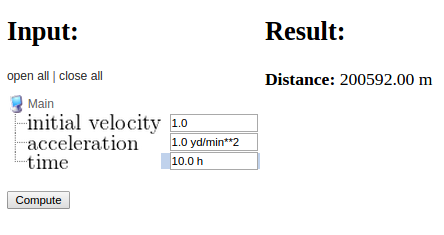
\includegraphics[width=0.5\linewidth]{fig-scaling/distance_GUI.png}}
  \caption{
  Web GUI where parameters can be specified with units. \label{scale:dimunit:fig:GUI}
  }
\end{figure}
%\clearpage % flush figures scale:dimunit:fig:GUI


With examples shown above, the reader should be able to make use of the
\texttt{PhysicalQuantity} object and the Parampool package in programs
and thereby work safely with units. For the coming text, where we discuss the
craft of scaling in detail, we shall just work in standard SI units
and avoid unit conversion so there will be no more use of
\texttt{PhysicalQuantity} and Parampool.


% !split
\chapter{Ordinary differential equation models}

This chapter introduces the basic techniques of scaling and the ways to
reason about scales. The first class of examples targets exponential
decay models, starting with the simple ordinary differential equation (ODE)
for exponential decay processes: $u^{\prime}=-au$, with constant $a>0$.
Then we progress to various generalizations of this ODE, including nonlinear
versions and systems of ODEs. The next class of examples concerns
second-order ODEs for oscillatory systems, where the simplest
ODE reads $mu^{\prime\prime} + ku=0$, with $m$ and $k$ as positive constants.
Various extensions with damping and force terms are discussed in detail.


\section{Exponential decay problems}
\label{sec:scale:decay}

\subsection{Fundamental ideas of scaling}


\index{scaling}
\index{non-dimensionalization}

Scaling is an extremely useful technique in mathematical modeling and
numerical simulation.  The purpose of the technique is three-fold:

\begin{enumerate}
\item Make independent and dependent variables dimensionless.

\item Make the size of independent and dependent variables about unity.

\item Reduce the number of independent physical parameters in the model.
\end{enumerate}

\noindent
\index{dimensionless variable}

The first two items mean that for any variable, denote it by
$q$, we introduce a corresponding dimensionless variable

\[ \bar q = \frac{q-q_0}{q_c},\]
where $q_0$ is a reference value of $q$ ($q_0=0$ is a common choice) and
$q_c$ is a characteristic size of $|q|$, often referred to as ``a scale''.
Since the numerator and denominator
have the same dimension, $\bar q$ becomes a dimensionless number.

If $q_c$ is the maximum value of $|q-q_0|$, we see that $0 < |\bar
q|\leq 1$. How to find $q_c$ is sometimes the big challenge of
scaling. Examples will illustrate various approaches to meet this
challenge.

The many coming examples on scaling differential equations contain
the following pedagogical ingredients to meet the desired learning outcomes.

\begin{itemize}
 \item Teach the technical steps of making a mathematical model, based
   on differential equations, dimensionless.

 \item Describe various techniques for reasoning about the scales, i.e.,
   finding the characteristic sizes of quantities.

 \item Teach how to identify and interpret dimensionless numbers arising
   from the scaling process.

 \item Provide a lot of different examples on making models dimensionless
   with physically correct scales.

 \item Show how symbolic software (SymPy) can be used
   to derive exact solutions of differential equations.

 \item Explain how to run a dimensionless model with software developed
   for the problem with dimensions.
\end{itemize}

\noindent
\subsection{The basic model problem}
\index{exponential decay}

Processes undergoing exponential reduction can be modeled by the ODE
problem

\begin{equation}
u'(t) = -au(t),\quad u(0)=I,
\label{scale:model}
\end{equation}
where $a,I>0$ are prescribed parameters, and $u(t)$ is the unknown function.
For the particular model with a constant $a$, we can easily derive the exact
solution, $u(t)=Ie^{-at}$,
which is helpful to have in mind during the scaling process.

\paragraph{Example: Population dynamics.}
The evolution of a population of humans, animals, cells, etc.,
under unlimited access to resources, can be
modeled by (\ref{scale:model}). Then $u$ is the number of
individuals in the population, strictly speaking an integer, but well
modeled by a real number in large populations.
The parameter $a$ is the increase in the number of individuals per
time and per individual.

\paragraph{Example: Decay of pressure with altitude.}
The simple model (\ref{scale:model}) also governs the pressure
in the atmosphere (under many assumptions, such air is an ideal gas in
equilibrium). In this case $u$ is the
pressure, measured in $\hbox{Nm}^{-2}$; $t$ is the height in meters;
and $a=M/(R^*T)$, where
$M$ is the molar mass of the Earth's air (0.029 kg/mol),
$R^*$ is the universal
gas constant ($8.314\,\frac{\hbox{Nm}}{\hbox{mol K}}$),
and $T$ is the temperature in Kelvin (K).
The temperature depends on the height so we have $a=a(t)$.


\subsection{The technical steps of the scaling procedure}
\label{sec:scale:steps}

\paragraph{Step 1: Identify independent and dependent variables.}
There is one independent variable, $t$, and one dependent variable,
$u$.

\index{dimensionless variable}
\index{characteristic time}

\paragraph{Step 2: Make independent and dependent variables dimensionless.}
We introduce a new dimensionless $t$, called $\bar t$, defined by
\begin{equation}
\bar t = \frac{t}{t_c},
\end{equation}
where $t_c$ is a \emph{characteristic value} of $t$. Similarly,
we introduce a dimensionless $u$, named $\bar u$, according to
\begin{equation}
\bar u = \frac{u}{u_c},
\end{equation}
where $u_c$ is a constant \emph{characteristic size} of $u$. When $u$ has a specific
interpretation, say when (\ref{scale:model}) models pressure
in an atmospheric layer, $u_c$ would be referred to as characteristic pressure.
For a decaying population, $u_c$ may be a characteristic number of
members in the population, e.g., the initial population $I$.

\paragraph{Step 3: Derive the model involving only dimensionless variables.}
The next task is to insert the new dimensionless variables in the
governing mathematical model. That is, we replace $t$ by $t_c\bar t$
and $u$ by $u_c\bar u$ in (\ref{scale:model}). The derivative
with respect to $\bar t$ is derived through the chain rule as

\[ \frac{du}{dt} = \frac{d (u_c\bar u)}{d\bar t}\frac{d\bar t}{dt}
= u_c\frac{d\bar u}{d\bar t}\frac{1}{t_c} =
\frac{u_c}{t_c}\frac{d\bar u}{d\bar t}\tp
\]
The model (\ref{scale:model}) now becomes

\begin{equation}
\frac{u_c}{t_c}\frac{d\bar u}{d\bar t} = -au_c\bar u,\quad u_c\bar u(0)=I\tp
\label{scale:model:scaled0}
\end{equation}

\paragraph{Step 4: Make each term dimensionless.}
Equation (\ref{scale:model:scaled0}) still has terms with
dimensions. To make each term dimensionless, we usually divide by
the coefficient in front of the term with the highest time derivative
(but dividing by any coefficient in any term will do). The result is

\begin{equation}
\frac{d\bar u}{d\bar t} = -at_c\bar u,\quad \bar u(0)=u_c^{-1}I
\tp
\label{scale:model:dimless0}
\end{equation}

\paragraph{Step 5: Estimate the scales.}
A characteristic quantity like $t_c$ reflects the time scale in the
problem. Estimating such a time scale is certainly
the most challenging part of the scaling procedure. There are different
ways to reason. The first approach
is to aim at a size of $\bar u$ and its derivatives
that is of order unity. If $u_c$ is chosen such that $|\bar u|$ is
of size unity, we see from (\ref{scale:model:dimless0}) that
$d\bar u/d\bar t$ is of the size of $\bar u$ (i.e., unity)
if we choose $t_c = 1/a$.

\index{e-folding time}

Alternatively, we may look at a special case of the model where we have
analytical insight that can guide the choice of scales.
In the present problem we are lucky to know the
exact solution for any value of the input data as long as $a$
is a constant. For exponential
decay,
$u(t)\sim e^{-at}$, it is common to define a characteristic time
scale $t_c$ as the time it takes to reduce the initial value of
$u$ by a factor of $1/e$ (also called the \emph{e-folding time}):

\[ e^{-at_c} = \frac{1}{e}e^{-a\cdot 0}\quad\Rightarrow\quad e^{-at_c}=e^{-1},
\]
from which it follows that $t_c = 1/a$.
Note that using an exact solution of the problem to determine
scales is not a requirement, just a useful help in the few cases where
we actually have access to an exact solution.

In this example, two different, yet common ways of reasoning, lead to the
same value of $t_c$. However, instead of using the e-folding time we
could use the half-time of the exponential decay as characteristic
time, which is also a very common measure of the time scale in such
processes. The half time is defined as the time it takes to halve $u$:

\[ e^{-at_c} = \frac{1}{2}e^{-a\cdot 0}
\quad\Rightarrow\quad t_c = a^{-1}\ln 2\tp\]
There is a factor $\ln 2 =0.69$ difference from the other $t_c$ value.
As long as the factor is not an order of magnitude or more different,
we do not pay attention factors like $\ln 2$ and skip them, simply to make
formulas look nicer. Using
$t_c = a^{-1}\ln 2$ as time scale
leads to a scaled differential equation $u'=-(\ln 2) u$,
which is fine, but an unusual form. People tend to prefer the simpler
ODE $u'=-u$,
which arises from $t_c=1/a$, and we shall therefore use this
time scale.

Regarding $u_c$, we may look at the initial condition and realize that
the choice $u_c=I$ makes $\bar u(0)=1$. For $t>0$, the differential
equation expresses explicitly that $u$ decreases, so $u_c=I$ gives
$\bar u\in (0, 1]$. Scaling a variable $q$ such that $|\bar q|\in
[0,1]$ is always the ultimate goal, and this goal is in fact obtained
here! Next best result is to ensure that the magnitude of $|q|$ is not
``big'' or ``small'', in the sense that the size is neither as large as
10 or 100, nor as small as
0.1 or 0.01.  (In the
present problem, where we are lucky to have an exact solution
$u(t)=Ie^{-at}$, we may look at this to explicitly see that $u\in
(0,I]$ such that $u_c=I$ gives $\bar u\in (0,1]$).

With $t_c=1/a$ and $u_c=I$, we have the final dimensionless model

\begin{equation}
\frac{d\bar u}{d\bar t} = -\bar u,\quad \bar u(0)=1
\tp
\label{scale:model:dimless}
\end{equation}
This is a remarkable result in the sense that \emph{all physical parameters}
($a$ and $I$)
are removed from the model! Or more precisely, there are no physical input
parameters to assign
before using the model. In particular, numerical investigations of the original
model (\ref{scale:model}) would need experiments with different
$a$ and $I$ values, while numerical investigations of
(\ref{scale:model:dimless}) can be limited to \emph{a single run}! As soon
as we have computed the curve $\bar u(\bar t)$, we can find the
solution $u(t)$ of (\ref{scale:model}) by

\begin{equation}
u(t) = u_c\bar u(t/t_c) = I\bar u(at)
\tp
\label{scale:u:dim}
\end{equation}
This particular transformation actually means stretching the $\bar t$ and
$\bar u$ axes in a plot of $\bar u(\bar t)$ by the factors $a$ and $I$,
respectively.

It is very common to drop the bars when the scaled problem has been
derived and work further with (\ref{scale:model:dimless}) simply
written as

\[
\frac{du}{dt} = -u,\quad u(0)=1
\tp
\]
Nevertheless, in this booklet we have decided to stick to bars for all
dimensionless quantities.


\subsection{Making software for utilizing the scaled model}
\label{sec:scale:prog}

Software for solving (\ref{scale:model}) could take advantage of
the fact that only one simulation of (\ref{scale:model:dimless})
is necessary. As soon as we have $\bar u(\bar t)$ accessible, a simple
scaling (\ref{scale:u:dim}) computes the real $u(t)$ for any
given input data $a$ and $I$. Although the numerical computation of
$u(t)$ from (\ref{scale:model}) is very fast in this simple model
problem, using (\ref{scale:u:dim}) is very much faster. In
general, a simple rescaling of a scaled solution is extremely more
computationally efficient than solving a differential equation
problem.

We can compute with the dimensionless model (\ref{scale:model:dimless})
in two ways, either make a solver for (\ref{scale:model:dimless}),
or reuse a solver for (\ref{scale:model}) with
$I=1$ and $a=1$.
We will choose the latter approach since it has the advantage of giving us
software that works both with a dimensionless model and a model
with dimensions (and all the original physical parameters).

\paragraph{Software for the original unscaled problem.}
Assume that we have some module \texttt{decay.py} that offers the following functions:

\begin{itemize}
  \item \texttt{solver(I, a, T, dt, theta=0.5)} for returning the solution arrays
    \texttt{u} and \texttt{t}, over a time interval $[0,T]$,
    for (\ref{scale:model}) solved by the so-called
    $\theta$ rule. This rule includes the Forward Euler scheme ($\theta=0$),
    the Backward Euler scheme ($\theta=1$), or the Crank-Nicolson
    (centered midpoint) scheme ($\theta=\half$).

  \item \Verb!read_command_line_argparse()! for reading parameters in the problem
    from the command line and returning them: \texttt{I}, \texttt{a}, \texttt{T}, \texttt{theta} ($\theta$),
    and a list of $\Delta t$ values for time steps. (We shall only make
    use of the first $\Delta t$ value.)
\end{itemize}

\noindent
The basic statements for solving (\ref{scale:model}) are
then

\begin{lstlisting}[language=Python,style=graycolor]
from decay import solver, read_command_line_argparse
I, a, T, theta, dt_values = read_command_line_argparse()
u, t = solver(I, a, T, dt_values[0], theta)

from matplotlib.pyplot import plot, show
plot(t, u)
show()
\end{lstlisting}
The module \href{{http://tinyurl.com/o8pb3yy/decay.py}}{\nolinkurl{decay.py}} is developed
and explained in
Section~\ref{softeng1:basic:module} in \cite{Langtangen_decay}.

To solve the dimensionless problem, just fix $I=1$ and $a=1$,
and choose $\bar T$ and $\Delta\bar t$:

\begin{lstlisting}[language=Python,style=graycolor]
_, _, T, theta, dt_values = read_command_line_argparse()
u, t = solver(I=1, a=1, T=T, dt=dt_values[0], theta=theta)
\end{lstlisting}
The first two variables returned from \Verb!read_command_line_argparse!
are \texttt{I} and \texttt{a}, which are ignored here. To indicate that these
variables are not to be used, we use a
``dummy name'', often taken to be the underscore symbol in
Python. The user can set \texttt{--I} and \texttt{--a} on the command line, since
the \texttt{decay} module allows this, but we hope the code above has a form
that reminds the user that these options are not to be used.
Also note that \texttt{T} and \Verb!dt_values[0]! set on the command line are
the desired parameters for solving the \emph{scaled} problem.


\paragraph{Software for the scaled problem.}
Turning now to the scaled problem, the solver function (originally
designed for the unscaled problem) will be reused, but it will only
be run if it is strictly necessary. That is, when the user requests
a solution, our code should first check whether that solution can be provided
by simply scaling a solution already computed and available in a file.
If not, we will compute an appropriate scaled solution, find the
requested unscaled solution for the user, and also save the new scaled
solution to file for possible later use.

% A key observation, as mentioned, is that we need to solve the problem
% (\ref{scale:model:dimless}) only once. All solutions
% corresponding to different $I$ and $a$ values in the original physical
% problem can be recovered by scaling this single solution with formula
% (\ref{scale:u:dim}).  We may therefore want to make software that
% takes advantage of this fact. When requesting a solution, we see if it
% has already been computed and stored in a file, and if so, the data
% can be retrieved from file, otherwise we have to compute a new
% solution and store it in a file.

A very plain solution to the problem is found in the file
\href{{http://tinyurl.com/o8pb3yy/decay_scaled_v1.py}}{\nolinkurl{decay_scaled_v1.py}}.
The \texttt{np.savetxt} function saves a two-dimensional array (``table'') to
a text file, and the \texttt{np.loadtxt} function can load the data back
into the program. A better solution to this problem is obtained
by using the \texttt{joblib} package as described next.

\index{memoize function}
\index{joblib@{\rm\texttt{joblib}}}

\paragraph{Implementation with joblib.}
The Python package \texttt{joblib} has functionality that is very convenient
for implementing the \Verb!solver_scaled! function. The first time a
function is called with a set of arguments, the statements in the
function are executed and the return value is saved to file. If the
function is called again with the same set of arguments, the
statements in the function are not executed, but the return value is
read from file (of course, many files may be stored, one for each
combination of parameter values).  In computer science, one would say
that \texttt{joblib} in this way provides \emph{memorization} functionality for
Python functions.  This functionality is particularly aimed at
large-scale computations with arrays that one would hesitate to
recompute. We illustrate the technique here in a very simple
mathematical context.

First we make a \Verb!solver_scaled! function for the scaled
model that just calls up a \Verb!solver_unscaled! (with $I=a=1$) for the problem with
dimensions:

\begin{lstlisting}[language=Python,style=graycolor]
from decay import solver as solver_unscaled
import numpy as np
import matplotlib.pyplot as plt

def solver_scaled(T, dt, theta):
    """
    Solve u'=-u, u(0)=1 for (0,T] with step dt and theta method.
    """
    print 'Computing the numerical solution'
    return solver_unscaled(I=1, a=1, T=T, dt=dt, theta=theta)
\end{lstlisting}
Then we create some ``computer memory on disk'', i.e., some disk space to
store the result of a call to the \Verb!solver_scaled! function. Thereafter,
we redefine the name \Verb!solver_scaled! to a new function, created
by \texttt{joblib}, which calls our original \Verb!solver_scaled! function
if necessary and otherwise loads data from file:

\begin{lstlisting}[language=Python,style=graycolor]
import joblib
disk_memory = joblib.Memory(cachedir='temp')
solver_scaled = disk_memory.cache(solver_scaled)
\end{lstlisting}
The solutions are actually stored in files in the cache directory \texttt{temp}.

A typical use case is to read values from the command line,
solve the scaled problem (if necessary), unscale the solution, and visualize
the solution with dimension:

\begin{lstlisting}[language=Python,style=graycolor]
def unscale(u_scaled, t_scaled, I, a):
    return I*u_scaled, a*t_scaled

from decay import read_command_line_argparse

def main():
    # Read unscaled parameters, solve and plot
    I, a, T, theta, dt_values = read_command_line_argparse()
    dt = dt_values[0]  # use only the first dt value
    T_bar = a*T
    dt_bar = a*dt
    u_scaled, t_scaled = solver_scaled(T_bar, dt_bar, theta)
    u, t = unscale(u_scaled, t_scaled, I, a)

    plt.figure()
    plt.plot(t_scaled, u_scaled)
    plt.xlabel('scaled time'); plt.ylabel('scaled velocity')
    plt.title('Universial solution of scaled problem')
    plt.savefig('tmp1.png');  plt.savefig('tmp1.pdf')

    plt.figure()
    plt.plot(t, u)
    plt.xlabel('t'); plt.ylabel('u')
    plt.title('I=%g, a=%g, theta=%g' % (I, a, theta))
    plt.savefig('tmp2.png'); plt.savefig('tmp2.pdf')
    plt.show()
\end{lstlisting}
The complete code resides in the file
\href{{http://tinyurl.com/o8pb3yy/decay_scaled.py}}{\nolinkurl{decay_scaled.py}}.
Note from the code above that \Verb!read_command_line_argparse! is supposed
to read parameters with dimensions (but technically, we solve the
scaled problem, if strictly necessary, and unscale the solution).
Let us run

\begin{Verbatim}[frame=lines,label=\fbox{{\tiny Terminal}},framesep=2.5mm,framerule=0.7pt,fontsize=\fontsize{9pt}{9pt}]
Terminal> python decay_scaled.py --I 8 --a 0.1 --dt 0.01 --T 50
\end{Verbatim}
A plot of the scaled and unscaled solution appears in Figure~\ref{sec:decay:fig:simplest}.


\begin{figure}[!ht]  % sec:decay:fig:simplest
  \centerline{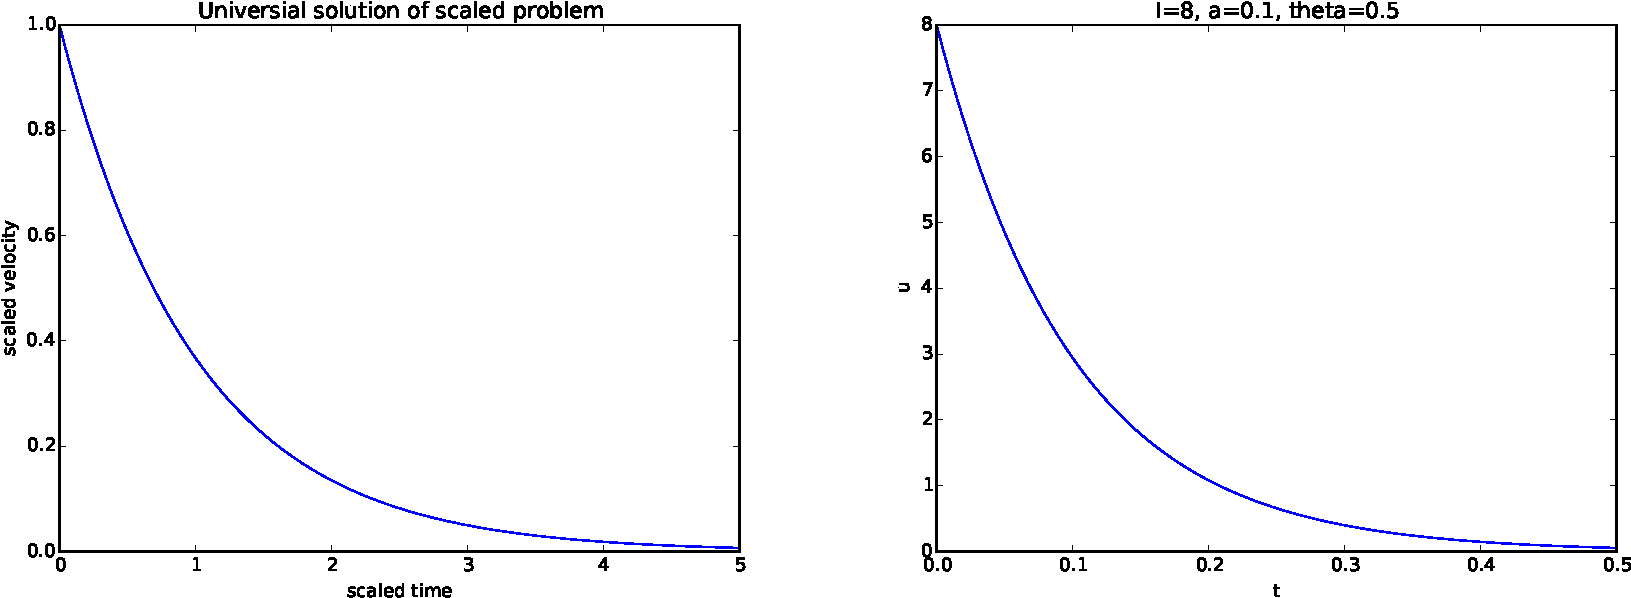
\includegraphics[width=1.0\linewidth]{fig-scaling/decay.pdf}}
  \caption{
  Scaled (left) and unscaled (right) exponential decay. \label{sec:decay:fig:simplest}
  }
\end{figure}
%\clearpage % flush figures sec:decay:fig:simplest



Note that we write a message \texttt{Computing the numerical solution} inside
the \Verb!solver_scaled! function. We can then easily detect when
the solution is actually computed from scratch
and when it is simply read from file (followed by the unscaling procedure).
Here is a demo:

\begin{Verbatim}[frame=lines,label=\fbox{{\tiny Terminal}},framesep=2.5mm,framerule=0.7pt,fontsize=\fontsize{9pt}{9pt}]
Terminal> # Very first run
Terminal> python decay_scaled.py --T 7 --a 1 --I 0.5 --dt 0.2
[Memory] Calling __main__--home-hpl...
solver_scaled-alias(7.0, 0.2, 0.5)
Computing the numerical solution

Terminal> # No change of T, dt, theta - can reuse solution in file
Terminal> python decay_scaled.py --T 7 --a 4 --I 2.5 --dt 0.2

Terminal> # Change of dt, must recompute
Terminal> python decay_scaled.py --T 7 --a 4 --I 2.0 --dt 0.5
[Memory] Calling __main__--home-hpl...
solver_scaled-alias(7.0, 0.5, 0.5)
Computing the numerical solution

Terminal> # Change of dt again, but dt=0.2 is already in a file
Terminal> python decay_scaled.py --T 7 --a 0.5 --I 1 --dt 0.2
\end{Verbatim}

We realize that \texttt{joblib} has access to all previous runs and does not
recompute unless it is strictly required. Our previous implementation
without \texttt{joblib} (in \Verb!decay_scaled_v1.py!)
used only one file (for one numerical case)
and will therefore perform many more calls to
\Verb!solver_unscaled!.



\begin{notice_mdfboxadmon}[On the implementation of a simple memoize function]
A memoized function recalls
previous results when the same set
of arguments is encountered. That is, the function caches its results.
A simple implementation stores the arguments in a function call and
the returned results in a
dictionary, and if the arguments are seen again, one looks up
in the dictionary and returns previously computed results:

\begin{lstlisting}[language=Python,style=graycolor]
class Memoize:
    def __init__(self, f):
        self.f = f
        self.memo = {}  # map arguments to results

def __call__(self, *args):
        if not args in self.memo:
            self.memo[args] = self.f(*args)
        return self.memo[args]

# Wrap my_compute_function(arg1, arg2, ...)
my_compute_function = Memoize(my_compute_function)
\end{lstlisting}
The memoize functionality in \texttt{joblib.Memory} is more sophisticated and
can work very efficiently with large array data structures as arguments.
Note that the simple version above can only be used when all arguments to
the function \texttt{f} are immutable (since the key in a dictionary has to be
immutable).
\end{notice_mdfboxadmon}



\subsection{Scaling a generalized problem}
\label{sec:scale:body}

Now we consider an extension of the exponential decay ODE to the
form

\begin{equation}
u'(t) = -au(t) + b,\quad u(0)=I
\label{scale:model:g}
\tp
\end{equation}
One particular model, with constant $a$ and $b$,
is a spherical small-sized organism falling in air,

\begin{equation}
u' = - \frac{3\pi d\mu}{\varrho_b V} u + g\left(\frac{\varrho}{\varrho_b} -1\right),
\label{scale:model:g:spec}
\end{equation}
where $d$, $\mu$, $\varrho_b$, $\varrho$, $V$, and $g$ are physical
parameters. The function $u(t)$ represents the vertical velocity,
being positive upwards.
We shall use this model in the following.

\paragraph{Exact solution.}
It can be handy to have the exact solution for reference, in case
of constant $a$ and $b$:

\[ \uex(t) = \frac{e^{-at}}{a}\left( b(e^{at}-1) + aI\right)
\tp
\]


\begin{notice_mdfboxadmon}[Solving differential equations in SymPy]
It can be very useful to use a symbolic computation tool such as SymPy
to aid us in solving differential equations.
Let us therefore demonstrate how SymPy can be used to find this solution.
First we define the parameters in the problem as symbols
and $u(t)$ as a function:

\begin{lstlisting}[language=Python,style=graycolor]
>>> from sympy import *
>>> t, a, b, I = symbols('t a b I', real=True, positive=True)
>>> u = symbols('u', cls=Function)
\end{lstlisting}
The next task is to define the differential equation, either as
a symbolic expression that is to equal zero, or as
an equation \texttt{Eq(lhs, rhs)} with \texttt{lhs} and \texttt{rhs} as expressions for
the left- and right-hand side):

\begin{lstlisting}[language=Python,style=graycolor]
>>> # Define differential equation
>>> eq = diff(u(t), t) + a*u(t) - b
>>> # or
>>> eq = Eq(diff(u(t), t), -a*u(t) + b)
\end{lstlisting}
The differential equation can be solved by the \texttt{dsolve} function, yielding
an equation of the form \texttt{u(t) == expression}. We want to grab the
expression on the right-hand side as our solution:

\begin{lstlisting}[language=Python,style=graycolor]
>>> sol = dsolve(eq, u(t))
>>> print sol
u(t) == (b + exp(a*(C1 - t)))/a
>>> u = sol.rhs                    # grab solution
>>> print u
(b + exp(a*(C1 - t)))/a
\end{lstlisting}
The solution contains the unknown integration constant \texttt{C1}, which must
be determined by the initial condition. We form the equation arising
from the initial condition $u(0)=I$:

\begin{lstlisting}[language=Python,style=graycolor]
>>> C1 = symbols('C1')
>>> eq = Eq(u.subs(t, 0), I)   # substitute t by 0 in u
>>> sol = solve(eq, C1)
>>> print sol
[log(I*a - b)/a]
\end{lstlisting}
The one solution that was found (stored in a list!)
must then be substituted back in the
expression \texttt{u} to yield the final solution:

\begin{lstlisting}[language=Python,style=graycolor]
>>> u = u.subs(C1, sol[0])
>>> print u
(b + exp(a*(-t + log(I*a - b)/a)))/a
\end{lstlisting}
As in mathematics with pen and paper, we strive to simplify
expressions also in symbolic computing software.
This frequently requires some trial and error
process with SymPy's simplification functions. A very standard
first try is to expand everything and run simplification algorithms:

\begin{lstlisting}[language=Python,style=graycolor]
>>> u = simplify(expand(u))
>>> print u
(I*a + b*exp(a*t) - b)*exp(-a*t)/a
\end{lstlisting}
Doing \texttt{latex(u)} automatically converts the expression to {\LaTeX} syntax
for inclusion in reports.
\end{notice_mdfboxadmon}



The reader may wonder why we bother with scaling of differential
equations if SymPy can solved the problem in a nice, closed
formula. This is true in the present introductory problem, but in a
more general problem setting, we have some differential equation where
SymPy perhaps can help with finding an exact solution only in a
special case. We can use this special-case solution to control our
reasoning about scales in the more general setting.

\paragraph{Theory.}
The challenges in our scaling is to find the right $u_c$ and $t_c$
scales. From (\ref{scale:model:g}) we see that if $u'\rightarrow 0$
as $t\rightarrow\infty$, $u$ approaches the constant value $b/a$. It can be
convenient to let the scaled $\bar u\rightarrow 1$ as
we approach the $d\bar u/d\bar t = 0$ state. This idea points to choosing

\begin{equation}
u_c = \frac{b}{a} = g\left(\frac{\varrho}{\varrho_b} -1\right)\left(\frac{3\pi d\mu}{\varrho_b V}\right)^{-1}
\tp
\end{equation}


\begin{notice_mdfboxadmon}[On the sign of the scaled velocity]
A little note on the sign of $u_c$ is necessary here.
With $\varrho_b < \varrho$, the buoyancy force upwards wins over the
gravity force downwards, and the body will move upwards. In this case,
the terminal velocity $u_c > 0$. When $\varrho_b > \varrho$, we get
a motion downwards, and $u_c < 0$. The corresponding $u$ is then also
negative, but the scaled velocity $u/u_c$, becomes positive.
\end{notice_mdfboxadmon}



\index{dimensionless number}

Inserting $u = u_c\bar u = b\bar u/a$ and $t=t_c\bar t$ in
(\ref{scale:model:g}) leads to

\[
\frac{d\bar u}{d\bar t} = -t_c a\bar u + \frac{t_c}{u_c}b,
\quad \bar u(0) = I\frac{a}{b}
\tp
\]
We want the scales such that $d\bar u/d\bar t$ and $\bar u$ are
about unity.
To balance the size of $\bar u$ and $d\bar u/d\bar t$ we must
therefore choose
$t_c = 1/a$, resulting in the scaled ODE problem

\begin{equation}
\frac{d\bar u}{d\bar t} = -\bar u + 1,\quad \bar u(0)=\beta,
\label{scale:model:g:dimless}
\end{equation}
where $\beta$ is a dimensionless number,
\begin{equation}
\beta = \frac{I}{u_c} = I\frac{a}{b},
\end{equation}
reflecting the ratio of the initial velocity and the
terminal ($t\rightarrow \infty$) velocity $b/a$.
Scaled equations normally end up with one or more dimensionless parameters,
such as $\beta$ here, containing ratios of physical effects in
the model. Many more examples on dimensionless parameters will appear
in later sections.

The analytical solution of the scaled model
(\ref{scale:model:g:dimless}) reads

\begin{equation}
\bar\uex(t) =
e^{-t}\left( e^{t}-1 + \beta\right) = 1 + (\beta -1)e^{-t}\tp
\label{scale:model:g:exact_scaled}
\end{equation}

The result (\ref{scale:model:g:dimless}) with the
solution (\ref{scale:model:g:exact_scaled}) is actually
astonishing if $a$ and $b$ are as in (\ref{scale:model:g:spec}):
the six parameters $d$, $\mu$, $\varrho_b$, $\varrho$, $V$, and $g$
are conjured to one:
\[ \beta = I\frac{3\pi d\mu}{\varrho_b V}
\frac{1}{g}\left(\frac{\varrho}{\varrho_b} -1\right)^{-1},
\]
which is an enormous simplification of the problem if our aim is to
investigate how $u$ varies with the physical input parameters in
the model.
In particular, if the motion starts from rest, $\beta=0$, and
there are no physical parameters in the scaled model!
We can then perform a single simulation and recover all physical
cases by the unscaling procedure. More precisely,
having computed $\bar u(\bar t)$ from (\ref{scale:model:g:dimless}),
we can use

\begin{equation}
u(t) = \frac{b}{a}\bar u(at),
\end{equation}
to scale back to the original
problem again.
We observe that (\ref{scale:model:g:dimless}) can utilize a solver
for (\ref{scale:model:g}) by setting $a=1$, $b=1$, and $I=\beta$.
Given some implementation of a solver for (\ref{scale:model:g}),
say \texttt{solver(I, a, b, T, dt, theta)},
the scaled model is run by \texttt{solver(beta, 1, 1, T, dt, theta)}.


\index{joblib@{\rm\texttt{joblib}}}

\paragraph{Software.}
We may develop a solver for the scaled problem that uses \texttt{joblib}
to cache solutions with the same $\beta$, $\Delta t$, and $T$.
For now we fix $\theta=0.5$.
The module \href{{http://tinyurl.com/o8pb3yy/decay_vc.py}}{\nolinkurl{decay_vc.py}}
(see Section~\ref{decay:general} in \cite{Langtangen_decay} for details)
has a function
\texttt{solver(I, a, b, T, dt, theta)} for solving $u'(t)=-a(t)u(t)+b(t)$ for
$t\in (0,T]$, $u(0)=I$, with time step \texttt{dt}.
We reuse this function and call it with $a=b=1$ and $I=\beta$ to solve
the scaled problem:

\begin{lstlisting}[language=Python,style=graycolor]
from decay_vc import solver as solver_unscaled

def solver_scaled(beta, T, dt, theta=0.5):
    """
    Solve u'=-u+1, u(0)=beta for (0,T]
    with step dt and theta method.
    """
    print 'Computing the numerical solution'
    return solver_unscaled(
        I=beta, a=lambda t: 1, b=lambda t: 1,
        T=T, dt=dt, theta=theta)

import joblib
disk_memory = joblib.Memory(cachedir='temp')
solver_scaled = disk_memory.cache(solver_scaled)
\end{lstlisting}
If we want to plot the physical solution, we need an \texttt{unscale} function,

\begin{lstlisting}[language=Python,style=graycolor]
def unscale(u_scaled, t_scaled, d, mu, rho, rho_b, V):
    a, b = ab(d, mu, rho, rho_b, V)
    return (b/a)*u_scaled, a*t_scaled

def ab(d, mu, rho, rho_b, V):
    g = 9.81
    a = 3*pi*d*mu/(rho_b*V)
    b = g*(rho/rho_b - 1)
    return a, b
\end{lstlisting}

Looking at droplets of water in air, we can fix some of the parameters
and let the size parameter $d$ be the one for experimentation.
The following function sets physical parameters, computes $\beta$,
runs the solver for the scaled problem (\texttt{joblib} detects
if it is necessary), and finally plots the scaled curve
$\bar u(\bar t)$ and the unscaled curve $u(t)$.

\begin{lstlisting}[language=Python,style=graycolor]
def main(dt=0.075, # Time step, scaled problem
         T=7.5,    # Final time, scaled problem
         d=0.001,  # Diameter (unscaled problem)
         I=0,      # Initial velocity (unscaled problem)
         ):
    # Set parameters, solve and plot
    rho = 0.00129E+3  # air
    rho_b = 1E+3      # density of water
    mu = 0.001        # viscosity of water
    # Asumme we have list or similar for d
    if not isinstance(d, (list,tuple,np.ndarray)):
        d = [d]

    legends1 = []
    legends2 = []
    plt.figure(1)
    plt.figure(2)
    betas = []     # beta values already computed (for plot)

    for d_ in d:
        V = 4*pi/3*(d_/2.)**3  # volume
        a, b = ab(d_, mu, rho, rho_b, V)
        beta = I*a/b
        # Restrict to 3 digits in beta
        beta = abs(round(beta, 3))

        print 'beta=%.3f' % beta
        u_scaled, t_scaled = solver_scaled(beta, T, dt)

        # Avoid plotting curves with the same beta value
        if not beta in betas:
            plt.figure(1)
            plt.plot(t_scaled, u_scaled)
            plt.hold('on')
            legends1.append('beta=%g' % beta)
        betas.append(beta)

        plt.figure(2)
        u, t = unscale(u_scaled, t_scaled, d_, mu, rho, rho_b, V)
        plt.plot(t, u)
        plt.hold('on')
        legends2.append('d=%g [mm]' % (d_*1000))
    plt.figure(1)
    plt.xlabel('scaled time'); plt.ylabel('scaled velocity')
    plt.legend(legends1, loc='lower right')
\end{lstlisting}
The most complicated part of the code is related to plotting, but
this part can be skipped when trying to understand how we work with
a scaled model to perform the computations.
The complete program is found in the file
\href{{http://tinyurl.com/o8pb3yy/falling_body.py}}{\nolinkurl{falling_body.py}}.

Since $I=0$ implies $\beta=0$, we can run different $d$ values without
any need to recompute $\bar u(\bar t)$ as long as we assume the particle
starts from rest.

From the scaling, we see that $u_c = b/a\sim d^{-2}$ and
also that $t_c=1/a \sim d^{-2}$, so plotting of $u(t)$ with dimensions
for various $d$ values will involve significant variations in the time
and velocity scales. Figure~\ref{sec:scale:body:fig}
has an example with $d=1,2,3$ mm, where we clearly see the different
time and velocity scales in the figure with unscaled variables.
Note that the scaled velocity is positive because of the sign of $u_c$
(see the box above).


\begin{figure}[!ht]  % sec:scale:body:fig
  \centerline{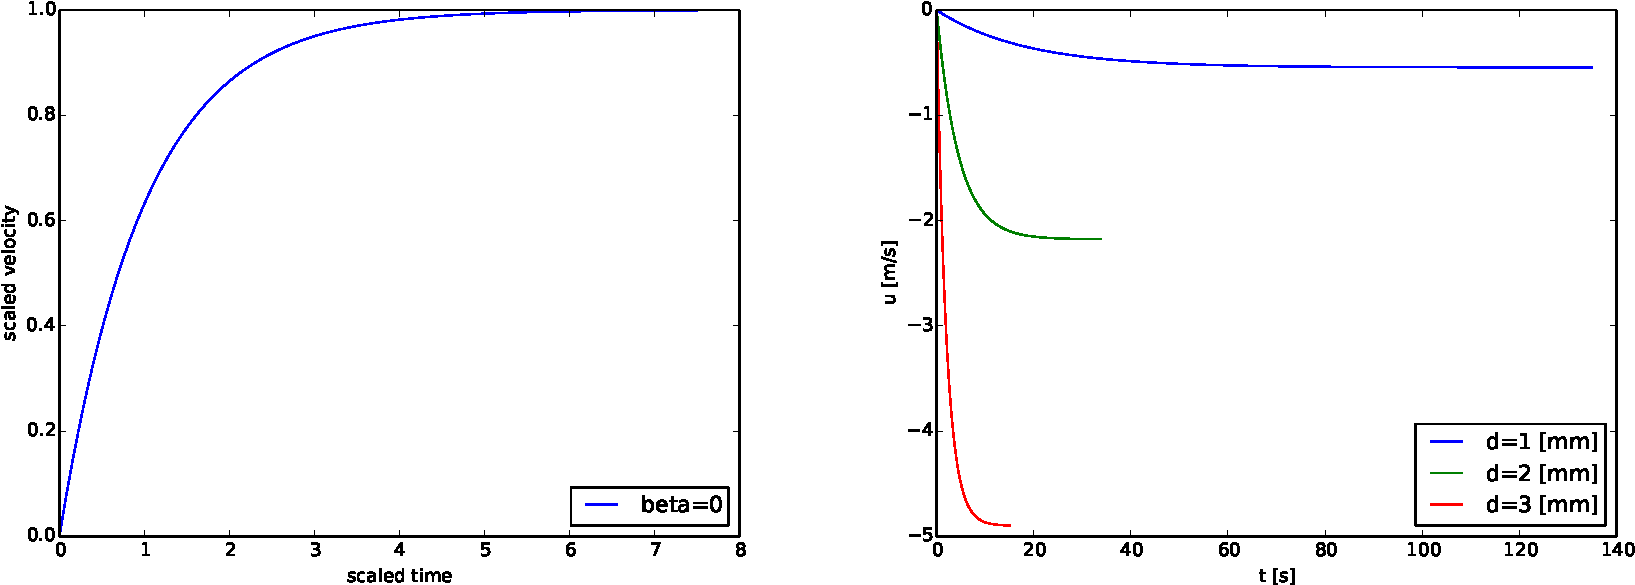
\includegraphics[width=1.0\linewidth]{fig-scaling/falling_body.pdf}}
  \caption{
  Velocity of falling body: scaled (left) and with dimensions (right). \label{sec:scale:body:fig}
  }
\end{figure}
%\clearpage % flush figures sec:scale:body:fig



\subsection{Variable coefficients}
\label{sec:scale:jump}

When a prescribed coefficient like $a(t)$ in $u'(t) = -a(t)u(t)$
varies with time one usually also
performs a scaling of this $a$,

\[ \bar a(\bar t) = \frac{a(t) - a_0}{a_c}, \]
where the goal is to have the scaled $\bar a$
of size unity: $|\bar a|\leq 1$.
This property is obtained by choosing $a_c$ as the maximum value
of $|a(t)-a_0|$ for $t\in [0,T]$, which is usually a quantity that
can be estimated since $a(t)$ is known as a function of $t$. The $a_0$
parameter can be chosen as 0 here. (It could be tempting to
choose $a_0=\min_t a(t)$ so that $0\leq \bar a\leq 1$, but then there
is at least one point where $\bar a = 0$ and
the differential equation collapses to $u'=0$.)

As an example, imagine a decaying cell culture where we at time $t_1$
change the environment (typically the nutrition)
such that the death rate increases by a factor 5.
Mathematically, $a(t) = d$ for
$t < t_1$ and $a(t)=5d$ for $t\geq t_1$. The model reads $u'=-a(t)u$, $u(0)=I$.

The $a(t)$ function is scaled by letting the characteristic size be
$a_c=d$ and $a_0=0$:

\[ \bar a (\bar t) = \left\lbrace\begin{array}{ll}
1, & \bar t < t_1/t_c\\ 
5, & \bar t \geq t_1/t_c
\end{array}\right.
\]

\index{dimensionless number}

The scaled equation becomes

\[ \frac{u_c}{t_c}\frac{d\bar u}{d\bar t} = a_c\bar a(\bar t) u_c\bar u,\quad
u_c\bar u(0) = I\tp\]
The natural choice of $u_c$ is $I$.
The characteristic time, previously taken as $t_c=1/a$, can now be
chosen as $t_c=t_1$ or $t_c=1/d$.
With $t_c=1/d$ we get

\begin{equation}
\bar u'(\bar t)=-\bar a\bar u,\quad \bar u(0)=1,\quad
\bar a = \left\lbrace\begin{array}{ll}
1, & \bar t < \gamma\\ 
5, & \bar t \geq \gamma
\end{array}\right.
\label{sec:scale:jump:eq1}
\end{equation}
where

\[ \gamma = t_1 d\]
is a dimensionless number in the problem. With $t_c=t_1$, we get

\[ \bar u'(\bar t)=-\gamma\bar a\bar u,\quad \bar u(0)=1,\quad
\bar a = \left\lbrace\begin{array}{ll}
1, & \bar t < 1\\ 
5, & \bar t \geq 1
\end{array}\right.\]
The dimensionless parameter $\gamma$ is now in the equation rather than in
the definition of $\bar a$. Both problems involve $\gamma$, which
is the ratio between the time when the environmental change happens
and the typical time for the decay ($1/d$).

A computation with the scaled model (\ref{sec:scale:jump:eq1})
and the original model with dimensions appears in
Figure~\ref{sec:scale:jump:fig}.


\begin{figure}[!ht]  % sec:scale:jump:fig
  \centerline{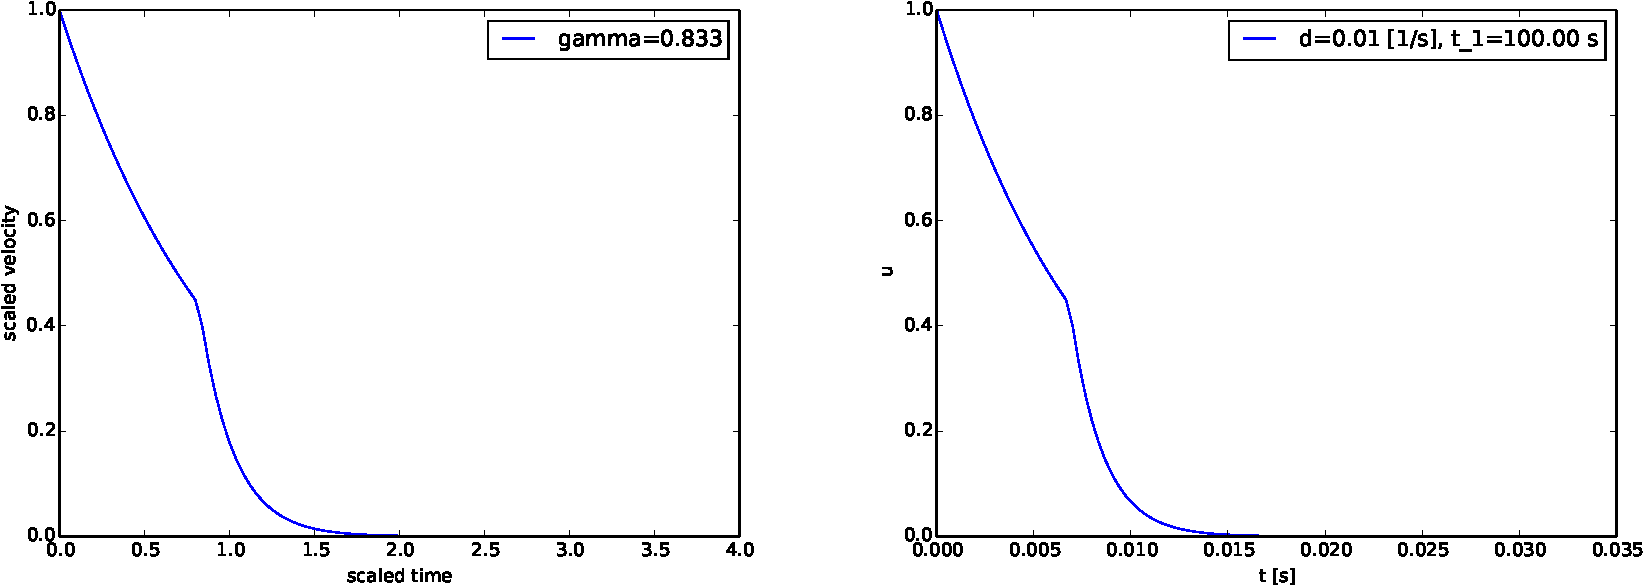
\includegraphics[width=1.0\linewidth]{fig-scaling/decay_jump.pdf}}
  \caption{
  Exponential decay with jump: scaled model (left) and unscaled model (right). \label{sec:scale:jump:fig}
  }
\end{figure}
%\clearpage % flush figures sec:scale:jump:fig



\subsection{Scaling a cooling problem with constant temperature in the surroundings}
\label{scale:cooling:const}

The heat exchange between a body at temperature $T(t)$ and the
surroundings at constant temperature $T_s$
can be modeled by Newton's law of cooling:

\begin{equation}
T'(t) = -k(T-T_s),\quad T(0)=T_0,
\label{scale:cooling:model}
\end{equation}
where $k$ is a prescribed heat transfer coefficient.

\paragraph{Exact solution.}
An analytical solution is always handy to have as a control of the
choice of scales. The solution of (\ref{scale:cooling:model})
is by standard methods for ODEs found to be
$T(t) = T_s + (T_0 - T_s)e^{-kt}$.

\paragraph{Scaling.}
Physically, we expect the temperature to start at $T_0$ and then to
move toward the temperature of the surroundings ($T_s$). We therefore
expect that $T$ lies between $T_0$ and $T_s$. This is mathematically
demonstrated by the analytical solution as well. A proper scaling is
therefore to scale and translate $T$ according to

\begin{equation}
\bar T = \frac{T-T_0}{T_s-T_0}
\label{scale:cooling:Tbar}
\tp
\end{equation}
Now, $0\leq \bar T\leq 1$.

Scaling time by $\bar t = t/t_c$ and inserting
$T= T_0 + (T_s-T_0)\bar T$ and $t=t_c\bar t$ in the
problem (\ref{scale:cooling:model}) gives

\[ \frac{d\bar T}{d\bar t} = - t_ck(\bar T - 1),\quad \bar T(0) = 0
\tp
\]
A natural choice, as argued in other exponential decay problems,
is to choose $t_ck=1$, which leaves us with the scaled problem

\begin{equation}
\frac{d\bar T}{d\bar t} = - (\bar T - 1),\quad \bar T(0)=0
\label{scale:cooling:Tbar:eq}
\tp
\end{equation}
No physical parameter enters this problem!
Our scaling implies that $\bar T$ starts at
0 and approaches 1 as $\bar t\rightarrow\infty$, also in the case
$T_s < T_0$. The physical temperature is always recovered as
\begin{equation}
T(t) = T_0 + (T_s-T_0)\bar T (k\bar t)
\label{scale:cooling:T}
\tp
\end{equation}

\paragraph{Software.}
An implementation for (\ref{scale:cooling:model}) works for
(\ref{scale:cooling:Tbar:eq}) by setting $k=1$, $T_s=1$, and $T_0=0$.

\paragraph{Alternative scaling.}
An alternative temperature scaling is to choose
\begin{equation}
\bar T = \frac{T-T_s}{T_0-T_s}
\label{scale:cooling:Tbar2}
\tp
\end{equation}
Now $\bar T=1$ initially and approaches zero as $t\rightarrow\infty$.
The resulting scaled ODE problem then becomes

\begin{equation}
\frac{d\bar T}{d\bar t} = - \bar T,\quad \bar T(0)=1,
\label{scale:cooling:Tbar:eq2}
\tp
\end{equation}
with solution $\bar T = e^{-\bar t}$.

\subsection{Scaling a cooling problem with time-dependent surroundings}
\label{scale:cooling:osc}

Let us apply the model (\ref{scale:cooling:model}) to the case when
the surrounding temperature varies in time. Say we have
an oscillating temperature environment according to

\begin{equation}
T_s(t) = T_m + a\sin(\omega t),
\label{scale:cooling:Tst}
\end{equation}
where $T_m$ is the mean temperature in the surroundings, $a$ is
the amplitude of the variations around $T_m$, and $2\pi/\omega$ is
the period of the temperature oscillations.

\paragraph{Exact solution.}
Also in this relatively simple problem
it is possible to solve the differential equation problem analytically.
Such a solution may be a good help to see what the scales are, and
especially to control other forms for reasoning about the scales.
Using the method of integrating factors for the
original differential equation, we have

\[ T(t) = T_0e^{-kt} + e^{-kt}k\int_0^t e^{k\tau}T_s(\tau)d\tau\tp\]
With $T_s(t)=T_m + a\sin (\omega t)$ we can use SymPy to help us with
integrations (note that we use \texttt{w} for $\omega$ in the computer code):

\begin{lstlisting}[language=Python,style=graycolor]
>>> from sympy import *
>>> t, k, T_m, a, w = symbols('t k T_m a w', real=True, positive=True)
>>> T_s = T_m + a*sin(w*t)
>>> I = exp(k*t)*T_s
>>> I = integrate(I, (t, 0, t))
>>> Q = k*exp(-k*t)*I
>>> Q = simplify(expand(Q))
>>> print Q
(-T_m*k**2 - T_m*w**2 + a*k*w +
(T_m*k**2 + T_m*w**2 + a*k**2*sin(t*w) -
a*k*w*cos(t*w))*exp(k*t))*exp(-k*t)/((k**2 + w**2))
\end{lstlisting}
Reordering the result, we get

\[ T(t) = T_0e^{-kt} + T_m(1- e^{-kt}) +  (k^2 + \omega^2)^{-1}(ak\omega e^{-kt}
+ ak\sin (\omega t) - akw\cos(\omega t))\tp\]

\index{dimensionless number}

\paragraph{Scaling.}
The scaling (\ref{scale:cooling:Tbar}) brings in a time-dependent
characteristic temperature scale $T_s-T_0$. Let us start with a
fixed scale, where we take the characteristic temperature variation to
be $T_m - T_0$:

\[ \bar T = \frac{T-T_0}{T_m-T_0}\tp\]
We realize by physical
reasoning that $T$ sets out at $T_0$, but with time, it will oscillate
around $T_m$. (This reasoning can be controlled by looking at the exact
solution we produced above.)
The typical average temperature span is therefore
$|T_m-T_0|$, unless $a$ is much larger than $|T_m-T_0|$ or $T_0$ is
very close to
$T_m$.

We get from the differential equation, with $t_c=1/k$ as in the former
case,

\[ k(T_m-T_0)\frac{d\bar T}{d\bar t} = -k((T_m-T_0)\bar T + T_0 - T_m - a
\sin(\omega t),\]
resulting in

\begin{equation}
\frac{d\bar T}{d\bar t} = -\bar T + 1 + \alpha\sin (\beta \bar t),\quad
\bar T(0)=0,
\label{scale:cooling:model:scaled}
\end{equation}
where we have two dimensionless numbers:

\[ \alpha = \frac{a}{T_m-T_0},\quad \beta = \frac{\omega}{k}\tp\]
The $\alpha$ quantity measures the ratio of temperatures: amplitude of
oscillations versus distance from initial temperature to the average
temperature for large times.  The $\beta$ number is the ratio of the
two time scales: the frequency of the oscillations in $T_s$ and the
inverse e-folding time of the heat transfer. For clear interpretation
of $\beta$ we may introduce the period $P=2\pi/\omega$ of the
oscillations in $T_s$ and the e-folding time $e=1/k$. Then $\beta =
2\pi e/P$ and measures the e-folding time versus the period.


\begin{notice_mdfboxadmon}[Remark]
The original problem features five physical parameters: $k$, $T_0$,
$T_m$, $a$, and $\omega$, but only two dimensionless numbers appear in the
scaled model (\ref{scale:cooling:model:scaled}).
In fact, this is an example where application of the Pi theorem
(see Section~\ref{scale:dimunit:Pi}) falls
short. Since, only time and temperature are involved as unit types, the
theorem predicts that the five parameters yields three dimensionless numbers,
not two. Scaling of the differential equations, on the other hand,
shows us that the two parameters
$T_m$ and $T_0$ affect the nature of the problem only through their difference.
\end{notice_mdfboxadmon}



\paragraph{Software.}
Implementations of the unscaled problem (\ref{scale:cooling:model})
can be reused for the scaled model by setting $k=1$, $T_0=0$, and
$T_s(t) = 1 + \alpha\sin (\beta \bar t)$ ($T_m=1$, $a=\alpha$, $\omega =\beta$).
The file \href{{http://tinyurl.com/o8pb3yy/osc_cooling.py}}{\nolinkurl{osc_cooling.py}} contains
solvers for the problem with dimensions and
for the scaled problem. The figure below
shows three cases of $\beta$ values: small, medium, and large.



% inline figure
\centerline{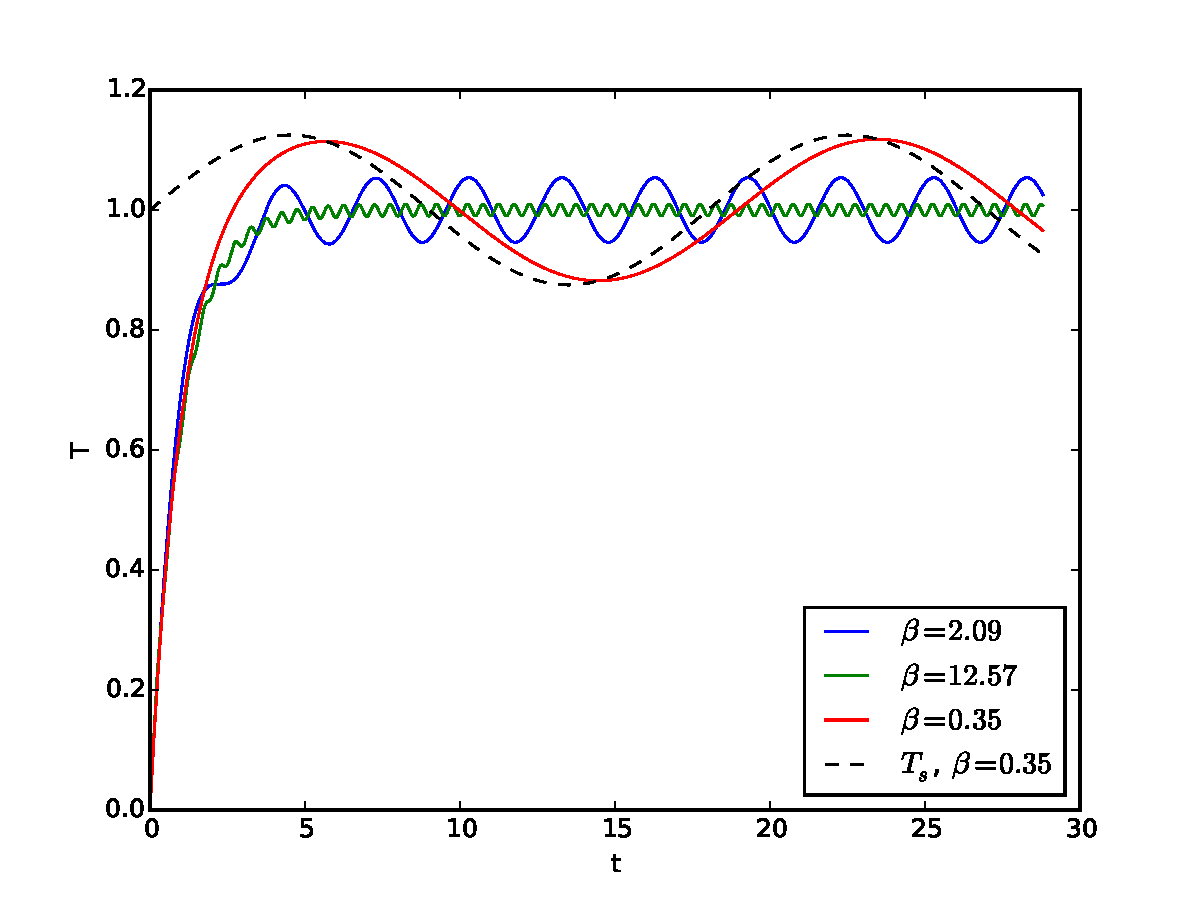
\includegraphics[width=0.8\linewidth]{fig-scaling/osc_cooling.pdf}}



For the small $\beta$ value, the oscillations in the surrounding
temperature are slow enough compared to $k$ for the heating and
cooling process to follow the surrounding temperature, with a small
time lag. For larger $\beta$, the heating and cooling require more
time, and the oscillations get smaller.

\paragraph{Discussion of the time scale.}
There are two time variations of importance in the present problem:
heat is transferred to the surroundings at a rate $k$, and the
surroundings have a temperature variation with a period that goes like
$1/\omega$. (We can, when we are so lucky that we have an analytical
solution at hand, inspect this solution to see that $k$ impacts the
problem through a decay factor $e^{-kt}$, and $\omega$ impacts the problem
through oscillations $\sin(\omega t)$.)  The $k$ parameter related to
temperature decay points to a time scale $t_c=1/k$, while the
temperature oscillations of the surroundings point to a time scale
$t_c=1/\omega$.  Which one should be chosen?

Bringing the temperature from $T_0$ to the level of the surroundings,
$T_m$, goes like $e^{-kt}$, so in this process $t_c=1/k$ is the
characteristic time. Thereafter, the body's temperature just responds
to the oscillations and the $\sin (\omega t)$ (and $\cos(\omega t)$)
term dominates. For these large times, $t_c=1/\omega$ is the
appropriate time scale. Choosing $t_c=1/\omega$ results in

\begin{equation}
\frac{d\bar T}{d\bar t} = -\beta^{-1}(\bar T - (1 + \alpha\sin (\bar t))),\quad
\bar T(0)=0\tp
\label{scale:cooling:model:scaled2}
\end{equation}


Let us illustrate another, less effective, scaling.
The temperature scale in
(\ref{scale:cooling:Tbar}) looks natural, so we apply this
choice of scale. The characteristic temperature $T_0-T_s$
now involves
a time-dependent term $T_s(t)$. The mathematical steps become a bit
more technically involved:

\[ T(t) = T_0 + (T_s(t)-T_0)\bar T,\]

\[ \frac{dT}{dt} = \frac{dT_s}{dt}\bar T +
(T_s-T_0)\frac{d\bar T}{d\bar t}\frac{d\bar t}{dt}
\tp
\]
With $\bar t = t/t_c = kt$ we get from the differential equation

\[
\frac{dT_s}{dt}\bar T +
(T_s-T_0)\frac{d\bar T}{d\bar t}k
= -k(\bar T - 1)(T_s - T_0),
\]
which after dividing by $k(T_s-T_0)$ results in

\[
\frac{d\bar T}{d\bar t} = -(\bar T - 1) -
\frac{dT_s}{dt}\frac{\bar T}{k(T_s-T_0},
\]
or

\[
\frac{d\bar T}{d\bar t} = -(\bar T - 1) -
\frac{a\omega\cos(\omega \bar t/k)}{k(T_m + a\sin(\omega \bar t/k) -T_0)}\bar T
\tp
\]
The last term is complicated and becomes more tractable if we factor
out dimensionless numbers. To this end, we scale $T_s$ by (e.g.) $T_m$,
which means to factor out $T_m$ in the denominator. We are then
left with

\begin{equation}
\frac{d\bar T}{d\bar t} = -(\bar T - 1) -
\alpha\beta \frac{\cos(\beta \bar t)}{1 + \alpha\sin(\beta\bar t) - \gamma}
\bar T,
\label{scale:cooling:Tbar:eq3}
\end{equation}
where $\alpha$, $\beta$, and $\gamma$ are dimensionless numbers
characterizing the relative importance of parameters in the problem:

\begin{equation}
\alpha=a/T_m,\quad \beta = \omega/k,\quad \gamma = T_0/T_m
\tp
\end{equation}
We notice that (\ref{scale:cooling:Tbar:eq3})
is not a special case of the original problem
(\ref{scale:cooling:model}). Furthermore, the original five
parameters $k$, $T_m$, $a$, $\omega$, and
$T_0$ are reduced to three dimensionless parameters.
We conclude that this scaling is inferior, because
using the temperature scale $T_0-T_m$ enables reuse of the software
for the unscaled problem and only two dimensionless parameters appear
in the scaled model.

Let us briefly mention another possible temperature scaling:
$\bar T = T/T_m$, motivated by the fact that as $t\rightarrow\infty$,
$T$ will oscillate around $T_m$, so this $\bar T$ will oscillate around
unity. We get the dimensionless ODE

\[ \frac{d\bar T}{d\bar t} = -(\bar T - (1 + \delta\sin(\beta\bar t))),\]
with a new dimensionless parameter $\delta = a/T_m$. However, the initial
condition becomes $\bar T(0)=T_0/T_m$, and the ratio $T_0/T_m$ is
a third dimensionless parameter, so this scaling is also inferior to the
one above with only two parameters.

\subsection{Scaling a nonlinear ODE}
\label{sec:scale:nonlinear}

\index{logistic equation}

Exponential growth models, $u'=au$, are not realistic in environments
with limited resources. However, by letting $a$ depend on $u$, the effect
of limited resources can well be captured by such a simple differential
equation model:

\begin{equation}
u' = a(u)u,\quad u(0)=I\tp
\label{sec:scale:nonlinear:model1}
\end{equation}
If the maximum value of $u$ is denoted by $M$, we have that $a(M)=0$.
A simple choice fulfilling this requirement is $a(u)=\varrho(1-u/M)$.
The parameter $\varrho$ can be interpreted as the initial exponential
growth rate if we assume that $I/M\ll 1$, since at $t=0$ the model then
approximates $u'=\varrho u$.

The choice $a(u)=\varrho(1-u/M)$ is known as the logistic model for
population growth:

\begin{equation}
u' = \varrho u(1-u/M),\quad u(0)=I\tp
\label{sec:scale:nonlinear:model2}
\end{equation}
A more complicated choice of $a$ may be $a(u)=\varrho(1-u/M)^p$ for
some exponent $p$ (this function also fulfills $a(M)=0$ and $a\approx\varrho$
for $t=0$).

\index{dimensionless number}

\paragraph{Scaling.}
Let us scale (\ref{sec:scale:nonlinear:model1}) with
$a(u)=\varrho (1-u/M)^p$.
The natural scale for $u$ is $M$ ($u_c=M$), since we know that
$0 < u\leq M$, and this makes the dimensionless $\bar u = u/M \in (0,1]$.
The function $a(u)$ is
typically varying between 0 and $\varrho$, so it can be scaled as

\[ \bar a(\bar u) = \frac{a(u)}{\varrho} = (1 - \frac{u}{M})^p =
(1 - \bar u)^p\tp\]
Time is scaled as $\bar t = t/t_c$ for some suitable characteristic time $t_c$.
Inserted in (\ref{sec:scale:nonlinear:model1}), we get

\[ \frac{u_c}{t_c}\frac{d\bar u}{d\bar t} = \varrho\bar a u_c\bar u,\quad u_c\bar u(0)=I,\]
resulting in

\[ \frac{d\bar u}{d\bar t} = t_c \varrho (1 - \bar u)^p \bar u,\quad
\bar u(0) =\frac{I}{M}\tp\]
A natural choice is $t_c =1/\varrho$ as in other exponential growth models
since it leads to the term on the right-hand side to be about unity,
just as the left-hand side. (If the scaling is correct, $\bar u$ and its
derivatives are of order unity, so the coefficients must also be of order
unity.) Introducing also the dimensionless parameter

\[ \alpha = \frac{I}{M},\]
measuring the fraction of the initial population compared to the maximum
one, we get the dimensionless model

\begin{equation}
\frac{d\bar u}{d\bar t} = (1 - \bar u)^p \bar u,\quad
\bar u(0) =\alpha\tp
\label{sec:scale:nonlinear:model1:scaled}
\end{equation}
Here, we have two dimensionless parameters: $\alpha$ and $p$. A classical
logistic model with $p=1$ has only one dimensionless variable.

\paragraph{Alternative scaling.}
We could try another scaling of $u$ where we also translate $\bar u$:

\[ \bar u = \frac{u-I}{M}\tp \]
This choice of $\bar u$ results in

\begin{equation}
\frac{d\bar u}{d\bar t} = (1 - \alpha - \bar u)^p \bar u,\quad
\bar u(0) =0\tp
\label{sec:scale:nonlinear:model1:scaled2}
\end{equation}
The essential difference between (\ref{sec:scale:nonlinear:model1:scaled})
and (\ref{sec:scale:nonlinear:model1:scaled2}) is that
$\bar u\in [\alpha, 1]$ in the former and $\bar u \in [0, 1-\alpha]$ in
the latter. Both models involve the dimensionless numbers $\alpha$ and $p$.
An advantage of (\ref{sec:scale:nonlinear:model1:scaled})
is that software for the unscaled model can easily be used for the
scaled model by choosing $I=\alpha$, $M=1$, and $\varrho=1$.

\subsection{SIR ODE system for spreading of diseases}

The field of epidemiology frequently applies ODE systems to describe
the spreading of diseases, such as smallpox, measles, plague, ordinary
flu, swine flu, and HIV. Different models include different effects,
which are reflected in dimensionless numbers. Most of the effects are
modeled as exponential decay or growth of the dependent variables.

The simplest model has three categories of people: susceptibles (S)
who can get the disease, infectious (I) who are infected and may
infect susceptibles, and recovered (R) who have recovered from the
disease and gained immunity. We introduce $S(t)$, $I(t)$, and $R(t)$
as the number of people in the categories S, I, and R, respectively.
The model, naturally known as the \href{{https://en.wikipedia.org/wiki/Epidemic_model}}{SIR model}\footnote{\texttt{https://en.wikipedia.org/wiki/Epidemic\_model}}, can be expressed as a
system of three ODEs:

\begin{align}
\frac{dS}{dt} &= - \beta SI,
\label{scale:SIR:S}\\ 
\frac{dI}{dt} &= \beta SI - \nu I,
\label{scale:SIR:I}\\ 
\frac{dR}{dt} &= \nu I,
\label{scale:SIR:R}
\end{align}
where $\beta$ and $\nu$ are empirical constants. The average time for recovering
from the disease can be shown to be $\nu^{-1}$, but $\beta$ is much harder
to estimate, so working with a scaled model where $\beta$ is ``scaled away''
is advantageous.

\paragraph{Scaling.}
It is natural to scale $S$, $I$, and $R$ by, e.g., $S(0)$:

\[ \bar S = \frac{S}{S(0)},\quad \bar I = \frac{I}{S(0)},\quad
\bar R = \frac{R}{S(0)}\tp
\]
Introducing $\bar t = t/t_c$, we arrive at the equations

\begin{align*}
\frac{d\bar S}{d\bar t} &= - t_c S(0) \beta\bar S\bar I,
\\ 
\frac{d\bar I}{d\bar t} &= t_c S(0) \beta \bar S\bar I - t_c \nu \bar I,
\\ 
\frac{d\bar R}{d\bar t} &= t_c \nu \bar I,
\end{align*}
with initial conditions $\bar S(0)=1$, $\bar I(0)=I_0/S(0)=\alpha$, and
$\bar R(0)=R(0)/S(0)$. Normally, $R(0)=0$.

Taking $t_c=1/\nu$, corresponding to a time unit equal to the time it takes
to recover from the disease, we end up with the scaled model

\begin{align}
\frac{d\bar S}{d\bar t} &= - R_0\bar S\bar I,
\label{scale:SIR:S2}\\ 
\frac{d\bar I}{d\bar t} &= R_0 \bar S\bar I - \bar I,
\label{scale:SIR:I2}\\ 
\frac{d\bar R}{d\bar t} &= \bar I,
\label{scale:SIR:R2}
\end{align}
with $\bar S(0)=1$, $\bar I(0)=\alpha$, $\bar R(0)=0$, and $R_0$ as
the dimensionless number

\begin{equation}
R_0 = \frac{S(0)\beta}{\nu}\tp
\end{equation}
We see from (\ref{scale:SIR:I2}) that to make the disease spreading,
$d\bar I/d\bar t >0$, and therefore $R_0 \bar S(0) - 1 > 0$ or $R_0 > 1$
since $\bar S(0)=1$.
Therefore, $R_0$ reflects the disease's ability to spread and is
consequently an important dimensionless quantity, known as the \href{{https://en.wikipedia.org/wiki/Basic_reproduction_number}}{basic
reproduction number}\footnote{\texttt{https://en.wikipedia.org/wiki/Basic\_reproduction\_number}}.
This number reflects the number of infected people caused by one infectious
individual during the time period of the disease.

Looking at (\ref{scale:SIR:I}), we see that to increase $I$ initially,
we must have $dI/dt >0$ at $t=0$, which implies
$\beta I(0)S(0) - \nu I(0) >0$, i.e., $R_0 > 1$.

\paragraph{Software.}
Any implementation of the SIR model with dimensions can be reused for
the scaled model by setting $\beta = R_0$, $\nu = 1$, $S(0)=1-\alpha$,
and $I(0)=\alpha$. Below is a plot with two cases: $R_0=2$ and $R_0=5$,
both with $\alpha=0.02$.



\vspace{3mm}




\vspace{3mm}





% inline figure
\centerline{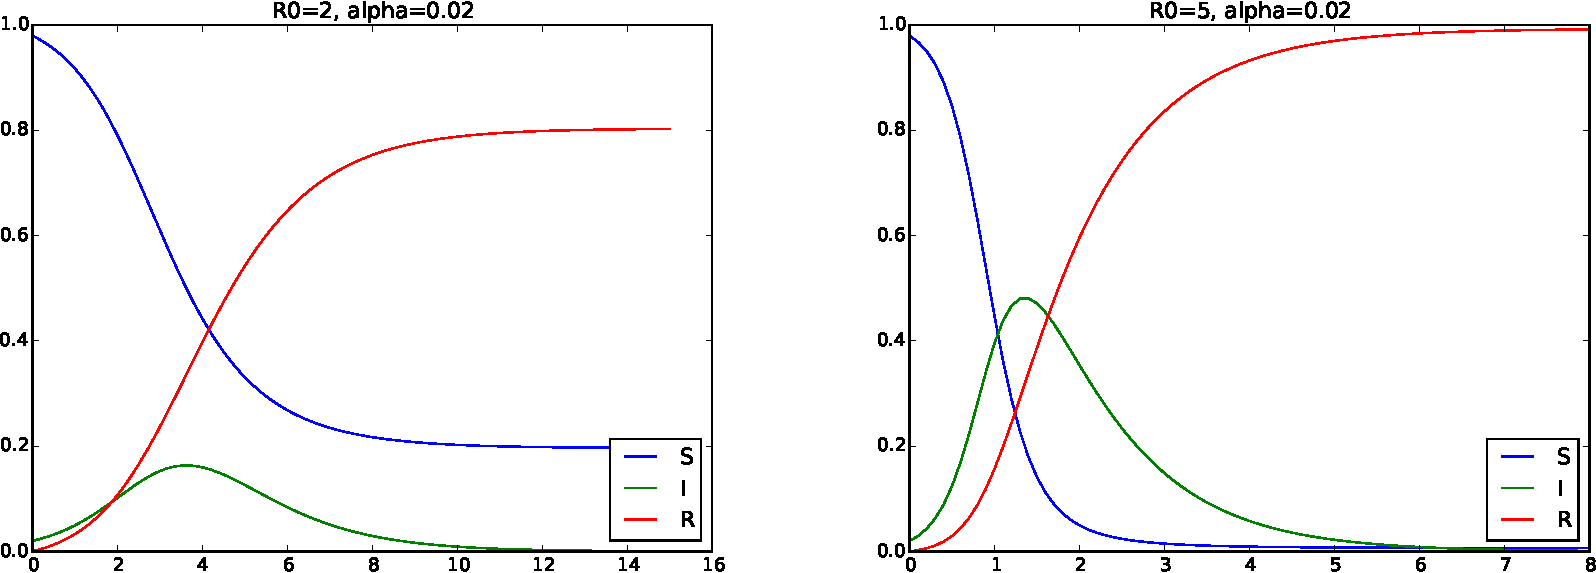
\includegraphics[width=1.0\linewidth]{fig-scaling/SIR1.pdf}}





\vspace{3mm}




\vspace{3mm}




\paragraph{Alternative scaling.}
Adding (\ref{scale:SIR:S})-(\ref{scale:SIR:R}) shows that

\[ \frac{dS}{dt}+\frac{dI}{dt}+\frac{dR}{dt}=0\quad\Rightarrow\quad
S+I+R=\hbox{const}=N,\]
where $N$ is the size of the population.
We can therefore scale $S$, $I$, and $R$ by the total
population $N=S(0)+I(0)+R(0)$:

\[ \bar S = \frac{S}{N},\quad \bar I = \frac{I}{N},\quad
\bar R = \frac{R}{N}\tp
\]
With the same time scale, one gets the system (\ref{scale:SIR:S2})-(\ref{scale:SIR:R2}), but with $R_0$ replaced by the dimensionless number:

\begin{equation}
\tilde R_0 = \frac{N\beta}{\nu}\tp
\end{equation}
The initial conditions become $\bar S(0)=1-\alpha$, $\bar I(0)=\alpha$,
and $\bar R(0)=0$.

For the disease to spread at $t=0$, we must have $\tilde R_0 \bar S(0) > 1$,
but $\tilde R_0 \bar S(0) = N\beta/\nu \cdot S(0)/N = R_0$, so the
criterion is still $R_0 > 1$. Since $R_0$ is a more famous number than
$\tilde R_0$, we can write the ODEs with $R_0/S(0) = R_0/(1-\alpha)$
instead of $\tilde R_0$.

Choosing $t_c$ to make the $SI$ terms balance the time derivatives,
$t_c = (N\beta)^{-1}$, moves $\tilde R_0$ (or $R_0$ if we scale
$S$, $I$, and $R$ by $S(0)$) to the $I$ terms:

\begin{align*}
\frac{d\bar S}{d\bar t} &= - \bar S\bar I,
\\ 
\frac{d\bar I}{d\bar t} &= \bar S\bar I - \tilde R_0^{-1} \bar I,
\\ 
\frac{d\bar R}{d\bar t} &= \tilde R_0^{-1} I\tp
\end{align*}

\subsection{SIRV model with finite immunity}

A common extension of the SIR model involves finite immunity: after
some period of time, recovered individuals lose their immunity
and become susceptibles again. This is modeled as
a leakage $-\mu R$ from the R to the S category, where $\mu^{-1}$
is the average time it takes to lose immunity.
Vaccination is another extension: a fraction $pS$ is removed from the
S category by successful vaccination and brought to a new category V (the
vaccinated). The ODE model reads

\begin{align}
\frac{dS}{dt} &= - \beta SI - pS + \mu R,
\label{scale:SIRV:S}\\ 
\frac{dI}{dt} &= \beta SI - \nu I,
\label{scale:SIRV:I}\\ 
\frac{dR}{dt} &= \nu I -\mu R,
\label{scale:SIRV:R}\\ 
\frac{dV}{dt} &= p S\tp
\label{scale:SIRV:V}
\end{align}
Using $t_c=1/\nu$ and scaling the unknowns by $S(0)$, we arrive at
the dimensionless model

\begin{align}
\frac{d\bar S}{d\bar t} &= - R_0 \bar S \bar I - \delta \bar S + \gamma \bar R,
\label{scale:SIRV:S2}\\ 
\frac{d\bar I}{d\bar t} &= R_0 \bar S \bar I - \bar I,
\label{scale:SIRV:I2}\\ 
\frac{d\bar R}{d\bar t} &= \bar I -\gamma \bar R,
\label{scale:SIRV:R2}\\ 
\frac{d\bar V}{d\bar t} &= \delta \bar S,
\label{scale:SIRV:V2}
\end{align}
with two new dimensionless parameters:

\[ \gamma = \frac{\mu}{\nu},\quad \delta = \frac{p}{\nu}\tp \]
The quantity $p^{-1}$ can be interpreted as the average time it takes
to vaccinate a susceptible successfully. Writing $\gamma = \nu^{-1}/\mu^{-1}$
and $\delta = \nu^{-1}/p^{-1}$ gives the interpretation that $\gamma$
is the ratio of the average time to recover and the average time to
lose immunity, while $\delta$ is the ratio of the average time to recover
and the average time to successfully vaccinate a susceptible.

The plot in Figure~\ref{sec:scale:SIRV:fig} has $\gamma = 0.05$, i.e.,
loss of immunity takes 20 weeks if it takes one week to recover from
the disease. The left plot corresponds to no vaccination, while the
right has $\delta = 0.5$ for a vaccination campaign that lasts from
day 7 to day 15. The value $\delta =0.5$ reflects that
it takes two weeks to successfully
vaccinate a susceptible, but the effect of vaccination is still dramatic.


\begin{figure}[!ht]  % sec:scale:SIRV:fig
  \centerline{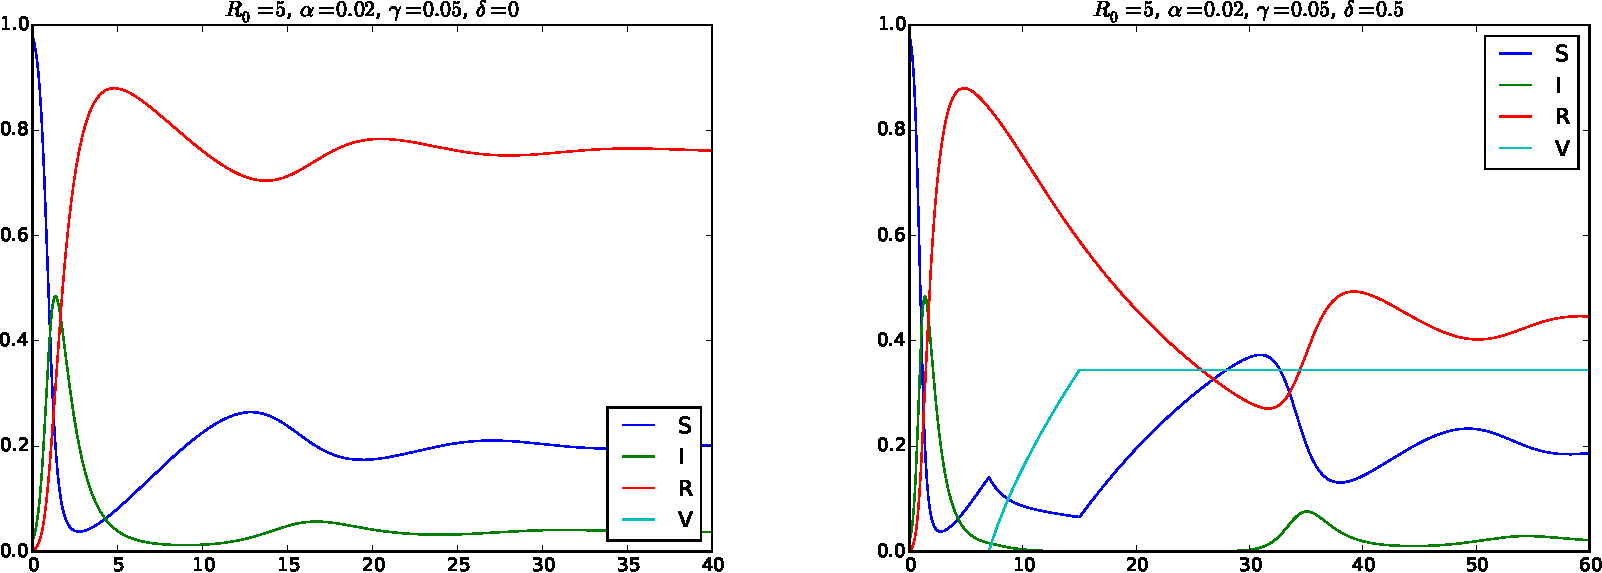
\includegraphics[width=1.0\linewidth]{fig-scaling/SIRV2.pdf}}
  \caption{
  Spreading of a disease with loss of immunity (left) and added vaccination (right). \label{sec:scale:SIRV:fig}
  }
\end{figure}
%\clearpage % flush figures sec:scale:SIRV:fig



\subsection{Michaelis-Menten kinetics for biochemical reactions}
\label{scale:MMK}

A classical reaction model in biochemistry describes how a
substrate S is turned into a product P with aid of an enzyme E.
S and E react to form a complex ES in the first stage of the reaction.
In the second stage, ES is turned into E and P.
Introducing the amount of S, E, ES, and P by $[S]$, $[E]$, $[ES]$, and
$[P]$, the mathematical model can be written as

\begin{align}
\frac{d[ES]}{dt} &= k_+[E][S] - k_v[ES] - k_-[ES],
\label{scale:MMK:ES1}\\ 
\frac{d[P]}{dt} &= k_v[ES],
\label{scale:MMK:P1}\\ 
\frac{d[S]}{dt} &= -k_+[E][S] + k_-[ES],
\label{scale:MMK:S1}\\ 
\frac{d[E]}{dt} &= -k_+[E][S] + k_-[ES] + k_v[ES]\tp
\label{scale:MMK:E1}
\end{align}
The initial conditions are $[ES](0)=[P](0)=0$, and $[S]=S_0$, $[E]=E_0$.
Three rate constants are involved: $k_+$, $k_-$, and $k_v$.
The above mathematical model is known as \href{{https://en.wikipedia.org/wiki/Michaelis-Menten_kinetics}}{Michaelis-Menten kinetics}\footnote{\texttt{https://en.wikipedia.org/wiki/Michaelis-Menten\_kinetics}}.

The amount of substance is measured in the unit \href{{https://en.wikipedia.org/wiki/Mole_(unit)}}{mole}\footnote{\texttt{https://en.wikipedia.org/wiki/Mole\_(unit)}} (mol). From the equations we can see that
$k_+$ is measured in $\hbox{s}^{-1}\hbox{mol}^{-1}$, while $k_-$ and
$k_v$ are measured in $\hbox{s}^{-1}$. It is convenient to get rid of
the mole unit for the amount of a substance. When working with
dimensionless quantities, only ratios of the rate constants and not their
specific values are needed.

\paragraph{Classical analysis.}
A common assumption is that the formation of $[ES]$ is very fast and that
it quickly reaches an equilibrium state, $[ES]^{\prime}=0$. Equation
(\ref{scale:MMK:ES1}) then reduces to the algebraic equation

\[ k_+[E][S] - k_v[ES] - k_-[ES] = 0, \]
which leads to

\begin{equation}
\frac{[E][S]}{[ES]} = \frac{k_- + k_v}{k_+} = K,
\label{scale:MMK:K}
\end{equation}
where $K$ is the famous Michaelis constant - the equilibrium constant
between $[E][S]$ and $[ES]$.

Another important observation is that the ODE system implies
two conservation equations, arising from simply adding the ODEs:

\begin{align}
\frac{d[ES]}{dt} + \frac{d[E]}{dt} & =0,\\ 
\frac{d[ES]}{dt} + \frac{d[S]}{dt} + \frac{d[P]}{dt} &= 0,
\end{align}
from which it follows that

\begin{align}
[ES] + [E] &= E_0,
\label{scale:MMK:cons1}\\ 
[ES] + [S] + [P] &= S_0\tp
\label{scale:MMK:cons2}
\end{align}

We can use (\ref{scale:MMK:cons1}) and (\ref{scale:MMK:K}) to
express $[E]$ by $[S]$:

\[ [E] = E_0 - [ES] = E_0 - \frac{[E][S]}{K}\quad\Rightarrow\quad
[E] = \frac{KE_0}{K + [S]}\tp\]
Now (\ref{scale:MMK:S1}) can be developed to an equation involving
$[S]$ only:

\begin{align}
\frac{d[S]}{dt} &= -k_+[E][S] + k_-[ES]\nonumber\\ 
& = (-k_+ + \frac{k_-}{K})[E][S]\nonumber\\ 
& = (-k_+ + \frac{k_-}{K})[S]\frac{KE_0}{K + [S]}\nonumber\\ 
& = - \frac{k_-E_0}{[S] + K}\tp
\label{scale:MMK:Seq1}
\end{align}
We see that the parameter $K$ is central.

From above expression for $[E]$ and (\ref{scale:MMK:cons1}) it now follows

\[
[E]=\frac{K E_0}{K+[S]},\quad [ES]=\frac{E_0[S]}{K+[S]}.
\]
If $K$ is comparable to $S_0$ these indicate

\[
[E]\sim E_0,\quad [ES]\sim \frac{E_0 S_0}{K},
\]
as is used for scaling $[E]$ and $Q_c$, subsequently.
Provided we exclude the case $[S]\gg K$, we may infer that $[E]$ will be of magnitude $E_0$, while $[ES]$ will be of magnitude $E_0 S_0/K$.

\paragraph{Dimensionless ODE system.}
Let us reason how to make the original ODE system
(\ref{scale:MMK:ES1})-(\ref{scale:MMK:E1}) dimensionless.
Aiming at $[S]$ and $[E]$ of unit size, two obvious dimensionless
unknowns are

\[ \bar S = \frac{[S]}{S_0},\quad
\bar E = \frac{[E]}{E_0}\tp\]
For the other two unknowns we just introduce scales to be determined
later:

\[
\bar P = \frac{[P]}{P_c},\quad
\bar{Q} = \frac{[ES]}{Q_c}\tp
\]
With $\bar t = t/t_c$ the equations become

\begin{align*}
\frac{d\bar Q}{d\bar t} &= t_ck_+\frac{E_0S_0}{Q_c}\bar E\bar S
- t_c(k_v + k_-)\bar Q,\\ 
\frac{d\bar P}{d\bar t} &= t_ck_v\frac{Q_c}{P_c}\bar Q,\\ 
\frac{d\bar S}{d\bar t} &= -t_ck_+E_0\bar E\bar S
+ t_ck_-\frac{Q_c}{S_0}\bar Q,\\ 
\frac{d\bar E}{d\bar t} &= -t_ck_+S_0\bar E\bar S
+ t_c(k_- + k_v)\frac{Q_c}{E_0}\bar Q\tp
\end{align*}
% \href{{http://www.biosym.uzh.ch/modules/models/Michaelis_Menten/michaelis_menten.html}}{\nolinkurl{http://www.biosym.uzh.ch/modules/models/Michaelis_Menten/michaelis_menten.html}}
% \href{{http://deepblue.lib.umich.edu/bitstream/handle/2027.42/26960/0000527.pdf}}{\nolinkurl{http://deepblue.lib.umich.edu/bitstream/handle/2027.42/26960/0000527.pdf}}?sequence=1
% \href{{http://www.math.ubc.ca/~keshet/EnzKin.pdf}}{\nolinkurl{http://www.math.ubc.ca/~keshet/EnzKin.pdf}}
% Good (but complicated): \href{{https://people.maths.ox.ac.uk/maini/PKM%20publications/9.pdf}}{\nolinkurl{https://people.maths.ox.ac.uk/maini/PKM\%20publications/9.pdf}}
% \href{{http://www.ncbi.nlm.nih.gov/pmc/articles/PMC2932968/}}{\nolinkurl{http://www.ncbi.nlm.nih.gov/pmc/articles/PMC2932968/}} (read this one - it is the best, this one has units for the constants too and typical values of constants)
% Murray has S_c=S_0, Q_c=E_0 (that is common)
% All use the long time scale with E_0
% Murray has much complicated analysis before selecting scales...
% Can find Q_c from Q'=0 which gives Q_c=E_0S_0/K

\paragraph{Determining scales.}
Choosing the scales is actually a quite complicated matter that requires
extensive analysis of the equations to determine the characteristics of
the solutions. Much literature is written about this, but here we shall
take a simplistic and pragmatic approach.
Besides the Michaelis constant $K$, there is another important parameter,

\[ \epsilon = \frac{E_0}{S_0},\]
because most applications will involve a small $\epsilon$.
We shall have $K$ and $\epsilon$ in mind while choosing scales such that
these symbols appear naturally in the scaled equations.

Looking at the equations, we see that the $K$ parameter will appear
if $t_c\sim 1/k_+$. However, $1/k_+$ does not have the dimension
$\hbox{[T]}^{-1}$ as required, so we need to add a factor with dimension
mol. A natural choice is
$t_c^{-1}=k_+S_0$ or $t_c^{-1}=k_+E_0$. Since often $S_0\gg E_0$,
the former $t_c$ is a short time scale and the latter is a long
time scale. If the interest is in the long time scale, we set

\[ t_c = \frac{1}{k_+E_0}\tp\]
The equations then take the form

\begin{align*}
\frac{d\bar Q}{d\bar t} &= \frac{S_0}{Q_c}\bar E\bar S
- KE_0^{-1}\bar Q,\\ 
\frac{d\bar P}{d\bar t} &= \frac{k_v}{k_+ E_0}\frac{Q_c}{P_c}\bar Q,\\ 
\frac{d\bar S}{d\bar t} &= -\bar E\bar S
+ \frac{k_-}{k_+E_0}\frac{Q_c}{S_0}\bar Q,\\ 
\frac{d\bar E}{d\bar t} &= -\epsilon^{-1}\bar E\bar S
+ K\frac{Q_c}{E_0^2}\bar Q\tp
\end{align*}
The $[ES]$ variable starts and ends at zero, and its maximum value
can be roughly estimated from the equation for $[ES]^\prime$
by setting $[ES]^\prime = 0$, which gives

\[ [ES] = \frac{[E][S]}{K}\sim \frac{E_0S_0}{K},\]
where we have replaced $[E][S]$ by $E_0S_0$ as an identification
of magnitude. This magnitude of $[ES]$
at its maximum can be used as the characteristic size $Q_c$:

\[ Q_c = \frac{E_0S_0}{K}\tp\]

The equation for $\bar P$ simplifies if we choose $P_c=Q_c$.
With these assumptions one gets

\begin{align*}
\frac{d\bar Q}{d\bar t} &= KE_0^{-1} (\bar E\bar S
- \bar Q),\\ 
\frac{d\bar P}{d\bar t} &= \frac{k_v}{k_+ E_0}\bar Q,\\ 
\frac{d\bar S}{d\bar t} &= -\bar E\bar S
+ \frac{k_-}{k_+E_0}\frac{E_0}{K}\bar Q,\\ 
\frac{d\bar E}{d\bar t} &= -\epsilon^{-1}\bar E\bar S
+ \epsilon^{-1}\bar Q\tp
\end{align*}
We can now identify the dimensionless numbers

\[ \alpha = \frac{K}{E_0},\quad \beta = \frac{k_v}{k_+ E_0},
\quad \gamma = \frac{k_-}{k_+E_0},
\]
where we see that $\alpha = \beta + \gamma$, so $\gamma$ can be eliminated.
Moreover,

\[ \alpha = \frac{k_-}{k_+E_0} + \beta,\]
implying that $\alpha > \beta$.

We arrive at the final set of scaled differential equations:

\begin{align}
\frac{d\bar Q}{d\bar t} &= \alpha (\bar E\bar S
- \bar Q),
\label{scale:MMK:Q2}\\ 
\frac{d\bar P}{d\bar t} &= \beta\bar Q,
\label{scale:MMK:P2}\\ 
\frac{d\bar S}{d\bar t} &= -\bar E\bar S
+ (1 - \beta\alpha^{-1})\bar Q,
\label{scale:MMK:S2}\\ 
\epsilon\frac{d\bar E}{d\bar t} &= -\bar E\bar S + \bar Q\tp
\label{scale:MMK:E2}
\end{align}
The initial conditions are $\bar S=\bar E =1$ and $\bar Q=\bar P=0$.

The five initial parameters ($S_0$, $E_0$, $k_+$, $k_-$, and $k_v$)
are reduced to three dimensionless constants:

\begin{itemize}
 \item $\alpha$ is the dimensionless Michaelis constant, reflecting the
   ratio of the production of P and E ($k_v+k_-$) versus the production of
   the complex ($k_+$), made dimensionless by $E_0$,

 \item $\epsilon$ is the initial fraction of enzyme relative to the substrate,

 \item $\beta$ measures the relative importance of production of P ($k_v$)
   versus production of the complex ($k_+$), made dimensionless by $E_0$.
\end{itemize}

\noindent
Observe that software developed for
solving (\ref{scale:MMK:ES1})-(\ref{scale:MMK:E1}) cannot be reused
for solving (\ref{scale:MMK:Q2})-(\ref{scale:MMK:E2}) since the latter
system has a slightly different structure.

\paragraph{Conservation equations.}
The counterpart to the conservation equations
(\ref{scale:MMK:cons1})-(\ref{scale:MMK:cons2}) is obtained by
adding (\ref{scale:MMK:Q2}) and $\alpha$ times (\ref{scale:MMK:E2}),
and adding (\ref{scale:MMK:Q2}), (\ref{scale:MMK:P2}), and
$\alpha$ times (\ref{scale:MMK:S2}):

\begin{align}
\epsilon^{-1}\alpha^{-1}\bar Q + \bar E &= 1,\\ 
\alpha\bar S + \bar Q + \bar P &= \alpha\tp
\end{align}

The scaled quantities, as well as the original concentrations, must be
positive variables, and $\bar E\in [0,1]$, $\bar S\in [0,1]$. Such checks
along with the conserved quantities above should be performed at every
time step in a simulation.

\paragraph{Analysis of the scaled system.}
In the scaled system, we may assume $\epsilon$ small, which from
(\ref{scale:MMK:E2}) gives rise to the simplification
$\epsilon\bar E^{\prime}=0$, and thereby the relation $\bar Q = \bar E\bar S$.
The conservation equation $[ES] + [E]= E_0$ reads $Q_c\bar Q + E_0\bar E =
E_0$ such that $\bar E = 1 - Q_c\bar Q/E_0=1- \bar Q S_0/K = 1 - \epsilon^{-1}\alpha^{-1}\bar Q$. The relation $\bar Q=\bar E\bar S$ then becomes

\[ \bar Q = (1 - \epsilon^{-1}\alpha^{-1}\bar Q)\bar S,\]
which can be solved for $\bar Q$:

\[ \bar Q = \frac{\bar S}{1 + \epsilon^{-1}\alpha^{-1}\bar S}\tp\]
The equation (\ref{scale:MMK:S2}) for $\bar S$ becomes

\begin{equation}
\frac{d\bar S}{d\bar t} = -\beta\alpha^{-1}\bar Q =
-\frac{\beta\bar S}{\alpha + \epsilon^{-1}\bar S}\tp
\label{scale:MMK:Seq2}
\end{equation}
This is a more precise analysis than the one leading to
(\ref{scale:MMK:Seq1}) since we now realize that the
mathematical assumption for the simplification is
$\epsilon\rightarrow 0$.

Is (\ref{scale:MMK:Seq2}) consistent with (\ref{scale:MMK:Seq1})? It is
easy to make algebraic mistakes when deriving scaled equations,
so it is always wise to carry out consistency checks.
Introducing dimensions in (\ref{scale:MMK:Seq2}) leads to

\[
\frac{t_c}{S_0}\frac{d S}{dt} =
\frac{d\bar S}{d\bar t}  =
-\frac{\beta\bar S}{\alpha + \epsilon^{-1}\bar S}
= -\frac{k_v}{k_+E_0}\frac{S}{KE_0^{-1} + E_0^{-1}S_0\bar S}
= -\frac{k_v}{k_+}\frac{\bar S}{K + S},\]
and hence with $t_c^{-1}=k_+E_0$,

\[ \frac{dS}{dt} = -\frac{k_vE_0 S}{K + S},\]
which is (\ref{scale:MMK:Seq1}).

Figure~\ref{scale:MMK:fig} shows the impact of $\epsilon$: with a moderately small
value (0.1) we see that $\bar Q\approx 0$, which justifies the
simplifications performed above. We also observe that all the unknowns
vary between 0 and about 1, indicating that the scaling is successful
for the chosen dimensionless numbers. The simulations made use of
a time step $\Delta\bar t=0.01$ with a 4th-order Runge-Kutta method,
using $\alpha=1.5$, $\beta=1$ (relevant code is in the
\Verb!simulate_biochemical_process! function in \href{{http://tinyurl.com/o8pb3yy/session.py}}{\nolinkurl{session.py}}).


\begin{figure}[!ht]  % scale:MMK:fig
  \centerline{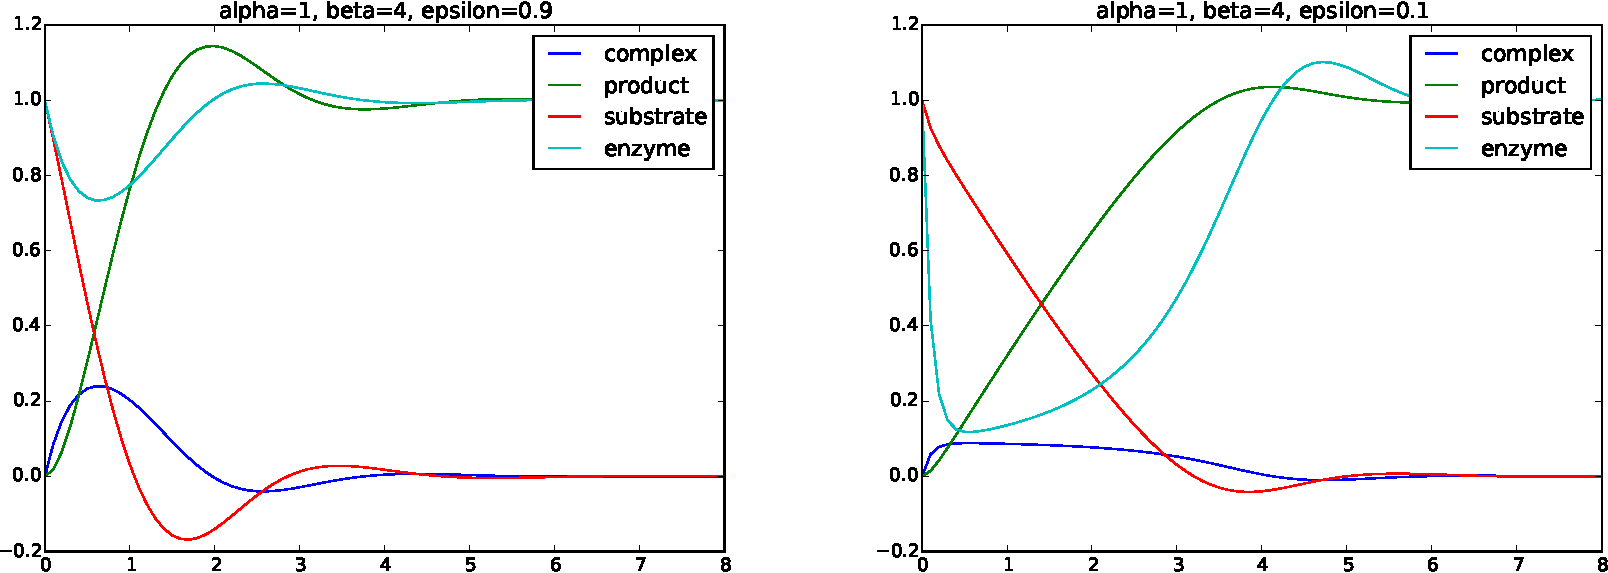
\includegraphics[width=1.0\linewidth]{fig-scaling/biochem.pdf}}
  \caption{
  Simulation of a biochemical process. \label{scale:MMK:fig}
  }
\end{figure}
%\clearpage % flush figures scale:MMK:fig


However, it is of interest to investigate the limit $\epsilon\rightarrow 0$.
Initially, the equation for $d\bar E/d\bar t$ reads
$d\bar E/d\bar t = -\epsilon^{-1}$, which implies a very fast reduction of
$\bar E$. Using $\epsilon=0.005$ and $\Delta\bar t = 10^{-3}$, simulation
results show that $\bar E$ decays to approximately zero at $t=0.03$ while
$\bar S\approx 1$ and $\bar Q \approx \bar P\approx 0$.
This is reasonable since with
very little enzyme in comparison with the substrate ($\epsilon\rightarrow 0$)
very little will happen.

% !split
\section{Vibration problems}
\label{sec:scale:vib}

We shall in this section
address a range of different second-order ODEs for mechanical
vibrations and demonstrate how to reason about the scaling in
different physical scenarios.


\subsection{Undamped vibrations without forcing}
\label{sec:scale:vib:undamped}

The simplest differential equation model for mechanical vibrations
reads

\begin{equation}
mu'' + ku = 0,\quad u(0)=I,\ u'(0)=V,
\label{sec:scale:vib:undamped:model}
\end{equation}
where unknown $u(t)$ measures the displacement of the body,
This is a common model for a vibrating body  with mass $m$ attached
to a linear spring with spring constant $k$ (and force $-ku$).
Figure~\ref{sec:scale:vib:undamped:sketch} shows a typical mechanical
sketch of such a system: some mass can move horizontally without friction
and is connected to a spring that exerts a force $-ku$ on the body.


\begin{figure}[!ht]  % sec:scale:vib:undamped:sketch
  \centerline{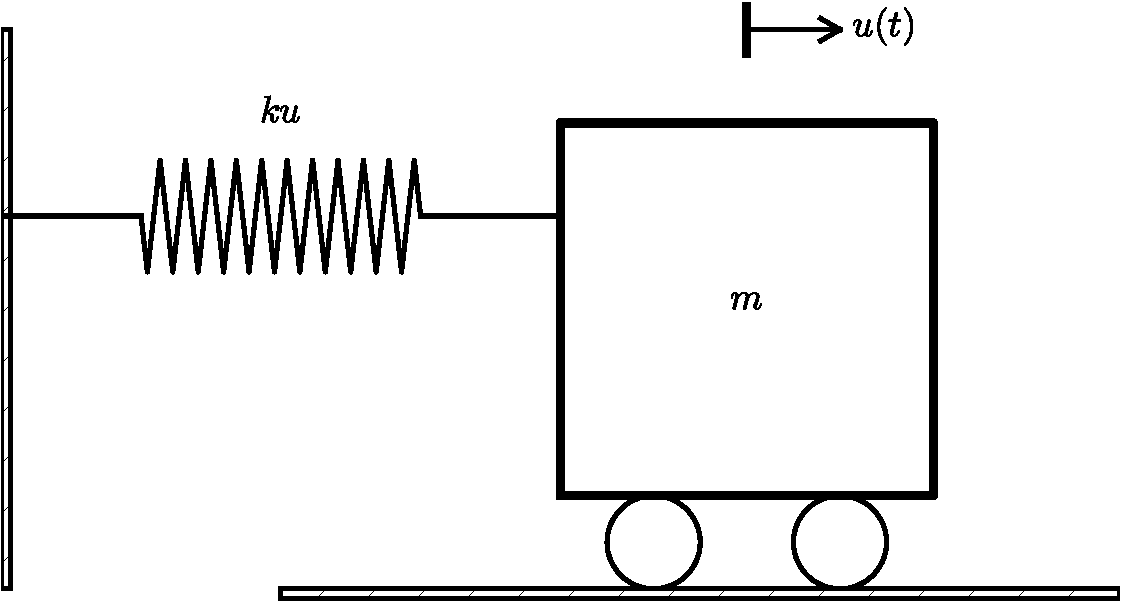
\includegraphics[width=0.6\linewidth]{fig-scaling/oscillator_spring.pdf}}
  \caption{
  Oscillating body attached to a spring. \label{sec:scale:vib:undamped:sketch}
  }
\end{figure}
%\clearpage % flush figures sec:scale:vib:undamped:sketch


\paragraph{The first technical steps of scaling.}
The problem (\ref{sec:scale:vib:undamped:model}) has one independent
variable $t$ and one dependent variable $u$. We introduce dimensionless
versions of these variables:

\[ \bar u =\frac{u}{u_c},\quad\bar t = \frac{t}{t_c},\]
where $u_c$ and $t_c$ are characteristic values of $u$ and $t$.
Inserted in (\ref{sec:scale:vib:undamped:model}), we get

\[ m\frac{u_c}{t_c^2}\frac{d^2\bar u}{d\bar t^2} + ku_c\bar u = 0,
\quad u_c\bar u(0)=I,\quad \frac{u_c}{t_c}\frac{d\bar u}{d\bar t}(0)=V,\]
resulting in

\begin{equation}
\frac{d^2\bar u}{d\bar t^2} + \frac{t_c^2 k}{m}\bar u = 0,
\quad \bar u(0)=\frac{I}{u_c},\ \bar u'(0)=\frac{Vt_c}{u_c}\tp
\label{sec:scale:vib:undamped:model:scaled0}
\end{equation}

What is an appropriate displacement scale $u_c$? The initial condition
$u(0)=I$ is a candidate, i.e., $u_c=I$. But how to choose the time scale?
Making the coefficient in front of the $\bar u$ unity, such that
both terms balance and are of size unity, is a candidate.

\paragraph{The exact solution.}
To better see what the proper scales of $u$ and $t$ are, we can look
into the analytical solution of this problem.
Although the exact solution of
(\ref{sec:scale:vib:undamped:model}) is quite straightforward to calculate
by hand, we take the opportunity to make use of SymPy to
find $u(t)$. The use of SymPy can later be generalized to vibration
ODEs that are harder to solve by hand.

SymPy requires all mathematical symbols to be explicitly created:

\begin{lstlisting}[language=Python,style=graycolor]
from sympy import *
u = symbols('u', cls=Function)
w = symbols('w', real=True, positive=True)
I, V, C1, C2 = symbols('I V C1 C2', real=True)
\end{lstlisting}
To specify the ODE to be solved, we can make a Python function returning
all the terms in the ODE:

\begin{lstlisting}[language=Python,style=graycolor]
# Define differential equation: u'' + w**2*u = 0
def ode(u):
    return diff(u, t, t) + w**2*u

diffeq = ode(u(t))
\end{lstlisting}
The \texttt{diffeq} variable, defining the ODE, can be passed to the SymPy
function \texttt{dsolve} to find the symbolic solution of the ODE:

\begin{lstlisting}[language=Python,style=graycolor]
s = dsolve(diffeq, u(t))
# s is an u(t) == expression (Eq obj.), s.rhs grabs the expression
u_sol = s.rhs
print u_sol
\end{lstlisting}
The solution that gets printed is \texttt{C1*sin(t*w) + C2*cos(t*w)}, indicating
that there are two integration constants \texttt{C1} and \texttt{C2} to be determined
by the initial conditions. The result of applying these conditions is
a $2\times 2$ linear system of algebraic equations that SymPy can solve
by the \texttt{solve} function. The code goes as follows:

\begin{lstlisting}[language=Python,style=graycolor]
# The solution u_sol contains integration constants C1 and C2
# but these are not symbols, substitute them by symbols
u_sol = u_sol.subs('C1', C1).subs('C2', C2)

# Determine C1 and C2 from the initial conditions
ic = [u_sol.subs(t, 0) - I, u_sol.diff(t).subs(t, 0) - V]
print ic   # 2x2 algebraic system for C1 and C2
s = solve(ic, [C1, C2])
# s is now a dictionary: {C2: I, C1: V/w}
# substitute solution back in u_sol
u_sol = u_sol.subs(C1, s[C1]).subs(C2, s[C2])
print u_sol
\end{lstlisting}
The \Verb!u_sol! variable is now \texttt{I*cos(t*w) + V*sin(t*w)/w}.
Since symbolic software is far from bug-free and can give wrong results,
we should always check the answer. Here, we insert the solution in the ODE
to see if the result is zero, and we insert the solution in the initial
conditions to see that these are fulfilled:

\begin{lstlisting}[language=Python,style=graycolor]
# Check that the solution fulfills the ODE and init.cond.
print simplify(ode(u_sol)),
print u_sol.subs(t, 0) - I, diff(u_sol, t).subs(t, 0) - V
\end{lstlisting}
There will be many more examples on using SymPy to find exact solutions
of differential equation problems.

The solution of the ODE in mathematical notation is

\[ u(t) = I\cos(\omega t) + \frac{V}{\omega}\sin(\omega t),\quad \omega = \sqrt{\frac{k}{m}}\tp\]
More insight arises from rewriting such an expression in the form
$A\cos(wt - \phi)$:

\[ u(t) = \sqrt{I^2 + \frac{V^2}{\omega^2}}\cos(wt - \phi),\quad
\phi = \tan^{-1}(V/(\omega I))\tp
\]
Now we see that the $u$ corresponds to cosine oscillations with a
frequency shift $\phi$ and amplitude $\sqrt{I^2 + (V/\omega)^2}$.


\paragraph{Discussion of the displacement scale.}
The amplitude of $u$ is $\sqrt{I^2 + V^2/\omega^2}$, and this
expression is obviously a candidate for $u_c$.  However, the simpler
choice $u_c=\max (I, V/\omega)$ is also relevant and more attractive
than the square root expression (but potentially a factor 1.4 wrong
compared to the exact amplitude).  It is not very important to have
$|u|\leq 1$, the point is to avoid $|u|$ very small or large.

\paragraph{Discussion of the time scale.}
What is an appropriate time scale? Looking at
(\ref{sec:scale:vib:undamped:model:scaled0}) and arguing that
$\bar u''$ and $\bar u$ both should be around unity in size, the
coefficient $t_c^2k/m$ must equal unity, implying that $t_c=\sqrt{m/k}$.
Also from the analytical solution we see that the solution goes like the
sine or cosine of $\omega t$, so $1/\omega = \sqrt{m/k}$ can be a characteristic
time scale. Likewise, one period of the oscillations, $P=2\pi/\omega$, can
be the characteristic time, leading to $t_c=2\pi/\omega$.

\paragraph{The dimensionless solution.}
With $u_c=I$ and $t_c=\sqrt{m/k}$ we get the scaled model

\begin{equation}
\frac{d^2\bar u}{d\bar t^2} + \bar u = 0,
\quad \bar u(0)=1,\ \bar u'(0)=\alpha,
\label{sec:scale:vib:undamped:model:scaled1}
\end{equation}
where $\alpha$ is a dimensionless parameter:

\[ \alpha = \frac{V}{I}\sqrt{\frac{m}{k}}\tp\]
Note that in case $V=0$, we have ``scaled away'' all physical parameters.
The universal solution without physical parameters is then
$\bar u(\bar t)=\cos\bar t$.

The unscaled solution is recovered as

\begin{equation}
u(t) = I\bar u(\sqrt{k/m}\bar t)\tp
\end{equation}
This expressions shows that the scaling is simply a matter of
\emph{stretching or shrinking the axes}.

\paragraph{Alternative displacement scale.}
Using $u_c = V/\omega$, the equation
is not changed, but the initial conditions become

\[ \bar u(0) = \frac{I}{u_c} = \frac{I\omega}{V} =\frac{I}{V}\sqrt{\frac{k}{m}} = \alpha^{-1},\quad \bar u'(0)=1\tp\]


With $u_c=V/\omega$ and one period as time scale,
$t_c=2\pi\sqrt{m/k}$,
we get the alternative model

\begin{equation}
\frac{d^2\bar u}{d\bar t^2} + 4\pi^2 \bar u = 0,
\quad \bar u(0)=\alpha^{-1},\ \bar u'(0)=2\pi\tp
\label{sec:scale:vib:undamped:model:scaled2}
\end{equation}
The unscaled solution is in this case recovered by

\begin{equation}
u(t) = V\sqrt{\frac{m}{k}}\bar u(2\pi\sqrt{k/m}\bar t)\tp
\end{equation}

\index{frequency}
\index{frequency, angular}
\index{period (of oscillations)}
\index{radians}
\index{angular frequency}

\paragraph{About frequency and dimensions.}
The solution goes like $\cos\omega t$, where $\omega =\sqrt{m/k}$
must have dimension 1/s. Actually, $\omega$ has dimension \emph{radians
per second}: rad/s. A radian is dimensionless since it is arc (length)
divided by radius (length), but still regarded as a unit.
The period $P$ of vibrations is a more intuitive quantity than the frequency
$\omega$. The relation between $P$ and $\omega$ is $P=2\pi/\omega$.
The number of oscillation cycles per period, $f$, is a more intuitive
measurement of frequency and also known as \emph{frequency}. Therefore, to be
precise, $\omega$ should be named \emph{angular frequency}. The relation between
$f$ and $T$ is $f=1/T$, so $f=2\pi\omega$ and measured in Hz (1/s), which is
the unit for counts per unit time.

\subsection{Undamped vibrations with constant forcing}
\label{sec:scale:vib:undamped:mg}

For vertical vibrations in the gravity field, the model
(\ref{sec:scale:vib:undamped:model}) must also take the gravity force
$-mg$ into account:

\[ mu'' + ku = -mg\tp\]
How does the new term $-mg$ influence
the scaling? We observe that if there is no movement of the body,
$u''=0$, and the spring elongation matches the gravity force:
$ku = -mg$, leading to a steady displacement $u=-mg/k$. We can then
have oscillations around this equilibrium point. A natural scaling
for $u$ is therefore

\[ \bar u = \frac{u - (-mg/k)}{u_c}=\frac{uk + mg}{ku_c}\tp\]
% u = - mg/k + u_c\bar u
The scaled differential equation with the same time scale as before
reads

\[ \frac{d^2\bar u}{d\bar t^2} + \bar u - \frac{t_c^2}{u_c}g
= -\frac{t_c^2}{u_c}g,\]
leading to

\[ \frac{d^2\bar u}{d\bar t^2} + \bar u = 0\tp\]
The initial conditions $u(0)=I$ and $u'(0)=V$ become, with $u_c=I$,

\[ \bar u(0) = 1 + \frac{mg}{kI},\quad \frac{d\bar u}{d\bar t}(0)=\sqrt{\frac{m}{k}}\frac{V}{I}\tp\]
We see that the oscillations around the equilibrium point in the
gravity field are identical to the horizontal oscillations without
gravity, except for an offset $mg/(kI)$ in the displacement.


\subsection{Undamped vibrations with time-dependent forcing}
\label{sec:scale:vib:undamped:F}

Now we add a transient forcing term $F(t)$ to the model
(\ref{sec:scale:vib:undamped:model}):

\begin{equation}
mu'' + ku = F(t),\quad u(0)=I,\ u'(0)=V\tp
\label{sec:scale:vib:undamped:F:model}
\end{equation}
Take the forcing to be oscillating:

\[ F(t) = A\cos(\psi t)\tp\]
The technical steps of the scaling are still the same, with the
intermediate result

\begin{equation}
\frac{d^2\bar u}{d\bar t^2} + \frac{t_c^2 k}{m}\bar u =
\frac{t_c^2}{mu_c}A\cos(\psi t_c\bar t),
\quad \bar u(0)=\frac{I}{u_c},\ \bar u'(0)=\frac{Vt_c}{u_c}\tp
\label{sec:scale:vib:undamped:F:model:scaled0}
\end{equation}
What are typical displacement and time scales? This is not so obvious
without knowing the details of the solution, because there are
three parameters ($I$, $V$, and $A$) that influence the magnitude of $u$.
Moreover, there are two time scales, one for the free vibrations of
the systems and one for the forced vibrations $F(t)$.

\paragraph{Investigating scales via analytical solutions.}
As we have seen already several times, having access to
an exact solution is very fortunate as it allows us to directly
examine the scales. Also in the present problem it is possible
to derive an exact solution. We
continue the SymPy session from the previous section and perform much
of the same steps. Note that we use \texttt{w} for $\omega = \sqrt{k/m}$
in the computer code (to obtain a more direct visual counterpart to
$\omega$).
SymPy may get confused when coefficients in differential equations
contain several symbols. We therefore rewrite the equation with
at most one symbol in each coefficient (i.e., symbolic software is
in general
more successful when applied to scaled differential equations than the
unscaled counterparts, but right now our task is to solve the unscaled version).
The amplitude $A/m$ in the forcing term is of this reason
replaced by the symbol \texttt{A1}.

\begin{lstlisting}[language=Python,style=graycolor]
A, A1, m, psi = symbols('A A1 m psi', positive=True, real=True)
def ode(u):
    return diff(u, t, t) + w**2*u - A1*cos(psi*t)

diffeq = ode(u(t))
u_sol = dsolve(diffeq, u(t))
u_sol = u_sol.rhs

# Determine the constants C1 and C2 in u_sol
# (first substitute our own declared C1 and C2 symbols,
# then use the initial conditions)
u_sol = u_sol.subs('C1', C1).subs('C2', C2)
eqs = [u_sol.subs(t, 0) - I, u_sol.diff(t).subs(t, 0) - V]
s = solve(eqs, [C1, C2])
u_sol = u_sol.subs(C1, s[C1]).subs(C2, s[C2])

# Check that the solution fulfills the equation and init.cond.
print simplify(ode(u_sol))
print simplify(u_sol.subs(t, 0) - I)
print simplify(diff(u_sol, t).subs(t, 0) - V)

u_sol = simplify(expand(u_sol.subs(A1, A/m)))
print u_sol
\end{lstlisting}
The output from the last line is

\begin{lstlisting}[language=Python,style=graycolor]
A/m*cos(psi*t)/(-psi**2 + w**2) + V*sin(t*w)/w +
(A/m + I*psi**2 - I*w**2)*cos(t*w)/(psi**2 - w**2)
\end{lstlisting}
With a bit of rewrite this expression becomes

% Note that the solution becomes a bit simpler of F is cos rather than sin

\[ u(t) = \frac{A/m}{\omega^2 - \psi^2}\cos(\psi t) + \frac{V}{\omega}
   \sin(\omega t) +
\left(\frac{A/m}{\psi^2 - \omega^2} + I\right) \cos (\omega t)\tp
\]
Obviously, this expression is only meaningful for $\psi\neq\omega$. The
case $\psi = \omega$ gives an infinite amplitude in this model, a
phenomenon known as resonance. The amplitude becomes finite when
damping is included,
see Section~\ref{sec:scale:vib:damped:F}.

When the system starts from rest, $I=V=0$, and the
forcing is the only driving mechanism, we can simplify:

\begin{align*}
u(t) &= \frac{A}{m(\omega^2 - \psi^2)}\cos(\psi t)
+
\frac{A}{m(\psi^2 - \omega^2)}\cos (\omega t)\\ 
&= \frac{A}{m(\omega^2 - \psi^2)}(\cos(\psi t) - \cos(\omega t))\tp
\end{align*}
To gain more insight, $\cos(\psi t) - \cos(\omega t)$ can be
rewritten in terms of the mean frequency $(\psi + \omega)/2$ and
the difference in frequency $(\psi - \omega)/2$:

\begin{equation}
u(t) = \frac{A}{m(\omega^2 - \psi^2)} 2
\sin\left(\frac{\psi - \omega}{2}t\right)
\sin\left(\frac{\psi + \omega}{2}t\right),
\label{sec:scale:vib:undamped:F:model:sinsin}
\end{equation}
showing that there is a signal with frequency $(\psi + \omega)/2$
whose amplitude has a (much) slower frequency
$(\psi - \omega)/2$. Figure~\ref{sec:scale:vib:fig:envelope} shows
an example on such a signal.



\begin{figure}[!ht]  % sec:scale:vib:fig:envelope
  \centerline{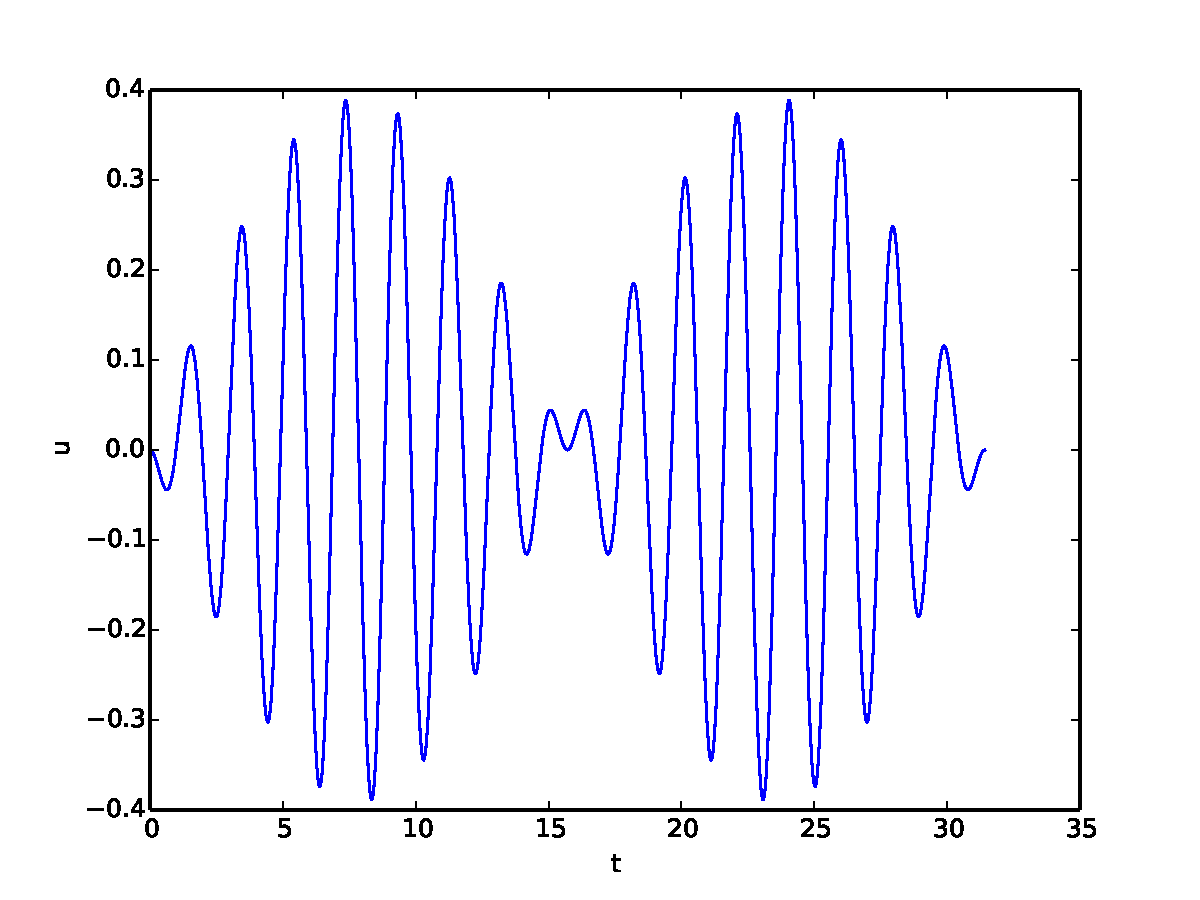
\includegraphics[width=0.8\linewidth]{fig-scaling/envelope.pdf}}
  \caption{
  Signal with frequency 3.1 and envelope frequency 0.2. \label{sec:scale:vib:fig:envelope}
  }
\end{figure}
%\clearpage % flush figures sec:scale:vib:fig:envelope



\paragraph{The displacement and time scales.}
A characteristic displacement can in the latter special case
be taken as $u_c= A/(m(\omega^2 - \psi^2))$. This is also a relevant choice
in the more general case $I\neq0, V\neq 0$, unless $I$ or $V$
is so large that it dominates over the amplitude
caused by the forcing. With $u_c= A/(m(\omega^2 - \psi^2))$ we also
have three special cases: $\omega \ll \psi$, $\omega \gg\psi$, and
$\psi \sim \omega$. In the latter case we need
$u_c= A/(m(\omega^2 - \psi^2))$ if we want $|u|\leq 1$. When
$\omega$ and $\psi$ are significantly different, we may choose one
of them and neglect the smaller. Choosing $\omega$ means $u_c=A/k$,
which is the relevant scale
if $\omega\gg\psi$. In the opposite case, $\omega\ll\psi$,
$u_c=A/(m\psi^2)$.

The time scale is dominated by the fastest oscillations, which are
of frequency $\psi$ or $\omega$ when these are close and the largest
of them when they are distant. In any case, we set
$t_c=1/\max(\psi,\omega)$.

\paragraph{Finding the displacement scale from the differential equation.}
Going back to (\ref{sec:scale:vib:undamped:F:model:scaled0}), we
may demand that all the three terms in the differential equation
are of size unity. This leads to $t_c=\sqrt{m/k}$
and $u_c=At_c^2/m = A/k$. The formula for $u_c$ is a kind of measure
of the ratio of the
forcing and the spring force (the dimensionless number
$A/(ku_c)$ would be this ratio).

Looking at (\ref{sec:scale:vib:undamped:F:model:sinsin}), we see
that if $\psi\ll\omega$, the amplitude can be approximated
by $A/(m\omega^2)=A/k$, showing that the scale $u_c=A/k$ is
relevant for an excitation frequency $\psi$ that is small compared to
the free vibration frequency $\omega$.

\paragraph{Scaling with free vibrations as time scale.}
The next step is to work out the dimensionless ODE for the chosen scales.
We first select the time scale based on the free oscillations
with frequency $\omega$, i.e., $t_c=1/\omega$. Inserting the expression in
(\ref{sec:scale:vib:undamped:F:model:scaled0}) results in

\begin{equation}
\frac{d^2\bar u}{d\bar t^2} + \bar u =
\gamma
\cos(\delta\bar t),
\quad \bar u(0)=\alpha,\ \bar u'(0)=\beta\tp
\label{sec:scale:vib:undamped:F:model:scaled2}
\end{equation}
Here we have four dimensionless variables

\begin{align}
\alpha &= \frac{I}{u_c},\\ 
\beta  &= \frac{Vt_c}{u_c} = \frac{V}{\omega u_c},\\ 
\gamma &= \frac{t_c^2 A}{mu_c} = \frac{A}{ku_c},\\ 
\delta &= \frac{t_c}{\psi^{-1}} = \frac{\psi}{\omega}\tp
\end{align}
We remark that the choice of $u_c$ has so far not been made. Several
different cases will be considered below, and we will see that certain
choices reduce the number of independent dimensionless variables to
three.

The four dimensionless variables above have interpretations as ratios of
physical effects:

\begin{itemize}
 \item $\alpha$: ratio of the initial displacement and
   the characteristic response $u_c$,

 \item $\beta$: ratio of the initial velocity
   and the typical velocity measure $u_c/t_c$,

 \item $\gamma$: ratio of
   the forcing $A$ and the mass times acceleration $mu_c/t_c^2$ \emph{or}
   the ratio of the forcing and the spring force $ku_c$

 \item $\delta$: ratio of the
   frequencies or the time scales of the forcing and the free vibrations.
\end{itemize}

\noindent
\paragraph{Software.}
Any solver for (\ref{sec:scale:vib:undamped:F:model:scaled0})
can be used for (\ref{sec:scale:vib:undamped:F:model:scaled2}).
More details are provided at the end of
Section~\ref{sec:scale:vib:damped:F}.

\paragraph{Choice of $u_c$ close to resonance.}
Now we shall discuss various choices of $u_c$.
Close to resonance, when $\psi\sim\omega$, we may set
$u_c=A/(m(\omega^2 - \psi^2))$. The dimensionless numbers
become in this case

\begin{align*}
\alpha &= \frac{I}{u_c} = \frac{I}{A/k}(1-\delta^2),\\ 
\beta  &= \frac{V}{\omega u_c} = \frac{V\sqrt{km}}{A}(1-\delta^2),\\ 
\gamma &= \frac{A}{ku_c} = 1-\delta^2,\\ 
\delta &= \frac{\psi}{\omega}\tp
\end{align*}
With $\psi = 0.99\omega$, $\delta =0.99$, $V=0$,
$\alpha = \gamma = 1-\delta^2 = 0.02$, we have the problem

\[
\frac{d^2\bar u}{d\bar t^2} + \bar u =
0.02 \cos(0.99\bar t),
\quad \bar u(0)=0.02,\ \bar u'(0)=0\tp
\]
This is a problem with a very small initial condition and a very small
forcing, but the state close to resonance brings the amplitude up to
about unity, see the result of numerical simulations with $\delta=0.99$ in
Figure~\ref{sec:scale:vib:fig:Fcos_b0:1}.
Neglecting $\alpha$,
the solution is given by (\ref{sec:scale:vib:undamped:F:model:sinsin}),
which here means $A=1-\delta^2$, $m=1$, $\omega=1$, $\psi=\delta$:

\[ \bar u(\bar t) = 2\sin(-0.005\bar t)\sin(0.995\bar t)\tp \]
Note that this is a problem which demands very high accuracy in the
numerical calculations. Using 20 time steps per period gives a
significant angular frequency error and an amplitude of about 1.4. We used
160 steps per period for the results in
Figure~\ref{sec:scale:vib:fig:Fcos_b0:1}.


\begin{figure}[!ht]  % sec:scale:vib:fig:Fcos_b0:1
  \centerline{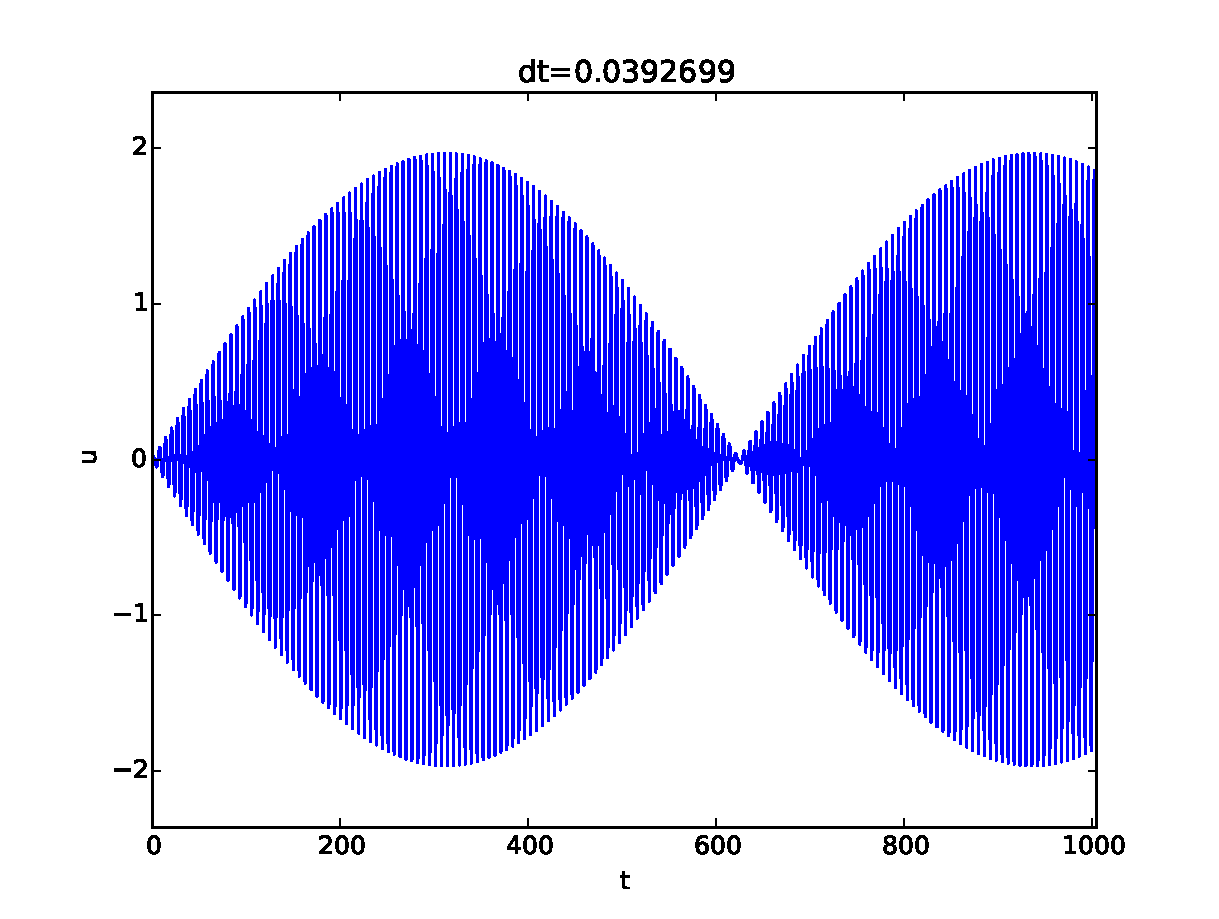
\includegraphics[width=1.0\linewidth]{fig-scaling/vib_delta099_b0_Fcos.pdf}}
  \caption{
  Forced undamped vibrations close to resonance. \label{sec:scale:vib:fig:Fcos_b0:1}
  }
\end{figure}
%\clearpage % flush figures sec:scale:vib:fig:Fcos_b0:1


\paragraph{Unit size of all terms in the ODE.}
Using the displacement scale $u_c=A/k$ leads to
(\ref{sec:scale:vib:undamped:F:model:scaled2}) with

\begin{align*}
\alpha &= \frac{I}{u_c} = \frac{I}{A/k},\\ 
\beta  &= \frac{V}{\omega u_c} = \frac{V k}{A\omega},\\ 
\gamma &= \frac{A}{ku_c} = 1,\\ 
\delta &= \frac{\psi}{\omega}\tp
\end{align*}
Simulating a case with $\delta=0.5$, $\alpha=1$, and $\beta=0$ gives
the oscillations in Figure~\ref{sec:scale:vib:fig:Fcos_b0:2}, which is
a case away from resonance, and the amplitude is about unity. However,
choosing $\delta =0.99$ (close to resonance) results in a figure
similar to Figure~\ref{sec:scale:vib:fig:Fcos_b0:1}, except that the
amplitude is about $10^2$ because of the moderate size of $u_c$.
The present scaling is therefore most suitable away from resonance,
and when the terms containing $\cos\omega t$ and $\sin\omega t$
are important (e.g., $\omega\gg\psi$).



\begin{figure}[!ht]  % sec:scale:vib:fig:Fcos_b0:2
  \centerline{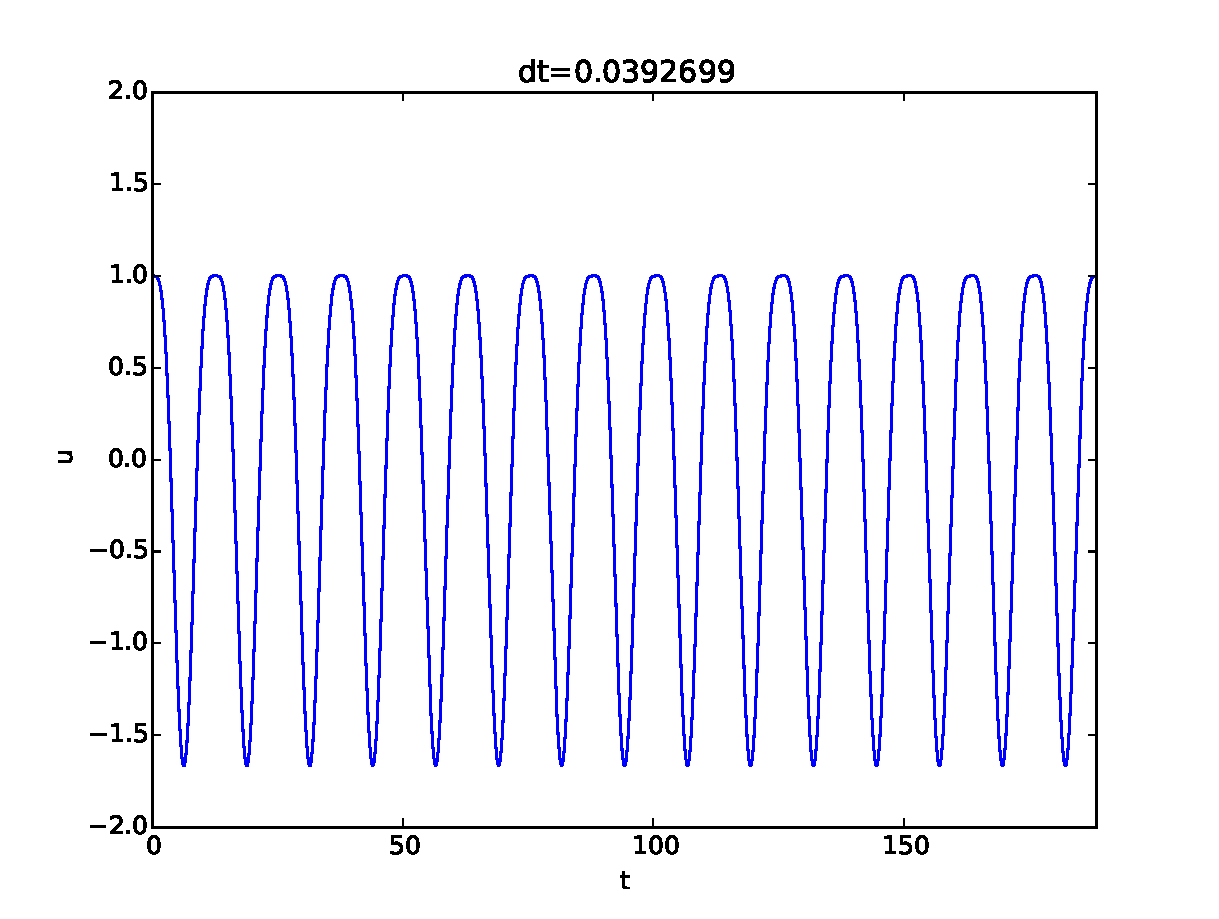
\includegraphics[width=1.0\linewidth]{fig-scaling/vib_delta05_b0_Fcos.pdf}}
  \caption{
  Forced undamped vibrations away from resonance. \label{sec:scale:vib:fig:Fcos_b0:2}
  }
\end{figure}
%\clearpage % flush figures sec:scale:vib:fig:Fcos_b0:2


\paragraph{Choice of $u_c$ when $\psi\gg\omega$.}
Finally, we may look at the case where $\psi\gg\omega$ such that
$u_c=A/(m\psi^2)$ is a relevant scale (i.e., omitting $\omega^2$ compared to
$\psi^2$ in the denominator), but in this case we should
use $t_c=1/\psi$ since the force varies much faster than the
free vibrations of the system.
This choice of $t_c$ changes the scaled ODE to

\begin{equation}
\frac{d^2\bar u}{d\bar t^2} + \delta^{-2}\bar u =
\gamma
\cos(\bar t),
\quad \bar u(0)=\alpha,\ \bar u'(0)=\beta,
\label{sec:scale:vib:undamped:F:model:scaled6}
\end{equation}
where

\begin{align*}
\alpha &= \frac{I}{u_c} = \frac{I}{A/k}\delta^2,\\ 
\beta  &= \frac{Vt_c}{u_c} = \frac{V\sqrt{km}}{A}\delta,\\ 
\gamma &= \frac{t_c^2 A}{mu_c} = 1,\\ 
\delta &= \frac{t_c}{\psi^{-1}} = \frac{\psi}{\omega}\tp
\end{align*}
In the regime $\psi\gg\omega$, $\delta\gg 1$, thus making $\alpha$ and
$\beta$ large.
However, if $\alpha$ and/or $\beta$ is large,
the initial condition dominates over the forcing, and will also dominate
the amplitude of $u$, thereby making the scaling of $u$ inappropriate.
In case $I=V=0$ so that $\alpha=\beta=0$,
(\ref{sec:scale:vib:undamped:F:model:sinsin}) predicts
($A=m=1$, $\omega=\delta^{-1}$, $\psi=1$)

\[ \bar u(\bar t) = (\delta^{-2}-1)^{-1}2
\sin\left(\frac{1}{2}(1 -\delta^{-1})\bar t\right)
\sin\left(\frac{1}{2}(1 +\delta^{-1})\bar t\right),
\]
which has an amplitude about $2$ for $\delta\gg 1$.
Figure~\ref{sec:scale:vib:fig:Fcos_b0:3} shows a case.



\begin{figure}[!ht]  % sec:scale:vib:fig:Fcos_b0:3
  \centerline{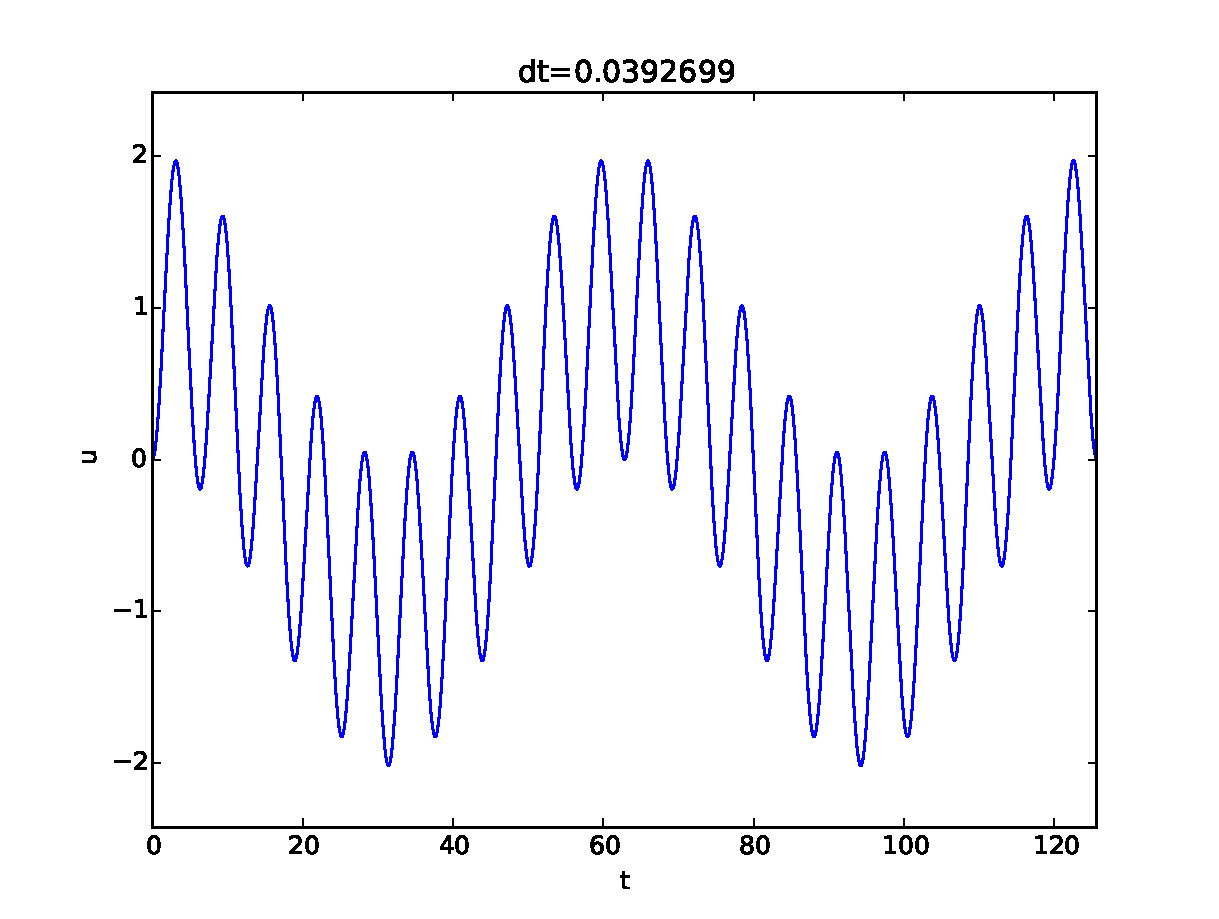
\includegraphics[width=1.0\linewidth]{fig-scaling/vib_delta10_b0_Fcos.pdf}}
  \caption{
  Forced undamped vibrations with rapid forcing. \label{sec:scale:vib:fig:Fcos_b0:3}
  }
\end{figure}
%\clearpage % flush figures sec:scale:vib:fig:Fcos_b0:3


With $\alpha=0.05\delta^2=5$, we get a significant contribution from
the free vibrations (the homogeneous solution of the ODE) as
shown in Figure~\ref{sec:scale:vib:fig:Fcos_b0:4}. For larger $\alpha$
values, one must base $u_c$ on $I$ instead.
(The graphs in Figure~\ref{sec:scale:vib:fig:Fcos_b0:3} and~\ref{sec:scale:vib:fig:Fcos_b0:4} were
produced by
numerical simulations with 160 time steps per period of the forcing.)


\begin{figure}[!ht]  % sec:scale:vib:fig:Fcos_b0:4
  \centerline{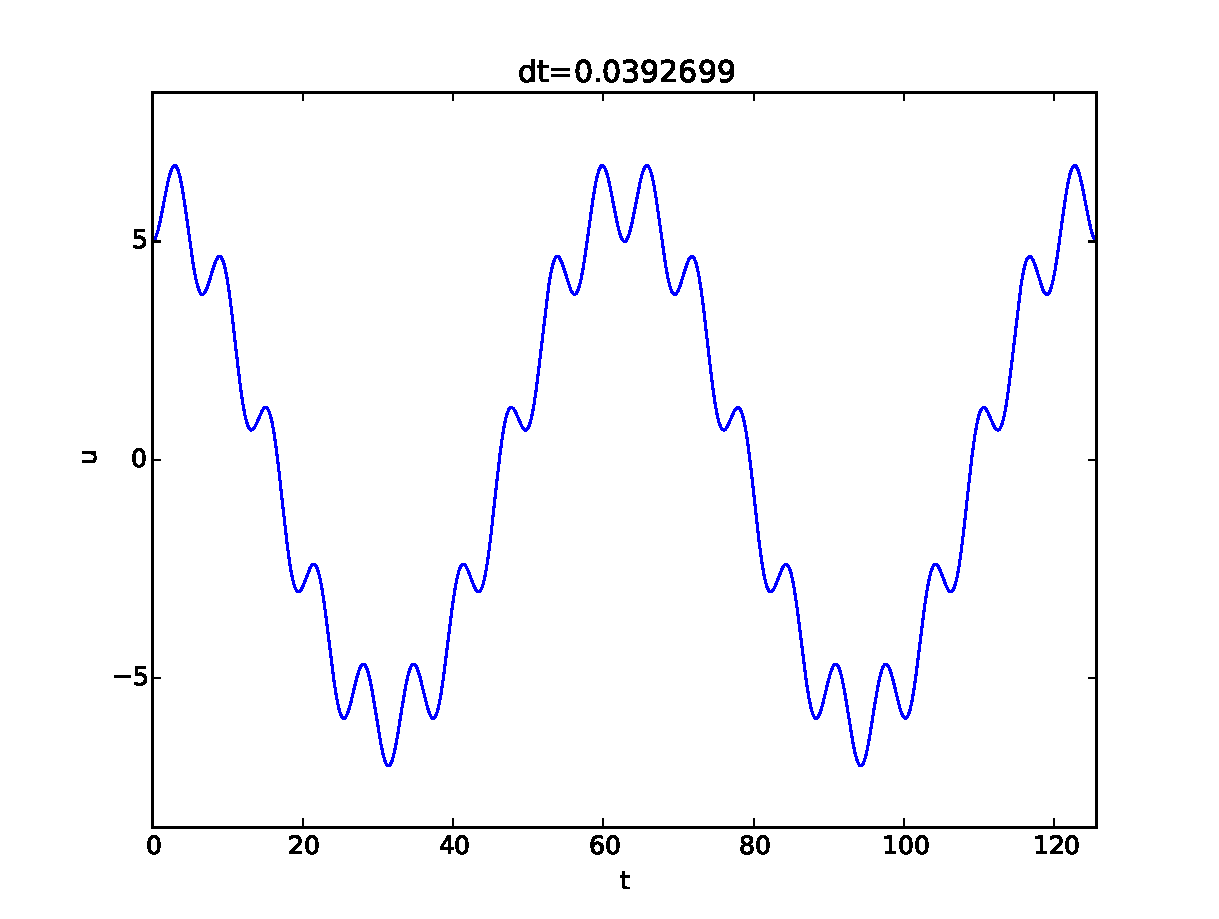
\includegraphics[width=1.0\linewidth]{fig-scaling/vib_delta10_b0_a5_Fcos.pdf}}
  \caption{
  Forced undamped vibrations with rapid forcing and initial displacement of 5. \label{sec:scale:vib:fig:Fcos_b0:4}
  }
\end{figure}
%\clearpage % flush figures sec:scale:vib:fig:Fcos_b0:4




\paragraph{Displacement scale based on $I$.}
Choosing $u_c=I$ gives

\begin{equation}
\frac{d^2\bar u}{d\bar t^2} + \bar u =
\gamma\cos(\delta\bar t),
\quad \bar u(0)=1,\ \bar u'(0)=\beta,
\label{sec:scale:vib:undamped:F:model:scaled5}
\end{equation}
with

\begin{align}
\beta  &= \frac{Vt_c}{u_c} = \frac{V}{I}\sqrt{\frac{m}{k}},\\ 
\gamma & = \frac{tc^2A}{mu_c} = \frac{A}{ku_c} = \frac{A}{kI} \tp
\end{align}
This scaling is not relevant close to resonance since then $u_c\gg I$.


\subsection{Damped vibrations with forcing}
\label{sec:scale:vib:damped:F}

We now introduce a linear damping force $bu'(t)$ in the equation of motion:

\begin{equation}
mu'' + bu' + ku = A\cos(\psi t),\quad u(0)=I,\ u'(0)=V\tp
\label{sec:scale:vib:damped:F:model}
\end{equation}
Figure~\ref{sec:scale:vib:damped:sketch} shows a typical
one-degree-of-freedom mechanical system with a linear dashpot, representing
the damper ($bu'$), a linear spring ($ku$), and an external force ($F$).


\begin{figure}[!ht]  % sec:scale:vib:damped:sketch
  \centerline{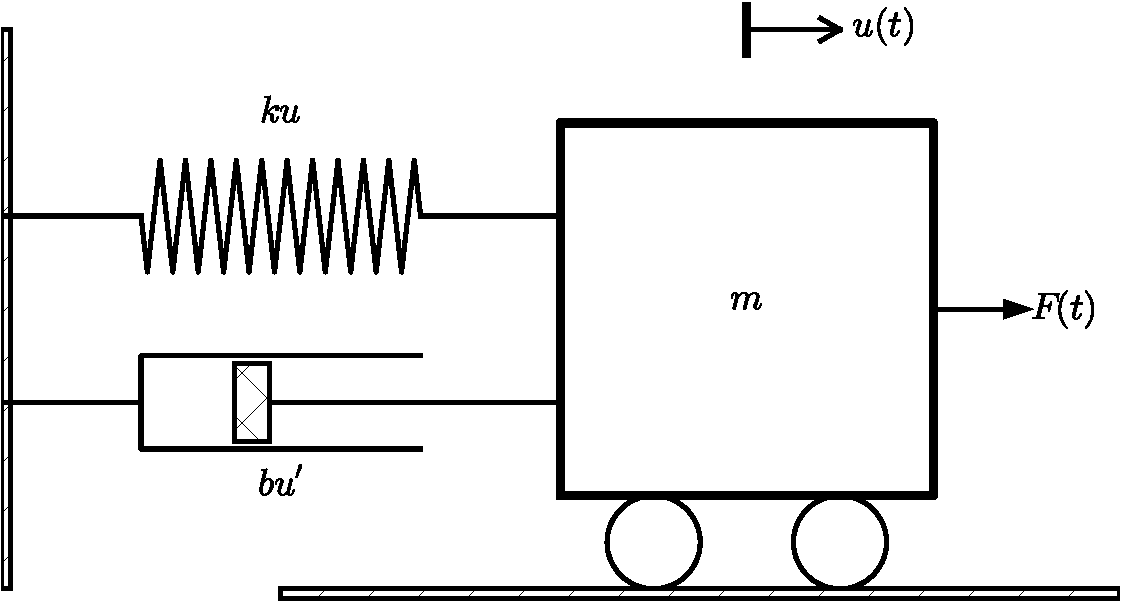
\includegraphics[width=0.6\linewidth]{fig-scaling/oscillator.pdf}}
  \caption{
  Oscillating body with external force, attached to a spring and damper. \label{sec:scale:vib:damped:sketch}
  }
\end{figure}
%\clearpage % flush figures sec:scale:vib:damped:sketch


The standard scaling procedure results in

\begin{equation}
\frac{d^2\bar u}{d\bar t^2} + \frac{t_c b}{m}\frac{d\bar u}{d\bar t}
+ \frac{t_c^2 k}{m}\bar u =
\frac{t_c^2}{mu_c}A\cos(\psi t_c\bar t),
\quad \bar u(0)=\frac{I}{u_c},\ \bar u'(0)=\frac{Vt_c}{u_c}\tp
\label{sec:scale:vib:damped:F:model:scaled0}
\end{equation}

\paragraph{The exact solution.}
As always, it is
a great advantage to look into exact solutions for controlling our
choice of scales.
Using SymPy to solve (\ref{sec:scale:vib:damped:F:model}) is, in principle,
very straightforward:

\begin{lstlisting}[language=Python,style=graycolor]
>>> diffeq = diff(u(t), t, t) + b/m*diff(u(t), t) + w**2*u(t)
>>> s = dsolve(diffeq, u(t))
>>> s.rhs
C1*exp(t*(-b - sqrt(b - 2*m*w)*sqrt(b + 2*m*w))/(2*m)) +
C2*exp(t*(-b + sqrt(b - 2*m*w)*sqrt(b + 2*m*w))/(2*m))
\end{lstlisting}
This is indeed the correct solution, but it is on a complex
exponential function form, valid for all $b$, $m$, and $\omega$. We are
interested in the case with \emph{small damping}, $b < 2m\omega$, where the solution
is an exponentially damped sinusoidal function. Rewriting the expression
in the right form is tricky with SymPy commands. Instead, we demonstrate
a common technique when doing symbolic computing: general procedures like
\texttt{dsolve} are replaced by manual steps. That is, we solve the ODE ``by hand'',
but use SymPy to assist the calculations.

The solution is composed of a homogeneous
solution $u_h$ of $mu'' + bu' + ku=0$ and one particular solution $u_p$
of the nonhomogeneous equation
$mu'' + bu' + ku=A\cos(\psi t)$. The homogeneous solution with
damped oscillations (requiring $b < 2\sqrt{mk}$) can be
found by the following code. We have divided the differential equation
by $m$ and introduced $B=\frac{1}{2}b/m$ and let \texttt{A1} represent
$A/m$ to simplify expressions and
help SymPy with less symbols in the equation. Without these simplifications,
SymPy stalls in the computations due to too many symbols in the equation.
The problem is actually a solid argument for scaling differential equations
before asking SymPy to solve them since scaling effectively reduces the
number of parameters in the equations!

The following SymPy steps derives the solution of the homogeneous ODE:

\begin{lstlisting}[language=Python,style=graycolor]
u = symbols('u', cls=Function)
t, w, B, A, A1, m, psi = symbols('t w B A A1 m psi',
                                 positive=True, real=True)

def ode(u, homogeneous=True):
    h = diff(u, t, t) + 2*B*diff(u, t) + w**2*u
    f = A1*cos(psi*t)
    return h if homogeneous else h - f

# Find coefficients in polynomial (in r) for exp(r*t) ansatz
r = symbols('r')
ansatz = exp(r*t)
poly = simplify(ode(ansatz)/ansatz)

# Convert to polynomial to extract coefficients
poly = Poly(poly, r)
# Extract coefficients in poly: a_*t**2 + b_*t + c_
a_, b_, c_ = poly.coeffs()
# Assume b_**2 - 4*a_*c_ < 0
d = -b_/(2*a_)
if a_ == 1:
    omega = sqrt(c_ - (b_/2)**2)  # nicer formula
else:
    omega = sqrt(4*a_*c_ - b_**2)/(2*a_)

# The homogeneous solution is a linear combination of a
# cos term (u1) and a sin term (u2)
u1 = exp(d*t)*cos(omega*t)
u2 = exp(d*t)*sin(omega*t)
C1, C2, V, I = symbols('C1 C2 V I', real=True)
u_h = simplify(C1*u1 + C2*u2)
print 'u_h:', u_h
\end{lstlisting}
The print out shows

\[ u_h = e^{-Bt}\left(C_1 \cos(\sqrt{\omega^2 - B^2}t) +
C_2 \sin(\sqrt{\omega^2 - B^2}t)\right),\]
where $C_1$ and $C_2$ must be determined by the initial conditions later.
It is wise to check that $u_h$ is indeed a solution of the homogeneous
differential equation:

\index{assert@{\rm\texttt{assert}}}

\begin{lstlisting}[language=Python,style=graycolor]
assert simplify(ode(u_h)) == 0
\end{lstlisting}
We have previously just printed the residuals of the ODE and initial
conditions after inserting the solution, but it is better in a code to
let the programming language test that the residuals are symbolically zero.
This is achieved using the \texttt{assert} statement in Python. The argument is
a boolean expression, and if the expression evaluates to \texttt{False},
an \texttt{AssertionError} is raised and the program aborts (otherwise \texttt{assert}
runs silently for a \texttt{True} boolean expression). Hereafter, we will use
\texttt{assert} for consistency checks in computer code.

The ansatz for the particular solution $u_p$ is

\[ u_p= C_3\cos(\psi t) + C_4\sin(\psi t),\]
which inserted in the ODE gives two equations
for $C_3$ and $C_4$. The relevant SymPy statements are

\begin{lstlisting}[language=Python,style=graycolor]
# Particular solution
C3, C4 = symbols('C3 C4')
u_p = C3*cos(psi*t) + C4*sin(psi*t)
eqs = simplify(ode(u_p, homogeneous=False))

# Collect cos(omega*t) terms
print 'eqs:', eqs
eq_cos = simplify(eqs.subs(sin(psi*t), 0).subs(cos(psi*t), 1))
eq_sin = simplify(eqs.subs(cos(psi*t), 0).subs(sin(psi*t), 1))
s = solve([eq_cos, eq_sin], [C3, C4])
u_p = simplify(u_p.subs(C3, s[C3]).subs(C4, s[C4]))

# Check that the solution is correct
assert simplify(ode(u_p, homogeneous=False)) == 0
\end{lstlisting}
Using the initial conditions for the complete solution $u=u_h+u_p$
determines $C_1$ and $C_2$:

\begin{lstlisting}[language=Python,style=graycolor]
u_sol = u_h + u_p  # total solution
# Initial conditions
eqs = [u_sol.subs(t, 0) - I, u_sol.diff(t).subs(t, 0) - V]
# Determine C1 and C2 from the initial conditions
s = solve(eqs, [C1, C2])
u_sol = u_sol.subs(C1, s[C1]).subs(C2, s[C2])
\end{lstlisting}
Finally, we should check that \Verb!u_sol! is indeed the correct solution:

\begin{lstlisting}[language=Python,style=graycolor]
checks = dict(
    ODE=simplify(expand(ode(u_sol, homogeneous=False))),
    IC1=simplify(u_sol.subs(t, 0) - I),
    IC2=simplify(diff(u_sol, t).subs(t, 0) - V))
for check in checks:
    msg = '%s residual: %s' % (check, checks[check])
    assert checks[check] == sympify(0), msg
\end{lstlisting}
Finally, we may take \Verb!u_sol = u_sol.subs(A, A/m)! to get the right
expression for the solution.
Using \Verb!latex(u_sol)! results in a huge expression, which should be
manually ordered to something like the following:

\begin{align*} u = &
\frac{Am^{-1}}{4 B^{2} \psi^{2} +
\Omega^{2}} \left(2 B \psi
\sin{\left (\psi t \right )} - \Omega\cos{\left (\psi t \right )}\right) + \\ 
&
{e^{-B t}} \biggl(
C_1 \cos{\left( t \sqrt{\omega^{2}- B^{2}}\right)} +
C_2 \sin{\left (t \sqrt{\omega^{2}- B^{2}}\right )}\biggr)\\ 
C_1 &= \frac{Am^{-1} \Omega + 4 I B^{2} \psi^{2} +
I\Omega^2}{
4 B^{2} \psi^{2} + \Omega^2}\\ 
C_2 &=
\frac{- Am^{-1} B\Omega + 4 I B^{3} \psi^{2} +
I B\Omega^2 + 4 V B^{2}\psi^{2} +
V\Omega^2}{
\sqrt{\omega^{2} - B^{2}}
\left(4 B^{2} \psi^{2} + \Omega^2\right)},\\ 
\Omega &= \psi^2 - \omega^2\tp
\end{align*}

\index{quality factor $Q$}
\index{phase shift}

The most important feature of this solution is that there are
two time scales with frequencies $\psi$ and $\sqrt{\omega^2 - B^2}$,
respectively,
but the latter appears in terms that decay as $e^{-Bt}$ in time.
The attention is usually on longer periods of time, so in that
case the solution simplifies to

\begin{align}
u &= \frac{Am^{-1}}{4 B^{2} \psi^{2} +
\Omega^{2}} \left(2 B \psi
\sin{\left (\psi t \right )} - \Omega\cos{\left (\psi t \right )}\right)
\nonumber\\ 
&= \frac{A}{m}\frac{1}{\sqrt{4B^2\psi^2 + \Omega^2}}\cos(\psi t + \phi)
\frac{(\psi\omega)^{-1}}{(\psi\omega)^{-1}}
\nonumber\\ 
& = \frac{A}{k} Q\delta^{-1}\left(1 + Q^2(\delta - \delta^{-1})\right)^{-
\frac{1}{2}}\cos(\psi t + \phi),
\label{sec:scale:vib:damped:F:model:u_forced0}
\end{align}
where we have introduced the dimensionless numbers

\[ Q = \frac{\omega}{2B},\quad\delta = \frac{\psi}{\omega},\]
and

\[ \phi = \tan^{-1}\left(-\frac{2B}{\omega^2 - \psi^2}\right)
= \tan^{-1}\left(\frac{Q^{-1}}{\delta^2 - 1}\right)\tp\]
$Q$ is commonly called \emph{quality factor} and $\phi$ is the
\emph{phase shift}. Dividing
(\ref{sec:scale:vib:damped:F:model:u_forced0}) by $A/k$, which is a common
scale for $u$, gives the dimensionless relation

\begin{equation}
\frac{u}{A/k} = \frac{Q}{\delta} R(Q,\delta)^{\frac{1}{2}}\cos(\psi t + \phi),
\quad
R(Q,\delta) = \left(1 + Q^2(\delta - \delta^{-1})\right)^{-1}\tp
\label{sec:scale:vib:damped:F:model:u_forced}
\end{equation}


\paragraph{Choosing scales.}
Much of the discussion about scales in the previous sections are
relevant also when damping is included.  Although the oscillations
with frequency $\sqrt{\omega^2-B^2}$ die out for $t\gg B^{-1}$, we
start with using this frequency for the time scale.  A highly relevant
assumption for engineering applications of
(\ref{sec:scale:vib:damped:F:model}) is that the damping is small.
Therefore, $\sqrt{\omega^2-B^2}$ is close to $\omega$ and we simply
apply $t_c=1/\omega$ as before (if not the interest in large $t$ for
which the oscillations with frequency $\omega$ has died out).

The coefficient in front of the $\bar u'$ term then becomes

\[ \frac{b}{m\omega} = \frac{2B}{\omega} = Q^{-1}\tp\]
The rest of the ODE is given in the previous section, and the particular
formulas depend on the choices of $t_c$ and $u_c$.

\paragraph{Choice of $u_c$ at resonance.}
The relevant scale for $u_c$ at or nearby resonance ($\psi = \omega$)
becomes different from the previous section, since with damping,
the maximum amplitude is a finite value. For $t\gg B^{-1}$, when the
$\sin\psi t$ term is dominating, we have for $\psi = \omega$:

\[ u = \frac{Am^{-1}2B\psi}{4B^2\psi^2}\sin (\psi t) =
\frac{A}{2Bm\psi}\sin (\psi t) =
\frac{A}{b\psi}\sin (\psi t)
\tp
\]
This motivates the choice

\[ u_c = \frac{A}{b\psi} = \frac{A}{b\omega}\tp\]
(It is wise during computations like this to stop and check the
dimensions: $A$ must be $[\hbox{MLT}^{-2}]$ from the original
equation ($F(t)$ must have the same dimension as $mu''$),
$bu'$ must also have dimension $[\hbox{MLT}^{-2}]$, implying that
$b$ has dimension $[\hbox{MT}^{-1}]$. $A/b$ then has dimension
$LT^{-1}$, and $A/(b\psi)$ gets dimension $[L]$, which matches
what we want for $u_c$.)

The differential equation on dimensionless form becomes

\begin{equation}
\frac{d^2\bar u}{d\bar t^2} + Q^{-1}\frac{d\bar u}{d\bar t} + \bar u =
\gamma
\cos(\delta\bar t),
\quad \bar u(0)=\alpha,\ \bar u'(0)=\beta,
\label{sec:scale:vib:damped:F:model:scaled1}
\end{equation}
with

% \frac{A}{b\omega}

\begin{align}
\alpha &= \frac{I}{u_c} = \frac{Ib}{A}\sqrt{\frac{k}{m}},\\ 
\beta  &= \frac{Vt_c}{u_c} = \frac{Vb}{A},\\ 
\gamma &= \frac{t_c^2 A}{mu_c} = \frac{b\omega}{k},\\ 
\delta &= \frac{t_c}{\psi^{-1}} = \frac{\psi}{\omega} = 1\tp
\end{align}

\paragraph{Choice of $u_c$ when $\omega\gg\psi$.}
In the limit $\omega\gg\psi$ and $t\gg B^{-1}$,

\[ u \approx \frac{A}{m\omega^2}\cos\psi t = \frac{A}{k}\cos\psi t,\]
showing that $u_c=A/k$ is an appropriate displacement scale.
(Alternatively, we get this scale also from demanding $\gamma=1$ in the ODE.)
The dimensionless numbers $\alpha$, $\beta$, and $\delta$ are as
for the forced vibrations without damping.

\paragraph{Choice of $u_c$ when $\omega\ll\psi$.}
In the limit $\omega\ll\psi$, we should base $t_c$ on the rapid
variations in the excitation: $t_c=1/\psi$.

\paragraph{Software.}
It is easy to reuse a solver for a general vibration problem also
in the dimensionless case.
In particular, we may use the \texttt{solver} function in the
file \href{{http://tinyurl.com/o8pb3yy/vib.py}}{\nolinkurl{vib.py}}:

\begin{lstlisting}[language=Python,style=graycolor]
def solver(I, V, m, b, s, F, dt, T, damping='linear'):
\end{lstlisting}
for solving the ODE problem

\[ mu'' + f(u') + s(u) = F(t),\quad u(0)=I,\ u'(0)=V,\ t\in (0,T],\]
with time steps \texttt{dt}. With \texttt{damping='linear'}, we have $f(u')=bu'$, while the
other value is \texttt{'quadratic'}, meaning $f(u')=b|u'|u'$.
Given the dimensionless numbers $\alpha$, $\beta$, $\gamma$, $\delta$,
and $Q$,
an appropriate call for solving (\ref{sec:scale:vib:undamped:F:model:scaled2}) is

\begin{lstlisting}[language=Python,style=graycolor]
u, t = solver(I=alpha, V=beta, m=1, b=1.0/Q,
              s=lambda u: u, F=lambda t: gamma*cos(delta*t),
	      dt=2*pi/n, T=2*pi*P)
\end{lstlisting}
where \texttt{n} is the number of intervals per period and \texttt{P} is the number
of periods to be simulated.
We way wrap this call in a \Verb!solver_scaled! function and wrap it furthermore
with \texttt{joblib} to avoid repeated calls,
as we explained in
Section~\ref{sec:scale:prog}:

\begin{lstlisting}[language=Python,style=graycolor]
from vib import solver as solver_unscaled

def solver_scaled(alpha, beta, gamma, delta, Q, T, dt):
    """
    Solve u'' + (1/Q)*u' + u = gamma*cos(delta*t),
    u(0)=alpha, u'(1)=beta, for (0,T] with step dt.
    """
    print 'Computing the numerical solution'
    from math import cos
    return solver_unscaled(I=alpha, V=beta, m=1, b=1./Q,
                           s=lambda u: u,
                           F=lambda t: gamma*cos(delta*t),
                           dt=dt, T=T, damping='linear')

import joblib
disk_memory = joblib.Memory(cachedir='temp')
solver_scaled = disk_memory.cache(solver_scaled)
\end{lstlisting}
This code is found in \href{{http://tinyurl.com/o8pb3yy/vib_scaled.py}}{\nolinkurl{vib_scaled.py}}
and features an application for running the scaled problem with
options on the command-line for $\alpha$, $\beta$, $\gamma$, $\delta$,
$Q$, number of time steps per period, and number of periods (see
the \texttt{main} function). It is an ideal application for exploring
scaled vibration models.


\subsection{Oscillating electric circuits}

The differential equation for an oscillating electric circuit is
very similar to the equation for forced, damped,
mechanical vibrations, and their
dimensionless form is identical. This fact will now be demonstrated.

The current $I(t)$ in a
circuit having an inductor with inductance $L$, a capacitor with
capacitance $C$, and overall resistance $R$, obeys the equation

\begin{equation}
\ddot I + \frac{R}{L}\dot I + \frac{1}{LC}I =  V(t),
\end{equation}
where $V(t)$ is the voltage source powering the circuit.
We introduce

\[ \bar I=\frac{I}{I_c},\quad \bar t = \frac{t}{t_c},\]
and get

\[ \frac{d^2\bar I}{d\bar t^2} + \frac{t_c R}{L}\frac{d\bar I}{d\bar t}
+ \frac{t_c^2}{LC}\bar I = \frac{t_c^2V_c}{I_c} \bar V(t)\tp\]
Here, we have scaled $V(t)$ according to

\[ \bar V(\bar t) = \frac{V(t_c\bar t)}{\max_t V(t)}\tp\]

The time scale $t_c$ is chosen to make $\ddot I$ and $I/(LC)$ balance,
$t_c = \sqrt{LC}$.
Choosing $I_c$ to make the coefficient in the source term of unit size,
means $I_c = LCV_c$.
With

\[ Q^{-1} = R\sqrt{\frac{C}{L}},\]
we get the scaled equation

\begin{equation}
\frac{d^2\bar I}{d\bar t^2} + Q^{-1}\frac{d\bar I}{d\bar t}
+ \bar I = \bar V(t),
\end{equation}
which is basically the same as we derived for mechanical vibrations.
(Two additional dimensionless variables will arise from the initial
conditions for $I$, just as in the mechanics cases.)


% !split
\chapter{Basic partial differential equation models}

This chapter extends the scaling technique to well-known partial differential
equation (PDE) models for waves, diffusion, and transport.
We start out with the simplest 1D models of the PDEs and then progress
with additional terms, different types of boundary and initial conditions,
and generalizations to 2D and 3D.

\section{The wave equation}
\label{sec:scale:wave}

A standard, linear, one-dimensional wave equation problem
in a homogeneous medium may be written as

\begin{equation}
\frac{\partial^2 u}{\partial t^2} =
c^2 {\partial^2 u\over\partial x^2}, \quad  x\in (0,L),\ t\in (0,T],
\label{scale:wave:pde1}
\end{equation}
where $c$ is the constant wave velocity of the medium.
With a briefer notation, where subscripts indicate derivatives,
the PDE (\ref{scale:wave:pde1}) can be written
$u_{tt}=c^2u_{xx}$. This subscript notation will occasionally be
used later.

For any number of dimensions in heterogeneous media we have the generalization

\begin{equation}
\frac{\partial^2 u}{\partial t^2} =
\nabla\cdot\left(c^2 \nabla u\right) + f, \quad  x,y,z\in \Omega,\ t\in (0,T],
\label{scale:wave:pde1:3D}
\end{equation}
where $f$ represents a forcing.
% How to scale time depends on the PDE, the spatial scale depends on
% the domain, and the scale of $u$ usually depends on $f$ or the
% boundary or initial condition.

\subsection{Homogeneous Dirichlet conditions in 1D}
\label{sec:scale:wave:bc_u0}

Let us first start with (\ref{scale:wave:pde1}),
homogeneous Dirichlet conditions in space, and
no initial velocity $u_t$:

\begin{align}
u(x,0) &= I(x), \quad &x\in [0,L],
\label{scale:wave:pde1:ic:u}\\ 
{\partial\over\partial t}u(x,0) &= 0, \quad & x\in [0,L],
\label{scale:wave:pde1:ic:ut}\\ 
u(0,t) & = 0, \quad  & t\in (0,T],
\label{scale:wave:pde1:bc:0}\\ 
u(L,t) & = 0, \quad  & t\in (0,T].
\label{scale:wave:pde1:bc:L}
\end{align}
The independent variables are $x$ and $t$, while $u$ is the dependent
variable.
The rest of the parameters, $c$, $L$, $T$, and $I(x)$, are given data.

We start with introducing dimensionless versions of the independent and
dependent variables:

\[
\bar x = \frac{x}{x_c},\quad \bar t=\frac{t}{t_c},\quad\bar u=\frac{u}{u_c}
\tp
\]
Inserting the $x=x_c\bar x$, etc., in (\ref{scale:wave:pde1}) and
(\ref{scale:wave:pde1:ic:u})-(\ref{scale:wave:pde1:bc:L}) gives

\begin{align*}
\frac{\partial^2 \bar u}{\partial \bar t^2} &=
\frac{t_c^2c^2}{x_c^2}{\partial^2 \bar u\over\partial x^2}, \quad & \bar x\in (0,L/x_c),\ \bar t\in (0,T/t_c],
\\ 
\bar u(\bar x,0) &= \frac{I(x_c\bar x)}{u_c},
\quad &\bar x\in [0,L/x_c],
\\ 
\frac{\partial}{\partial \bar t}\bar u(\bar x,0) &= 0,
\quad & \bar x\in [0,L/x_c],
\\ 
\bar u(0,\bar t) & = 0,
\quad  & \bar t\in (0,T/t_c],
\\ 
\bar u(L/x_c,\bar t) & = 0,
\quad &\bar t\in (0,T/t_c].
\end{align*}

The key question is how to define the scales.
A natural choice is $x_c=L$ since this makes $\bar x\in [0,1]$.
For the spatial scale and the problem governed by
(\ref{scale:wave:pde1}) we
have some analytical insight that can help.
The solution behaves like

\begin{equation}
u(x,t) = f_R(x-ct) + f_R(x+ct),
\label{scale:wave:pde:sol:general}
\end{equation}
i.e., a right- and left-going wave with velocity $c$. The initial
conditions constrain the choices of $f_R$ and $f_L$ to $f_L + f_R=I$
and $-cf_L' + cf_R' = 0$. The solution is $f_R = f_L = \frac{1}{2}$,
and consequently

\[
u(x,t) = \frac{1}{2}I(x-ct) + \frac{1}{2}I(x+ct),
\]
which tells that the initial condition splits in two, half of it moves
to the left and half to the right.
This means in particular that we can choose $u_c=\max_x |I(x)|$
and get $|\bar u|\leq 1$, which is a goal. It must be added that
boundary conditions may result in reflected waves, and the solution is
then more complicated than indicated in the formula above.

Regarding the time scale, we may look at the two terms in the scaled
PDE and argue that if $|u|$ and its derivatives are to be of order unity,
then the size of the second-order derivatives should be the same, and
$t_c$ can be chosen to make the coefficient $t_c^2 c^2 /x_c^2$ unity,
i.e., $t_c=L/c$.
Another reasoning may set $t_c$ as the time it takes the wave
to travel through the domain $[0,L]$. Since the wave has constant
speed $c$, $t_c = L/c$.

With the described choices of scales,
we end up with the dimensionless initial-boundary value problem

\begin{align}
\frac{\partial^2 \bar u}{\partial \bar t^2} &=
{\partial^2 \bar u\over\partial x^2}, \quad & \bar x\in (0,1),\ \bar t\in (0,\bar T],
\label{scale:wave:pde1:d}\\ 
\bar u(\bar x,0) &= \frac{I(\bar x L)}{\max_{x\in(0,L)} |I(x)|},
\quad &\bar x\in [0,1],
\label{scale:wave:pde1:ic:u:d}\\ 
{\partial\over\partial \bar t}\bar u(\bar x,0) &= 0,
\quad & \bar x\in [0,1],
\label{scale:wave:pde1:ic:ut:d}\\ 
\bar u(0,\bar t) & = 0,
\quad  &\bar t\in (0,\bar T],
\label{scale:wave:pde1:bc:0:d}\\ 
\bar u(1,\bar t) & = 0,
\quad  &\bar t\in (0,\bar T].
\label{scale:wave:pde1:bc:L:d}
\end{align}
Here, $\bar T = Tc/L$.

The striking feature of
(\ref{scale:wave:pde1:d})-(\ref{scale:wave:pde1:bc:L:d})
is that there are \emph{no physical parameters} involved! Everything we need
to specify is the shape of the initial condition and then scale it
such that it is less than or equal to 1.

The physical solution with dimension is recovered from $\bar u(\bar x,\bar t)$
through

\begin{equation}
u(x,t) = \max_{x\in(0,L)}I(x)\,\bar u(\bar x L, \bar t L/c)
\end{equation}

\subsection{Implementation of the scaled wave equation}
\label{sec:scale:wave:impl}

How do we implement (\ref{scale:wave:pde1:d})-(\ref{scale:wave:pde1:bc:L:d})?
As for the simpler mathematical models, we suggest to implement the model
with dimensions and observe how to set parameters to obtain the scaled
model. In the present case, one must choose $L=1$, $c=1$, and scale $I$ by its
maximum value. That's all!

Several implementations of 1D wave equation models with different
degree of mathematical and software complexity come along with these
notes. The simplest
version is \href{{http://tinyurl.com/o8pb3yy/wave1D_u0.py}}{\nolinkurl{wave1D_u0.py}}
that implements (\ref{scale:wave:pde1}) and
(\ref{scale:wave:pde1:ic:u})-(\ref{scale:wave:pde1:bc:L}).
This is the code to be used in the following. It is described
in Section~\ref{wave:pde1:impl} in \cite{Langtangen_Linge_fdm}.


\paragraph{Waves on a string.}
As an example, we may let the original initial-boundary value problem
(\ref{scale:wave:pde1})-(\ref{scale:wave:pde1:bc:L}) model vibrations of
a string on a string instrument (e.g., a guitar).
With $u$ as the displacement of the
string, the boundary conditions $u=0$ at the ends are relevant, as
well as the zero velocity condition $\partial u/\partial t=0$ at
$t=0$.  The initial condition $I(x)$ typically has a triangular shape
for a picked guitar string.  The physical problem needs parameters for
the amplitude of $I(x)$, the length $L$ of the string, and the value
of $c$ for the string. Only the latter is challenging as it involves
relating $c$ to the pitch (i.e., time frequency) of the string. In the
scaled problem, we can forget about all this. We simply set $L=1$,
$c=1$, and let $I(x)$ have a peak of unity at $x=x_0\in(0,1)$:

\[
\frac{I(x)}{\max_x I(x)} = \left\lbrace
\begin{array}{ll}
x/x_0, & x < x_0,\\ 
(1-x)/(1-x_0), & \hbox{otherwise}
\end{array}\right.
\]
The dimensionless coordinate of the peak, $x_0$, is the only
dimensionless parameter in the problem. For fixed $x_0$,
one single simulation will capture all possible solutions with such
an initial triangular shape.


\paragraph{Detecting an already computed case.}
The file \href{{http://tinyurl.com/o8pb3yy/wave1D_u0_scaled.py}}{\nolinkurl{wave1D_u0_scaled.py}}
has functionality for detecting whether a simulation corresponds to
a previously run scaled case, and if so, the solution is retrieved from
file. The implementation technique makes use of \texttt{joblib}, but is more
complicated than shown previously in these notes since some of the
arguments to the function that computes the solution are functions,
and one must recognized if the function has been used as argument
before or not. There is documentation in the \Verb!wave1D_u0_scaled.py!
file explaining how this is done.


\subsection{Time-dependent Dirichlet condition}
\label{scale:wave:pde2}

A generalization of (\ref{scale:wave:pde1})-(\ref{scale:wave:pde1:bc:L})
is to allow for a time-dependent Dirichlet condition at one end, say
$u(0,t)=U_L(t)$. At the other end we may still have $u=0$.  This new
condition at $x=0$ may model a specified wave that enters the
domain. For example, if we feed in a monochromatic wave
$A\sin(k(x-ct))$ from the left end, $U_L(t)=A\sin (kct)$.  This
forcing of the wave motion has its own amplitude and time scale that
could affect the choice of $u_c$ and $t_c$.

The main difference from the previous initial-boundary value problem
is the condition at $x=0$, which now reads

\[ \bar u(0,\bar t) = \frac{U_L(\bar t t_c)}{u_c}\]
in scaled form.

\paragraph{Scaling.}
Regarding the characteristic time scale, it is natural to base this
scale on the wave propagation velocity, together with the length
scale, and not on the time scale of $U_L(t)$, because the time scale
of $U_L$ basically determines whether short or long waves are fed in
at the boundary. All waves, long or short, propagate with the same
velocity $c$. We therefore continue to use $t_c=L/c$.

The solution $u$ will have one wave contribution from the initial
condition $I$ and one from the feeding of waves at $x=0$. This gives
us three choices of $u_c$: $\max_x |I| + \max_t |U_L|$, $\max_x |I|$,
or $\max_t |U_L|$. The first seems relevant if the size of $I$ and
$U_L$ are about the same, but then we can choose either $\max_x |I|$
or $\max_t |U_L|$ as characteristic size of $u$ since a factor of 2 is
not important. If $I$ is much less than $U_L$, $u_c=\max_t |u_L|$ is
relevant, while $u_c=\max_x|I|$ is the choice when $I$ has much bigger
impact than $U_L$ on $u$.

With $u_c=\max_t |U_L(t)|$, we get the scaled problem

\begin{align}
\frac{\partial^2 \bar u}{\partial \bar t^2} &=
{\partial^2 \bar u\over\partial \bar x^2},
\quad & \bar x\in (0,1),\ \bar t\in (0,\bar T],
\label{scale:wave:pde2:d}\\ 
\bar u(\bar x,0) &= \frac{I(x_c\bar x)}{\max_t |U_L(t)|},
\quad &\bar x\in [0,1],
\label{scale:wave:pde2:ic:u:d}\\ 
{\partial\over\partial \bar t}\bar u(\bar x,0) &= 0,
\quad & \bar x\in [0,1],
\label{scale:wave:pde2:ic:ut:d}\\ 
\bar u(0,\bar t) & = \frac{U_L(\bar tt_c)}{\max_t |U_L(t)|},
\quad  &\bar t\in (0,\bar T],
\label{scale:wave:pde2:bc:0:d}\\ 
\bar u(1,\bar t) & = 0,
\quad &\bar t\in (0,\bar T].
\label{scale:wave:pde2:bc:L:d}
\end{align}
Also this problem is free of physical parameters like $c$ and $L$.
The input is completely specified by the shape of $I(x)$ and $U_L(t)$.

\paragraph{Software.}
Software for the original problem with dimensions can be reused for
(\ref{scale:wave:pde2:d})-(\ref{scale:wave:pde2:bc:L:d}) by
setting $L=1$, $c=1$, and scaling $U_L(t)$ and $I(x)$ by
$\max_t |U_L(t)|$.

\paragraph{Specific case.}
As an example, consider

\begin{align*}
U_L(t) &= a\sin(\omega t)\hbox{ for } 0\leq t\leq 2\frac{\omega}{2\pi},
\hbox{ else } 0,\\ 
I(x)   & = Ae^{-(x-L/2)^2/\sigma^2}\tp
\end{align*}
That is, we start with a Gaussian peak-shaped wave in the center of the
domain and feed in a sinusoidal wave at the left end for two periods.
The solution will be the sum of three waves: two parts from the initial
condition, plus the wave fed in from the left.

Since $\max_t |U_L|=a$ we get

\begin{align}
\bar u(\bar x,0) &= \frac{A}{a}e^{-(L/\sigma)^2(\bar x -\frac{1}{2})^2},
\label{scale:wave:oscbc:I}\\ 
\bar u(0,\bar t) &= \sin(\bar t\omega L/c)\tp
\label{scale:wave:oscbc:u0}
\end{align}
Here, $U_L$ models an incoming wave $a\sin(k(x-ct)$, with $k$ specified.
The result is incoming
waves of length $\lambda = 2\pi/k$. Since $\omega =kc$,
$\bar u(0,\bar t)=\sin(kL\bar t) = \sin(2\pi\bar t L/\lambda)$.
(This formula demonstrates the previous assertion that the time scale
of $U_L$, i.e., $1/\omega$, determines the wave length $1/\omega = \lambda/(2\pi)$ in space.)
We realize from the formulas (\ref{scale:wave:oscbc:I}) and
(\ref{scale:wave:oscbc:u0})
that there are three key dimensionless parameters related
to these specific choices of initial and boundary conditions:

\[ \alpha = \frac{A}{a},\quad\beta = \frac{L}{\sigma},\quad\gamma = kL
=2\pi\frac{L}{\lambda}\tp\]
With $\alpha$, $\beta$, and $\gamma$ we can write the dimensionless
initial and boundary conditions as

\begin{align*}
\bar u(\bar x,0) &= \alpha e^{-\beta^2(\bar x -\frac{1}{2})^2},\\ 
\bar u(0,\bar t) &= \sin(\gamma\bar t)\tp
\end{align*}
The dimensionless parameters have the following interpretations:

\begin{itemize}
 \item $\alpha$: ratio of initial condition amplitude and amplitude of incoming wave
   at $x=0$

 \item $\beta$: ratio of length of domain and width of initial condition

 \item $\gamma$: ratio of length of domain and wave length of incoming wave
\end{itemize}

\noindent
Again, these dimensionless parameters tell a lot about the interplay of
the physical effects in the problem. And only some ratios count!

We can simulate two special cases:

\begin{enumerate}
\item $\alpha=10$ (large) where the
   incoming wave is small and the solution is dominated by the two waves
   arising from $I(x)$,

\item $\alpha=0.1$ (small) where the incoming waves
   dominate and the solution has the initial condition just
   as a small perturbation of the wave shape.
\end{enumerate}

\noindent
We may choose a peak-shaped initial condition: $\beta = 10$,
and also a relatively short incoming wave compared to the domain size:
$\gamma = 6\pi$ (i.e., wave length of incoming wave is $L/6$).
A function \Verb!simulate_Gaussian_and_incoming_wave! in
the file \href{{http://tinyurl.com/o8pb3yy/session.py}}{\nolinkurl{session.py}}
applies the general unscaled
solver in \href{{http://tinyurl.com/o8pb3yy/wave1D_dn.py}}{\nolinkurl{wave1D_dn.py}}
for solving the wave equation with constant $c$,
and any time-dependent function or $\partial u/\partial x=0$ at the
end points. This solver is trivially adapted to the present case.
% @@@CODE src-scaling/session.py fromto: def simulate_Gaussian_and@import odespy
Figures~\ref{scale:wave:pde2:fig:alpha10} and~\ref{scale:wave:pde2:fig:alpha01}
shows snapshots of how $\bar u(\bar x,\bar t)$ evolves due to a
large/small initial condition and small/large incoming wave at the left
boundary.


\begin{figure}[!ht]  % scale:wave:pde2:fig:alpha10
  \centerline{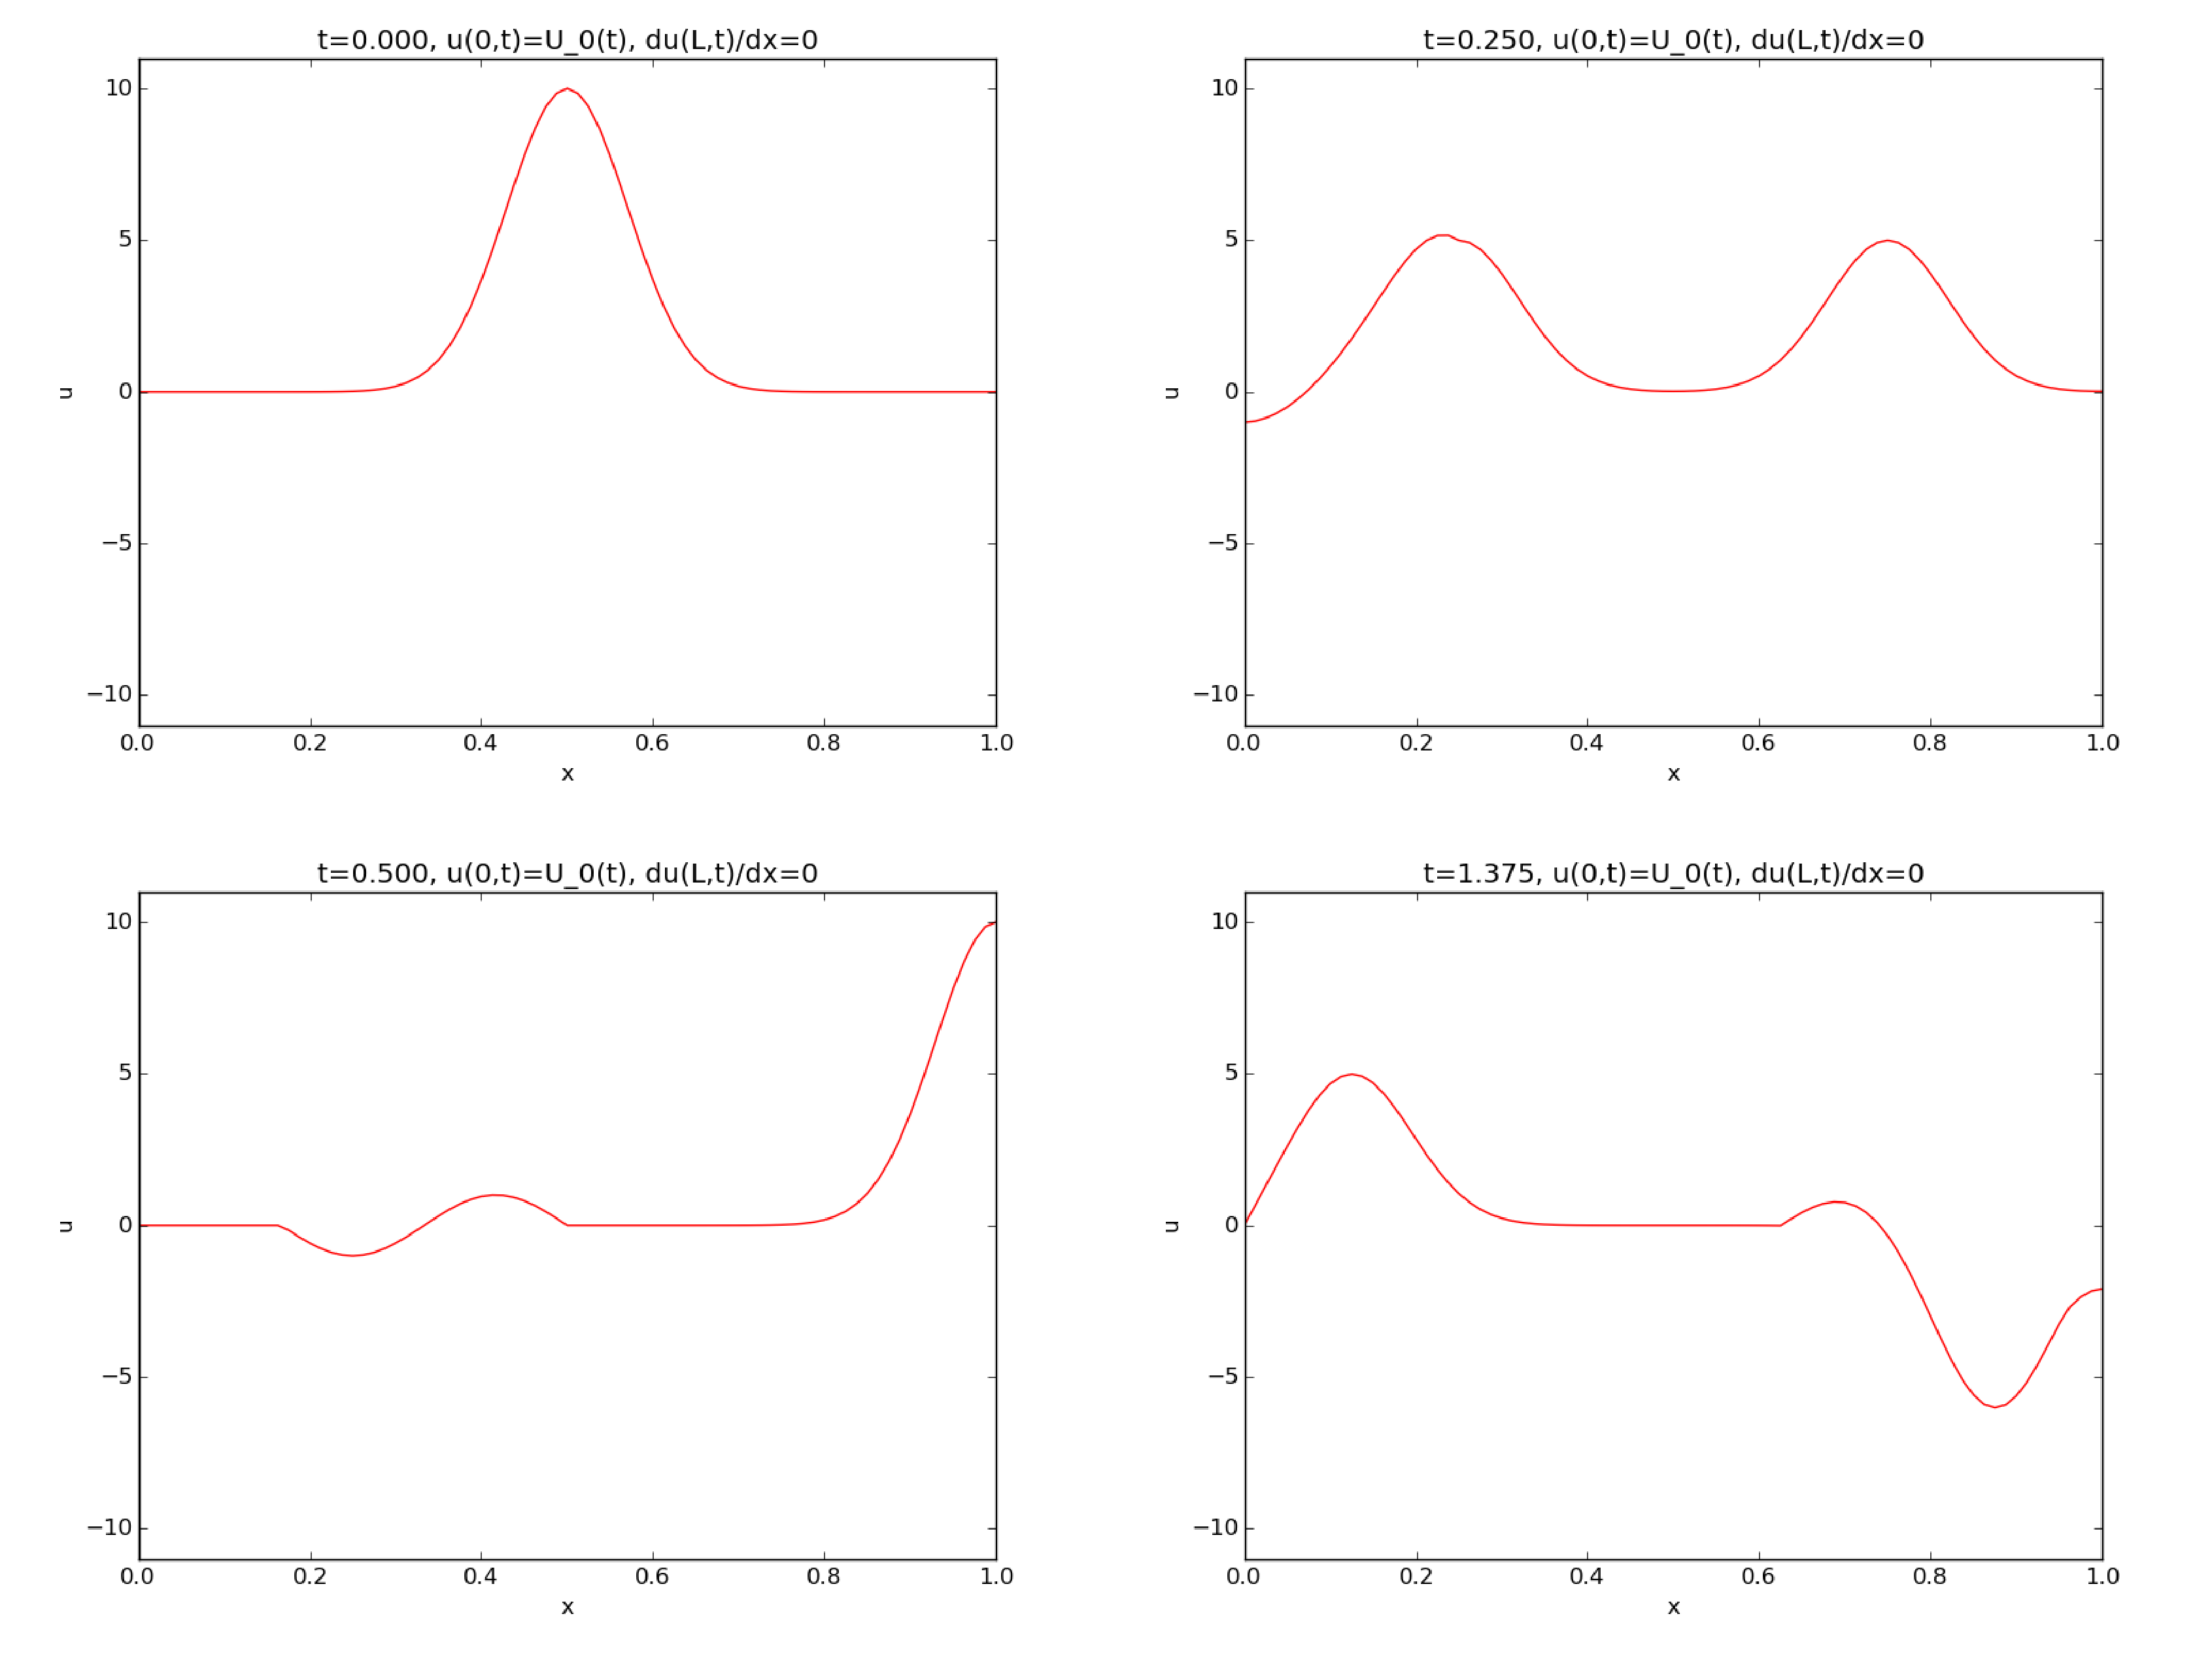
\includegraphics[width=1.0\linewidth]{fig-scaling/gaussian_plus_incoming_alpha10.pdf}}
  \caption{
  Snapshots of solution with large initial condition and small incoming wave ($\alpha=10$). \label{scale:wave:pde2:fig:alpha10}
  }
\end{figure}
%\clearpage % flush figures scale:wave:pde2:fig:alpha10



\begin{figure}[!ht]  % scale:wave:pde2:fig:alpha01
  \centerline{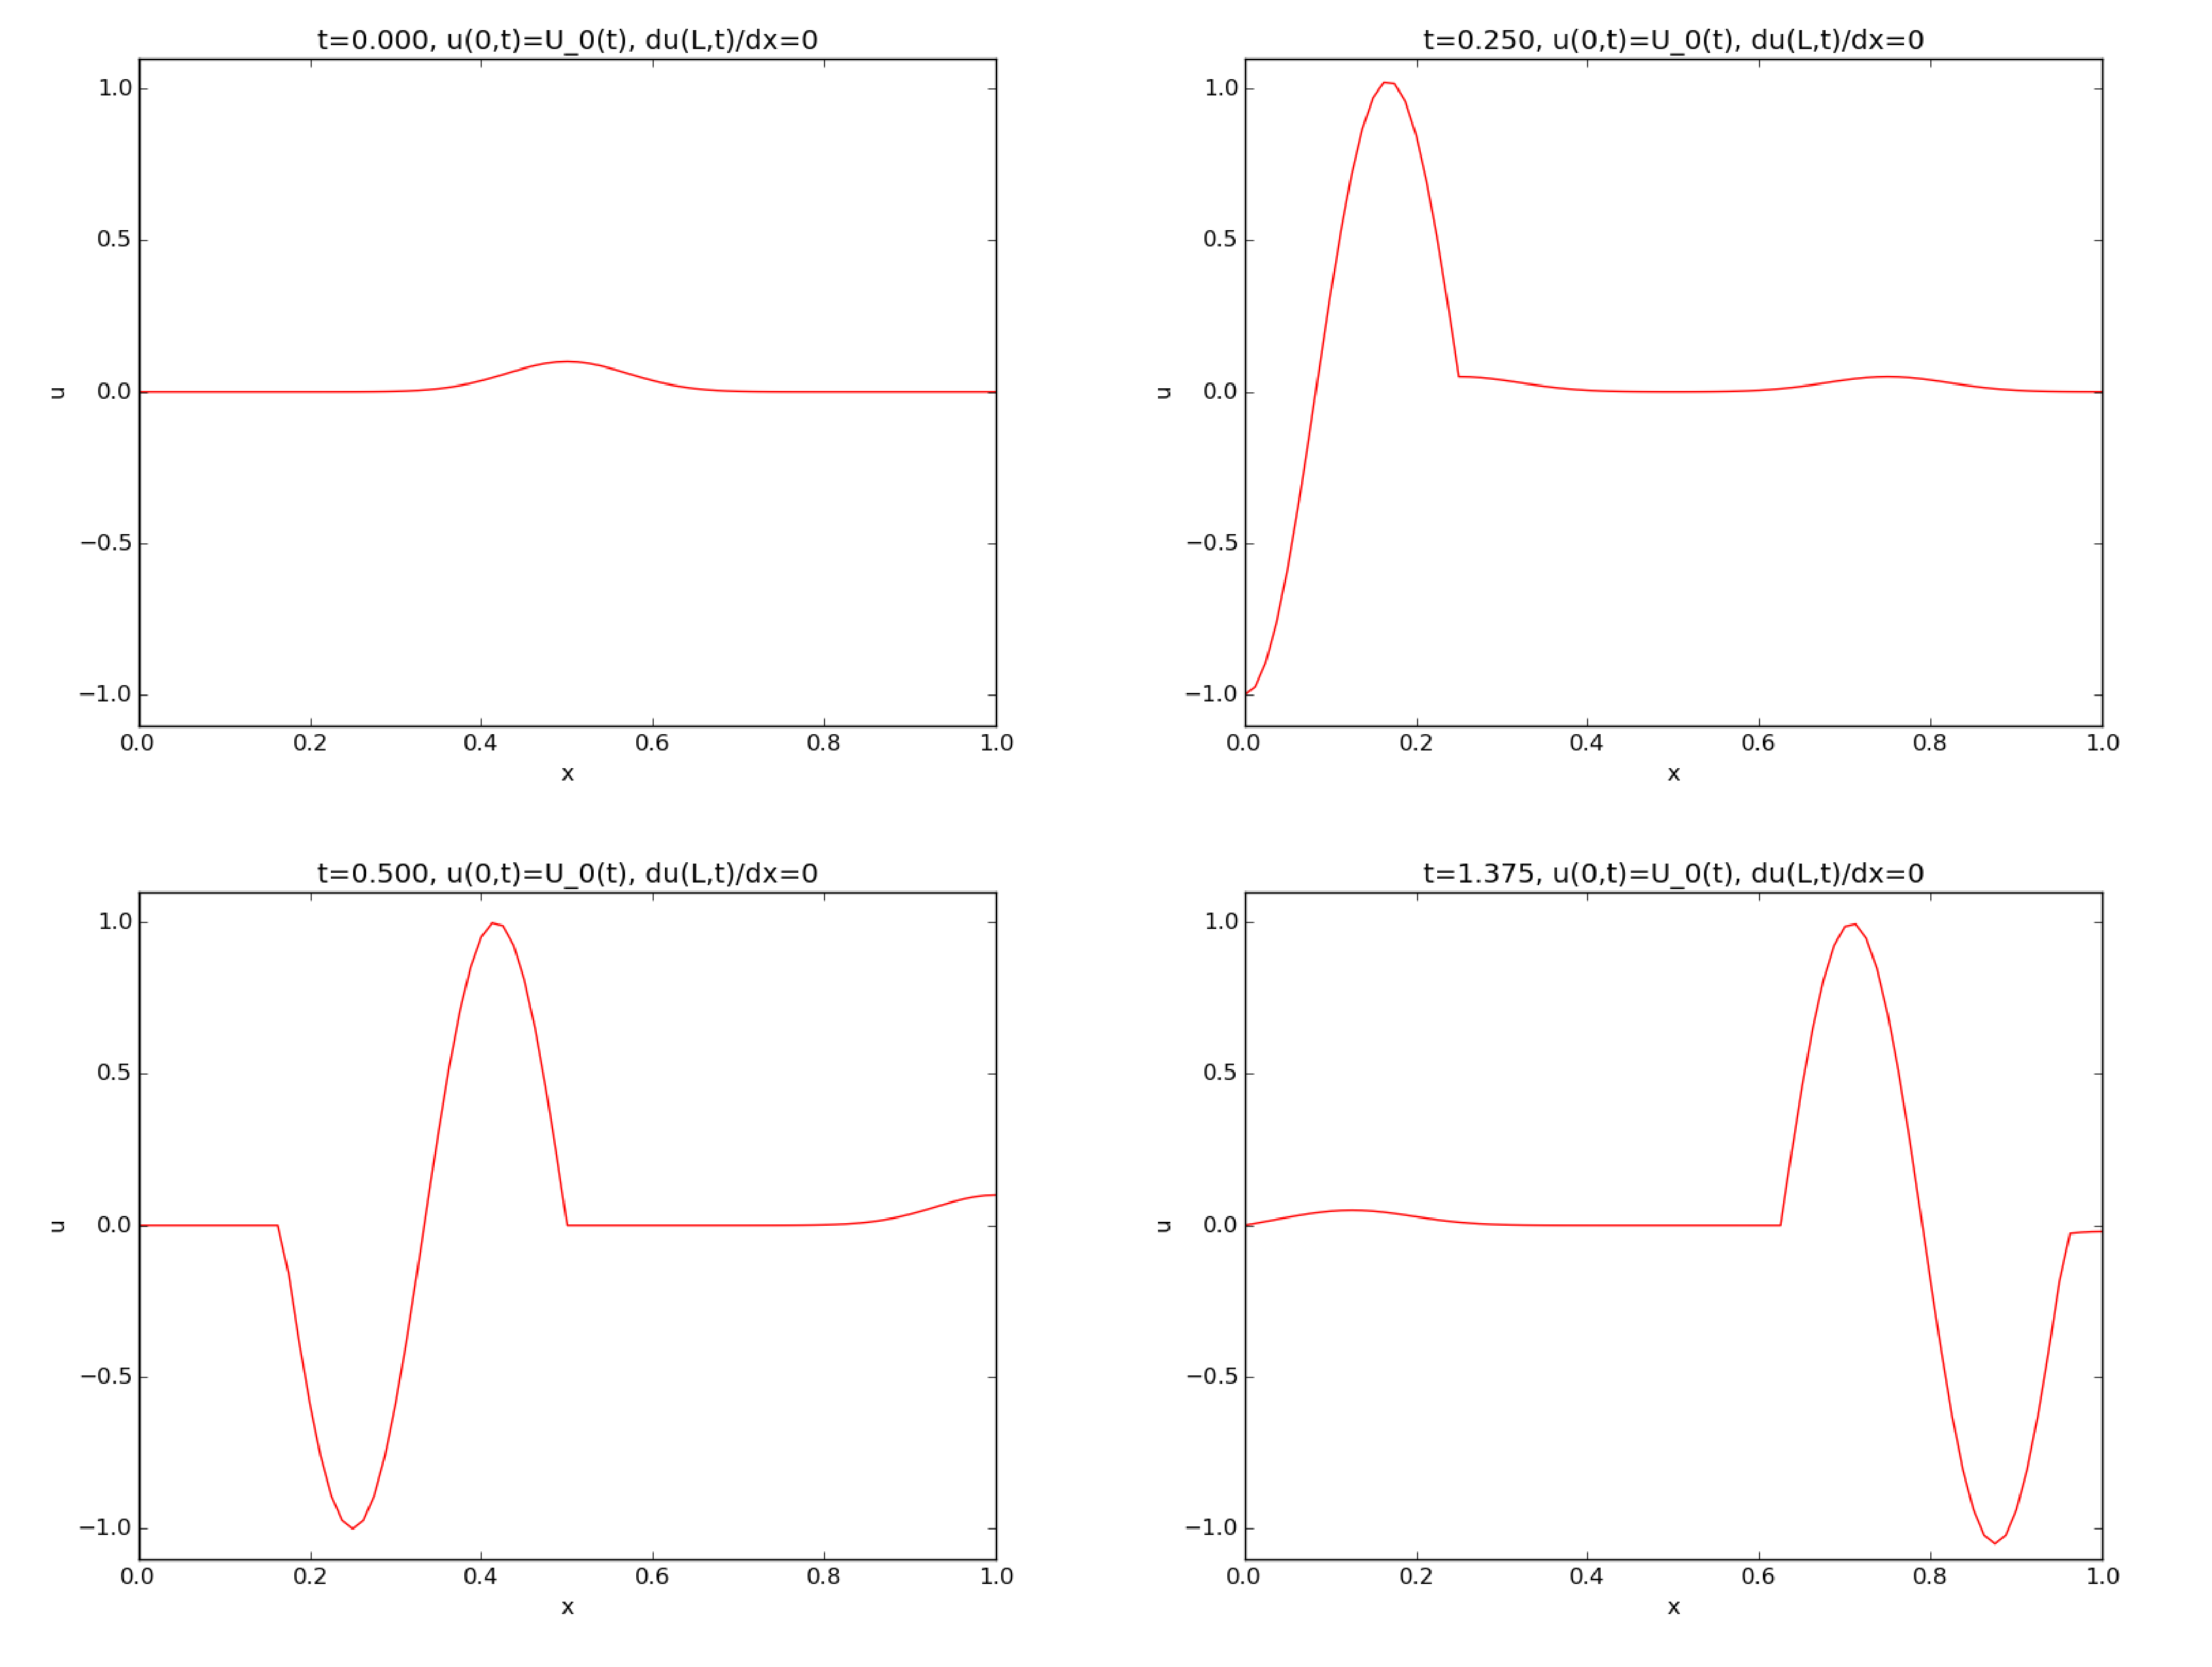
\includegraphics[width=1.0\linewidth]{fig-scaling/gaussian_plus_incoming_alpha01.pdf}}
  \caption{
  Snapshots of solution with small initial condition and large incoming wave ($\alpha=0.1$). \label{scale:wave:pde2:fig:alpha01}
  }
\end{figure}
%\clearpage % flush figures scale:wave:pde2:fig:alpha01



\begin{doconce:movie}
\refstepcounter{doconce:movie:counter}
\begin{quote}
% link to web movie
Movie \arabic{doconce:movie:counter}: $\alpha=10$. \href{https://github.com/hplgit/scaling-book/raw/master/doc/pub/book/html/mov-scaling/gaussian_plus_incoming/alpha10.mp4}{\nolinkurl{https://github.com/hplgit/scaling-book/raw/master/doc/pub/book/html/mov-scaling/gaussian_plus_incoming/alpha10.mp4}}
\end{quote}
\end{doconce:movie}



\begin{doconce:movie}
\refstepcounter{doconce:movie:counter}
\begin{quote}
% link to web movie
Movie \arabic{doconce:movie:counter}: $\alpha=0.1$. \href{https://github.com/hplgit/scaling-book/raw/master/doc/pub/book/html/mov-scaling/gaussian_plus_incoming/alpha01.mp4}{\nolinkurl{https://github.com/hplgit/scaling-book/raw/master/doc/pub/book/html/mov-scaling/gaussian_plus_incoming/alpha01.mp4}}
\end{quote}
\end{doconce:movie}



\subsection{Velocity initial condition}
\label{scale:wave:pde2:Vcond}

Now we change the initial condition from $u=I$ and $\partial u/\partial t = 0$ to

\begin{align}
u(x,0) &= 0,\\ 
\frac{\partial}{\partial t} u(x,0) &= V(x)\tp
\end{align}
Impact problems are often of this kind.
The scaled version of $u_t(x,0)=V(x)$ becomes

\[ \frac{\partial}{\partial \bar t} \bar u(\bar x,0) =
\frac{t_c}{u_c}V(\bar x x_c)\tp
\]

\paragraph{Analytical insight.}
From (\ref{scale:wave:pde:sol:general}) we now get $f_L + f_R =0$ and
$cf_L' - cf_R' = V$. Introducing $W(x)$ such that $W'(x)=V(x)$, a solution
is $f_L=\frac{1}{2}W/c$ and $-f_R=\frac{1}{2}W/c$. We can express this
solution through the formula

\begin{equation}
u(x,t) = \frac{1}{2c}\int_{x-ct}^{x+ct} V(\xi) d\xi
 = \frac{1}{2c}(W(x+ct) - W(x-ct))\tp
 \label{scale:wave:pde2:Vcond:usol}
 \end{equation}

\paragraph{Scaling.}
Since $V$ is the time-derivative of $u$, the characteristic size of
$V$, call it $V_c$, is typically $u_c/t_c$.  If we, as usual, base
$t_c$ on the wave speed, $t_c = L/c$, we get $u_c = V_cL/c$.  Looking
at the solution (\ref{scale:wave:pde2:Vcond:usol}), we see that $u_c$
has size $\hbox{mean}(V)L/(2c)$, where $\hbox{mean}(V)$ is the mean
value of $V$ ($W\sim\hbox{mean}(V)L$). This result suggests
$V_c=\hbox{mean}(V)$ and $u_c = \hbox{mean}(V)L/(2c)$. One may argue
that the factor 2 is not important, but if we want $|\bar u|\in [0,1]$
it is convenient to keep it.

The scaled initial condition becomes

\[ \frac{\partial}{\partial \bar t} \bar u(\bar x,0) =
\frac{t_c}{u_c}V(\bar x x_c) =
\frac{V(\bar x x_c)}{\half\hbox{mean}(V)}\tp
\]


\paragraph{Nonzero initial shape.}
Suppose we change the initial condition $u(x,0)=0$ to $u(x,0)=I(x)$.
The scaled version of this condition with the above $u_c$
based on $V$ becomes

\begin{equation}
\bar u(\bar x, 0) = \frac{2cI(\bar x x_c)}{L\,\hbox{mean}(V)}\tp
\label{scale:wave:pde2:Vcond:eq}
\end{equation}


\begin{notice_mdfboxadmon}[Check that dimensionless numbers are dimensionless!]
Is a dimensionless number really dimensionless?
It is easy to make errors when scaling equations, so checking that
such fractions are dimensionless is wise.
The dimension of $I$ is the same as $u$, here taken to be displacement:
[L].
Since $V$ is $\partial u/\partial t$, its dimension is
$[\hbox{LT}^{-1}]$. The dimensions of $c$ and $L$ are
$[\hbox{LT}^{-1}]$ and $[\hbox{L}]$. The dimension of the right-hand side
of (\ref{scale:wave:pde2:Vcond:eq}) is then

\[ \frac{[\hbox{LT}^{-1}][L]}{[L][L\hbox{T}^{-1}]}
= 1,\]
demonstrating that the fraction is indeed dimensionless.
\end{notice_mdfboxadmon}



One may introduce a dimensionless initial
shape, $\bar I (\bar x)= I(\bar xL)/\max_x |I|$. Then

\[ \bar u(\bar x, 0) = \alpha\bar I(\bar x),\]
where $\alpha$ the dimensionless number

\[ \alpha = \frac{2c}{L}\frac{\max_x |I(x)|}{\hbox{mean}(V)}\tp\]

\index{dimensionless number}

If $V$ is much larger than $I$, one expects that the influence of $I$
is small. However, it takes time for the initial velocity $V$ to
influence the wave motion, so the speed of the waves $c$ and the length
of the domain $L$ also play a role. This is reflected in $\alpha$, which is the
important parameter.
Again, the scaling and the resulting dimensionless parameter(s)
teach us much about the interaction of the various physical effects.

% A large $\alpha$ means that the
% initial wave shape $I$
% travels quickly through the domain before the effect of $V$ becomes
% visible. The impact of $I$ may therefore be significant for small $t$
% (the numerical value of $c/L$ is very large and $\max |I|/\max |V|$ may still
% be somewhat small).
% With $\alpha$ small, not much happens before the effect of $V$ becomes
% visible. Recall that the dimensionless initial velocity is about unity
% regardless of other parameters.
% See exer-scaling/wave1D_small_I_big_V.py for experiments.

\subsection{Variable wave velocity and forcing}
\label{scale:wave:pde2:cvar}

The next generalization regards wave propagation in
a non-homogeneous medium where the wave velocity $c$ depends on the
spatial position: $c=c(x)$. To simplify the notation we introduce
$\lambda (x) = c^2(x)$. We introduce homogeneous Neumann conditions
at $x=0$ and $x=L$. In addition, we add a force term $f(x,t)$
to the PDE, modeling wave generation in the interior of
the domain. For example, a moving slide at the bottom of a fjord
will generate surface waves and is modeled by such an $f(x,t)$ term
(provided the length of the waves is much larger than the depth so
that a simple wave equation like (\ref{scale:wave:pde3}) applies).
The initial-boundary value problem
can be then expressed as

\begin{align}
\frac{\partial^2 u}{\partial t^2} &=
\frac{\partial}{\partial x}\left(
\lambda(x) {\partial u\over\partial x}\right) + f(x,t),
\quad & x\in (0,L),\ t\in (0,T],
\label{scale:wave:pde3}\\ 
u(x,0) &= I(x),
\quad &x\in [0,L],
\label{scale:wave:pde3:ic:u}\\ 
{\partial\over\partial t}u(x,0) &= 0,
\quad & x\in [0,L],
\label{scale:wave:pde3:ic:ut}\\ 
\frac{\partial}{\partial x}u(0,t) & = 0,
\quad  &t\in (0,T],
\label{scale:wave:pde3:bc:0}\\ 
\frac{\partial}{\partial x}u(L,t) & = 0,
\quad  &t\in (0,T].
\label{scale:wave:pde3:bc:L}
\end{align}

\paragraph{Non-dimensionalization.}
We make the coefficient $\lambda$ non-dimensional by

\begin{equation}
\bar\lambda(\bar x) = \frac{\lambda(\bar xx_c)}{\lambda_c},
\end{equation}
where one normally chooses the characteristic size of $\lambda$, $\lambda_c$,
to be the maximum value such that $|\lambda|\leq 1$:

\[ \lambda_c = \max_{x\in(0,L)}\lambda(x)\tp\]
Similarly, $f$ has a scaled version

\[ \bar f(\bar x,\bar t) = \frac{f(\bar x x_c, \bar t t_c)}{f_c},\]
where normally we choose

\[ f_c=\max_{x,t}|f(x,t)|\tp\]
Inserting dependent and independent variables expressed by their
non-dimensional counterparts yields

\begin{align*}
\frac{\partial^2 \bar u}{\partial \bar t^2} &=
\frac{t_c^2\lambda_c}{L^2}\frac{\partial}{\partial \bar x}\left(
\bar\lambda(\bar x) {\partial\bar u\over\partial\bar x}\right)
+ \frac{t_c^2f_c}{u_c}\bar f(\bar x,\bar t),
\quad & \bar x\in (0,1),\ \bar t\in (0,\bar T],\\ 
\bar u(\bar x,0) &= \frac{I(x)}{u_c},
\quad &\bar x\in [0,1],\\ 
{\partial\over\partial \bar t}\bar u(\bar x,0) &= 0,
\quad & \bar x\in [0,1],\\ 
\frac{\partial}{\partial \bar x}\bar u(0,\bar t) & = 0,
\quad  &\bar t\in (0,\bar T],\\ 
\frac{\partial}{\partial \bar x}\bar u(1,\bar t) & = 0,
\quad  &\bar t\in (0,\bar T],
\end{align*}
with $\bar T = Tc/L$.


\paragraph{Choosing the time scale.}
The time scale is, as before, chosen as $t_c
=L/\sqrt{\lambda_c}$. Note that the previous (constant) wave velocity
$c$ now corresponds to $\sqrt{\lambda (x)}$.  Therefore,
$\sqrt{\lambda_c}$ is a characteristic wave velocity.

One could wonder if the time scale of the force term, $f(x,t)$,
should influence $t_c$, but as we reasoned for the boundary condition
$u(0,t)=U_L(t)$, we let the characteristic time be governed by the
signal speed in the medium, i.e., by $\sqrt{\lambda_c}$ here and not
by the time scale of the excitation $f$, which dictates the
length of the generated waves and not their propagation speed.

\paragraph{Choosing the spatial scale.}
We may choose $u_c$ as $\max_x |I(x)|$, as before,
or we may fit $u_c$ such that the coefficient in the source term
is unity, i.e., all terms balance each other.
This latter idea leads to

\[ u_c = \frac{L^2 f_c}{\lambda_c} \]
and a PDE without parameters,

\[
\frac{\partial^2 \bar u}{\partial \bar t^2} =
\frac{\partial}{\partial \bar x}\left(
\bar\lambda(\bar x) {\partial\bar u\over\partial\bar x}\right)
+ \bar f(\bar x,\bar t)\tp
\]
The initial condition $u(x,0)=I(x)$ becomes in dimensionless form

\[ \bar u(\bar x, 0) = u_c^{-1} \max_x |I(x)|\bar I(\bar x) =
\beta^{-1}\bar I(\bar x),\]
where

\[ \beta = \frac{L^2}{\lambda_c}\frac{\max_{x,t} |f(x,t)|}{\max_x|I(x)|}\tp\]

In the case $u_c=\max_x|I(x)|$, $\bar u(\bar x,0)=\bar I(\bar x)$ and
the $\beta$ parameter appears in the PDE instead:

\[
\frac{\partial^2 \bar u}{\partial \bar t^2} =
\frac{\partial}{\partial \bar x}\left(
\bar\lambda(\bar x) {\partial\bar u\over\partial\bar x}\right)
+ \beta \bar f(\bar x,\bar t)\tp
\]
With $V=0$, and $u=0$ or $u_x=0$ on the boundaries $x=0,L$, this scaling normally gives
$|\bar u|\leq 1$, since initially $|I|\leq 1$, and no boundary condition
can increase the amplitude.
However, the forcing, $\bar f$, may inherit spatial and temporal scales of its
own that may complicate the matter. The forcing may, for instance, be
some disturbance moving with a velocity close to the propagation velocity of
the free waves. This will have an effect akin to the resonance for the vibration problem discussed in
section~\ref{sec:scale:vib:undamped:mg} and the waves produced by the forcing may be much larger than
indicated by $\beta$. On the other hand, the forcing may also consist
of alternating positive and negative parts (retrogressive slides constitute an
example). These may interfere to
reduce the wave generation by an order of magnitude.

\paragraph{Scaling the velocity initial condition.}
The initial condition $u_t(x,0)=V(x)$ has its dimensionless variant as

\[ \bar V(\bar x) = \frac{t_c}{u_c}\frac{V(L\bar x)}{\max_x|V(x)|},\]
which becomes

\[ \frac{\partial\bar u}{\partial\bar t}(\bar x, 0) =
\frac{L}{\sqrt{\lambda_c}}\frac{\max_{x}|V(x)|}{\max_{x}|I(x)|}\bar V(\bar x),
\hbox{ if } u_c=\max_x|I(x)|,\]
or

\[ \frac{\partial\bar u}{\partial\bar t}(\bar x, 0) =
\frac{\sqrt{\lambda_c}}{L}\frac{\max_{x}|V(x)|}{\max_{x,t}|f(x,t)|}
\bar V(\bar x),
\hbox{ if } u_c=t_c^2f_c=\frac{L^2}{\lambda_c}\max_{x,t}|f(x,t)|\tp\]
Introducing the dimensionless number $\alpha$ (cf.~Section~\ref{scale:wave:pde2:Vcond}),

\[ \alpha^{-1} = \frac{\sqrt{\lambda_c}}{L}\frac{\max_{x}|V(x)|}{\max_{x,t}|f(x,t)|},
\]
we can write

\[
\frac{\partial\bar u}{\partial\bar t}(\bar x, 0) =
\left\lbrace \begin{array}{ll}
\alpha^{-1}\bar V(\bar x),& u_c=\max_x|I|\\ 
\alpha^{-1}\beta^{-1}\bar V(\bar x), & u_c=t_c^2f_c
\end{array}\right.
\]

\subsection{Damped wave equation}
\label{scale:wave:pde2:damped}

A linear damping term $b\,\partial u/\partial t$ is often added to
the wave equation to model energy dissipation and amplitude reduction.
Our PDE then reads

\begin{equation}
\frac{\partial^2 u}{\partial t^2}
+ b\frac{\partial u}{\partial t} =
\frac{\partial}{\partial x}\left(
\lambda(x) {\partial u\over\partial x}\right) + f(x,t)\tp
\end{equation}
The scaled equation becomes

\[
\frac{\partial^2 \bar u}{\partial \bar t^2}
+ \frac{t_c} b\frac{\partial \bar u}{\partial \bar t} =
\frac{t_c^2\lambda_c}{L^2}\frac{\partial}{\partial \bar x}\left(
\bar \lambda(\bar x) {\partial \bar u\over\partial \bar x}\right) +
\frac{t_c^2f_c}{u_c}\bar f(\bar x,\bar t)\tp
\]

The damping term is usually much smaller than the two other terms involving
$\bar u$. The time scale is therefore chosen as in the undamped case,
$t_c=L/\sqrt{\lambda_c}$. As in Section~\ref{scale:wave:pde2:cvar},
we have two choices of $u_c$: $u_c=\max_x|I|$ or $u_c=t_c^2f_c$.
The former choice of $u_c$ gives a PDE with two dimensionless numbers,

\begin{equation}
\frac{\partial^2 \bar u}{\partial \bar t^2}
+ \gamma\frac{\partial \bar u}{\partial \bar t} =
\frac{\partial}{\partial \bar x}\left(
\bar \lambda(\bar x) {\partial\bar u\over\partial\bar x}\right) +
\beta\bar f(\bar x,\bar t),
\end{equation}
where

\[ \gamma = \frac{bL}{\sqrt{\lambda_c}}, \]
measures the size of the damping, and $\beta$ is as given
in Section~\ref{scale:wave:pde2:cvar}.
With $u_c=t_c^2f_c$ we get a PDE where only $\gamma$ enters,

\begin{equation}
\frac{\partial^2 \bar u}{\partial \bar t^2}
+ \gamma\frac{\partial \bar u}{\partial \bar t} =
\frac{\partial}{\partial \bar x}\left(
\bar \lambda(\bar x) {\partial\bar u\over\partial\bar x}\right) +
\bar f(\bar x,\bar t)\tp
\end{equation}
The scaled initial conditions are as in
Section~\ref{scale:wave:pde2:cvar}, so in this latter case
$\beta$ appears in the initial condition for $u$.

To summarize, the effects of $V$, $f$, and damping are reflected in
the dimensionless numbers $\alpha$, $\beta$, and $\gamma$,
respectively.

\subsection{A three-dimensional wave equation problem}

To demonstrate how the scaling extends to in three spatial dimensions,
we consider

\begin{equation}
\frac{\partial^2 \bar u}{\partial \bar t^2} =
\frac{\partial}{\partial x}\left(\lambda\frac{\partial u}{\partial x}\right)+
\frac{\partial}{\partial y}\left(\lambda\frac{\partial u}{\partial y}\right)+
\frac{\partial}{\partial z}\left(\lambda\frac{\partial u}{\partial z}\right)\tp
\end{equation}
Introducing

\[ \bar x = \frac{x}{x_c},\quad \bar y = \frac{y}{y_c},
   \quad \bar z = \frac{z}{z_c},
   \quad \bar t = \frac{t}{t_c}, \quad \bar u =\frac{u}{u_c},\]
and scaling $\lambda$ as
$\bar\lambda = \lambda(\bar xx_c, \bar y y_c, \bar z z_c)/\lambda_c$,
we get

\[
\frac{\partial^2 \bar u}{\partial \bar t^2} =
\frac{t_c^2\lambda_c}{x_c^2}\frac{\partial}{\partial \bar x}\left(\bar\lambda\frac{\partial \bar u}{\partial \bar x}\right)+
\frac{t_c^2\lambda_c}{y_c^2}\frac{\partial}{\partial \bar y}\left(\bar\lambda\frac{\partial \bar u}{\partial \bar y}\right)+
\frac{t_c^2\lambda_c}{z_c^2}\frac{\partial}{\partial \bar z}\left(\bar\lambda\frac{\partial \bar u}{\partial \bar z}\right)\tp
\]
Often, we will set $x_c=y_c=z_c=L$ where $L$ is some characteristic
size of the domain.
As before, $t_c = L/\sqrt{\lambda_c}$, and these choices lead to a
dimensionless wave equation without physical parameters:

\begin{equation}
\frac{\partial^2 \bar u}{\partial \bar t^2} =
\frac{\partial}{\partial \bar x}\left(\bar\lambda\frac{\partial \bar u}{\partial \bar x}\right)+
\frac{\partial}{\partial \bar y}\left(\bar\lambda\frac{\partial \bar u}{\partial \bar y}\right)+
\frac{\partial}{\partial \bar z}\left(\bar\lambda\frac{\partial \bar u}{\partial \bar z}\right)\tp
\end{equation}
The initial conditions remain the same as in the previous one-dimensional
examples.

% !split
\section{The diffusion equation}
\label{sec:scale:diffu}

The diffusion equation in a one-dimensional homogeneous medium reads

\begin{equation}
\frac{\partial u}{\partial t} =
\dfc\frac{\partial^2 u}{\partial x^2}, \quad  x\in (0,L),\ t\in (0,T],
\label{sec:scale:diffu:pde1}
\end{equation}
where $\dfc$ is the diffusion coefficient. The
multi-dimensional generalization to a heterogeneous medium
and a source term takes the form

\begin{equation}
\frac{\partial u}{\partial t} =
\nabla\cdot\left(\dfc \nabla u\right) + f, \quad  x,y,z\in \Omega,\ t\in (0,T]\tp
\label{sec:scale:diffu:pde1:3D}
\end{equation}
We first look at scaling of the PDE itself, and thereafter we discuss
some types of boundary conditions and how to scale the complete
initial-boundary value problem.


\subsection{Homogeneous 1D diffusion equation}
\label{sec:scale:diffu:homo1D}

\paragraph{Choosing the time scale.}
To make (\ref{sec:scale:diffu:pde1}) dimensionless,
we introduce, as usual, dimensionless dependent and independent variables:

\[ \bar x = \frac{x}{x_c},
\quad \bar t = \frac{t}{t_c}, \quad \bar u =\frac{u}{u_c}\tp\]
Inserting the dimensionless quantities in the one-dimensional
PDE (\ref{sec:scale:diffu:pde1}) results in

\[
\frac{\partial \bar u}{\partial \bar t} =
\frac{t_c\dfc}{L^2}
\frac{\partial^2 \bar u}{\partial \bar x^2}, \quad  \bar x\in (0,1),\ \bar t\in (0,\bar T = T/t_c]\tp
\label{sec:scale:diffu:pde1:d0}
\]
Arguing, as for the wave equation, that the scaling should result in

\[ \frac{\partial \bar u}{\partial \bar t}\hbox{ and }
\frac{\partial^2 \bar u}{\partial \bar x^2}\]
of the same size (about unity),
implies $t_c\dfc/L^2=1$ and therefore $t_c = L^2/\dfc$.

\paragraph{Analytical insight.}
The best way to obtain the scales inherent in a problem is to obtain
an exact analytic solution, as we have done in many of the ODE
examples in this booklet. However, as a rule this is not possible.
Still, often highly
simplified analytic solutions can be found for parts of the problem,
or for some closely related problem. Such solutions may provide
crucial guidance to the nature of the complete solution and to the
appropriate scaling of the full problem. We will employ such solutions
now to learn about scales in diffusion problems.

One can show that $u=Ae^{-pt}\sin (kx)$ is a solution of
(\ref{sec:scale:diffu:pde1}) if $p=\dfc k^2$, for any $k$.
This is the typical solution arising from separation of variables
and reflects the dynamics of the space and time in the PDE.
Exponential decay in
time is a characteristic feature of diffusion processes, and
the e-folding time can then be taken as a time scale. This means
$t_c = 1/p \sim k^{-2}$. Since $k$ is related to the spatial
wave length $\lambda$
through $k=2\pi/\lambda$, it means that $t_c$ depends strongly on the wave
length of the sine term $\sin(kx)$.
In particular, short waves (as found in noisy signals) with
large $k$ decay very rapidly.
For the overall solution we are interested in how the longest meaningful
wave decays and use that time scale for $t_c$. The longest wave
typically has half a wave length over the domain $[0,L]$:
$u = Ae^{-pt}\sin(\pi x/L)$ ($k=\pi/L$), provided $u(0,t)=u(L,t)=0$
(with $u_x(L,t)=0$, the longest wave is $L/4$, but we look at the
case with the wave length $L/2$). Then $t_c=L^2/\dfc \pi^{-2}$,
but the factor $\pi^{-2}$ is not important and we simply choose
$t_c=L^2/\dfc$, which equals the time scale we arrived at above.
We may say that $t_c$ is the time it takes for the diffusion to
significantly change the solution in the entire domain.

Another fundamental solution of the diffusion equation is the
diffusion of a Gaussian function: $u(x,t)=K(4\pi\dfc
t)^{-1/2}\exp{(-x^2/(4\dfc t))}$, for some constant $K$ with
the same dimension as $u$. For the diffusion to be significant
at a distance $x=L$, we may demand the exponential factor to have a
value of $e^{-1}\approx 0.37$, which implies $t=L^2/(4\dfc)$, but the
factor 4 is not of importance, so again, a relevant time scale is
$t_c=L^2/\dfc$.

\paragraph{Choosing other scales.}
The scale $u_c$ is chosen according to the initial condition:
$u_c=\max_{x\in(0,L)}|I(x)|$. For a diffusion equation $u_t=\dfc u_{xx}$
with $u=0$ at the boundaries $x=0,L$, the solution is bounded by
the initial condition $I(x)$. Therefore, the listed choice of $u_c$
implies that
$|u|\leq 1$. (The solution $u=Ae^{-pt}\sin (kx)$ is such an example
if $k=n\pi/L$ for integer $n$ such that $u=0$ for $x=0$ and $x=L$.)

The resulting dimensionless PDE becomes

\begin{equation}
\frac{\partial \bar u}{\partial \bar t} =
\frac{\partial^2 \bar u}{\partial \bar x^2}, \quad  \bar x\in (0,1),\ \bar t\in (0,\bar T],
\label{sec:scale:diffu:pde1:d}
\end{equation}
with initial condition

\[ \bar u(\bar x, 0) = \bar I(\bar x) = \frac{I(x_c\bar x)}{\max_x |I(x)|}\tp\]
Notice that (\ref{sec:scale:diffu:pde1:d}) is without physical parameters,
but there may be parameters in $I(x)$.

\subsection{Generalized diffusion PDE}

Turning the attention to (\ref{sec:scale:diffu:pde1:3D}), we introduce
the dimensionless diffusion coefficient

\[ \bar\dfc(\bar x,\bar y,\bar z) =
\dfc_c^{-1}\dfc (x_c\bar x, y_c\bar y, z_c\bar z),\]
typically with

\[ \dfc_c = \max_{x,y,z}\dfc(x,y,z)\tp\]
The length scales are

\[ \bar x = \frac{x}{x_c},\quad \bar y = \frac{y}{y_c},\quad
\bar z = \frac{z}{z_c}\tp
\]
We scale $f$ in a similar fashion:

\[ \bar f(\bar x, \bar y, \bar z, \bar t)
= f_c^{-1}f(\bar xx_c, \bar yy_c \bar zz_c, \bar tt_c),\]
with

\[ f_c = \max_{x,y,z,t}|f(x,y,z,t)|\tp\]
Also assuming
that $x_c=y_c=z_c=L$, and $u_c=\max_{x,y,z}(I(x,y,z)$,
we end up with the scaled PDE

\begin{equation}
\frac{\partial \bar u}{\partial \bar t} =
\nabla\cdot\left(\bar\dfc \bar\nabla \bar u\right) + \beta\bar f, \quad  \bar x,\bar y,\bar z\in \bar \Omega,\ \bar t\in (0,\bar T]\tp
\label{sec:scale:diffu:pde1:3D:d}
\end{equation}
Here, $\bar\nabla$ means differentiation with respect to dimensionless
coordinates $\bar x$, $\bar y$, and $\bar z$. The dimensionless parameter
$\beta$ takes the form

\[ \beta = \frac{t_cf_c}{u_c} = \frac{L^2}{\dfc}
\frac{\max_{x,y,z,t}|f(x,y,z,t)|}{\max_{x,y,z}|I(x,y,z)|}\tp\]
The scaled initial condition is $\bar u = \bar I$ as in the 1D case.

An alternative choice of $u_c$ is to make the coefficient $t_cf_c/u_c$
in the source term unity. The scaled PDE now becomes

\begin{equation}
\frac{\partial \bar u}{\partial \bar t} =
\bar\nabla\cdot\left(\bar\dfc \bar\nabla \bar u\right) + f,
\label{sec:scale:diffu:pde1:3D:d2}
\end{equation}
but the initial condition features the $\beta$ parameter:

\[ \bar u(\bar x, \bar y, \bar z, 0) = \frac{I}{t_cf_c} =
\beta^{-1}\bar I(\bar x,\bar y,\bar z)\tp
\]

The $\beta$ parameter can be interpreted as the ratio of the source
term and the terms with $u$:

\[ \beta = \frac{f_c}{u_c/t_c}\sim \frac{|f|}{|u_t|},\quad
\beta = \frac{f_c}{u_c/t_c} = \frac{f_c}{L^2/t_c u_c/L^2}\sim
\frac{|f_c|}{|\dfc\nabla^2 u|}\tp
\]

We may check that $\beta$ is really non-dimensional. From the PDE,
$f$ must have the same dimensions as $\partial u/\partial t$, i.e.,
$[\Theta\hbox{T}^{-1}]$.
The dimension of $\dfc$ is more intricate, but from the term
$\dfc u_{xx}$ we know that $u_{xx}$ has dimensions $[\Theta\hbox{L}^{-2}]$,
and then $\dfc$ must have dimension $[\hbox{L}^2\hbox{T}^{-1}]$
to match the target $[\Theta\hbox{T}^{-1}]$.
In the expression for $\beta$ we get
$[\hbox{L}^2\Theta\hbox{T}^{-1}(\hbox{L}^2\hbox{T}^{-1}\Theta)^{-1}]$,
which equals 1 as it should.


\subsection{Jump boundary condition}

A classical one-dimensional heat conduction problem goes as
follows. An insulated rod at some constant temperature $U_0$ is
suddenly heated from one end ($x=0$), modeled as a constant Dirichlet
condition $u(0,t)=U_1\neq U_0$ at that end. That is, the boundary
temperature jumps from $U_0$ to $U_1$ at $t=0$. All the other surfaces
of the rod are insulated such that a one-dimensional model is
appropriate, but we must explicitly demand $u_x(L,t)=0$ to incorporate
the insulation condition in the one-dimensional model at the end
of the domain $x=L$.  Heat cannot
escape, and since we supply heat at $x=0$, all of the material will
eventually be warmed up to the temperature $U_1$: $u\rightarrow U_1$
as $t\rightarrow\infty$.

The initial-boundary value problem reads

\begin{align}
\varrho c \frac{\partial u}{\partial t} &=
k \frac{\partial^2 u}{\partial x^2},
\quad &  x\in (0,L),\ t\in (0, T],
\label{scale:heat:pde3}\\ 
u(x,0) &= U_0,
\quad & x\in [0,L],
\label{scale:heat:pde3:ic:u}\\ 
u(0, t) & = U_1,
\quad  & t\in (0, T],
\label{scale:heat:pde3:bc:0}\\ 
\frac{\partial}{\partial x} u(L, t) & = 0,
\quad & t\in (0, T].
\label{scale:heat:pde3:bc:L}
\end{align}
The PDE (\ref{scale:heat:pde3}) arises from the energy equation in
solids and involves three physical parameters: the density $\varrho$,
the specific heat capacity parameter $c$,a nd the heat conduction
coefficient (from Fourier's law). Dividing by $\varrho c$ and
introducing $\dfc = k/(\varrho c)$ brings (\ref{scale:heat:pde3}) on
the standard form (\ref{sec:scale:diffu:pde1}). We just use the
$\dfc$ parameter in the following.

The natural dimensionless temperature for this problem is

\[ \bar u = \frac{u - U_0}{U_1 - U_0},\]
since this choice makes $\bar u\in [0,1]$. The reason is that $u$ is bounded by
the initial and boundary conditions (in the absence of a source term in
the PDE),
and we have
$\bar u(\bar x,0)=0$, $\bar u(\bar x,\infty)=1$, and $
\bar u(0,\bar t)=1$.

The choice of $t_c$ is as in the previous cases. We arrive at
the dimensionless initial-boundary value problem

\begin{align}
\frac{\partial \bar u}{\partial \bar t} &=
\frac{\partial^2 \bar u}{\partial \bar x^2},
\quad &  \bar x\in (0,1),\ \bar t\in (0, \bar T],
\label{scale:heat:pde3:d}\\ 
\bar u(\bar x,0) &= 0,
\quad & \bar x\in [0,1],
\label{scale:heat:pde3:ic:u:d}\\ 
\bar u(0, \bar t) & = 1,
\quad  & \bar t\in (0, \bar T],
\label{scale:heat:pde3:bc:0:d}\\ 
\frac{\partial}{\partial \bar x} u(1, \bar t) & = 0,
\quad & \bar t\in (0, \bar T].
\label{scale:heat:pde3:bc:L:d}
\end{align}
The striking feature is that there are no physical parameters left in
this problem. One simulation can be carried out for $\bar u(\bar x,\bar t)$,
see Figure~\ref{scale:heat:pde3:fig},
and the temperature in a rod of any material and any constant initial and
boundary temperature can be retrieved by

\[ u(x,t) = U_0 + (U_1-U_0)\bar u(x/L, t\dfc/L^2)\tp\]


\begin{figure}[!ht]  % scale:heat:pde3:fig
  \centerline{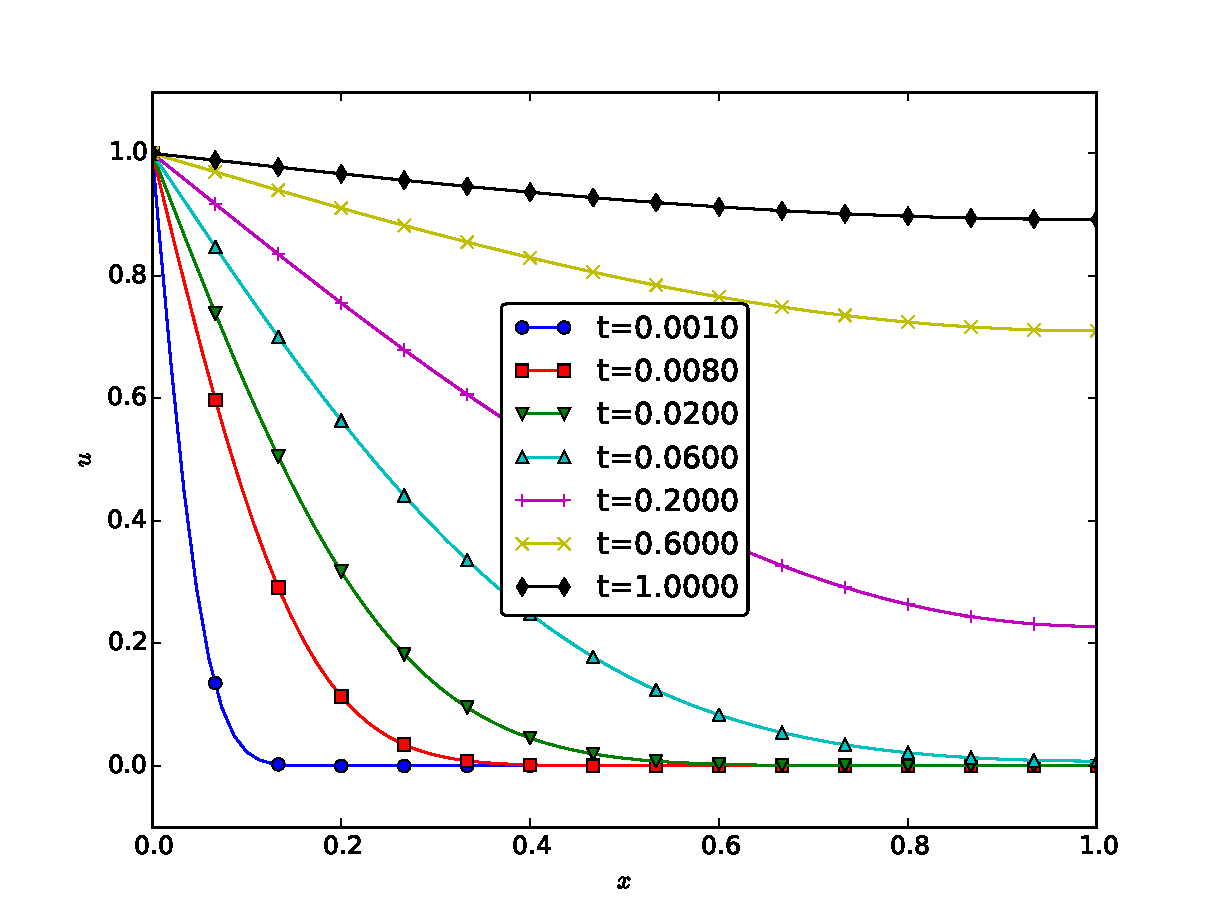
\includegraphics[width=0.8\linewidth]{fig-scaling/diffusion_jump_BC.pdf}}
  \caption{
  Scaled temperature in an isolated rod suddenly heated from the end. \label{scale:heat:pde3:fig}
  }
\end{figure}
%\clearpage % flush figures scale:heat:pde3:fig



\subsection{Oscillating Dirichlet condition}

Now we address a heat equation problem where the temperature is
oscillating on the boundary $x=0$:

\begin{align}
\frac{\partial u}{\partial t} &=
\dfc \frac{\partial^2 u}{\partial x^2},
\quad &  x\in (0,L),\ t\in (0, T],
\label{scale:heat:pde2}\\ 
u(x,0) &= U_0,
\quad & x\in [0,L],
\label{scale:heat:pde2:ic:u}\\ 
u(0, t) & = U_0 + A\sin(\omega t),
\quad  & t\in (0, T],
\label{scale:heat:pde2:bc:0}\\ 
\frac{\partial}{\partial x} u(L, t) & = 0,
\quad & t\in (0, T].
\label{scale:heat:pde2:bc:L}
\end{align}
One important physical application is temperature oscillations in the
ground, either day and night variations
at a short temporal and spatial scale, or seasonal variations in the
Earth's crust.
An important modeling assumption is (\ref{scale:heat:pde2:bc:L}),
which means that the boundary $x=L$ is placed sufficiently far from $x=0$
such that the solution is much damped and basically constant so
$u_x=0$ is a reasonable condition.

\paragraph{Scaling issues.}
Since the boundary temperature is oscillating around the initial
condition, we expect $u\in [U_0-A,U_0+A]$.
The dimensionless temperature is therefore taken as

\[ \bar u = \frac{u-U_0}{2A},\]
such that $\bar u\in [-1,1]$.

What is an appropriate time scale? There will be two time scales involved,
the oscillations $\sin(\omega t)$ with period $P=2\pi/\omega$ at
the boundary and the ``speed of diffusion'', or more specifically
the ``speed of heat conduction'' in the present context,
where $t_c=x_c^2/\dfc$ is the appropriate scale, $x_c$ being
the length scale. Choosing the right length scale is not obvious. As
we shall see, the standard choice $x_c=L$ is not a good candidate, but
to understand why, we need to examine the solution, either through
simulations or through a closed-form formula. We are so lucky in this
relatively simple pedagogical problem that one can find an exact solution
of a related problem.

\paragraph{Exact solution.}
As usual, investigating the exact solution of the model problem can
illuminate the involved scales. For this particular initial-boundary
value problem the exact solution as $t\rightarrow\infty$
(such that
the initial condition $u(x,0)=U_0$ is forgotten)
and $L\rightarrow\infty$ (such that (\ref{scale:heat:pde2:bc:L})
is certainly valid) can be shown to be

\begin{equation}
u(x,t) = U_0 - Ae^{-bx}\sin (bx - \omega t),\quad b =\sqrt{\frac{\omega}{2\dfc}}\tp
\label{scale:heat:daynight:sol}
\end{equation}
This solution is of the form $e^{-bx}g(x-ct)$, i.e., a damped wave that
moves to the right with velocity $c$ and a damped amplitude $e^{-bx}$.
This is perhaps more easily seen if we make a rewrite

\[ u(x,t) = U_0 - Ae^{-bx}\sin\left(b(x - ct)\right),\quad
c=\omega/b = \sqrt{2\dfc\omega},\  b =\sqrt{\frac{\omega}{2\dfc}}\tp\]

\paragraph{Time and length scales.}
The boundary oscillations lead to the time scale $t_c=1/\omega$.
The speed of the wave suggests another time scale: the time it
takes to propagate through the domain, which is $L/c$, and
hence $t_c = L/c = L/\sqrt{2\dfc\omega}$.

One can argue that $L$ is not the appropriate length scale, because
$u$ is damped by $e^{-bx}$. So, for $x > 4/b$, $u$ is close to zero.
We may instead use $1/b$ as length scale, which is the e-folding distance of the
damping factor, and base
$t_c$ on the time it takes a signal to propagate one length scale,
$t_c^{-1}=bc=\omega$. Similarly, the time scale based on
the ``speed of diffusion'' changes to
$t_c^{-1}= b^2\dfc = \half\omega$ if we employ $1/b$ as length scale.

To summarize, we have three candidates for the time scale:
$t_c=L^2/\dfc$ (diffusion through the entire domain), $t_c=2/\omega$
(diffusion through a distance $1/b$ where $u$ is significantly
different from zero), and $t_c=1/\omega$ (wave movement over a
distance $1/b$).

Let us look at the dimensionless exact solution to see if it can help
with the choice of scales.  We introduce the dimensionless parameters

\[ \beta = bx_c = x_c\sqrt{\frac{\omega}{2\dfc}},\quad
\gamma = \omega t_c\tp\]
The scaled solution becomes

\[ \bar u(\bar x, \bar t; \beta,\gamma) = e^{-\beta\bar x}\sin(\gamma\bar t- \beta\bar x)\tp\]
The three choices of $\gamma$, implied by the three choices of $t_c$, are

\begin{equation}
\gamma = \left\lbrace\begin{array}{ll}
1, & t_c=1/\omega,\\ 
2, & t_c = 2/\omega,\\ 
2\beta^2, & t_c = L^2/\dfc,\ x_c=L
\end{array}\right.
\label{scale:heat:daynight:gamma3}
\end{equation}
The former two choices leave only $\beta$ as parameter in $\bar u$,
and with $x_c=1/b$ as length scale, $\beta$ becomes unity, and there
are no parameters in the dimensionless solution:

\begin{equation}
\bar u(\bar x, \bar t) = e^{-\bar x}\sin(\bar t - \bar x)\tp
\label{scale:heat:daynight:xcb}
\end{equation}
Therefore, $x_c=1/b$ and $t_c=1/\omega$ (or $t_c=2/\omega$, but the
factor 2 is of no importance) are the most appropriate scales.

To further argue why (\ref{scale:heat:daynight:xcb}) demonstrates
that these scales are
preferred, think of
$\omega$ as large. Then the wave is damped over a short
distance and there will be a thin boundary layer of temperature
oscillations near $x=0$ and little changes in $u$ in the rest of
the domain. The scaling (\ref{scale:heat:daynight:xcb}) resolves
this problem by using $1/b \sim \omega^{-1/2}$ as length scale,
because then the boundary layer thickness is independent of
$\omega$. The length of the domain can be chosen as, e.g., $4/b$
such that $\bar u\approx 0$ at the end $x=L$. The length scale $1/b$
helps us to zoom in on the part of $u$ where significant changes
take place.

In the other limit, $\omega$ small, $b$ becomes small, and the wave is
hardly damped in the domain $[0,L]$ unless $L$ is large enough.  The
imposed boundary condition on $x=L$ in fact requires $u$ to be
approximately constant so its derivative vanishes, and this property
can only be obtained if $L$ is large enough to ensure that the wave
becomes significantly damped.  Therefore, the length scale is dictated
by $b$, not $L$, and $L$ should be adapted to $b$, typically $L\geq
4/b$ if $e^{-4}\approx 0.018$ is considered enough damping to
consider $\bar u\approx 0$ for the boundary condition.
This means that $x\in [0,4/b]$ and then $\bar x\in [0,4]$.
Increasing the spatial domain to $[0,6]$ implies a damping $e^{-6}\approx
0.0025$, if more accuracy is desired in the boundary condition.

\paragraph{The scaled problem.}
Based on the discussion of scales above, we arrive at the following
scaled initial-boundary value problem:

\begin{align}
\frac{\partial \bar u}{\partial \bar t} &=
\frac{1}{2}\frac{\partial^2\bar u}{\partial x^2},
\quad & \bar x\in (0,4),\ \bar t\in (0,\bar T],
\label{scale:heat:pde2:d}\\ 
\bar u(\bar x,0) &= 0,
\quad &\bar x\in [0,1],
\label{scale:heat:pde2:ic:u:d}\\ 
\bar u(0,\bar t) & = \sin(\bar t),
\quad  &\bar t\in (0,\bar T],
\label{scale:heat:pde2:bc:0:d}\\ 
\frac{\partial}{\partial\bar x}\bar u(\bar L,\bar t) & = 0,
\quad &\bar t\in (0,\bar T].
\label{scale:heat:pde2:bc:L:d}
\end{align}
The coefficient in front of the second-derivative is $\half$ because

\[ \frac{t_c\dfc}{1/b^2} = \frac{b^2\dfc}{\omega}
= \frac{1}{2}\tp\]
We may, of course, choose $t_c=2/\omega$ and get rid of the $\half$ factor,
if desired, but then it turns up in (\ref{scale:heat:pde2:bc:0:d}) instead,
as $\sin (2\bar t)$.

The boundary condition at $\bar x=\bar L$ is only an approximation and
relies on sufficient damping of $\bar u$ to consider it constant
$(\partial/\partial\bar x =0)$ in
space. We could, therefore, assign the condition $\bar u = 0$ instead
at $\bar x=\bar L$.

\paragraph{Simulations.}
The file \href{{http://tinyurl.com/o8pb3yy/session.py}}{\nolinkurl{session.py}} contains a function
\Verb!solver_diffusion_FE! for solving a diffusion equation in one dimension.
This function can be used to solve the
system (\ref{scale:heat:pde2:d})-(\ref{scale:heat:pde2:bc:L:d}),
see \Verb!diffusion_oscillatory_BC!.


\begin{doconce:movie}
\refstepcounter{doconce:movie:counter}
\begin{quote}
% link to web movie
Movie \arabic{doconce:movie:counter}: Diffusion wave. \href{https://github.com/hplgit/scaling-book/raw/master/doc/pub/book/html/mov-scaling/diffusion_osc_BC/movie.mp4}{\nolinkurl{https://github.com/hplgit/scaling-book/raw/master/doc/pub/book/html/mov-scaling/diffusion_osc_BC/movie.mp4}}
\end{quote}
\end{doconce:movie}




\section{Reaction-diffusion equations}
\label{sec:scale:diffu:Fisher}

\subsection{Fisher's equation}

Fisher's equation is essentially the logistic equation at each point
for population dynamics (see Section~\ref{sec:scale:nonlinear})
combined with spatial movement through ordinary diffusion:

\begin{equation}
\frac{\partial u}{\partial t} =
\dfc\frac{\partial^2 u}{\partial x^2} + \varrho u(1-u/M)
\tp
\label{sec:scale:diffu:Fisher:pde}
\end{equation}
This PDE is also known as the KPP equation after
Kolmogorov, Petrovsky, and Piskynov (who introduced the equation
independently of Fisher).

Setting

\[ \bar x = \frac{x}{x_c},\quad
\ \bar t = \frac{t}{t_c}, \quad\bar u =\frac{u}{u_c},\]
results in

\[
\frac{\partial \bar u}{\partial \bar t} =
\frac{t_c\dfc}{x_c^2}
\frac{\partial^2\bar u}{\partial\bar x^2} + t_c \varrho \bar u (1 - u_c\bar u/M)\tp
\]

\paragraph{Balance of all terms.}
If all terms are equally important, the scales can be determined from
demanding the coefficients to be unity.
Reasoning as for the logistic ODE in Section~\ref{sec:scale:nonlinear},
we may choose $t_c=1/\varrho$. Then
the coefficient in the diffusion term dictates the length scale $x_c =
\sqrt{t_c\dfc}$.
A natural scale for $u$ is $M$, since $M$ is the upper limit of $u$ in
the model (cf.~the logistic term). Summarizing,

\[ u_c=M,\quad t_c = \frac{1}{\varrho},\quad x_c = \sqrt{\frac{\dfc}{\varrho}},
\]
and the scaled PDE becomes

\begin{equation}
\frac{\partial \bar u}{\partial \bar t} =
\frac{\partial^2 \bar u}{\partial\bar x^2} + \bar u (1 - \bar u)\tp
\end{equation}
With this scaling, the length scale $x_c=\sqrt{\dfc/\varrho}$
is not related to the domain size, so the scale is particularly relevant for
infinite domains.

An open question is whether the time scale should be based on
the diffusion process rather than the initial exponential growth
in the logistic term. The diffusion time scale means $t_c = x_c^2/\dfc$,
but demanding the logistic term then to have a unit coefficient
forces $x_c^2\varrho /\dfc = 1$, which implies $x_c=\sqrt{\dfc/\varrho}$
and $t_c=1/\varrho$. That is, equal balance of the three
terms gives a unique choice of the time and length scale.

\paragraph{Fixed length scale.}
Assume now that we fix the length scale to be $L$, either the
domain size or some other naturally given length. With
$x_c=L$, $t_c=\varrho^{-1}$,
$u_c=M$, we get

\begin{equation}
\frac{\partial \bar u}{\partial \bar t} =
\beta
\frac{\partial^2 \bar u}{\partial\bar x^2} + \bar u (1 - \bar u),
\end{equation}
where $\beta$ is a dimensionless number

\[ \beta = \frac{\dfc}{\varrho L^2} = \frac{\varrho^{-1}}{L^2/\dfc}\tp\]
The last equality demonstrates
that $\beta$ measures the ratio of the time scale
for exponential growth in the beginning of the logistic process
and the time scale of diffusion $L^2/\dfc$ (i.e., the time it takes
to transport a signal by diffusion through the domain).
For small $\beta$ we can neglect the diffusion and spatial movements,
and the PDE is essentially a logistic ODE at each point, while for
large $\beta$, diffusion dominates, and $t_c$ should in that case be
based on the diffusion time scale $L^2/\dfc$. This leads to the
scaled PDE

\begin{equation}
\frac{\partial \bar u}{\partial \bar t} =
\frac{\partial^2 \bar u}{\partial x^2} + \beta^{-1}\bar u (1 - \bar u),
\end{equation}
showing that a large $\beta$ encourages omission of the logistic term,
because the point-wise growth takes place over long time intervals while
diffusion is rapid. The effect of diffusion is then more prominent
and it suffices to solve $\bar u_{\bar t} = \bar u_{\bar x\bar x}$.
The observant reader will in this latter case notice that $u_c=M$
is an irrelevant scale for $u$, since logistic growth with its limit is
not of importance, so we implicitly assume that another scale $u_c$
has been used, but that scale cancels anyway in the simplified PDE
$\bar u_{\bar t} = \bar u_{\bar x\bar x}$.


\subsection{Nonlinear reaction-diffusion PDE}

A general, nonlinear reaction-diffusion equation in 1D looks like

\begin{equation}
\frac{\partial u}{\partial t} = \dfc\frac{\partial^2 u}{\partial x^2} + f(u)
\tp
\end{equation}
By scaling the nonlinear reaction term $f(u)$ as $f_c\bar f(u_c\bar u)$,
where $f_c$ is a characteristic size of $f(u)$, typically the maximum
value, one gets a non-dimensional PDE like

\[
\frac{\partial\bar u}{\partial\bar t} = \frac{t_c\dfc}{x_c^2}
\frac{\partial^2\bar u}{\partial\bar x^2} +
\frac{t_cf_c}{u_c}\bar f(u_c\bar u)\tp
\]
The characteristic size of $u$ can often be derived from boundary or
initial conditions, so we first assume
that $u_c$ is given. This fact uniquely determines the space and time
scales by demanding that all three terms are equally important and
of unit size:

\[ t_c = \frac{u_c}{f_c},\quad x_c = \sqrt{\frac{\dfc u_c}{f_c}}\tp\]
The corresponding PDE reads

\begin{equation}
\frac{\partial\bar u}{\partial\bar t} =
\frac{\partial^2\bar u}{\partial\bar x^2} + \bar f(u_c\bar u)\tp
\end{equation}

If $x_c$ is based on some known length scale $L$, balance of all three
terms can be used to determine $u_c$ and $t_c$:

\[ t_c = \frac{L^2}{\dfc},\quad u_c = \frac{L^2 f_c}{\dfc}\tp\]
This scaling only works if $f$ is nonlinear, otherwise $u_c$ cancels
and there is no freedom to constrain this scale.

With given $L$ and $u_c$, there are two choices of $t_c$ since it can
be based on the diffusion or the reaction time scales. With
the reaction scale, $t_c = u_c/f_c$, one arrives a the PDE

\begin{equation}
\frac{\partial\bar u}{\partial\bar t} =
\beta\frac{\partial^2\bar u}{\partial\bar x^2} + \bar f(u_c\bar u),
\end{equation}
where

\[ \beta = \frac{\dfc u_c}{L^2 f_c} = \frac{u_c/f_c}{L^2/\dfc}\]
is a dimensionless number reflecting the ratio of the reaction time
scale and the diffusion time scale. On the contrary,
with the
diffusion time scale, $t_c=L^2/\dfc$, the scaled PDE becomes

\begin{equation}
\frac{\partial\bar u}{\partial\bar t} =
\frac{\partial^2\bar u}{\partial \bar x^2} + \beta^{-1}\bar f(u_c\bar u)\tp
\end{equation}
The size of $\beta$ in an application will determine which of the scalings
that is most appropriate.


% !split
\section{The convection-diffusion equation}
\label{scale:convdiff}

\subsection{Convection-diffusion without a force term}

\index{Peclet number}

We now add a convection term $\bm{v}\cdot\nabla u$ to the diffusion
equation to obtain the well-known convection-diffusion equation:

\begin{equation}
\frac{\partial u}{\partial t} + \v\cdot\nabla u =
\dfc\nabla^2 u,
\quad  x,y, z\in \Omega,\ t\in (0, T]\tp
\label{scale:convdiff:pde1}
\end{equation}
The velocity field $\v$ is prescribed, and its characteristic size $V$
is normally clear from the problem description. In the sketch below,
we have some given flow over a bump, and $u$ may be the concentration
of some substance in the fluid. Here, $V$ is typically $\max_y v(y)$.
The characteristic length $L$ could be the entire domain, $L=c+\ell$,
or the height of the bump, $L=D$. (The latter is the important length
scale for the flow.)



\vspace{3mm}




\vspace{3mm}





% inline figure
\centerline{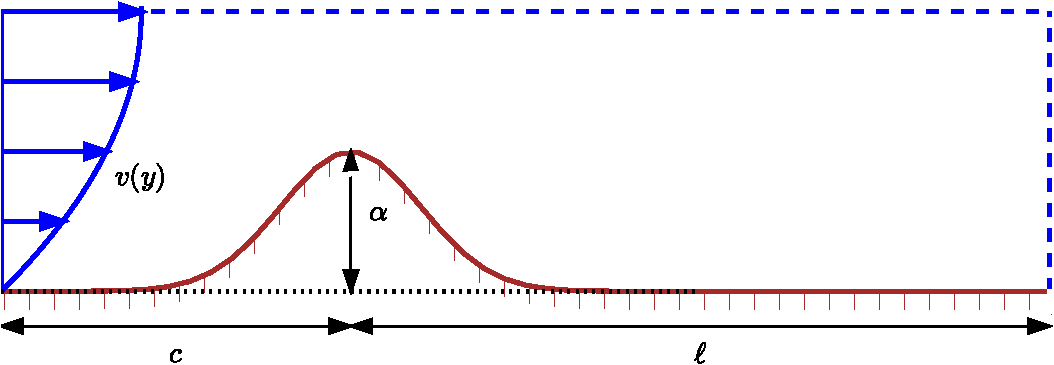
\includegraphics[width=0.9\linewidth]{fig-scaling/flow_over_gaussian.pdf}}





\vspace{3mm}




\vspace{3mm}



Inserting

\[ \bar x = \frac{x}{x_c},\ \bar y = \frac{y}{y_c},\ \bar z = \frac{z}{z_c},
\ \bar t = \frac{t}{t_c}, \ \bar\v = \frac{\v}{V},
\ \bar u =\frac{u}{u_c}\]
in (\ref{scale:convdiff:pde1}) yields

\[
\frac{u_c}{t_c}
\frac{\partial \bar u}{\partial \bar t} +
\frac{u_c V}{L}\bar\v\cdot\bar\nabla\bar u =
\frac{\dfc u_c}{L^2}\bar\nabla^2\bar u,
\quad \bar x,\bar y,\bar z\in \Omega,\ \bar t\in (0,\bar T]\tp
\]
For $u_c$ we simply introduce the symbol $U$, which we may estimate
from an initial condition. It is not critical here, since it vanishes
from the scaled equation anyway, as long as there is no source term
present.
With some velocity measure $V$ and length measure $L$, it is
tempting to just let $t_c = L/V$. This is the characteristic time it takes to
transport a signal by convection through the domain.
The alternative is to use the
diffusion length scale $t_c=L^2/\dfc$. A common physical scenario in
convection-diffusion problems is that
the convection term $\v\cdot\nabla u$ dominates over the
diffusion term $\dfc\nabla^2 u$. Therefore, the time scale for convection
($L/V$)
is most appropriate of the two. Only when
the diffusion term is very much larger than the convection
term (corresponding to very small Peclet numbers, see below)
$t_c=L^2/\dfc$ is the right time scale.

The non-dimensional form of the PDE with $t_c=L/V$ becomes

\begin{equation}
\frac{\partial \bar u}{\partial \bar t} +
\bar\v\cdot\bar\nabla\bar u =
\hbox{Pe}^{-1}\bar\nabla^2\bar u,
\quad \bar x,\bar y,\bar z\in \Omega,\ \bar t\in (0,\bar T],
\label{scale:convdiff:pde1:d}
\end{equation}
where Pe is the \emph{Peclet number},

\[ \hbox{Pe} = \frac{LV}{\dfc}\tp\]
Estimating the size of the convection term $\v\cdot\nabla u$ as
$VU/L$ and the diffusion term $\dfc\nabla^2 u$ as $\dfc U/L^2$,
we see that the Peclet number measures the ratio of the convection
and the diffusion terms:

\[ \hbox{Pe} = \frac{\hbox{convection}}{\hbox{diffusion}} =
\frac{VU/L}{\dfc U/L^2}= \frac{LV}{\dfc}\tp
\]

In case we use the diffusion time scale
$t_c=L^2/\dfc$, we get the non-dimensional PDE

\begin{equation}
\frac{\partial \bar u}{\partial \bar t} +
\hbox{Pe}\,\bar\v\cdot\bar\nabla\bar u =
\bar\nabla^2\bar u,
\quad \bar x,\bar y,\bar z\in \Omega,\ \bar t\in (0,\bar T]\tp
\label{scale:convdiff:pde1:d2}
\end{equation}


\begin{notice_mdfboxadmon}[Discussion of scales and balance of terms in the PDE]
We see that (\ref{scale:convdiff:pde1:d}) and (\ref{scale:convdiff:pde1:d2})
are not equal, and they are based on two different time scales.
For moderate Peclet numbers around 1, all terms have the same size
in (\ref{scale:convdiff:pde1:d}), i.e., a size around unity.
For large Peclet numbers,
(\ref{scale:convdiff:pde1:d}) expresses a balance
between the time derivative term and the convection term, both of size
unity, and then there is a very small
$\hbox{Pe}^{-1}\bar\nabla^2\bar u$ term because Pe is large and
$\bar\nabla^2\bar u$ should be of size unity.
That the convection term dominates over the diffusion term is
consistent with the time scale $t_c=L/V$ based on convection transport.
In this case, we can neglect the diffusion term as Pe goes to infinity
and work with a pure convection (or advection) equation

\[
\frac{\partial \bar u}{\partial \bar t} +
\bar\v\cdot\bar\nabla\bar u = 0\tp
\]

For small Peclet numbers, $\hbox{Pe}^{-1}\bar\nabla^2\bar u$ becomes
very large and can only be balanced by two terms that are supposed to
be unity of size.  The time-derivative and/or the convection term must
be much larger than unity, but that means we use suboptimal scales,
since right scales imply that $\partial\bar u/\partial\bar t$ and
$\bar v\cdot\bar\nabla\bar u$ are of order unity. Switching to a time
scale based on diffusion as the dominating physical effect gives
(\ref{scale:convdiff:pde1:d2}).  For very small Peclet numbers this
equation tells that the time-derivative balances the diffusion.
The convection term $\bar\v\cdot\bar\nabla\bar\u$ is around
unity in size, but multiplied by a very small coefficient Pe, so this term is
negligible in the PDE. An approximate PDE for small Peclet numbers is
therefore

\[
\frac{\partial \bar u}{\partial \bar t}
= \bar\nabla^2\bar u\tp
\]

Scaling can, with the above type of reasoning, be used
to neglect terms from a differential equation under precise mathematical
conditions.
\end{notice_mdfboxadmon}



\subsection{Stationary PDE}

Suppose the problem is stationary and that there is no need for
any time scale. How is this type of convection-diffusion problem
scaled? We get

\[
\frac{VU}{L}\bar\v\cdot\bar\nabla\bar u =
\frac{\dfc U}{L^2}\bar\nabla^2\bar u,
\]
or

\begin{equation}
\bar\v\cdot\bar\nabla\bar u =
\hbox{Pe}^{-1}\bar\nabla^2\bar u\tp
\label{scale:convdiff:pde1:d3}
\end{equation}
This scaling only ``works'' for moderate Peclet numbers. For very small or
very large Pe, either the convection term $\bar\v\cdot\bar\nabla\bar u$
or the diffusion term $\bar\nabla^2\bar u$ must deviate significantly
from unity.

Consider the following 1D example to illustrate the point: $\v = v\ii$,
$v>0$ constant, a domain $[0,L]$, with boundary conditions $u(0)=0$ and
$u(L)=U_L$. (The vector $\ii$ is a unit vector in $x$ direction.)
The problem with dimensions is now

\[ vu^{\prime} = \dfc u^{\prime\prime},\quad u(0)=0,\ u(L)=U_L\tp\]
Scaling results in

\[ \frac{d\bar u}{d\bar x} = \hbox{Pe}^{-1}\frac{d^2\bar u}{d\bar x^2},\quad
\bar x\in (0,1),\quad \bar u(0)=0,\ \bar u(1) = 1,\]
if we choose $U=U_L$. The solution of the scaled problem is

\[ \bar u(\bar x) = \frac{1 - e^{\bar x\hbox{\footnotesize Pe}}}{1 - e^{\hbox{\footnotesize Pe}}}\tp\]
Figure~\ref{scale:convdiff:fig:scaled} indicates how $\bar u$ depends on
Pe: small Pe values give approximately a straight line while large Pe
values lead to a \emph{boundary layer} close to $x=1$, where the solution
changes very rapidly.


\begin{figure}[!ht]  % scale:convdiff:fig:scaled
  \centerline{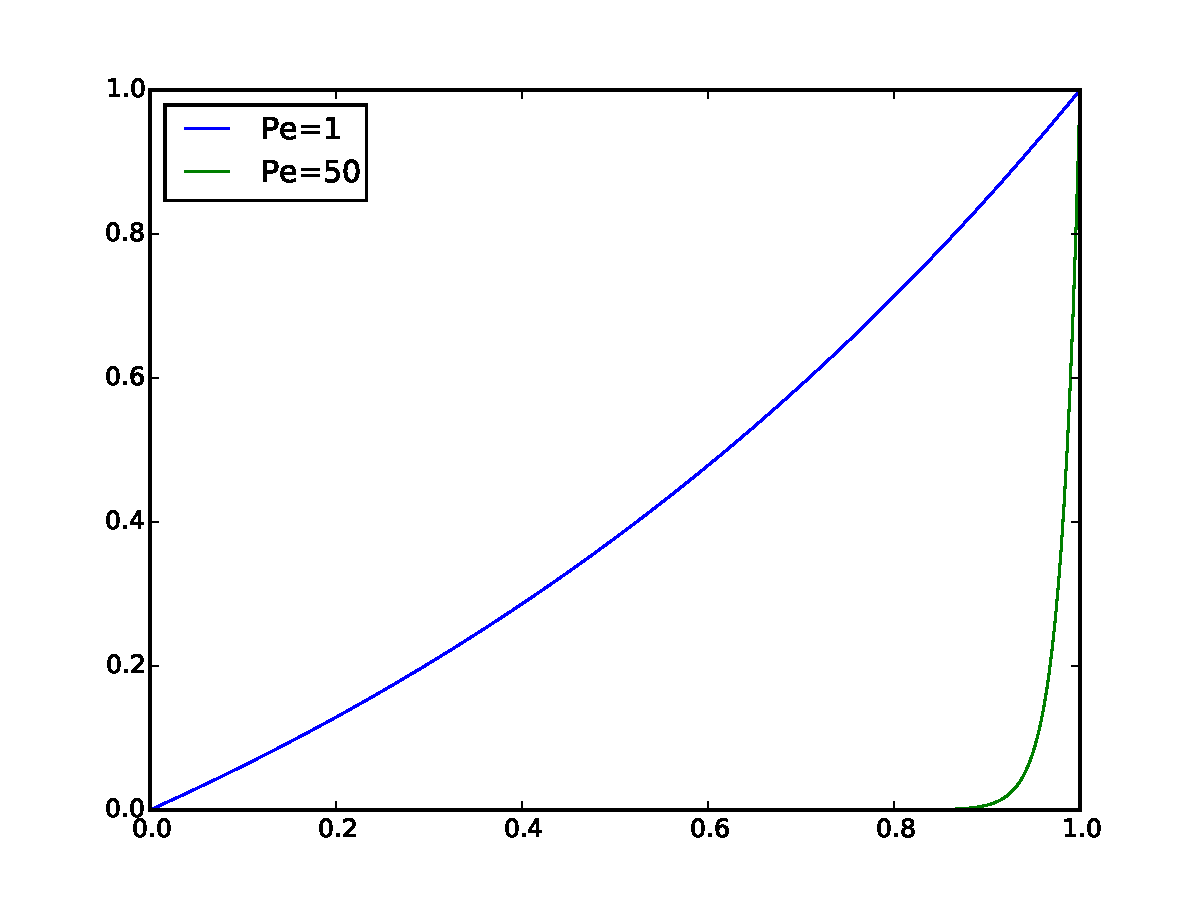
\includegraphics[width=0.9\linewidth]{fig-scaling/boundary_layer1D.pdf}}
  \caption{
  Solution of scaled problem for 1D convection-diffusion. \label{scale:convdiff:fig:scaled}
  }
\end{figure}
%\clearpage % flush figures scale:convdiff:fig:scaled


We realize that for large Pe,

\[ \max_{\bar x}\frac{d\bar u}{d\bar x} \approx \hbox{Pe},\quad
\max_{\bar x}\frac{d^2\bar u}{d\bar x^2} \approx \hbox{Pe}^{2},\]
which are consistent results with the PDE, since the double derivative term
is multiplied by $\hbox{Pe}^{-1}$.
For small Pe,

\[ \max_{\bar x}\frac{d\bar u}{d\bar x}\approx 1,\quad
   \max_{\bar x}\frac{d^2\bar u}{d\bar x^2} \approx 0,\]
which is also consistent with the PDE,
since an almost vanishing second-order derivative
is multiplied by a very large coefficient $\hbox{Pe}^{-1}$.
However, we have a problem with very large
derivatives of $\bar u$ when Pe is large.

To arrive at a proper scaling for large Peclet numbers,
we need to remove the Pe coefficient
from the differential equation. There are only two scales at our
disposals: $u_c$ and $x_c$ for $u$ and $x$, respectively.
The natural value for $u_c$ is the boundary value $U_L$ at $x=L$.
The scaling of $Vu_x = \dfc u_{xx}$ then results in

\[ \frac{d\bar u}{d\bar x} = \frac{\dfc}{Vx_c}\frac{d^2\bar u}{d\bar x^2},
\quad \bar x\in (0,\bar L),\quad \bar u(0)=0,\ \bar u(\bar L)=1,\]
where $\bar L = L/x_c$. Choosing the coefficient $\dfc/(Vx_c)$ to
be unity results in the scale $x_c=\dfc/V$, and $\bar L$ becomes Pe.
The final, scaled boundary-value
problem is now

\[ \frac{d\bar u}{d\bar x} = \frac{d^2\bar u}{d\bar x^2},
\quad \bar x \in (0, \hbox{Pe}), \quad \bar u(0)=0,\ \bar u(\hbox{Pe})=1,\]
with solution

\[ \bar u(\bar x) = \frac{1 - e^{\bar x}}{1 - e^{\hbox{\footnotesize Pe}}}\tp\]
Figure~\ref{scale:convdiff:fig:rescaled} displays $\bar u$ for some
Peclet numbers, and we see that the shape of the graphs are the same
with this scaling. For large Peclet numbers we realize that $\bar u$
and its derivatives are around unity
($1-e^{\hbox{\footnotesize Pe}}\approx -e^{\hbox{\footnotesize Pe}}$),
but for small Peclet numbers $d\bar u/d\bar x \sim \hbox{Pe}^{-1}$.


\begin{figure}[!ht]  % scale:convdiff:fig:rescaled
  \centerline{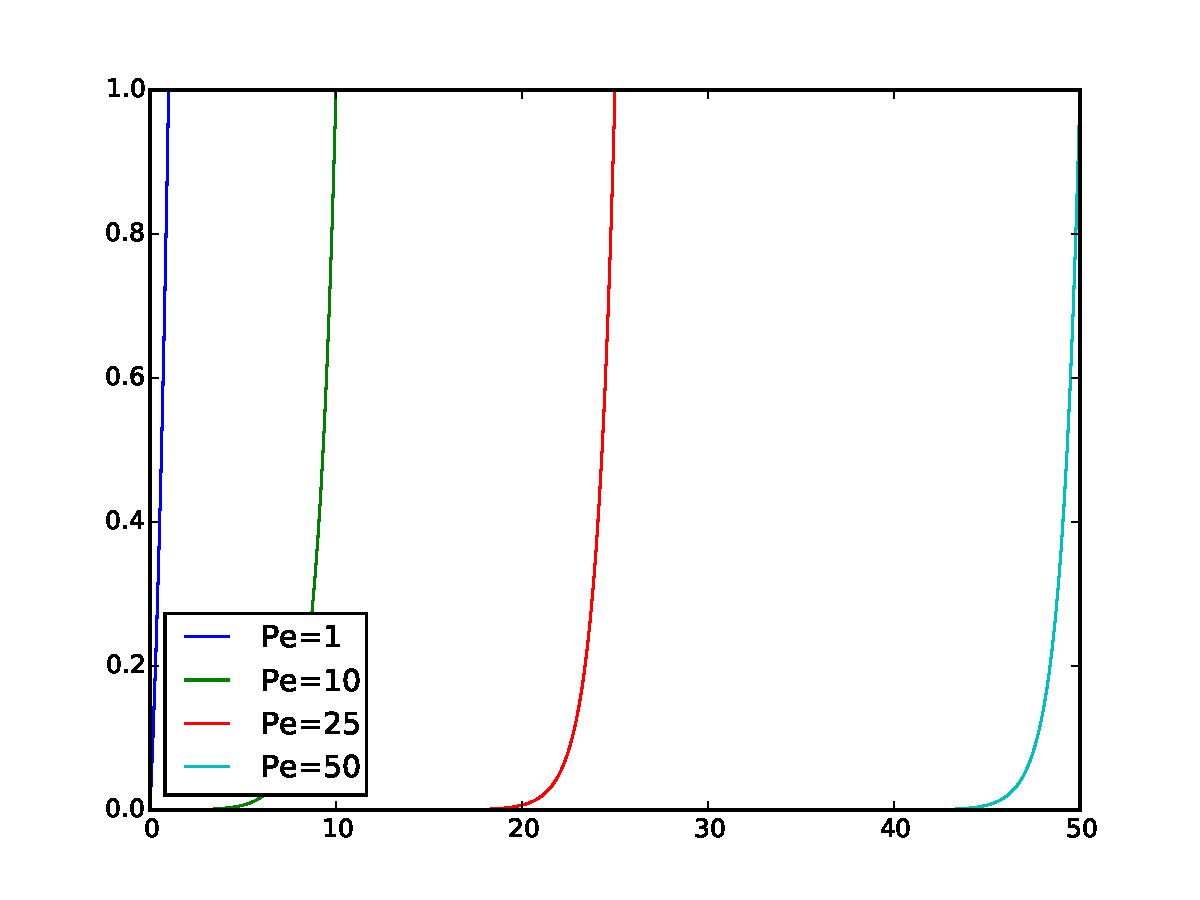
\includegraphics[width=0.9\linewidth]{fig-scaling/boundary_layer1D_scale2.pdf}}
  \caption{
  Solution of scaled problem where the length scale depends on the Peclet number. \label{scale:convdiff:fig:rescaled}
  }
\end{figure}
%\clearpage % flush figures scale:convdiff:fig:rescaled


The conclusion is that for small Peclet numbers, $x_c=L$ is an
appropriate length scale.
The scaled equation $\hbox{Pe}\,\bar u' = \bar u''$ indicates that $\bar
u''\approx 0$, and the solution is close to a straight line.  For
large Pe values, $x_c=\dfc/V$ is an appropriate length scale, and the
scaled equation $\bar u' = \bar u''$
expresses that the terms $\bar u'$ and $\bar u''$ are
equal and of size around unity.


\index{dimensionless number}
\index{Reynolds number}

\subsection{Convection-diffusion with a source term}
\label{scale:convdiff:f}

Let us add a force term $f(\x,t)$ to the convection-diffusion equation:

\begin{equation}
\frac{\partial u}{\partial t} + \v\cdot\nabla u =
\dfc\nabla^2 u + f\tp
\label{scale:convdiff:pde2}
\end{equation}
The scaled version reads

\[
\frac{\partial\bar u}{\partial\bar t} +
\frac{t_cV}{L}\bar\v\cdot\bar\nabla \bar u =
\frac{t_c\dfc}{L^2}\bar\nabla^2 \bar u +
\frac{t_cf_c}{u_c}\bar f\tp
\]
We can base $t_c$ on convective transport: $t_c = L/V$. Now,
$u_c$ could be chosen to make the coefficient in the source term unity:
$u_c = t_cf_c = Lf_c/V$.
This leaves us with

\[
\frac{\partial\bar u}{\partial\bar t} +
\bar\v\cdot\bar \nabla\bar u =
\hbox{Pe}^{-1}\bar \nabla^2 \bar u + \bar f\tp
\]

In the diffusion limit, we base $t_c$ on the diffusion time scale:
$t_c=L^2/\dfc$, and the coefficient of the source term set to unity
determines $u_c$ according to

\[ \frac{L^2 f_c}{\dfc u_c} = 1\quad\Rightarrow\quad u_c = \frac{L^2 f_c}{\dfc}\tp\]
The corresponding PDE reads

\[
\frac{\partial\bar u}{\partial\bar t} +
\hbox{Pe}\,\bar\v\cdot\bar \nabla\bar u =
\bar\nabla^2 \bar u + \bar f,
\]
so for small Peclet numbers, which we have, the convective term can
be neglected and we get a pure diffusion equation with a source term.

What if the problem is stationary?
Then there is no time scale and we get

\[
\frac{V u_c}{L}\bar\v\cdot\bar \nabla \bar u =
\frac{u_c \dfc}{L^2}\bar\nabla^2 \bar u + f_c\bar f,
\]
or

\[
\bar\v\cdot\bar \nabla \bar u =
\hbox{Pe}^{-1}\bar\nabla^2 \bar u + \frac{f_c L}{V u_c}\bar f\tp
\]
Again, choosing $u_c$ such that the source term coefficient is unity leads
to $u_c= f_c L/V$.
Alternatively, $u_c$ can be based on the initial condition, with similar
results as found in the sections on the wave and diffusion PDEs.


% !split
\chapter{Advanced partial differential equation models}

This final chapter addresses more complicated PDE models, including
linear elasticity, viscous flow, heat transfer, porous media flow,
gas dynamics, and electrophysiology. A range of
classical dimensionless numbers are discussed in terms of the scaling.

\section{The equations of linear elasticity}
\label{scale:elasticity}

To the best of the authors' knowledge, it seems that mathematical
models in elasticity and structural analysis are almost never
non-dimensionalized. This is probably due to tradition, but the
following sections will demonstrate the usefulness of scaling also in
this scientific field.

We start out with the general, time-dependent elasticity PDE with
variable material properties. Analysis based on scaling is used to
determine under what circumstances the acceleration term can be neglected
and we end up with the widely used stationary
elasticity PDE. Scaling of different types of boundary conditions is
also treated.  At the end, we scale the equations of coupled
thermo-elasticity. All the models make the assumption of small
displacement gradients and Hooke's generalized constitutive law
such that linear elasticity theory applies.

\subsection{The general time-dependent elasticity problem}
\label{scale:elasticity:timedep}

The following vector PDE governs deformation and stress in purely elastic
materials, under the assumption of small displacement gradients:

\begin{equation}
\varrho\frac{\partial^2\u}{\partial t^2} =
\nabla ((\lambda + \mu)\nabla\cdot\u) + \nabla\cdot(\mu\nabla\u) +
\varrho\f\tp
\label{scale:elasticity:PDE1}
\end{equation}
Here, $\u$ is the displacement vector,
$\varrho$ is the density of the material, $\lambda$ and $\mu$ are
the Lame elasticity parameters, and $\f$ is a body force (gravity,
centrifugal force, or similar).

We introduce dimensionless variables:

\[ \bar\u = u_c^{-1}\u,\quad \bar x = \frac{x}{L}
\quad \bar y = \frac{y}{L}
\quad \bar z = \frac{z}{L},
\quad \bar t = \frac{f}{t_c}\tp\]
Also the elasticity parameters and the density can be scaled, if they
are not constants,

\[ \bar\lambda = \frac{\lambda}{\lambda_c},\quad
\bar\mu = \frac{\mu}{\mu_c},\quad
\bar\varrho = \frac{\varrho}{\varrho_c},\]
where the characteristic quantities are typically spatial maximum values of
the functions:

\[ \lambda_c = \max_{x,y,z}\lambda,\quad
\mu_c = \max_{x,y,z}\mu,\quad
\varrho_c = \max_{x,y,z}\varrho\tp\]
Finally, we scale $\f$ too (if not constant):

\[ \bar\f = f_c^{-1}\f,\quad f_c = \max_{x,y,z,t}||\f||\tp\]

Inserting the dimensionless quantities in the governing vector PDE results in

\[
\frac{\varrho_c u_c}{t_c^2}
\frac{\partial^2\bar \u}{\partial \bar t^2} =
L^{-2}u_c\bar \nabla ((\lambda_c\bar\lambda +
\mu_c\bar\mu)\bar \nabla\cdot\bar \u) +
L^{-2}u_c\mu_c\bar \nabla\cdot(\bar \mu\bar \nabla\bar \u) +
\varrho_cf_c\bar\varrho\bar\f\tp
\]
Making the terms non-dimensional gives the equation

\begin{equation}
\bar\varrho\frac{\partial^2\bar \u}{\partial \bar t^2} =
\frac{t_c^2\lambda_c}{L^2\varrho_c}
\bar \nabla (\bar\lambda\bar\nabla\cdot\bar u) +
\frac{t_c^2\mu_c}{L^2\varrho_c}
\bar\nabla(\bar\mu \bar\nabla\cdot\bar \u) +
\frac{t_c^2\mu_c}{L^2\varrho_c}\bar \nabla\cdot(\bar \mu\bar \nabla\bar \u) +
\frac{t_c^2f_c}{u_c}\bar\varrho\bar\f\tp
\end{equation}
We may choose $t_c$ to make the coefficient in front of any of the spatial
derivative terms equal unity. Here we choose the $\mu$ term, which implies

\[ t_c = L\sqrt{\frac{\varrho_c}{\mu_c}}\tp\]
The scale for $\u$ can be chosen from an initial displacement or by
making the coefficient in front of the $\bar\f$ term unity. The latter
means

\[ u_c = \mu_c^{-1}\varrho_cf_cL^2\tp\]
As discussed later, in Section~\ref{scale:elasticity:stationary},
this might not be the desired $u_c$ in applications.

The resulting dimensionless PDE becomes

\begin{equation}
\bar\varrho\frac{\partial^2\bar \u}{\partial \bar t^2} =
\bar \nabla ((\beta\bar\lambda + \bar\mu)\bar\nabla\cdot\bar u) +
\bar \nabla\cdot(\bar \mu\bar \nabla\bar \u) +
\bar\varrho\bar\f\tp
\end{equation}
The only dimensionless parameter is

\[ \beta = \frac{\lambda_c}{\mu_c}\tp\]
If the source term is absent, we must use the initial condition or
a known boundary displacement to
determine $u_c$.

\paragraph{Software.}
Given software for (\ref{scale:elasticity:PDE1}),
we can simulate the dimensionless problem by setting $\varrho =\bar\varrho$,
$\lambda =\beta\bar\lambda$, and $\mu = \bar\mu$.


\subsection{Dimensionless stress tensor}
\label{scale:elasticity:PDE1:stress}

The stress tensor $\stress$ is a key quantity in elasticity and is given by

\[ \stress = \lambda\nabla\cdot\u\I + \mu(\nabla\u + (\nabla\u)^T)\tp\]
This $\stress$ can be computed as soon as the PDE problem for $\u$
has been solved.
Inserting dimensionless variables on the right-hand side of the above
relation gives

\begin{align*}
\stress &= \lambda_cu_cL^{-2}\bar\lambda\bar\nabla\cdot\bar\u
+ \mu_cu_cL^{-1}\bar\mu(\bar\nabla\bar\u + (\bar\nabla\bar\u)^T)\\ 
&= \mu_c u_cL^{-1}\left(\beta\bar\lambda\bar\nabla\cdot\bar\u +
\bar\mu(\bar\nabla\bar\u + (\bar\nabla\bar\u)^T)\right)\tp
\end{align*}
The coefficient on the right-hand side, $\mu_c u_cL^{-1}$, has dimension
of stress, since (according to the second table in
Section~\ref{scale:dimunit:tables}) $[\hbox{M}\hbox{T}^{-2}\hbox{L}^{-1})(\hbox{L})(\hbox{L}^{-1})]
=[\hbox{M}\hbox{T}^{-2}\hbox{L}^{-1}]$, which is the dimension of stress.
The quantity $\mu_c u_cL^{-1}$ is therefore the natural scale of the
stress tensor:

\[ \bar\stress = \frac{\stress}{\sigma_c},\quad \sigma_c = \mu_c u_c L^{-1},\]
and we have the dimensionless stress-displacement relation

\begin{equation}
\bar\stress =
\beta\bar\lambda\bar\nabla\cdot\bar\u +
\bar\mu(\bar\nabla\bar\u + (\bar\nabla\bar\u)^T)\tp
\end{equation}

\subsection{When can the acceleration term be neglected?}
\label{scale:elasticity:waves}

A lot of applications of the elasticity equation involve static or
quasi-static deformations where the acceleration term
$\varrho\u_{tt}$ is neglected. Now we shall see under which conditions
the quasi-static approximation holds.

The further discussion will need to look into the time scales of
elastic waves, because it turns out that the chosen $t_c$ above is
closely linked to the propagation speed of elastic waves in a
homogeneous body without body forces.  A relevant model for
such waves has constant
$\varrho$, $\lambda$, and $\mu$, and no force term:

\begin{equation}
\varrho\frac{\partial^2\u}{\partial t^2} =
(\lambda + \mu)\nabla \nabla\cdot\u + \mu\nabla^2\u\tp
\label{scale:elasticity:waves:eq}
\end{equation}

\paragraph{S waves.}
Let us take the curl of this PDE and notice
that the curl of a  gradient vanishes. The result is

\[\frac{\partial^2}{\partial t^2}\nabla\times\u = c_S^2\nabla^2\nabla\times\u,\]
i.e., a wave equation for $\nabla\times\u$. The wave velocity is

\[ c_S = \sqrt{\frac{\mu}{\varrho}}\tp\]
The corresponding waves are called
\href{{https://en.wikipedia.org/wiki/S-wave}}{S waves}\footnote{\texttt{https://en.wikipedia.org/wiki/S-wave}}. The curl of a
displacement field is closely related to rotation of continuum elements.
S waves are therefore rotation waves, also sometimes referred to as
shear waves.

The divergence of a displacement field can be interpreted as the
volume change of continuum elements. Suppose this volume change vanishes,
$\nabla\cdot\u = 0$, which means that the material is incompressible.
The elasticity equation then simplifies to

\[\frac{\partial^2 \u}{\partial t^2} = c_S^2\nabla^2\u,\]
\label{scale:elasticity:waves:Sweq}
so each component of
the displacement field in this case also propagates as a wave
with speed $c_S^2$.
The time it takes for such a wave to travel one characteristic length
$L$ is $L/c_S$, i.e., $L\sqrt{\varrho/\mu}$, which is nothing but
our characteristic time $t_c$.

\paragraph{P waves.}
We may take the divergence of the PDE instead and notice that $\nabla\cdot\nabla
=\nabla^2$ so

\[\frac{\partial^2}{\partial t^2}\nabla\cdot\u = c_P^2\nabla^2\nabla\cdot\u,\]
with wave velocity

\[ c_P = \sqrt{\frac{\lambda +2\mu}{\varrho}}\tp\]
That is, the volume change (expansion/compression)
propagates as a wave with speed $c_P$.
These types of waves are called \href{{https://en.wikipedia.org/wiki/P-wave}}{P waves}\footnote{\texttt{https://en.wikipedia.org/wiki/P-wave}}. Other names are pressure and expansion/compression waves.

Suppose now that $\nabla\times\u =0$, i.e., there is no rotation (``shear'') of
continuum elements. Mathematically this condition implies that
$\nabla^2\u = \nabla(\nabla\cdot\u)$ (see any book on vector calculus
or \href{{https://en.wikipedia.org/wiki/Vector_calculus_identities}}{Wikipedia}\footnote{\texttt{https://en.wikipedia.org/wiki/Vector\_calculus\_identities}}).
Our model equation (\ref{scale:elasticity:waves:eq}) then reduces to

\[ \frac{\partial^2\u}{\partial t^2} = c_P^2\nabla^2\u,\]
\label{scale:elasticity:waves:Pweq}
which is nothing but a wave equation for the expansion component of the
displacement field, just as (\ref{scale:elasticity:waves:Sweq}) is for the
shear component.


\paragraph{Time-varying load.}
Suppose we have some time-varying boundary condition on $\u$ or the
stress vector (traction), with a time scale $1/\omega$ (some
oscillating movement that goes like $\sin\omega t$, for instance). We
choose $t_c=1/\omega$.  The scaling now leads to

\[
\gamma
\frac{\partial^2\bar \u}{\partial \bar t^2} =
\bar \nabla ((\beta\bar\lambda +
\bar\mu)\bar \nabla\cdot\bar \u) +
\bar \nabla\cdot(\bar \mu\bar \nabla\bar \u) +
\bar\varrho\bar\f\tp
\]
where we have set

\[ u_c = \mu_c^{-1}f_cL^2\varrho_c,\]
as before, and $\gamma$ is a new dimensionless number,

\[ \gamma = \frac{\varrho_cL^2 \omega^2}{\mu_c} =
\left(\frac{L\sqrt{\varrho_c/\mu_c}}{1/\omega}\right)^2\tp\]
The last rewrite shows that $\sqrt{\gamma}$ is the ratio of
the time scale for S waves and the time scale for the forced
movement on the boundary. The acceleration term can therefore
be neglected when $\gamma\ll 1$, i.e., when the time scale
for movement on the boundary is much larger than the time it
takes for the S waves to travel through the domain.
Since the velocity of S waves in solids is very large and
the time scale correspondingly small, $\gamma\ll 1$
is very often the case in applications involving structural analysis.


\subsection{The stationary elasticity problem}
\label{scale:elasticity:stationary}

\paragraph{Scaling of the PDE.}
We now look at the stationary version of (\ref{scale:elasticity:PDE1})
where the $\varrho\u_{tt}$ term is removed. The first step in the
scaling is just inserting the dimensionless variables:

\[
0 =
L^{-2}u_c\bar \nabla ((\lambda_c\bar\lambda +
\mu_c\bar\mu)\bar \nabla\cdot\bar \u) +
L^{-2}u_c\mu_c\bar \nabla\cdot(\bar \mu\bar \nabla\bar \u) +
\varrho_cf_c\bar\varrho\bar\f\tp
\]
Dividing by $L^2u_c\mu_c$ gives

\[
0 =
\bar \nabla ((\beta\bar\lambda +
\bar\mu)\bar \nabla\cdot\bar \u) +
\bar \nabla\cdot(\bar \mu\bar \nabla\bar \u) +
\frac{L^2\varrho_cf_c}{u_c\mu_c}\bar\varrho\bar\f\tp
\]
Choosing $u_c = \varrho L^2f_c/\mu_c$ leads to

\begin{equation}
\bar \nabla ((\beta\bar\lambda +
\bar\mu)\bar \nabla\cdot\bar \u) +
\bar \nabla\cdot(\bar \mu\bar \nabla\bar \u) +
\bar\varrho\bar\f = 0\tp
\end{equation}

A homogeneous material with constant $\lambda$, $\mu$, and $\varrho$
is an interesting case (this corresponds to $\mu_c=\mu$, $\lambda_c=\lambda$,
$\varrho_c=\varrho$, $\bar\varrho=\bar\lambda=\bar\mu=1$):

\begin{equation}
(1+\beta)\bar \nabla(\bar \nabla\cdot\bar \u) +
\bar \nabla^2\bar \u) +
\bar\f = 0\tp
\end{equation}
Now $\beta$ is defined as

\[ \beta = \frac{\lambda}{\mu} = \left(\frac{c_p}{c_s}\right)^2 - 2\tp\]
It shows that in standard, stationary elasticity, $\lambda/\mu$ is the
only significant physical parameter.

\paragraph{Remark on the characteristic displacement.}
% The choice of $u_c$ may require a comment. If we end up with
% $\bar\u$ and a geometry of order one, it means that plotting the
% deformation (typically the deformed mesh used in a simulation) will
% look very strange.  We usually want the characteristic displacement to
% be a small fraction of the characteristic size of the elastic
% body.

The presented scaling may not be valid for problems where the geometry
involves some dimensions that are much smaller than others, such as for
beams, shells, or plates. Then more one length scale must be defined
which gives us non-dimensional geometrical numbers.  Global balances of
moments and loads then determine how characteristic displacements
depend on these numbers. As an example, consider a cantilever beam of
length $L$ and square-shaped cross section of width $W$, deformed
under its own weight.  From beam theory one can derive $u_c =
\frac{3}{2}\varrho g L^2\delta^2/E$, where $\delta = L/W$ ($g$ is the
acceleration of gravity). If we consider $E$ to be of the same size as
$\lambda$, this implies that $\gamma\sim\delta^{-2}$. So, it may be
wise to prescribe a $u_c$ in elasticity problems, perhaps from
formulas as shown, and keep $\gamma$ in the PDE.


\paragraph{Scaling of displacement boundary conditions.}
A typical boundary condition on some part of the boundary is a prescribed
displacement. For simplicity, we set $\u = \U_0$ for a constant vector
$\U_0$ as boundary condition. With $u_c=\varrho L^2f_c/\mu$, we get
the dimensionless condition

\[ \bar\u = \frac{\U_0}{u_c} = \frac{\mu \U_0}{\varrho L^2f_c}\tp\]
In the absence of body forces, the expression for $u_c$ has no
meaning ($f_c=0$), so then $u_c = |\U_0|$ is a better choice.
This gives the dimensionless boundary condition

\[ \bar u = \frac{\U_0}{|\U_0|},\]
which is the unit vector in the direction of $\U_0$. The new $u_c$
changes the coefficient in front of the body force term, if that term
is present, to the dimensionless number

\[ \delta = \frac{L^2\varrho f_c}{\mu |\U_0|}\tp\]

\paragraph{Scaling of traction boundary conditions.}
The other type of common boundary condition in elasticity is a
prescribed traction (stress vector) on some part of the boundary:

\[ \stress\cdot\normalvec = \bm{T}_0,\]
where, to make it simple, we take $\bm{T}_0$ as a constant vector.
From Section~\ref{scale:elasticity:PDE1:stress} we have a stress scale
$\sigma_c = \mu u_c/L$, but we may alternatively use $|\bm{T}_0|$
as stress scale. In that case,

\[ \bar\stress\cdot\normalvec = \frac{\bm{T}_0}{|\bm{T}_0|},\]
which is a unit vector in the direction of $\bm{T}_0$.
Many applications involve large traction free areas on the boundary, on
which we simply have $\bar\stress\cdot\normalvec = 0$.


\subsection{Quasi-static thermo-elasticity}
\label{scale:elasticity:thermo}

\index{thermo-elasticity}

Heating solids give rise to expansion, i.e., strains, which may cause
stress if displacements are constrained. The time scale of temperature
changes are usually much larger than the time scales of elastic waves,
so the stationary equations of elasticity can be used, but a term
depends on the temperature, so the equations must be coupled to
a PDE for heat transfer in solids. The resulting system of PDEs is
known as the equations of \emph{thermo-elasticity} and reads

\begin{align}
\nabla((\lambda + \mu)\nabla\cdot\u) + \nabla\cdot(\mu\nabla\u) &= \alpha\nabla T -\varrho\f,\\ 
\varrho c \frac{\partial T}{\partial t} &= \nabla\cdot(\kappa\nabla T) + \varrho \f_T,
\end{align}
where $T$ is the temperature, $\alpha$ is a coefficient of thermal expansion,
$c$ is a heat capacity, $\kappa$ is the heat conduction coefficient,
and $\f_T$ is some heat source. The density $\varrho$ is strictly speaking
a function of $T$ and the stress state, but a widely used approximation
is to consider $\varrho$ as a constant.
Most thermo-elasticity applications have
$\f_T=0$, so we drop this term. Most applications also involve some heating
from a temperature level $T_0$ to some level $T_0 +\Delta T$.
A suitable scaling for $T$ is therefore

\[ \bar T = \frac{T-T_0}{\Delta T},\]
so that $\bar T\in [0,1]$. The elasticity equation has already been scaled
and so has the diffusion equation for $T$. We base the time scale on
the diffusion, i.e., the thermal conduction process:

\[ t_c = \varrho c L^2/\kappa_c\tp\]
We imagine that $\kappa$ is scaled as $\bar\kappa = \kappa/\kappa_c$.
The dimensionless PDE system then becomes

\begin{align}
\bar \nabla((1+\beta)\bar\mu\bar\nabla\cdot\bar\u) + \bar\nabla\cdot(\bar\mu\bar\nabla\bar\u) &= \bar\nabla\bar T
-\epsilon\bar\varrho\bar\f,\\ 
\frac{\partial \bar T}{\partial \bar t} &= \bar \nabla\cdot(\bar\kappa\bar\nabla\bar T)\tp
\end{align}
Here we have chosen $u_c$ such that
the ``heating source term'' has a unit coefficient, acknowledging that
this thermal expansion balances the stress terms with $\bar\u$. The
corresponding displacement scale is

\[ u_c = \frac{\alpha L\Delta T}{\mu_c}\tp\]
The dimensionless number in the body force term is therefore

\[ \epsilon = \frac{L\varrho_c f_c}{\alpha \Delta T},\]
which measures the ratio of the body force term and the ``heating source
term''.

A homogeneous body with constant $\varrho$, $\lambda$, $\mu$, $c$, and $\kappa$
is common. The PDE system reduces in this case to

\begin{align}
\bar \nabla((1+\beta)\bar\nabla\cdot\bar\u) + \bar\nabla^2\bar\u) &= \bar\nabla\bar T -\epsilon\bar\f,\\ 
\frac{\partial \bar T}{\partial \bar t} &= \bar \nabla^2\bar T\tp
\end{align}
In the absence of body forces, $\beta$ is again the key parameter.

The boundary conditions for thermo-elasticity consist of the conditions
for elasticity and the conditions
for diffusion. Scaling of such conditions are discussed in
Section~\ref{sec:scale:diffu} and~\ref{scale:elasticity:stationary}.


\section{The Navier-Stokes equations}
\label{sec:scale:ns}

\index{Navier-Stokes equations}

This section shows how to scale various versions of the
equations governing incompressible viscous fluid flow. We start
with the plain Navier-Stokes equations without body forces and
progress with adding the gravity force and a free surface. We
also look at scaling low Reynolds number flow and oscillating flows.

\subsection{The momentum equation without body forces}

\index{dimensionless number}
\index{Reynolds number}

The Navier-Stokes equations for incompressible viscous fluid flow,
without body forces, take the form

\begin{align}
\varrho\left(\frac{\partial \u}{\partial t} + \u\cdot\nabla\u\right)
&= -\nabla p + \mu\nabla^2\u,
\label{scale:fluid:NS:eq:momentum}\\ 
\nabla\cdot\u & = 0\tp
\label{scale:fluid:NS:eq:cont}
\end{align}
The primary unknowns are the
velocity $\u$ and the pressure $p$. Moreover,
$\varrho$ is the fluid density, and $\mu$ is the dynamic viscosity.

\paragraph{Scaling.}
We start, as usual, by introducing a notation for
dimensionless independent and dependent variables:

\[ \bar x = \frac{x}{L},\quad \bar y = \frac{y}{L},\quad
\bar z= \frac{z}{L},\quad \bar t = \frac{t}{t_c},\quad
\bar\u = \frac{\u}{u_c},\quad \bar p = \frac{p}{p_c},\]
where $L$ is some characteristic distance,
$t_c$ is some characteristic time, $u_c$ is a characteristic
velocity, while $p_c$ is a characteristic pressure.
Inserted in the equations,

\begin{align}
\varrho\left(\frac{u_c}{t_c}\frac{\partial \bar\u}{\partial \bar t} + \frac{u_c^2}{L}\bar\u\cdot\bar\nabla\bar\u\right)
&= -\frac{p_c}{L}\bar\nabla\bar p + \frac{u_c}{L^2}\mu\bar \nabla^2\bar\u,
\label{scale:fluid:NS:eq:momentum_d0}\\ 
\frac{u_c}{L}\bar\nabla\cdot\bar\u & = 0\tp
\label{scale:fluid:NS:eq:cont_d0}
\end{align}
For the velocity it is common to just introduce some $U$ for
$u_c$. This $U$ is normally implied by the problem description.  For
example, in the flow configuration below, with flow over a bump, we
have some incoming flow with a profile $v(y)$ and $U$ can typically be
chosen as $U=\max_y v(y)$. The height of the bump influences the wake
behind the bump, and is the length scale that really impacts the flow,
so it is natural to set $L=D$. For numerical simulations in a domain
of finite extent, $[0,c+\ell]$, $c$ must be large enough to avoid
feedback on the inlet profile, and $\ell$ must be large enough for the
type of outflow boundary condition used.  Ideally,
$c,\ell\rightarrow\infty$, so none of these parameters are useful as
length scales.



\vspace{3mm}




\vspace{3mm}





% inline figure
\centerline{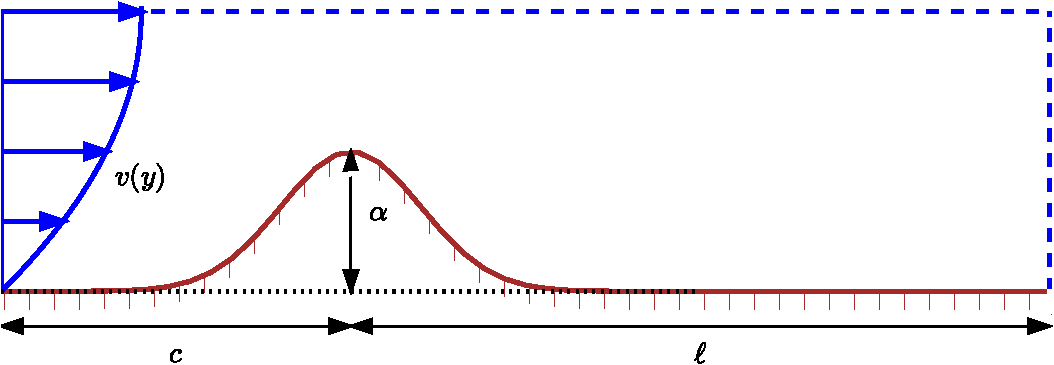
\includegraphics[width=0.9\linewidth]{fig-scaling/flow_over_gaussian.pdf}}





\vspace{3mm}




\vspace{3mm}



For flow in a channel or tube, we also have some inlet profile, e.g.,
$v(r)$ in a tube, where $r$ is the radial coordinate. A natural
choice of characteristic velocity is $U=v(0)$ or to let $U$ be
the average flow, i.e.,

\[ U = \frac{1}{\pi R^2}\int_0^R 2\pi v(r)rdr,\]
if $R$ is the radius of the tube. Other examples may be flow around
a body, where there is some distant constant inlet flow $\u = U_0\ii$,
for instance, and $U=U_0$ is an obvious choice. We therefore
assume that the flow problem itself brings a natural candidate for $U$.

Having a characteristic distance $L$ and velocity $U$, an obvious
time measure is $L/U$ so we set $t_c=L/U$. Dividing by the
coefficient in front of the time derivative term, creates a pressure
term

\[ \frac{p_c}{\varrho U^2}\bar\nabla\bar p\tp\]
The coefficient suggest a choice $p_c=\varrho U^2$ if the pressure
gradient term is to have the same size as the acceleration terms.
This $p_c$ is a very common pressure scale in fluid mechanics,
arising from Bernoulli's equation

\index{Bernoulli's equation}

\[ p + \frac{1}{2}\varrho \u\cdot\u =
\hbox{const}\]
for stationary flow.

\index{Reynolds number}

\paragraph{Dimensonless PDEs and the Reynolds number.}
The discussions so far results in the following dimensionless form of
(\ref{scale:fluid:NS:eq:momentum}) and (\ref{scale:fluid:NS:eq:cont}):

\begin{align}
\frac{\partial \bar\u}{\partial \bar t} +
\bar\u\cdot\bar\nabla\bar\u
&= -\bar\nabla\bar p + \hbox{Re}^{-1}\bar\nabla^2\bar\u,
\label{scale:fluid:NS:eq:momentum_d1}\\ 
\bar\nabla\cdot \bar\u &= 0,
\end{align}
where Re is the famous \emph{Reynolds number},

\[ \hbox{Re}= \frac{\varrho UL}{\mu} = \frac{UL}{\nu}\tp\]
The latter expression makes use of the kinematic viscosity $\nu = \mu/\varrho$.
For viscous fluid flows without body forces there is hence only one
dimensionless number, Re.

The Reynolds number can be interpreted as the ratio of convection and
viscosity:

\[ \frac{\hbox{convection}}{\hbox{viscosity}} =
\frac{|\varrho\u\cdot\nabla\u|}{|\mu\nabla^2\u|}\sim
\frac{\varrho U^2/L}{\mu U/L^2} =
\frac{UL}{\nu} = \hbox{Re}\tp\]
(We have here used that $\nabla\u$ goes like $U/L$ and $\nabla^2\u$
goes like $U/L^2$.)

\index{low Reynolds number flow}
\index{Stokes problem}

\subsection{Scaling of time for low Reynolds numbers}

As we discussed in Section~\ref{scale:convdiff} for the convection-diffusion
equation, there is not just one scaling that fits all problems.
Above, we used $t_c=L/U$, which is appropriate if convection is
a dominating physical effect. In case the convection term
$\varrho\u\cdot\nabla\u$
is much smaller
than the viscosity term $\mu\nabla^2\u$, i.e., the Reynolds number
is small, the viscosity term is dominating. However,
if the scaling is right, the other terms are of order unity, and
$\hbox{Re}^{-1}\nabla^2\bar\u$ must then also be of unit size. This fact
implies that $\nabla^2\bar\u$ must be small, but then the scaling is
not right (since a right scaling will lead to $\bar u$ and its derivatives
around unity). Such reasoning around inconsistent size of terms clearly points
to the need for other scales.

In the low-Reynolds number regime, the diffusion effect
of $\nabla^2\bar\u$ is dominating, and we should use a time scale
based on diffusion rather than convection. Such a time scale is
$t_c = L^2/(\mu/\varrho) = L^2/\nu$.
With this time scale, the dimensionless Navier-Stokes equations look like

\begin{align}
\frac{\partial \bar\u}{\partial \bar t} +
\hbox{Re}\,\bar\u\cdot\bar\nabla\bar\u
&= -\bar\nabla p + \bar\nabla^2\bar\u,
\label{scale:fluid:NS:eq:momentum_d2}\\ 
\bar\nabla\cdot\bar\u &= 0\tp
\end{align}
As stated in the box in Section~\ref{scale:convdiff}, (\ref{scale:fluid:NS:eq:momentum_d2}) is the appropriate PDE for very low Reynolds number flow and
suggests neglecting the convection term.
If the flow is also steady, the time derivative term can be neglected,
and we end up with the so-called \emph{Stokes problem} for steady, slow, viscous
flow:

\begin{align}
-\bar\nabla p + \bar\nabla^2\bar\u &= 0,
\label{scale:fluid:NS:eq:momentum_d3}\\ 
\bar\nabla\cdot\bar\u &= 0\tp
\end{align}
This flow regime is also known as \emph{Stokes' flow} or \emph{creeping flow}.

\index{Stokes' flow}
\index{Froude number}
\index{creeping flow}

\subsection{Shear stress as pressure scale}

Instead of using the kinetic energy $\varrho U^2$ as pressure scale,
one can use the shear stress $\mu U/L$ ($U/L$ reflects the spatial
derivative of the velocity, which enters the shear stress expression
$\mu\partial u/\partial y$). Using $U$ as velocity scale, $L/U$ as
time scale, and $\mu U/L$ as pressure scale, results in

\begin{equation}
\hbox{Re}\left(\frac{\partial \bar\u}{\partial \bar t} +
\bar\u\cdot\bar\nabla\bar\u\right)
= -\bar\nabla\bar p + \bar\nabla^2\bar\u\tp
\end{equation}
Low Reynolds number flow now suggests neglecting both acceleration terms.


\subsection{Gravity force and the Froude number}

We now add a gravity force to the momentum equation
(\ref{scale:fluid:NS:eq:momentum}):

\begin{equation}
\varrho\left(\frac{\partial \u}{\partial t} + \u\cdot\nabla\u\right)
= -\nabla p + \mu\nabla^2\u - \varrho g\kk,
\label{scale:fluid:NS:eq:momentum_g}
\end{equation}
where $g$ is the acceleration of gravity, and $\kk$ is a unit
vector in the opposite direction of gravity. The new term
takes the following form after non-dimensionalization:

\[ \frac{t_c}{\varrho  u_c}\varrho g \kk =  \frac{Lg}{U^2}\kk
= \hbox{Fr}^{-2}\kk,\]
where Fr is the dimensionless Froude number,

\[ \hbox{Fr} = \frac{U}{\sqrt{Lg}}\tp\]
This quantity reflects the ratio of inertia and gravity forces:

\[ \frac{|\u\cdot\nabla\u|}{|\varrho g|} \sim \frac{\varrho U^2/L}{\varrho g}
= \hbox{Fr}^2\tp\]


\subsection{Oscillating boundary conditions and the Strouhal number}

\index{Strouhal number}

Many flows have an oscillating nature, often arising from some
oscillating boundary condition. Suppose such a condition, at some
boundary $x=\hbox{const}$, takes the specific form

\[ \u = U\sin(\omega t)\ii\tp\]
The dimensionless counterpart becomes

\[ U\bar\u = U\sin(\omega \frac{L}{U}\bar t)\ii,\]
if $t_c=L/U$ is the appropriate time scale. This condition can be
written

\begin{equation}
\bar\u = \sin(\hbox{St}\,\bar t),
\end{equation}
where St is the \emph{Strouhal number},

\begin{equation}
\hbox{St} = \frac{\omega L}{U}\tp
\end{equation}
The two important dimensionless parameters in oscillating flows are
then the Reynolds and Strouhal numbers.

\index{vortex shedding}

Even if the boundary conditions
are of steady type, as for flow around a sphere or cylinder,
the flow may at certain Reynolds numbers get unsteady and oscillating.
For $10^2 < \hbox{Re} < 10^7$, steady inflow towards a cylinder will
cause vortex shedding: an array of vortices are periodically shedded
from the cylinder, producing an oscillating flow pattern and force
on the cylinder. The Strouhal number is used to characterize the
frequency of oscillations. The phenomenon, known as \emph{von Karman
vortex street}, is particularly important if the frequency
of the force on the cylinder hits the free vibration frequency
of the cylinder such that resonance occurs. The result can be large
displacements of the cylinder and structural failure. A famous
case in engineering is the failure of the \href{{https://en.wikipedia.org/wiki/Tacoma_Narrows_Bridge_(1940)}}{Tacoma Narrows suspension
bridge}\footnote{\texttt{https://en.wikipedia.org/wiki/Tacoma\_Narrows\_Bridge\_(1940)}}
in 1940, when wind-induced vortex shedding caused resonance
with the free torsional vibrations of the bridge.

\index{Euler number}

\subsection{Cavitation and the Euler number}

The dimensionless pressure in (\ref{scale:fluid:NS:eq:momentum_d1})
made use of the pressure scale $p_c=\varrho U^2$. This is an
appropriate scale if the pressure level is not of importance, which
is very often the case since only the pressure \emph{gradient} enters
the flow equation and drives the flow. However, there are circumstances
where the pressure level is of importance. For example, in some flows
the pressure may become so low that the vapor pressure of the liquid
is reached and that vapor cavities form (a phenomenon known as
\emph{cavitation}). A more appropriate pressure scale is then
$p_c = p_{\infty} - p_v$, where $p_\infty$ is a characteristic
pressure level far from vapor cavities and $p_v$ is the vapor pressure.
The coefficient in front of the dimensionless pressure gradient is then

\[ \frac{p_{\infty} - p_v}{\varrho U^2}\tp \]
Inspired by Bernoulli's equation
$p + \frac{1}{2}\varrho \u\cdot\u =
\hbox{const}$
in fluid mechanics, a factor $\frac{1}{2}$ is often inserted in the
denominator. The corresponding dimensionless number,

\begin{equation}
\hbox{Eu} = \frac{p_{\infty} - p_v}{\frac{1}{2}\varrho U^2},
\end{equation}
is called the \emph{Euler number}. The pressure gradient term now reads
$\frac{1}{2}\hbox{Eu}\,\bar\nabla\bar p$. The Euler number
expresses the ratio of pressure differences and the kinetic
energy of the flow.


\subsection{Free surface conditions and the Weber number}
\label{freesurface:Weber}
At a free surface, $z=\eta(x,y,t)$, the boundary conditions are

\begin{align}
w &= \frac{\partial\eta}{\partial t} + \u\cdot\nabla\eta,\\ 
p - p_0 & \approx
-\sigma\left(\frac{\partial^2\eta}{\partial x^2} +
\frac{\partial^2\eta}{\partial y^2}\right),
\label{scale:fluid:NS:surface_tension}
\end{align}
where $w$ is the velocity component in the $z$ direction,
$p_0$ is the atmospheric air pressure at the surface,
and $\sigma$ represents the surface tension.
The approximation in (\ref{scale:fluid:NS:surface_tension}) is valid
under small deformations of the surface.

\index{Weber number}

The dimensionless form of these conditions starts with inserting the
dimensionless quantities in the equations:

\begin{align*}
u_c\bar w &= \frac{L}{t_c}
\frac{\partial\bar\eta}{\partial\bar t} +
u_c\bar\u\cdot\bar\nabla\bar\eta,\\ 
p_c \bar p &\approx
-\frac{1}{L}\sigma\left(\frac{\partial^2\bar\eta}{\partial \bar x^2} +
\frac{\partial^2\bar\eta}{\partial \bar y^2}\right)\tp
\end{align*}
The characteristic length $L$ is usually taken as the depth of the fluid
when the surface is flat. We have used
$\bar p = (p - p_0)/p_c$ for making the pressure dimensionless.
Using $u_c=U$, $t_c=L/U$, and $p_c = \varrho U^2$, results in

\begin{align}
\bar w &= \frac{\partial\bar\eta}{\partial\bar t} +
\bar\u\cdot\bar\nabla\bar\eta,\\ 
\bar p &\approx
- \hbox{We}^{-1}\left(\frac{\partial^2\bar\eta}{\partial \bar x^2} +
\frac{\partial^2\bar\eta}{\partial \bar y^2}\right),
\label{scale:fluid:NS:surface_tension2}
\end{align}
where We is the \emph{Weber number},

\begin{equation}
\hbox{We} = \frac{\varrho U^2L}{\sigma}\tp
\end{equation}
The Weber number measures the importance of surface tension effects and
is the ratio of the pressure scale $\varrho U^2$ and the surface
tension force per area, typically $\sigma/R_x$ in a 2D problem, which
has size $\sigma/L$.

\section{Thermal convection}

Temperature differences in fluid flow cause density differences, and since
cold fluid is heavier than hot fluid, the gravity force will induce
flow due to density differences. This effect is called free thermal
convection and is key to our weather and heating of rooms.
Forced convection refers to the case where there is no
feedback from the temperature field to the motion, i.e., temperature
differences do not create motion. This fact decouples the energy
equation from the mass and momentum equations.

\subsection{Forced convection}

\index{forced convection}
\index{Peclet number}
\index{Reynolds number}

The model governing forced convection consists of the Navier-Stokes
equations and the energy equation for the temperature:

\begin{align}
\varrho\left(\frac{\partial \u}{\partial t} + \u\cdot\nabla\u\right)
&= -\nabla p + \mu\nabla^2\u - \varrho g\kk,
\label{scale:fluid:forced_convection:eq:momentum_T_forced}\\ 
\nabla\cdot\u & = 0,
\label{scale:fluid:forced_convection:eq:cont_T_forced}\\ 
\varrho c\left(\frac{\partial T}{\partial t} + \u\cdot\nabla T\right)
&= \kappa\nabla^2 T\tp
\label{scale:fluid:forced_convection:eq:energy_T_forced}
\end{align}
The symbol $T$ is the temperature, $c$ is a heat capacity, and $\kappa$
is the heat conduction coefficient for the fluid. The PDE system
applies primarily for liquids. For gases one may need a term
$- p\nabla\cdot\u$ for the pressure work in
(\ref{scale:fluid:forced_convection:eq:energy_T_forced})
as well as a modified equation of continuity
(\ref{scale:fluid:forced_convection:eq:cont_T_forced}).

Despite the fact that $\varrho$ depends on $T$, we treat $\varrho$
as a constant $\varrho_0$. The major effect of the $\varrho(T)$
dependence is through the
buoyancy effect caused by the gravity term $-\varrho(T)g\kk$.
It is common to drop this
term in forced convection,
and assume the momentum and continuity equations to be
independent of the temperature. The flow is driven by boundary
conditions (rather than density variations as in free convection),
from which we can find a characteristic velocity $U$.

Dimensionless parameters are introduced as follows:

\[ \bar x = \frac{x}{L},
\ t_c = \frac{L}{U},\ 
\bar\u = \frac{\u}{U},\ \bar p = \frac{p}{\varrho_0 U^2},\ 
\bar T = \frac{T-T_0}{T_c}\tp\]
Other coordinates are also scaled by $L$.
The characteristic temperature $T_c$ is chosen as some range $\Delta T$,
which depends on the problem and is often given by the
thermal initial and/or
boundary conditions. The reference temperature $T_0$ is also
implied by prescribed conditions.
Inserted in the equations, we get

\begin{align*}
\varrho_0\frac{U^2}{L}\frac{\partial \bar\u}{\partial \bar t} +
\varrho_0\frac{U^2}{L}\bar \u\cdot\bar \nabla\bar\u
&= -\frac{\varrho_0 U^2}{L}\bar\nabla \bar p + \frac{\mu U}{L^2}
\bar \nabla^2\bar \u,
\\ 
\frac{U}{L}\bar\nabla\cdot\bar\u & = 0,
\\ 
\varrho_0 c\left(\frac{T_c U}{L}
\frac{\partial \bar T}{\partial \bar t} +
\frac{UT_c}{L}\bar\u\cdot\bar\nabla \bar T\right)
&= \frac{\kappa T_c}{L^2}
\bar \nabla^2 \bar T \tp
\end{align*}
Making each term in each equation dimensionless reduces the system to

\begin{align}
\frac{\partial \bar\u}{\partial \bar t} +
\bar \u\cdot\bar \nabla\bar\u
&= -\bar\nabla \bar p + \hbox{Re}^{-1}\bar \nabla^2\bar \u,
\label{scale:fluid:forced_convection:eq:momentum_TB0}\\ 
\bar\nabla\cdot\bar\u & = 0,
\label{scale:fluid:forced_convection:eq:cont_TB0}\\ 
\frac{\partial \bar T}{\partial \bar t} +
\bar\u\cdot\bar\nabla \bar T
&= \hbox{Pe}^{-1}
\bar \nabla^2 \bar T\tp
\label{scale:fluid:forced_convection:eq:energy_TB0}
\end{align}

The two dimensionless numbers in this system are given by
\[
\hbox{Pe} = \frac{\varrho_0 c UL}{\kappa },\quad
\hbox{Re} = \frac{UL}{\nu}\quad (\nu = \frac{\mu}{\varrho_0})\tp
\]
The Peclet number is here defined as the ratio of the
convection term for heat $\varrho_0 c U\Delta T/L$ and the
heat conduction term $\kappa U/L^2$. The fraction
$\kappa/(\varrho_0 c)$ is known as the thermal diffusivity,
and if this quantity is given a symbol $\dfc$, we realize the
relation to the Peclet number defined in Section~\ref{scale:convdiff}.


\subsection{Free convection}
\label{scale:fluid:forced_convection}

\index{free convection}

\paragraph{Governing equations.}
The mathematical model for free thermal convection
consists of the Navier-Stokes equations
coupled to an energy equation governing the temperature:

\begin{align}
\varrho\left(\frac{\partial \u}{\partial t} + \u\cdot\nabla\u\right)
&= -\nabla p + \mu\nabla^2\u - \varrho g\kk,
\label{scale:fluid:free_convection:eq:momentum_T}\\ 
\frac{\partial\rho}{\partial t} + \nabla\cdot(\varrho\u) & = 0,
\label{scale:fluid:free_convection:eq:cont_T}\\ 
\varrho c\left(\frac{\partial T}{\partial t} + \u\cdot\nabla T\right)
&= \kappa\nabla^2 T + 2\mu\varepsilon_{ij}\varepsilon_{ij},
\label{scale:fluid:free_convection:eq:energy_T}
\end{align}
where Einstein's summation convention is implied for the
$\varepsilon_{ij}\varepsilon_{ij}$ term.[[[
The symbol $T$ is the temperature, $c$ is a heat capacity, $\kappa$
is the heat conduction coefficient for the fluid. In free convection,
the gravity term $-\varrho(T) g\kk$ is essential since the flow is driven
by temperature differences and the fact that hot fluid rises while
cold fluid falls.

For slightly compressible gas flow a term $-p\nabla\cdot\u$ may be
needed in (\ref{scale:fluid:free_convection:eq:energy_T}) and also
a modified (\ref{scale:fluid:free_convection:eq:cont_T}).

\paragraph{Heating by viscous effects.}
We have also included heating of the fluid due to the work of viscous forces,
represented by the term $2\mu\varepsilon_{ij}\varepsilon_{ij}$, where
$\varepsilon_{ij}$ is the strain-rate tensor in the flow, defined by

\[ \varepsilon_{ij} = \frac{1}{2}\left(\frac{\partial u_i}{\partial x_j}
+ \frac{\partial u_j}{\partial x_i}\right) = \frac{1}{2}(\nabla\u + (\nabla\u)^T),\]
where $u_i$ is the velocity in direction of $x_i$ ($i=1,2,3$ measures
the space directions). The term $2\mu\varepsilon_{ij}\varepsilon_{ij}$
is actually much
more relevant for forced convection, but was left out in Section~\ref{scale:fluid:forced_convection} for mathematical simplicity.
Heating by the work of viscous forces is often a very small effect and
can be neglected, although it plays a major role in forging and
extrusion of metals where the viscosity is very large (such
processes require large external forces to drive the flow).  The reason
for including the work by viscous forces under the heading
of free convection, is that we want to scale a more complete,
general mathematical model for mixed force and free convection, and
arrive at dimensionless numbers that can tell if this extra term is
important or not.

\paragraph{Relation between density and temperature.}
The equations (\ref{scale:fluid:free_convection:eq:momentum_T}) and
(\ref{scale:fluid:free_convection:eq:cont_T}) has already been made dimensionless
in the previous section. The major difference is now that $\varrho$
is no longer a constant, but a function of $T$.
The relationship between $\varrho$ and $T$ is often taken as
linear,

\[ \varrho = \varrho_0 -\varrho_0 \beta (T-T_0),\]
where

\[ \beta = -\frac{1}{\varrho}\left(\frac{\partial\varrho}{\partial t}
\right)_p,\]
is known as the thermal expansion coefficient of the fluid,
and $\varrho_0$ is a reference density when the temperature is at $T_0$.


\paragraph{The Boussinesq approximation.}
A very common approximation, called the \emph{Boussinesq approximation}, is
to neglect the density variations in all terms except the gravity term.
This is a good approximation unless the change in $\varrho$ is large.
With the linear $\varrho(T)$ formula and the Boussinesq approximation,
(\ref{scale:fluid:free_convection:eq:momentum_T})-(\ref{scale:fluid:free_convection:eq:energy_T})
take the form

\begin{align}
\varrho_0\left(\frac{\partial \u}{\partial t} + \u\cdot\nabla\u\right)
&= -\nabla p + \mu\nabla^2\u - (\varrho_0 - \varrho_0\beta(T-T_0))g\kk,
\label{scale:fluid:free_convection:eq:momentum_TB}\\ 
\nabla\cdot\u & = 0,
\label{scale:fluid:free_convection:eq:cont_TB}\\ 
\varrho_0 c\left(\frac{\partial T}{\partial t} + \u\cdot\nabla T\right)
&= \kappa\nabla^2 T + 2\mu\varepsilon_{ij}\varepsilon_{ij}\tp
\label{scale:fluid:free_convection:eq:energy_TB}
\end{align}
A good justification of the Boussinesq approximation is provided
by Tritton \cite[Ch.~13]{Tritton}.

\paragraph{Scaling.}
Dimensionless variables are introduced as

\[ \bar x = \frac{x}{L},\ \ t_c = \frac{L}{U},\ 
\bar\u = \frac{\u}{U},\ \bar p = \frac{p}{\varrho U^2},\ 
\bar T = \frac{T-T_0}{\Delta T}\tp\]
The dimensionless $y$ and $z$ coordinates also make use of $L$ as scale.
As in forced convection, we assume the characteristic temperature
level $T_0$ and the scale $\Delta T$ are given by thermal boundary and/or
initial conditions.
Contrary to Sections~\ref{sec:scale:ns} and~\ref{scale:fluid:forced_convection},
$U$ is now not given by the problem description, but implied by
$\Delta T$.

Replacing quantities with dimensions by their dimensionless counterparts
results in

\begin{align*}
\varrho_0\frac{U^2}{L}\frac{\partial \bar\u}{\partial \bar t} +
\varrho_0\frac{U^2}{L}\bar \u\cdot\bar \nabla\bar\u
&= -\frac{p_c}{L}\bar\nabla \bar p + \frac{\mu U}{L^2}
\bar \nabla^2\bar \u - \varrho_0g\kk + \varrho_0\beta T_c\bar T g\kk,
\\ 
\frac{U}{L}\bar\nabla\cdot\bar\u & = 0,
\\ 
\varrho_0 c\left(\frac{T_c U}{L}
\frac{\partial \bar T}{\partial \bar t} +
\frac{UT_c}{L}\bar\u\cdot\bar\nabla \bar T\right)
&= \frac{\kappa T_c}{L^2}
\bar \nabla^2 \bar T + 2\frac{\mu U}{L}
\bar\varepsilon_{ij}\bar\varepsilon_{ij}\tp
\end{align*}
These equations reduce to

\begin{align}
\frac{\partial \bar\u}{\partial \bar t} +
\bar \u\cdot\bar \nabla\bar\u
&= -\bar\nabla \bar p + \hbox{Re}^{-1}\bar \nabla^2\bar \u
- \hbox{Fr}^{-2}\kk  + \gamma \bar T\kk,
\label{scale:fluid:free_convection:eq:momentum_TB0}\\ 
\bar\nabla\cdot\bar\u & = 0,
\label{scale:fluid:free_convection:eq:cont_TB0}\\ 
\frac{\partial \bar T}{\partial \bar t} +
\bar\u\cdot\bar\nabla \bar T
&= \hbox{Pe}^{-1}\bar \nabla^2 \bar T + 2\delta
\bar\varepsilon_{ij}\bar\varepsilon_{ij}\tp
\label{scale:fluid:free_convection:eq:energy_TB0}
\end{align}

The dimensionless numbers, in addition to Re and Fr, are
\[
\gamma = \frac{g\beta L\Delta T }{U^2},\quad
\hbox{Pe}^{-1} = \frac{\kappa }{\varrho_0 c UL},\quad
\delta = \frac{\mu U}{L\varrho_0 c \Delta T}\tp
\]
The Peclet number is here defined as the ratio of the
convection term for heat $\varrho_0 c U\Delta T/L$ and the
heat conduction term $\kappa U/L^2$.
The $\gamma$ number measures the ratio of thermal buoyancy and
the convection term:

\[ \gamma = \frac{\varrho_0 g\beta \Delta T }{\varrho_0 U^2/L}
= \frac{g\beta L\Delta T }{U^2}\tp\]
The Pe parameter is the fraction of the convection term
and the thermal diffusion term:

\[ \frac{|\varrho_0\u\cdot\nabla T|}{|\kappa\nabla^2 T|}\sim
\frac{\varrho_0 c U \Delta T L^{-1}}{\kappa L^{-2}\Delta T}
= \frac{\varrho c UL}{\kappa } = \hbox{Pe}\tp\]
The $\delta$ parameter is the ratio of the viscous dissipation term
and the convection term:

\[ \frac{|\mu\nabla^2\u|}{|\varrho_0c\u\cdot\nabla T|}\sim
\frac{\mu U^2/L^2}{\varrho_0 c U \Delta T/L} =
\frac{\mu U}{L\varrho_0 c \Delta T} = \delta\tp
\]

\subsection{The Grashof, Prandtl, and Eckert numbers}

\index{Grashof number}
\index{Reynolds number}

The problem with the above dimensionless numbers is that they involve
$U$, but $U$ is implied by $\Delta T$. Assuming that the convection
term is much bigger than the viscous diffusion term, the momentum
equation features a balance between the buoyancy term and the convection
term:

\[ |\varrho_0 \u\cdot\nabla\u| \sim \varrho_0 g \beta\Delta T\tp\]
Translating this similarity to scales,

\[ \varrho_0 U^2/L \sim \varrho_0 g \beta\Delta T,\]
gives an $U$ in terms of $\Delta T$ :

\[ U = \sqrt{\beta L \Delta T}\tp\]
The Reynolds number with this $U$ now becomes

\[ \hbox{Re}_T = \frac{UL}{\nu} = \frac{\sqrt{g\beta L^3 \Delta T}}{\nu^2}
= \hbox{Gr}^{1/2},\]
where Gr is the Grashof number in free thermal convection:

\[ \hbox{Gr} = \hbox{Re}_T^2 =  \frac{g\beta L^3 \Delta T}{\nu^2}\tp\]
The Grashof number replaces the Reynolds number in the scaled equations
of free thermal convection. We shall soon look at its interpretations,
which are not as straightforward as for the Reynolds and Peclet numbers.

The above
choice of $U$ in terms of $\Delta T$ results in $\gamma$ equal to unity:

\[ \gamma = \frac{g\beta L\Delta T }{U^2} =
\frac{g\beta L\Delta T }{g\beta L \Delta T} = 1\tp\]

\index{Peclet number}

The Peclet number can also be rewritten as

\[ \hbox{Pe}= \frac{\varrho c UL}{\kappa } = \frac{\mu c}{\kappa}
\frac{\varrho UL}{\mu}
= \hbox{Pr}\hbox{Re}^{-1} = \hbox{Pr}\hbox{Re}_T^{-1},\]
where Pr is the Prandtl number, defined as

\[ \hbox{Pr} = \frac{\mu c}{\kappa}\tp\]

The Prandtl number is the ratio of the momentum diffusivity (kinematic
viscosity) and the thermal diffusivity. Actually, more detailed
analysis shows that Pr reflects the ratio of the thickness of the
thermal and velocity boundary layers: when $\hbox{Pr}=1$, these layers
coincide, while $\hbox{Pr}\ll 1$ implies that the thermal layer is
much thicker than the velocity boundary layer, and vice versa for
$\hbox{Pr}\gg 1$.

\index{Eckert number}

The $\delta$ parameter is in free convection replaced by a combination
of the Eckert number (Ec) and the Reynolds number. We have that

\[ \hbox{Ec} = \frac{U^2}{c\Delta T} = \delta\hbox{Re}_T,\]
and consequently

\[ \delta = \hbox{Ec}\hbox{Re}_T^{-1} = \hbox{Ec}\hbox{Gr}^{-1/2}\tp\]
Writing

\[ \hbox{Ec} = \frac{\varrho_0U^2}{\varrho_0c\Delta T},\]
shows that the Eckert number can be interpreted as the ratio of
the kinetic energy of the flow and the thermal energy.

We use Gr instead of $\hbox{Re}_T$ in the momentum equations and also
instead of Pe in the energy equation (recall that $\hbox{Pe} =
\hbox{Pr}\hbox{Re} =
\hbox{Pr}\hbox{Re}_T=\hbox{Pr}\hbox{Gr}^{-1/2}$). The resulting scaled
system becomes

\begin{align}
\frac{\partial \bar\u}{\partial \bar t} +
\bar \u\cdot\bar \nabla\bar\u
&= -\bar\nabla \bar p + \hbox{Gr}^{-1/2}\bar \nabla^2\bar \u
- \hbox{Fr}^{-2}\kk  + \bar T \kk,
\label{scale:fluid:free_convection:eq:momentum_TB1}\\ 
\bar\nabla\cdot\bar\u & = 0,
\label{scale:fluid:free_convection:eq:cont_TB1}\\ 
\hbox{Gr}^{1/2}\left(\frac{\partial \bar T}{\partial \bar t} +
\bar\u\cdot\bar\nabla \bar T\right)
&= \hbox{Pr}^{-1}
\bar \nabla^2 \bar T + 2\hbox{Ec}\hbox{Gr}^{-1/2}
\bar\varepsilon_{ij}\bar\varepsilon_{ij}\tp
\label{scale:fluid:free_convection:eq:energy_TB1}
\end{align}

The Grashof number plays the same
role as the Reynolds number in the momentum equation in free
convection. In particular,
it turns out that Gr governs the transition between laminar and
turbulent flow.  For example, the transition to turbulence occurs in
the range $10^8 < \hbox{Gr} < 10^9$ for free convection from vertical
flat plates.  Gr is normally interpreted as a dimensionless number
expressing the ratio of buoyancy forces and viscous forces.

\paragraph{Interpretations of the Grashof number.}
Recall that the scaling leading to the Grashof number is based on an
estimate of $U$ from a balance of the convective and the buoyancy
terms. When the viscous term dominates over convection, we need a
different estimate of $U$, since in this case, the viscous force
balances the buoyancy force:

\[ \mu\nabla^2\u \sim \varrho_0g\beta\Delta T\quad
\Rightarrow\quad \mu U/L^2 \sim \varrho_0g\beta\Delta T,\]
This similarity suggests the scale

\[ U = \frac{g\beta L^2 \Delta T}{\nu}\tp\]
Now,

\[ \frac{|\varrho_0\u\cdot\nabla\u|}{|\mu\nabla^2\u|} \sim \frac{UL}{\nu}
= \frac{g\beta L^3 \Delta T}{\nu} = \hbox{Gr}\tp\]
The result means that $\hbox{Gr}^{1/2}$ measures the ratio of convection and
viscous forces when convection dominates, whereas Gr measures this ratio when
viscous forces dominate.

The product of Gr and Pr is the Rayleigh number,

\[
\hbox{Ra} = \frac{g\beta L^3\Delta T\varrho_0 c}{\nu\kappa},
\]
since

\[
\hbox{Gr} \hbox{Pr} = \hbox{Re}_T^2\hbox{Pr} =
\frac{g\beta L^3 \Delta T}{\nu^2}\frac{\mu c}{\kappa} =
\frac{g\beta L^3 \Delta T\varrho_0 c}{\nu\kappa} =
\hbox{Ra}\tp
\]
The Rayleigh number is the preferred dimensionless number when studying
free convection in horizontal layers \cite{Drazin_Reid,Tritton}. Otherwise,
Gr and Pr are used.


\subsection{Heat transfer at boundaries and the Nusselt and Biot numbers}

\index{Nusselt number}
\index{Biot number}

A common boundary condition, modeling heat transfer to/from the
surroundings, is

\begin{equation}
-\kappa\frac{\partial T}{\partial n} = h(T - T_s),
\label{scale:fluid:free_convection:fluxcond}
\end{equation}
where $\partial/\partial n$ means the derivative in the normal direction
($\normalvec\cdot\nabla$), $h$ is an experimentally determined
heat transfer coefficient, and $T_s$ is the temperature of
the surroundings. Scaling (\ref{scale:fluid:free_convection:fluxcond})
leads to

\[ -\frac{\kappa\Delta t}{L}\frac{\partial \bar T}{\partial \bar n} = h(\Delta T \bar T + T_0 - T_s),\]
and further to

\[ \frac{\partial \bar T}{\partial \bar n} =
\frac{hL}{\kappa}(\bar T + \frac{T_s - T_0}{\Delta T})
= \delta(\bar T - \bar T_s),
\]
where the dimensionless number $\delta$ is defined by

\[ \delta = \frac{hL}{\kappa},\]
and $\bar T_s$ is simply the dimensionless surrounding temperature,

\[ \bar T_s = \frac{T_s - T_0}{\Delta T}\tp\]

When studying heat transfer in a fluid, with solid surroundings,
$\delta$ is known as the \href{{https://en.wikipedia.org/wiki/Nusselt_number}}{Nusselt number}\footnote{\texttt{https://en.wikipedia.org/wiki/Nusselt\_number}} Nu.  The left-hand side
of (\ref{scale:fluid:free_convection:fluxcond}) represents in this case
heat conduction, while the right-hand side models convective heat
transfer at a boundary. The Nusselt number can then be interpreted as
the ratio of convective and conductive heat transfer at a solid
boundary:

\[ \frac{|h(T-T_s)|}{\kappa T/L} \sim \frac{h}{\kappa /L} = \hbox{Nu}\tp\]

The case with heat transfer in a solid with a fluid as surroundings
gives the same dimensionless $\delta$, but the number is now known as
the \href{{https://en.wikipedia.org/wiki/Biot_number}}{Biot number}\footnote{\texttt{https://en.wikipedia.org/wiki/Biot\_number}}. It
describes the ratio of heat loss/gain with the surroundings at the
solid body's boundary and conduction inside the body. A small Biot
number indicates that conduction is a fast process and one can use
Newton's law of cooling (see Section~\ref{scale:cooling:const})
instead of a detailed calculation of the
spatio-temporal temperature variation in the body.

Heat transfer is a huge engineering
field with lots of experimental investigations
that are summarized by curves relating various dimensionless numbers
such as Gr, Pr, Nu, and Bi.


\section{Compressible gas dynamics}
\label{scale:gasdyn}

\subsection{The Euler equations of gas dynamics}
\label{scale:Euler_eqs}



The fundamental equations for a compressible fluid are based on balance
of mass, momentum, and energy. When molecular diffusion effects are
negligible, the PDE system, known as the Euler
equations of gas dynamics, can be written as

\begin{align}
\frac{\partial\varrho}{\partial t} + \nabla\cdot(\varrho\u) &= 0,
\label{scale:Euler_eqs:mass}\\ 
\frac{\partial(\varrho\u)}{\partial t} + \nabla\cdot(\varrho\u\u^T) &= -\nabla p + \varrho \f,
\label{scale:Euler_eqs:mom}\\ 
\frac{\partial E}{\partial t} + \nabla\cdot(\u(E+p)) &= 0,
\label{scale:Euler_eqs:energy}
\end{align}
with $E$ being

\begin{equation}
E = \varrho e + \frac{1}{2}\varrho\u\cdot\u\tp
\label{scale:Euler_eqs:E}
\end{equation}
In these equations, $\u$ is the fluid velocity, $\varrho$ is the density,
$p$ is the pressure, $E$ is the total energy per unit volume, composed
of the kinetic energy per unit volume, $\half\varrho \u\cdot\u$, and the
internal energy per unit volume, $\varrho e$.

Assuming the fluid to be an ideal gas implies the following additional
relations:

\begin{align}
e &= c_v T,
\label{scale:Euler_eqs:e}\\ 
p &= \varrho RT = \frac{R}{c_v}(E-\half\varrho \u\cdot\u),
\label{scale:Euler_eqs:p}
\end{align}
where $c_v$ is the specific heat capacity at constant volume (for dry air
$c_v = 717.5\, \hbox{J}\,\hbox{kg}^{-1}\hbox{K}^{-1}$),
$R$ is the specific ideal gas constant
($R=287.14 \hbox{J}\hbox{kg}^{-1}\hbox{K}^{-1}$), and $T$ is the temperature.

The common way to solve these equations is to propagate $\varrho$,
$\varrho\u$, and $E$ by an explicit numerical method in time for
(\ref{scale:Euler_eqs:mass})-(\ref{scale:Euler_eqs:energy}),
using (\ref{scale:Euler_eqs:p}) for $p$.


We introduce dimensionless independent variables,

\[ \bar x = \frac{x}{L},\quad \bar y = \frac{y}{L},\quad \bar z = \frac{z}{L},
\quad \bar t = \frac{t}{t_c},\]
and dimensionless dependent variables,

\[ \bar\u = \frac{\u}{U},\quad\bar\varrho = \frac{\varrho}{\varrho_c},
\quad\bar p = \frac{p}{p_c},\quad \bar E= \frac{E}{E_c}\tp\]
Inserting these expressions in the governing equations gives

\begin{align*}
\frac{\partial\bar\varrho}{\partial\bar t} + \frac{t_c U}{L}\bar\nabla\cdot(\bar\varrho\bar\u) &= 0,\\ 
\frac{\partial(\bar\varrho\bar\u)}{\partial\bar t} + \frac{t_cU}{L}\bar\nabla\cdot(\bar\varrho\bar\u\bar\u^T) &= -\frac{t_cp_c}{UL\varrho_c}\nabla\bar p + \frac{t_c f_c}{U}\bar\varrho \bar\f,\\ 
\frac{\partial\bar E}{\partial\bar t} + \frac{t_c U}{LE_c }\bar\nabla\cdot(\bar\u(E_c\bar E+p_c\bar p)) &= 0,\\ 
\bar p & = \frac{R}{c_v p_c}(E_c\bar E - \half\varrho_cu_c\bar\varrho\bar\u\cdot\bar\u)\tp
\end{align*}
A natural choice of time scale is $t_c=L/U$. A common choice of
pressure scale is $p_c=\varrho_c U^2$. The energy equation simplifies if
we choose $E_c=p_c=\varrho_c U^2$. With these scales we get

\begin{align*}
\frac{\partial\bar\varrho}{\partial\bar t} +
\bar\nabla\cdot(\bar\varrho\bar\u) &= 0,\\ 
\frac{\partial(\bar\varrho\bar\u)}{\partial\bar t} +
\bar\nabla\cdot(\bar\varrho\bar\u\bar\u^T) &=
-\nabla\bar p + \alpha\bar\varrho \bar\f,\\ 
\frac{\partial\bar E}{\partial\bar t} +
\bar\nabla\cdot(\bar\u(\bar E+ \bar p)) &= 0,\\ 
\bar p & = \frac{R}{c_v}(\bar E - \half\bar\varrho\bar u\cdot\bar u),
\end{align*}
where $\alpha$ is a dimensionless number:

\[ \alpha = \frac{Lf_c}{U^2}\tp\]
We realize that the scaled Euler equations look like
the ones with dimension, apart from the $\alpha$ coefficient.


\subsection{General isentropic flow}

Heat transfer can be neglected in
\href{{https://en.wikipedia.org/wiki/Isentropic_process}}{isentropic flow}\footnote{\texttt{https://en.wikipedia.org/wiki/Isentropic\_process}},
and there is hence an equation of state involving only $\varrho$ and
$p$:

\[ p = F(\varrho)\tp\]
The energy equation is now not needed and the Euler equations simplify
to

\begin{align}
\frac{\partial\varrho}{\partial t} + \nabla\cdot(\u\varrho) &=0,
\label{scale:gas:acoustic:rho}\\ 
\varrho\frac{\partial\u}{\partial t} + \varrho\u\cdot\nabla\u + \nabla p &=0\tp
\label{scale:gas:acoustic:u}
\end{align}

\paragraph{Elimination of the pressure.}
A common equation of state is

\[ F(\varrho) = p_0\left(\frac{\varrho}{\varrho_0}\right)^\gamma,\]
where $\gamma = 5/3$ for air. The first step is to eliminate $p$ in
favor of $\varrho$ so we get a system for $\varrho$ and $\u$.
To this end, we must calculate $\nabla p$:

\[ \nabla p = F'(\varrho)\nabla\varrho,\quad
F'(\varrho)= c_0^2\left(\frac{\varrho}{\varrho_0}\right)^{\gamma-1},\]
where

\[ c_0 = \sqrt{\frac{\gamma p_0}{\varrho_0}}\]
is the speed of sound within the fluid in the equilibrium state (see the subsequent section).
Equation (\ref{scale:gas:acoustic:u}) with eliminated pressure $p$ reads

\begin{equation}
\varrho\frac{\partial\u}{\partial t} + \varrho\u\cdot\nabla\u +
c_0^2\left(\frac{\varrho}{\varrho_0}\right)^{\gamma-1}\nabla\varrho =0\tp
\label{scale:gas:acoustic:u2}
\end{equation}

The governing equations are now (\ref{scale:gas:acoustic:rho})
and (\ref{scale:gas:acoustic:u2}).
Space and time are scaled in the usual way as

\[ \bar x = \frac{x}{L},\quad\bar y = \frac{y}{L},\quad\bar z = \frac{z}{L},
\quad\bar t = \frac{t}{t_c}\tp\]
The scaled dependent variables are

\[ \bar\varrho = \frac{\varrho}{\varrho_c},\quad \bar\u = \frac{\u}{U}\tp\]
Then $F'(\varrho)=c_0^2\bar\varrho^{\gamma-1}$.

Inserting the dimensionless variables in the two governing PDEs leads to

\begin{align*}
\frac{\varrho_c}{t_c}\frac{\partial\bar\varrho}{\partial\bar t}
+ \frac{\varrho_c U}{L}\bar\nabla\cdot(\bar\varrho\bar\u) &=0,\\ 
\frac{\varrho_c U}{t_c}\bar\varrho
\frac{\partial\bar\u}{\partial\bar t} +
\frac{\varrho_c U^2}{L}\bar\varrho\bar u\cdot\bar\nabla\bar\u
+ \frac{\varrho_c}{L}\left(\frac{\varrho_c}{\varrho_0}\right)^{\gamma-1}c_0^2\bar\varrho^{\gamma-1}
\bar\nabla\bar\varrho
&=0\tp
\end{align*}
The characteristic flow velocity is $U$ so a natural time scale is
$t_c = L/U$. This choice leads to the scaled PDEs

\begin{align}
\frac{\partial\bar\varrho}{\partial\bar t}
+ \bar\nabla\cdot(\bar\varrho\bar\u) &=0,
\label{scale:gas:acoustic:isentropic:cont:s}\\ 
\bar\varrho
\frac{\partial\bar\u}{\partial\bar t} +
\bar\varrho\bar\u\cdot\bar\nabla\bar\u
+ \hbox{M}^{-2}\left(\frac{\varrho_c}{\varrho_0}\right)^{\gamma-1}\bar\varrho^{\gamma-1}
\bar\nabla\bar\varrho
&=0,
\label{scale:gas:acoustic:isentropic:mom:s}
\end{align}
where the dimensionless number

\[ \hbox{M} = \frac{U}{c_0},\]
is known as the \emph{Mach number}.
The boundary conditions specify the characteristic velocity $U$ and
thereby the Mach number. Observe that (\ref{scale:gas:acoustic:isentropic:mom:s})
simplifies if $\varrho_c=\varrho_0$ is an appropriate choice.

\index{Mach number}


\subsection{The acoustic approximation for sound waves}
\label{scale:gas:acoustic}

\paragraph{Wave nature of isentropic flow with small perturbations.}
A model for sound waves can be based on (\ref{scale:gas:acoustic:rho})
and (\ref{scale:gas:acoustic:u2}), but in this case
there are small pressure, velocity, and
density \emph{perturbations} from a ground state at rest
where $\u=0$, $\varrho=\varrho_0$, and $p=p_0 = F(\varrho_0)$.
Introducing the perturbations $\hat\varrho = \varrho - \varrho_0$ and $\hat\u$,
(\ref{scale:gas:acoustic:rho})
and (\ref{scale:gas:acoustic:u2}) take the form

\begin{align*}
\frac{\partial\hat\varrho}{\partial t} + \nabla\cdot(\hat\u(\varrho_0 + \hat\varrho) &=0,\\ 
(\varrho_0 + \hat\varrho)
\frac{\partial\hat\u}{\partial t} + (\varrho_0+\hat\varrho)\hat\u\cdot\nabla\hat\u +
c_0^2\left(1 + \frac{\hat\varrho}{\varrho_0}\right)^{\gamma-1}\nabla\hat\varrho &=0\tp
\end{align*}
For small perturbations we can linearize this PDE system by
neglecting all products of $\hat\varrho$ and
$\hat\u$. Also, $1 + \hat\varrho/\varrho_0\approx 1$.
This leaves us with the simplified system

\begin{align*}
\frac{\partial\hat\varrho}{\partial t} + \varrho_0\nabla\cdot\hat\u &=0,\\ 
\varrho_0\frac{\partial\hat\u}{\partial t} +
c_0^2\nabla\hat\varrho &=0\tp
\end{align*}
Eliminating $\hat\u$ by differentiating the first PDE with respect to $t$
and taking the divergence of the second PDE gives a standard wave equation
for the density perturbations:

\[ \frac{\partial^2\hat\varrho}{\partial t^2} = c_0^2\nabla^2\hat\varrho\tp\]
Similarly, $\hat\varrho$ can be eliminated and one gets a wave equation for
$\hat\u$, also with wave velocity $c_0$.
This means that the sound perturbations travel with velocity $c_0$.


\paragraph{Basic scaling for small wave perturbations.}
Let $\varrho_c$ and
$u_c$ be characteristic sizes of the perturbations in density and velocity.
The density will then vary in $[\varrho_0-\varrho_c,\varrho_0+\varrho_c]$.
An appropriate scaling is

\[ \bar\varrho =\frac{\varrho - \varrho_0}{\varrho_c} \]
such that $\bar\varrho\in [-1,1]$. Consequently,

\[ \varrho = \varrho_0 + \varrho_c\bar\varrho = \varrho_0(1 + \alpha\bar\varrho),\quad \alpha = \frac{\varrho_c}{\varrho_0}\tp\]
Note that the dimensionless $\alpha$ is expected to be a very small number
since $\varrho_c\ll \varrho_0$.
The velocity, space, and time are scaled as in the previous
section.
Also note that $\varrho_0$ and $p_0$ are known values, but the scales
$\varrho_c$ and $U$ are not known. Usually these
can be estimated from perturbations (i.e., sound generation)
applied at the boundary.

Inserting the scaled variables in (\ref{scale:gas:acoustic:rho})
and (\ref{scale:gas:acoustic:u2}) results in

\begin{align*}
\alpha\frac{\varrho_0}{t_c}\frac{\partial\bar\varrho}{\partial\bar t}
+ \frac{\varrho_0 U}{L}\bar\nabla\cdot((1+\alpha\bar\varrho)\bar\u) &=0,\\ 
\frac{\varrho_0 U}{t_c}(1 + \alpha\bar\varrho)
\frac{\partial\bar\u}{\partial\bar t} +
\frac{\varrho_0 U^2}{L}(1 + \alpha\bar\varrho)\bar u\cdot\bar\nabla\bar\u
+ \alpha\frac{\varrho_0}{L}c_0^2\left(1 + \alpha\bar\varrho\right)^{\gamma-1}
\bar\nabla\bar\varrho
&=0\tp
\end{align*}

Since we now model sound waves, the relevant time scale is not $L/U$
but the time it takes a wave to travel through the domain: $t_c=L/c_0$.
This is a much smaller time scale than in the previous section because
$c_0\gg U$
(think of humans speaking: the sound travels very fast but one cannot feel
the corresponding very small flow perturbation in the air!).
Using $t_c=L/u_0$ we get

\begin{align*}
\alpha \frac{\partial\bar\varrho}{\partial\bar t}
+ \hbox{M}\bar\nabla\cdot((1+\alpha\bar\varrho)\bar\u) &=0,\\ 
(1 + \alpha\bar\varrho)
\frac{\partial\bar\u}{\partial\bar t} +
\hbox{M}(1 + \alpha\bar\varrho)\bar\u\cdot\bar\nabla\bar\u +
\alpha\hbox{M}^{-1}\left(1 + \alpha \bar\varrho\right)^{\gamma-1}\bar\nabla\bar\varrho
&=0\tp
\end{align*}

For small perturbations the linear terms in these equations must balance.
This points to $M$ and $\alpha$ being of the same order and we may
choose $\alpha=M$ (implying $\varrho_c = \varrho_0\hbox{M}$) to obtain

\begin{align*}
\frac{\partial\bar\varrho}{\partial\bar t}
+\bar\nabla\cdot((1+\hbox{M}\bar\varrho)\bar\u) &=0,\\ 
\frac{\partial\bar\u}{\partial\bar t} +
\hbox{M}\bar\u\cdot\bar\nabla\bar\u +
\left(1 + \hbox{M} \bar\varrho\right)^{\gamma-2}\bar\nabla\bar\varrho
&=0\tp
\end{align*}

Now the Mach number,  $\hbox{M}$, appears in the nonlinear terms only.
Letting $\hbox{M}\rightarrow 0$ we arrive at the following linearized system of PDEs

\begin{align}
\frac{\partial\bar\varrho}{\partial\bar t}
+ \bar\nabla\cdot\bar\u &=0,
\label{scale:gas:acoustic:rho:s}\\ 
\frac{\partial\bar\u}{\partial\bar t} + \bar\nabla\bar\varrho &=0,
\label{scale:gas:acoustic:u2:s}
\end{align}

The velocity $\u$ can be eliminated taking the time derivative of
(\ref{scale:gas:acoustic:rho:s}) and the divergence of
(\ref{scale:gas:acoustic:u2:s}):

\begin{equation}
\frac{\partial^2\bar\varrho}{\partial\bar t^2} =
\bar\nabla^2\bar\varrho,
\end{equation}
which is nothing but a standard dimensionless wave equation with
unit wave velocity. Similarly,
we can eliminate $\varrho$ by taking the divergence of
(\ref{scale:gas:acoustic:rho:s}) and the time derivative of
(\ref{scale:gas:acoustic:u2:s}):

\begin{equation}
\frac{\partial^2\bar\u}{\partial\bar t^2} =
\bar\nabla^2\bar\u\tp
\end{equation}
We also observe that there are no physical parameters in the scaled
wave equations.


\section{Water surface waves driven by gravity}
\label{scale:surfacewaves}

\subsection{The mathematical model}
\label{scale:surfacewaves:Eulereq}

Provided the Weber number (see section~\ref{freesurface:Weber}) is
sufficiently small, capillary effects may be omitted and water surface waves are
governed by gravity.  For large Reynolds numbers, viscous effects
may also be ignored (except in boundary layers close to the bottom or
the surface of the fluid). The flow of an incompressible homogeneous
fluid under these assumptions
is governed by the Euler equations of motion on the form

\begin{align}
\nabla\cdot\u &=0,
\label{scale:surfacewaves:cont}\\ 
\frac{\partial\u}{\partial t} + \u\cdot\nabla\u + \frac{1}{\rho}\nabla p +g\mathbf{k}&=0\tp
\label{scale:surfacewave:u}
\end{align}
When the free surface position is described as
$z=\eta(x,y,t)$, with $z$ as the vertical coordinate, the boundary conditions
at the surface read

\begin{align}
p &=p_s,
\label{scale:surfacewaves:dynsurf}\\ 
\frac{\partial\eta}{\partial t} + \u\cdot\nabla\eta &=w,
\label{scale:surfacewave:kinsurf}
\end{align}
where $p_s$ is the external pressure applied to the surface. At the
bottom, $z=-h(x,y)$, there is the no-flux condition

\[
\label{scale:surfacewave:kinbott}
\frac{\partial h}{\partial x}u+\frac{\partial h}{\partial y}v =-w\tp
\]
In addition to $\rho$ and  $g$ we assume that a typical depth $h_c$,
a typical wavelength $\lambda_c$, and a typical surface elevation $A$, which
then by definition is a scale for $\eta$, are
the given parameters. From these we must derive scales for the coordinates, the velocity components, and the pressure.

\subsection{Scaling}

First, it is instructive to define a typical wave celerity, $c_c$, which
must be linked to the length and time scale according to $c_c=\lambda_c/t_c$.
Since there is no other given parameter that matches the mass dimension of
$\rho$, we express $c_c$ in terms of $A$, $\lambda_c$, $h_c$, and $g$.
Most of the work on waves in any discipline of physics is devoted to linear
or weakly nonlinear waves, and the wave celerity must be presumed to remain
finite as $A$ goes to zero (see, for instance, Section~\ref{scale:gas:acoustic}).
Hence, we may assume  that $c_c$ must depend on $g$ and either $h_c$ or $\lambda_c$. Next, the two horizontal directions are equivalent with regard to
scaling, implying that
we have a common velocity scale, $U$, for $u$ and $v$, a common length scale $L$
for $x$ and $y$. The obvious choice for $L$ is $\lambda_c$, while
the ``vertical quantities'' $w$ and $z$ have scales $W$ and $Z$, respectively, which may differ from the horizontal counterparts.
However, we assume that also the length scale $Z$ remains finite
as $A\rightarrow 0$ and hence is independent of $A$. This is less
obvious for $Z$ than for $c_c$ and $t_c$, but may eventually
be confirmed by the existence
of linear solutions when solving the equation set.
From the linear part of (\ref{scale:surfacewave:kinsurf}) and (\ref{scale:surfacewaves:cont}) we obtain two relations between velocity and coordinate scales by demanding the non-dimensionalized terms to be of order unity

\begin{equation}
\label{scale:surfacewaves:scalrelations}
\frac{A}{t_c} = W,\quad \frac{U}{L}=\frac{W}{Z}\tp
\end{equation}
These relations are indeed useful, but they do not suffice to establish the scaling.

The pressure may be regarded as the sum of a large equilibrium part, balancing
gravity, and a much smaller dynamic part associated with the presence of
waves. To make the latter appear in the equations we define the
dynamic pressure, $p_d$, according to
\[ p=p_s-\rho g z +p_d,\]
and the pressure scale $p_c=\rho g A$ for $p_d$ then follows directly from
the surface condition (\ref{scale:surfacewaves:dynsurf}).

The equation set will be scaled according to

\[
\bar t=\frac{t}{t_c},\ \bar x=\frac{x}{L},\ \bar y =\frac{y}{L},\ \bar z =\frac{z}{Z},\ \bar \eta=\frac{\eta}{A},\ \bar u=\frac{u}{U},\ \bar v=\frac{v}{U},\ \bar w=\frac{w}{W},\ \bar p_d=\frac{p_d}{p_c}\tp
\]
In the further development of the scaling
we focus on two limiting cases, namely deep and shallow water.

\subsection{Waves in deep  water}

Deep water means that $h_c\gg\lambda_c$. Presumably the waves will not
feel the bottom, and $h$ as well as $h_c$ are removed from our
equations. The bottom boundary condition is replaced by a requirement
of vanishing velocity as $z\rightarrow -\infty$. Consequently, $c_c$
must depend upon $\lambda_c$ and $g$, leaving us with
$c_c=\sqrt{g\lambda_c}$ and $Z=\lambda_c=L$ as the only options.
Then, $t_c=\sqrt{\lambda_c/g}$ and
(\ref{scale:surfacewaves:scalrelations}) implies
$U=W=c_0\frac{A}{\lambda_c}=\epsilon c_0$, where we have introduced
the non-dimensional number

\[\epsilon=\frac{A}{\lambda_c},\]
which is the wave steepness. The equality of the horizontal and the vertical
scale is consistent with the common knowledge that the particle orbits in
deep water surface waves are circular.

The scaled equations are now expressed with $\epsilon$ as sole dimensionless
number

\begin{align}
\bar \nabla\cdot\bar\u &=0,
\label{scale:surfacewaves:cont:}\\ 
\frac{\partial\bar\u}{\partial \bar t} + \epsilon\bar \u\cdot\bar\nabla\bar\u + \bar\nabla \bar p_d&=0\tp
\label{scale:surfacewave:u:s}
\end{align}
The surface conditions, at $z=\epsilon \eta$, become

\begin{align}
\bar p_d &=\bar \eta,
\label{scale:surfacewaves:dynsurf:s}\\ 
\frac{\partial\bar\eta}{\partial \bar t} + \epsilon \bar \u\cdot\bar\nabla\bar\eta &=\bar w,
\label{scale:surfacewave:kinsurf:s}
\end{align}
while the bottom condition is replaced by

\begin{equation}
\label{scale:surfacewave:kinbott2}
\bar\u \rightarrow 0,
\end{equation}
as $\bar z \rightarrow -\infty$.

\subsection{Long waves in shallow water}

Long waves imply that the wavelength is large
compared to the depth: $\lambda_c\gg h_c$. In analogy with the reasoning
above, we presume that the speed of the waves remains finite as
$\lambda_c\rightarrow \infty$.  Then, $c_c$ must be based on $g$ and
$h_c$, which leads to $c_c=\sqrt{gh_c}$ and
$t_c=\lambda_c/\sqrt{gh_c}$. The natural choice for the vertical
length scale is now the depth; $Z=h_c$.  Application of
(\ref{scale:surfacewaves:scalrelations}) then leads to $W=c_c A/\lambda_c$
and $U=c_c A/h_c$.

Introducing the dimensionless numbers
\[ \alpha=\frac{A}{h_c},\quad \mu=\frac{h_c}{\lambda_c},\]
we rewrite the velocity scales as

\[ W=\mu\alpha c_c,\quad U=\alpha c_c\tp\]
We observe that $W\ll U$ for shallow water and that particle orbits must be elongated in the horizontal direction.

The equation set is now most transparently written by introducing the
horizontal velocity $\bar\u_h=\bar u\mathbf{i}+\bar v\mathbf{j}$
and the corresponding horizontal components of the gradient operator, $\bar\nabla_h$:

\begin{align}
\bar \nabla\cdot\bar\u_h +\frac{\partial \bar w}{\partial \bar z}&=0,
\label{scale:surfacewaves:contskalert}\\ 
\frac{\partial\bar\u_h}{\partial \bar t} + \alpha\bar \u_h\cdot\bar\nabla_h\bar\u_h+\alpha \bar w \frac{\partial \bar \u_h}{\partial \bar z} + \bar\nabla_h \bar p_d&=0,\\ 
\mu^2\left(\frac{\partial\bar\w}{\partial \bar t} + \alpha\bar \u_h\cdot\bar\nabla_h\bar\w+\alpha \bar w \frac{\partial \bar w}{\partial \bar z}\right) + \frac{\partial \bar p_d}{\partial \bar z}&=0.\tp
\label{scale:surfacewave:uh}
\end{align}
Surface conditions, at $z=\alpha \eta$, now become

\begin{align}
\bar p_d &=\bar \eta,
\label{scale:surfacewaves:dynsurf:s2}\\ 
\frac{\partial\bar\eta}{\partial \bar t} + \alpha \bar \u_h\cdot\bar\nabla_h\bar\eta &=\bar w,
\label{scale:surfacewave:kinsurf:s2}
\end{align}
while the bottom condition is invariant with respect to the present scaling

\begin{equation}
\label{scale:surfacewave:kinbott3}
\bar\nabla_h\cdot\u_h =-\bar w\tp
\end{equation}
An immediate consequence is that $\bar p_d$ remains equal to $\bar \eta$ throughout the water column when $\mu^2\rightarrow 0$, which implies that the pressure
is hydrostatic. The above set of equations is a common  starting point for
perturbation expansions in $\epsilon$ and $\mu^2$ that lead to shallow water,
KdV, and Boussinesq type equations.


\section{Two-phase porous media flow}

We consider the flow of two incompressible, immiscible fluids in
a porous medium with porosity $\phi (\x)$. The two fluids are referred to
as the \href{{https://en.wikipedia.org/wiki/Wetting}}{wetting}\footnote{\texttt{https://en.wikipedia.org/wiki/Wetting}} and
non-wetting fluid. In an oil-water mixture, water is usually the
wetting fluid. The fraction of the pore volume occupied by the
wetting fluid is denoted by $S(\x,t)$. The non-wetting fluid then occupies
$1-S$ of the pore volume (or $(1-S)\phi$ of the total volume).
The variable $P(\x,t)$ represents the pressure in the non-wetting fluid.
It is related to the pressure $P_n$ in the non-wetting fluid through
the capillary pressure $p_c=P_n-P$, which is an empirically determined
function of $S$.

From mass conservation of the two fluids and from Darcy's law for
each fluid, one can derive the following system of PDEs and
algebraic relations that govern the two primary unknowns $S$ and $P$:

\begin{align}
\nabla\cdot\v &= -(Q_n + Q_w),
\label{scale:twoph:Peq}\\ 
\v &= -\lambda_t\nabla P + \lambda_wp_c'(S)\nabla S + (\lambda_w\varrho_w
+ \lambda_n\varrho_n)g\kk,
\label{scale:twoph:v_teq}\\ 
\phi\frac{\partial S}{\partial t} + f_w'(S)\v\cdot\nabla S &=
\nabla\cdot(h_w(S)p_c'(S)\nabla S) + \nonumber\\ 
&\qquad\qquad g\frac{\partial G_w}{\partial z} + f_w(Q_n+Q_w) - Q_w,
\label{scale:twoph:Seq}\\ 
Q_w &= \frac{q_w}{\varrho_w},
\label{scale:twoph:Q_w}\\ 
Q_n &= \frac{q_n}{\varrho_n},
\label{scale:twoph:Q_n}\\ 
\lambda_w(S) &= \frac{K}{\mu_w}k_{rw}(S),
\label{scale:twoph:lambda_w}\\ 
\lambda_n(S) &= \frac{K}{\mu_n}k_{rn}(S),
\label{scale:twoph:lambda_n}\\ 
\lambda_t(S) &= \lambda_w(S) + \lambda_n(S),
\label{scale:twoph:lambda_t}\\ 
k_{rw}(S) &= K_{wm}\left\lbrack\frac{S-S_{wr}}{1-S_{nr}-S_{wr}}\right\rbrack^a,
\label{scale:twoph:k_rw}\\ 
k_{rn}(S) &= K_{nm}\left\lbrack\frac{1-S-S_{nr}}{1-S_{nr}-S_{wr}}\right\rbrack^b,
\label{scale:twoph:k_rn}\\ 
f_w(S) &= \frac{\lambda_w}{\lambda_t},
\label{scale:twoph:f_w}\\ 
G_w(S) &= h_w(S)(\varrho_n - \varrho_w),
\label{scale:twoph:G_w}\\ 
h_w(S) &= -\lambda_n(S)f_w(S)\tp
\label{scale:twoph:h_w}
\end{align}

The permeability of the porous medium is $K$
(usually a tensor, but here taken as a
scalar for simplicity); $\mu_w$ and $\mu_n$ are the dynamic viscosities
of the wetting and non-wetting fluid, respectively;
$\varrho_w$ and $\varrho_n$ are the densities
of the wetting and non-wetting fluid, respectively;
$q_w$ and $q_n$ are the injection rates of the wetting and non-wetting
fluid through wells, respectively;
$S_{wr}$ is the irreducible saturation of
the wetting fluid (i.e., $S\geq S_{wr}$); $S_{nr}$ is the corresponding
irreducible saturation of the non-wetting fluid (i.e., $(1-S)\geq S_{nr}$),
$K_{wn}$ and $K_{nr}$ are the maximum values of the
relative permeabilities $k_{rw}$ and $k_{rn}$, respectively, and
$a$ and $b$ are given (Corey) exponents in the expressions for the
relative permeabilities.

The two PDEs are of elliptic and hyperbolic/parabolic nature:
(\ref{scale:twoph:Peq}) is elliptic since it is the divergence of a
vector field, while (\ref{scale:twoph:Seq}) is parabolic ($h_w\geq 0$
because $p_c'(S)\geq 0$ and $\lambda_n$ as well as $f_w$ are positive
since $k_{rn}>0$ and $k_{rw}>0$). Very often, $p_c'$ is small so
(\ref{scale:twoph:Seq}) is of hyperbolic nature, and $S$ features very
steep gradients that become shocks in the limit $p_c'\rightarrow 0$
and (\ref{scale:twoph:Seq}) is purely hyperbolic.
A popular solution technique is based on operator splitting:
(\ref{scale:twoph:Peq}) is solved with respect to $P$, given $S$, and
(\ref{scale:twoph:Seq}) is solved with respect to $S$, given $P$.

The saturation $S$ is a non-dimensional quantity, and so are $\phi$,
$k_{rw}$, $k_{rn}$, $K_{wm}$, $K_{nm}$, $f_w$, and $f_w'$.
The quantity $\v$ is the total filtration velocity, i.e., the
sum of the velocities of the wetting and non-wetting fluid.
An associated velocity scale $v_c$ is convenient to define.
It is also convenient to introduce dimensionless fractions of
wetting and non-wetting fluid properties:

\begin{align*}
\varrho &\equiv \varrho_w,\\ 
\varrho_n &= \varrho\alpha,\quad \alpha = \frac{\varrho_n}{\varrho_w},\\ 
\mu &\equiv\mu_w,\\ 
\mu_n &= \mu\beta,\quad \beta = \frac{\mu_n}{\mu_w},\\ 
Q &\equiv Q_w = \frac{q_w}{\varrho},\\ 
Q_n &= Q\frac{\gamma}{\alpha},\quad \gamma = \frac{q_n}{q_w}\tp
\end{align*}
We will benefit from making $\lambda_w$, $\lambda_n$, and $\lambda_t$
dimensionless:

\begin{align*}
\lambda_w(S) &= \frac{K}{\mu}k_{rw}(S) = \lambda_c\bar\lambda_w,\quad
\lambda_c=\frac{K}{\mu},\quad \bar\lambda_w = k_{rw},\\ 
\lambda_n(S) &= \frac{K}{\mu}\beta^{-1}k_{rn}(S) = \lambda_c\beta^{-1}\bar\lambda_n,
\quad\bar\lambda_n = k_{rn},\\ 
\lambda_t(S) &= \lambda_w(S) + \lambda_n(S) = \lambda_c\bar\lambda_t,\quad
\bar\lambda_t = \bar \lambda_w +
\beta^{-1}\bar\lambda_n\tp
\end{align*}
As we see, $\lambda_c$ is the characteristic size of any ``lambda''
quantity, and a bar indicates as always a dimensionless variable.
The above formulas imply

\[ h_w(S) = -\lambda_c\beta^{-1}\bar\lambda_n(S)f_w(S),\quad
G_w(S) = h_w(S)\varrho(\alpha - 1)\tp\]
Furthermore, we introduce dimensionless quantities by

\[ \bar\x = \frac{\x}{L},\quad \bar\v = \frac{\v}{v_c},\quad
\bar P = \frac{P}{P_c},\quad\bar p_c = \frac{p_c}{P_c}\tp\]
Inserting the above scaled quantities in the governing PDEs results in

\begin{align}
\bar\nabla\cdot\bar\v &= -\frac{LQ}{v_c}(1 + \alpha^{-1}\gamma),
\label{scale:twoph:Peq:s0}\\ 
\bar\v &= -\frac{P_c\lambda_c}{v_c L}\bar\lambda_t\bar\nabla\bar P +
\frac{\lambda_c P_c}{v_c L}\bar\lambda_w \bar p_c'(S)\bar\nabla S +\nonumber\\ 
&\quad\quad\frac{g\lambda_c\varrho}{v_c}
(\bar\lambda_w + \alpha\beta^{-1}\bar\lambda_n)\kk,
\label{scale:twoph:v_teq:s0}\\ 
\phi\frac{\partial S}{\partial\bar t} + \frac{t_cv_c}{L}f_w'(S)\bar\v\cdot
\bar\nabla S &=
\frac{t_c P_c\lambda_c}{L^2}
\bar\nabla\cdot(-\beta^{-1}\bar\lambda_n(S)f_w(S)\bar p_c'(S)\bar\nabla S) + \nonumber\\ 
&\quad\quad \frac{t_c g}{L}\frac{\partial G_w}{\partial\bar z} + t_c f_w Q(1+\alpha^{-1}\gamma) - t_cQ\tp
\label{scale:twoph:Seq:s0}
\end{align}
As usual, $L$ is taken as the characteristic length of the spatial domain.
Since $v_c$ is a velocity scale, a natural time scale is the time it
takes to transport a signal with velocity $v_c$ through the domain:
$t_c = L/v_c$. The diffusion term in the equation
(\ref{scale:twoph:Seq:s}) then gets
a dimensionless fraction

\[ \frac{L P_c\lambda_c}{v_c L^2}\tp\]
Forcing this fraction to be unity gives

\[ v_c = \lambda_c\frac{P_c}{L}\tp\]
We realize that this is indeed a natural velocity scale if the
velocity is given by the pressure term in Darcy's law. This term
is $K/\mu$ times the pressure gradient:

\[ \frac{K}{\mu}|\nabla P| \sim \frac{K}{\mu}\frac{P_c}{L} =
\lambda_c\frac{P_c}{L} = v_c\tp\]
We have here dropped the impact of the
relative permeabilities $\bar\lambda_w$ or
$\bar\lambda_n$ since these are quantities that are less than or equal
to unity.

The other term in Darcy's law is the gravity term that goes like
$\lambda_c \varrho g$ (again dropping relative permeabilities).
The ratio of the gravity term and the pressure gradient term in Darcy's
law is an interesting dimensionless number:

\[ \delta = \frac{\lambda_c \varrho g}{\lambda_c P_c/L} =
\frac{L\varrho g}{P_c}\tp\]
This number naturally arises when we discuss
the term

\[ \frac{t_c g}{L}\frac{\partial G_w}{\partial\bar z} =
-(\alpha -1)\beta^{-1}\delta
(\bar\lambda_n'(S)f_w(S) + \bar\lambda_n(S)f_w'(S))
\frac{\partial S}{\partial\bar z}
\]
Introducing another dimensionless variable,

\[ \epsilon = t_cQ = \frac{L^2Q}{\lambda_cP_c},\]
we can write (\ref{scale:twoph:Peq:s0})-(\ref{scale:twoph:Seq:s0}) in the
final dimensionless form as

\begin{align}
\bar\nabla\cdot\bar\v &= -\epsilon(1 + \alpha^{-1}\gamma),
\label{scale:twoph:Peq:s}\\ 
\bar\v &= -\bar\lambda_t\bar\nabla\bar P +
\bar\lambda_w \bar p_c'(S)\bar\nabla S +
\delta(\bar\lambda_w + \alpha\beta^{-1}\bar\lambda_n)\kk,
\label{scale:twoph:v_teq:s}\\ 
\phi\frac{\partial S}{\partial\bar t} + f_w'(S)\bar\v\cdot
\bar\nabla S &= -
\bar\nabla\cdot(-\beta^{-1}\bar\lambda_n(S)f_w(S)\bar p_c'(S)\bar\nabla S) -
\nonumber\\ 
&\quad\quad (\alpha -1)\beta^{-1}\delta
(\bar\lambda_n'(S)f_w(S) + \bar\lambda_n(S)f_w'(S))
\frac{\partial S}{\partial\bar z} +\nonumber\\ 
&\quad\quad\epsilon f_w (1+\alpha^{-1}\gamma) -
\epsilon\tp
\label{scale:twoph:Seq:s}
\end{align}

The eight input parameters $L$, $q_w$, $q_n$, $\mu_w$, $\mu_n$,
$\varrho_w$, $\varrho_n$, and $K$ are reduced to five dimensionless
parameters $\alpha$, $\beta$, $\gamma$, $\delta$, and $\epsilon$.
There are six remaining dimensionless numbers to be set: $K_{wm}$,
$K_{nm}$, $S_{wr}$, $S_{nr}$, $a$, and $b$.




% !split

\clearemptydoublepage
\markboth{Bibliography}{Bibliography}
\thispagestyle{empty}

\bibliographystyle{plain}
\bibliography{papers}


% ------------------- end of main content ---------------

\backmatter

% #ifdef PREAMBLE
\cleardoublepage\phantomsection  % trick to get correct link to Index
\printindex

\end{document}
% #endif

